\documentclass{article}
\usepackage[utf8]{inputenc}

\title{An Analysis of Penalized Regression in High Dimensional Scenarios}
\author{Gabriel Ackall$^1$*, Seongtae Kim$^2$*, Connor Shrader$^3$* \\
	{\footnotesize $^1$Georgia Institute of Technology, Civil Engineering, Atlanta, GA} \\
	{\footnotesize $^2$North Carolina A\&T State University, Mathematics and Statistics, Greensboro, NC} \\
	{\footnotesize $^3$University of Central  Florida, Mathematics, Orlando, FL} \\
	{\footnotesize *Authors contributed equally}}
\date{\today}

% Format settings
\setlength{\parskip}{6pt}

% Package imports
\usepackage{fancyhdr}
\usepackage[margin = 1.5in]{geometry}

\usepackage{amsmath}
\usepackage{amsthm}
\usepackage{listings} % Show code in LaTeX
\usepackage{graphicx} % Figures
\usepackage{caption} % Caption customization
\usepackage{subcaption} % Subfigures
\usepackage{url}
\usepackage{adjustbox}
\usepackage{hyperref} % Clickable ref's
\usepackage{lscape}
\usepackage{multirow}
\usepackage{bm}
\usepackage{comment}
\usepackage{xcolor}

% Tikz stuff
\usepackage{tikz}
\usetikzlibrary{shapes.geometric, arrows}
\usepackage{forest}

\tikzstyle{fit} = [rectangle, inner sep = 0.2cm, rounded corners, minimum height = 0.6cm, text centered, draw = black, fill = cyan!20]
\tikzstyle{tree} = [rectangle, inner sep = 0.2cm, rounded corners, minimum height = 0.6cm, text centered, draw = black, fill = green!20]

% Caption format
\captionsetup[figure]{font=small}

% Setting up headers and footers
\pagestyle{fancy}
\fancyhead[L]{Penalized Regression}
\fancyhead[R]{Ackall, Shrader}
\fancyfoot[C]{\thepage}

% Set code appearance
\lstset {
	language = R,
	basicstyle = \ttfamily
}

% Clickable link setup
\hypersetup{
	colorlinks=true,
	linkcolor=blue,
	filecolor=magenta,      
	urlcolor=cyan,
	citecolor=blue
}

\newcommand{\argmin}[2]{\underset{#1}{\text{arg min}}\left\{#2\right\}}
\newcommand{\sign}{\text{sign}}
\newcommand{\E}{\text{E}}
\newcommand{\OLS}{\text{OLS}}
\newcommand{\RSS}{\text{RSS}}

\begin{document}
	\maketitle
	\begin{abstract}
		With the prevalence of big data in recent years, the importance of modeling high dimensional data and selecting important features has increased greatly. High dimensional data is common in many fields such as genome decoding, rare disease identification, economic modeling, and environmental modeling. However, most traditional regression machine learning models are not designed to handle high dimensional data or conduct variable selection. Penalized linear regression models are a type of model designed to handle this type of data. In this paper, we investigate the use of penalized regression methods such as ridge, least absolute shrinkage and selection operation, elastic net, smoothly clipped absolute deviation, and minimax concave penalty compared to traditional machine learning models such as random forest, XGBoost, and support vector machines. We evaluate these models using factorial design methods for Monte Carlo simulations in 540 environments, with factors being the number of predictors, number of samples, signal to noise ratio, covariance matrix, and correlation strength. We also compare different models using empirical data to evaluate their viability in real-world scenarios. We evaluate the models using the training and test mean squared error, variable selection accuracy, $\beta$-sensitivity, and $\beta$-specificity. From our investigation, our findings indicate that penalized regression models outperform more traditional machine learning algorithms in most high-dimensional situations or in situations with a low number of data observations. Machine learning models are not often compared to penalized regression methods and so our analysis helps to expand the scope of how penalized regression is used to help model data. Additionally, the analysis helps to create a greater understanding of the strengths and weaknesses of each model type and provide a reference for other researchers on which machine learning techniques they should use, depending on a range of factors and data environments. \\
		
		\textit{Keywords:} penalized regression, variable selection, classification, machine learning, large $p$ small $n$ problem, Monte Carlo simulations
	\end{abstract}
	
	\newpage
	%\tableofcontents
	%\newpage
	
	%%%%%%%%%%%%%%%%%%%%%%%%%%%%%%%%%%%%%%%%%%%%%%%%%%%%%%%%%%%%%%%%%%%%%
	\section{Introduction}
	% introduce readers to our topic and necessary info to better understand the paper
	
	In the modern world, machine learning techniques such as random forest, gradient boosting, and support vector machines are often touted as versatile one-size-fits-all solutions when it comes to modeling big data \cite{nielsen2016tree}. This is due in part to tree based models such as XGBoost winning numerous machine learning competitions \cite{nielsen2016tree}. While this versatility is frequently the case, an increasingly common type of data set where there are more predictors than observations can pose challenges for these machine learning algorithms. In these situations, lesser known statistical modeling techniques that perform variable selection can potentially perform equivalently or even better than these machine learning techniques. However, there is a distinct lack of academia focusing on comparing these variable selection techniques with the more traditional machine learning techniques. This paper serves to help bridge that gap.
	
	% Typically, data sets are represented as a table of values. Most columns represent \textit{predictors} (also called variables, attributes, or features), while the rows represent \textit{observations} (also called instances). The value in the $i$-th row and $j$-th column represents the value for predictor $j$ in observation $i$. At least one column is designated as a \textit{response}, which is assumed to be related to some of the predictors in some way. Machine learning models attempt to predict the value of this response from the values of the predictors.
	
	%Let $n$ be the number of observations for a data set, and let $p$ be the number of predictors. In most situations, the number of observations greatly exceeds the number of predictors. However, as data collection becomes easier and as statistical modeling techniques are introduced to new disciplines, situations can arise where there are more predictors than observations. For instance, in the field of genomics, there may be thousands of genes that could cause a disease and only a few samples to train from.
	
	In these situations where there are more predictors, $p$, than observations, $n$, many traditional machine learning techniques either become infeasible to use or fail to give good predictions. The large number of predictors and small number of observations make it easy for such models to \textit{overfit}, meaning that the models become fine tuned to the exact training data and instead of finding generalized patterns for a population of data, they find specific occurrences in the training data \cite{james2013introduction, friedman2001elements}. Because of this, overfitted models are sensitive to new data which causes them to perform extremely well on the training data, but poorly on testing data or when deployed in the real world. Because a model's predictions in real world scenarios and on new data is the entire purpose of a model, it is very important to reduce overfitting so that predictive accuracy in these scenarios is maximized.
	
	%To resolve this ``large $p$, little $n$'' problem, many algorithms have been introduced to address situations where there are more predictors than observations. Many, but not all, of these techniques use \textit{variable selection}, meaning that they select the predictors that are most correlated with the response. By ignoring predictors that are not strongly related to the response, the negative consequences of overfitting can be greatly reduced.
	
	This paper investigates several methods to handle high-dimensional data, including the large $p$, small $n$ problem. First, we considered wrapper methods such as forward selection, backward selection, stepwise forward selection and stepwise backward selection using both Akaike information criterion (AIC) and Bayesian information criterion (BIC) as the stopping criteria for the models \cite{akaike1998information, schwarz1978estimating}. These models fit several linear models using different subsets of predictors and selects the model that optimizes either the AIC or BIC. In addition, we studied penalized regression models such as ridge regression \cite{hoerl1970ridge}, least absolute shrinkage and selection operation \cite{tibshirani1996regression}, elastic-net \cite{zou2005regularization}, smoothly clipped absolute deviation \cite{fan2001variable}, and minimax concave penalty \cite{zhang2010nearly}. These models simultaneously select important predictors and fit a linear model. Models that perform variable selection are suitable for applications such as genomics, where there are hundreds or thousands of predictors; see, for example, \cite{usai2009lasso, li2012overview}.
	
	We also evaluated the performance of several machine learning models: random forests (RF) \cite{breiman2001random}, gradient boosting in the form of XGBoost \cite{chen2021xgboost}, and support vector machine (SVM) models \cite{cortes1995support}. These types of models do not assume a linear relationship between a response and its predictors.
	
	To compare these different techniques, models were trained and evaluated using both Monte Carlo simulations and empirical genomic data. We are particularly in understanding in the predictive performance of these models, so we evaluated the models using the mean squared error (MSE) on both training and test data. For the linear models fitted on simulated data, we also measured the $\beta$-sensitivity and $\beta$-specificity metrics, which evaluate the ability for these models to identify important predictors.
	
	Section \ref{sec:methodology} contains details about each model and details the implementation of these models for our study. Section \ref{sec:simulations} describes our simulation study design and results, while section \ref{sec:empirical} explains our empirical data analysis and results. Section \ref{sec:discussion} is a discussion of our results and Section \ref{sec:conclusion} is the conclusion.
	
	\section{Methodology}\label{sec:methodology}
	\subsection{Modeling Background}
	% We can talk about the necessary background information
	% what is linear regression?
	
	Suppose that we have $p$ predictor variables $X_1, X_2, \dotsc, X_p$ and one response variable $Y$ that depends on some (or all) of the predictors. We assume that $Y$ can be expressed as
	\begin{equation}\label{eqn:relationship}
		Y = f(X_1, X_2, \dotsc, X_p) + \epsilon
	\end{equation}
	where $f$ is a function and $\epsilon$ is an independent random error with mean zero. The goal of supervised modeling is to find a function $\hat{f}$ that is a suitable approximation for $f$ 
	\begin{comment}
	To compute $\hat{f}$, we use a \textit{training set}, a set of observations where the response variable $Y$ is already known. Then, using the fitted model, we can predict the value of the response variable $\hat{Y}$ for new observations, even if $Y$ is unknown. Model performance is evaluated using a \textit{test set}, which is a set of observations with known response values that were not used to train the model.
	\end{comment}
	using a \textit{training set}. This study focuses on \textit{regression modeling}, where the response $Y$ is a number on a continuous interval.
	
	\begin{comment}
	There are two broad types of supervised models. \textit{Regression modeling} is used when the response variable $Y$ consists of numerical values on a continuous interval. For example, a model that predicts the value of a home is a regression model. On the other hand, if $Y$ can only take discrete values, then \textit{classification modeling} is used. For instance, a model used to predict whether or not a patient has a disease is classification problem. This paper focuses on regression modeling.
	
	\subsection{Linear Regression and Ordinary Least Squares}
	\end{comment}
	
	In practice, the function $f$ that relates the predictors to the response is complex. Most statistical models assume that $f$ takes some particular form and estimates a function $\hat{f}$ of that form. For example, many regression models assume that $f$ is a linear function of the predictors; that is, linear models assume that
	\begin{equation}\label{eqn:linear-model}
		f(X_1, X_2, \dotsc, X_p) = \beta_0 + \beta_1 X_1 + \beta_2 X_2 + \cdots + \beta_p X_p
	\end{equation}
	where $\beta_0, \beta_1, \beta_2, \dotsc, \beta_p$ are 
	\begin{comment}
	coefficients. Notice that the coefficient $\beta_0$ is not multiplied with any predictor; it represents an intercept value. Fitting a linear model will give estimates for these coefficient values.
	\end{comment}
	coefficients that the models attempt to estimate.
	
	\begin{comment}
	The most common method to approximate the coefficients in a linear model is by \textit{ordinary least squares}. Suppose that we have $n$ observations in our training set. Let $x_{ij}$ represent the value of predictor $j$ for observation $i$, and let $y_i$ be the response for observation $i$. For some coefficient estimates $\hat{\beta}_0, \hat{\beta}_1, \hat{\beta}_2, \dotsc, \hat{\beta}_p$, the expression
	\begin{equation}
		y_i - (\hat{\beta}_0 + \hat{\beta}_1 x_{i1} + \hat{\beta}_2 x_{i2} + \cdots + \hat{\beta}_p x_{ip})
	\end{equation}
	is called the \textit{residual} for observation $i$; it is the difference between the true response value and the predicted response variable using the given coefficient values. Ordinary least squares chooses the coefficient estimates that minimize the \textit{residual sum of squares}
	\begin{equation}\label{eqn:RSS}
		\text{RSS} = \sum\limits_{i = 1}^n \Big[y_i - (\hat{\beta}_0 + \hat{\beta}_1 x_{i1} + \hat{\beta}_2 x_{i2} + \cdots + \hat{\beta}_p x_{ip})\Big]^2
	\end{equation}
	Intuitively, if the residual sum of squares is low, then the differences between the response variable and its estimates is low. Thus, by minimizing the residual sum of squares, the function obtained from ordinary least squares is a relatively good approximation for $f$. Figure \ref{fig:ols} demonstrates a model fitted with ordinary least squares when there is a single predictor variable.
	
	\begin{figure}[!h]
		\centering
		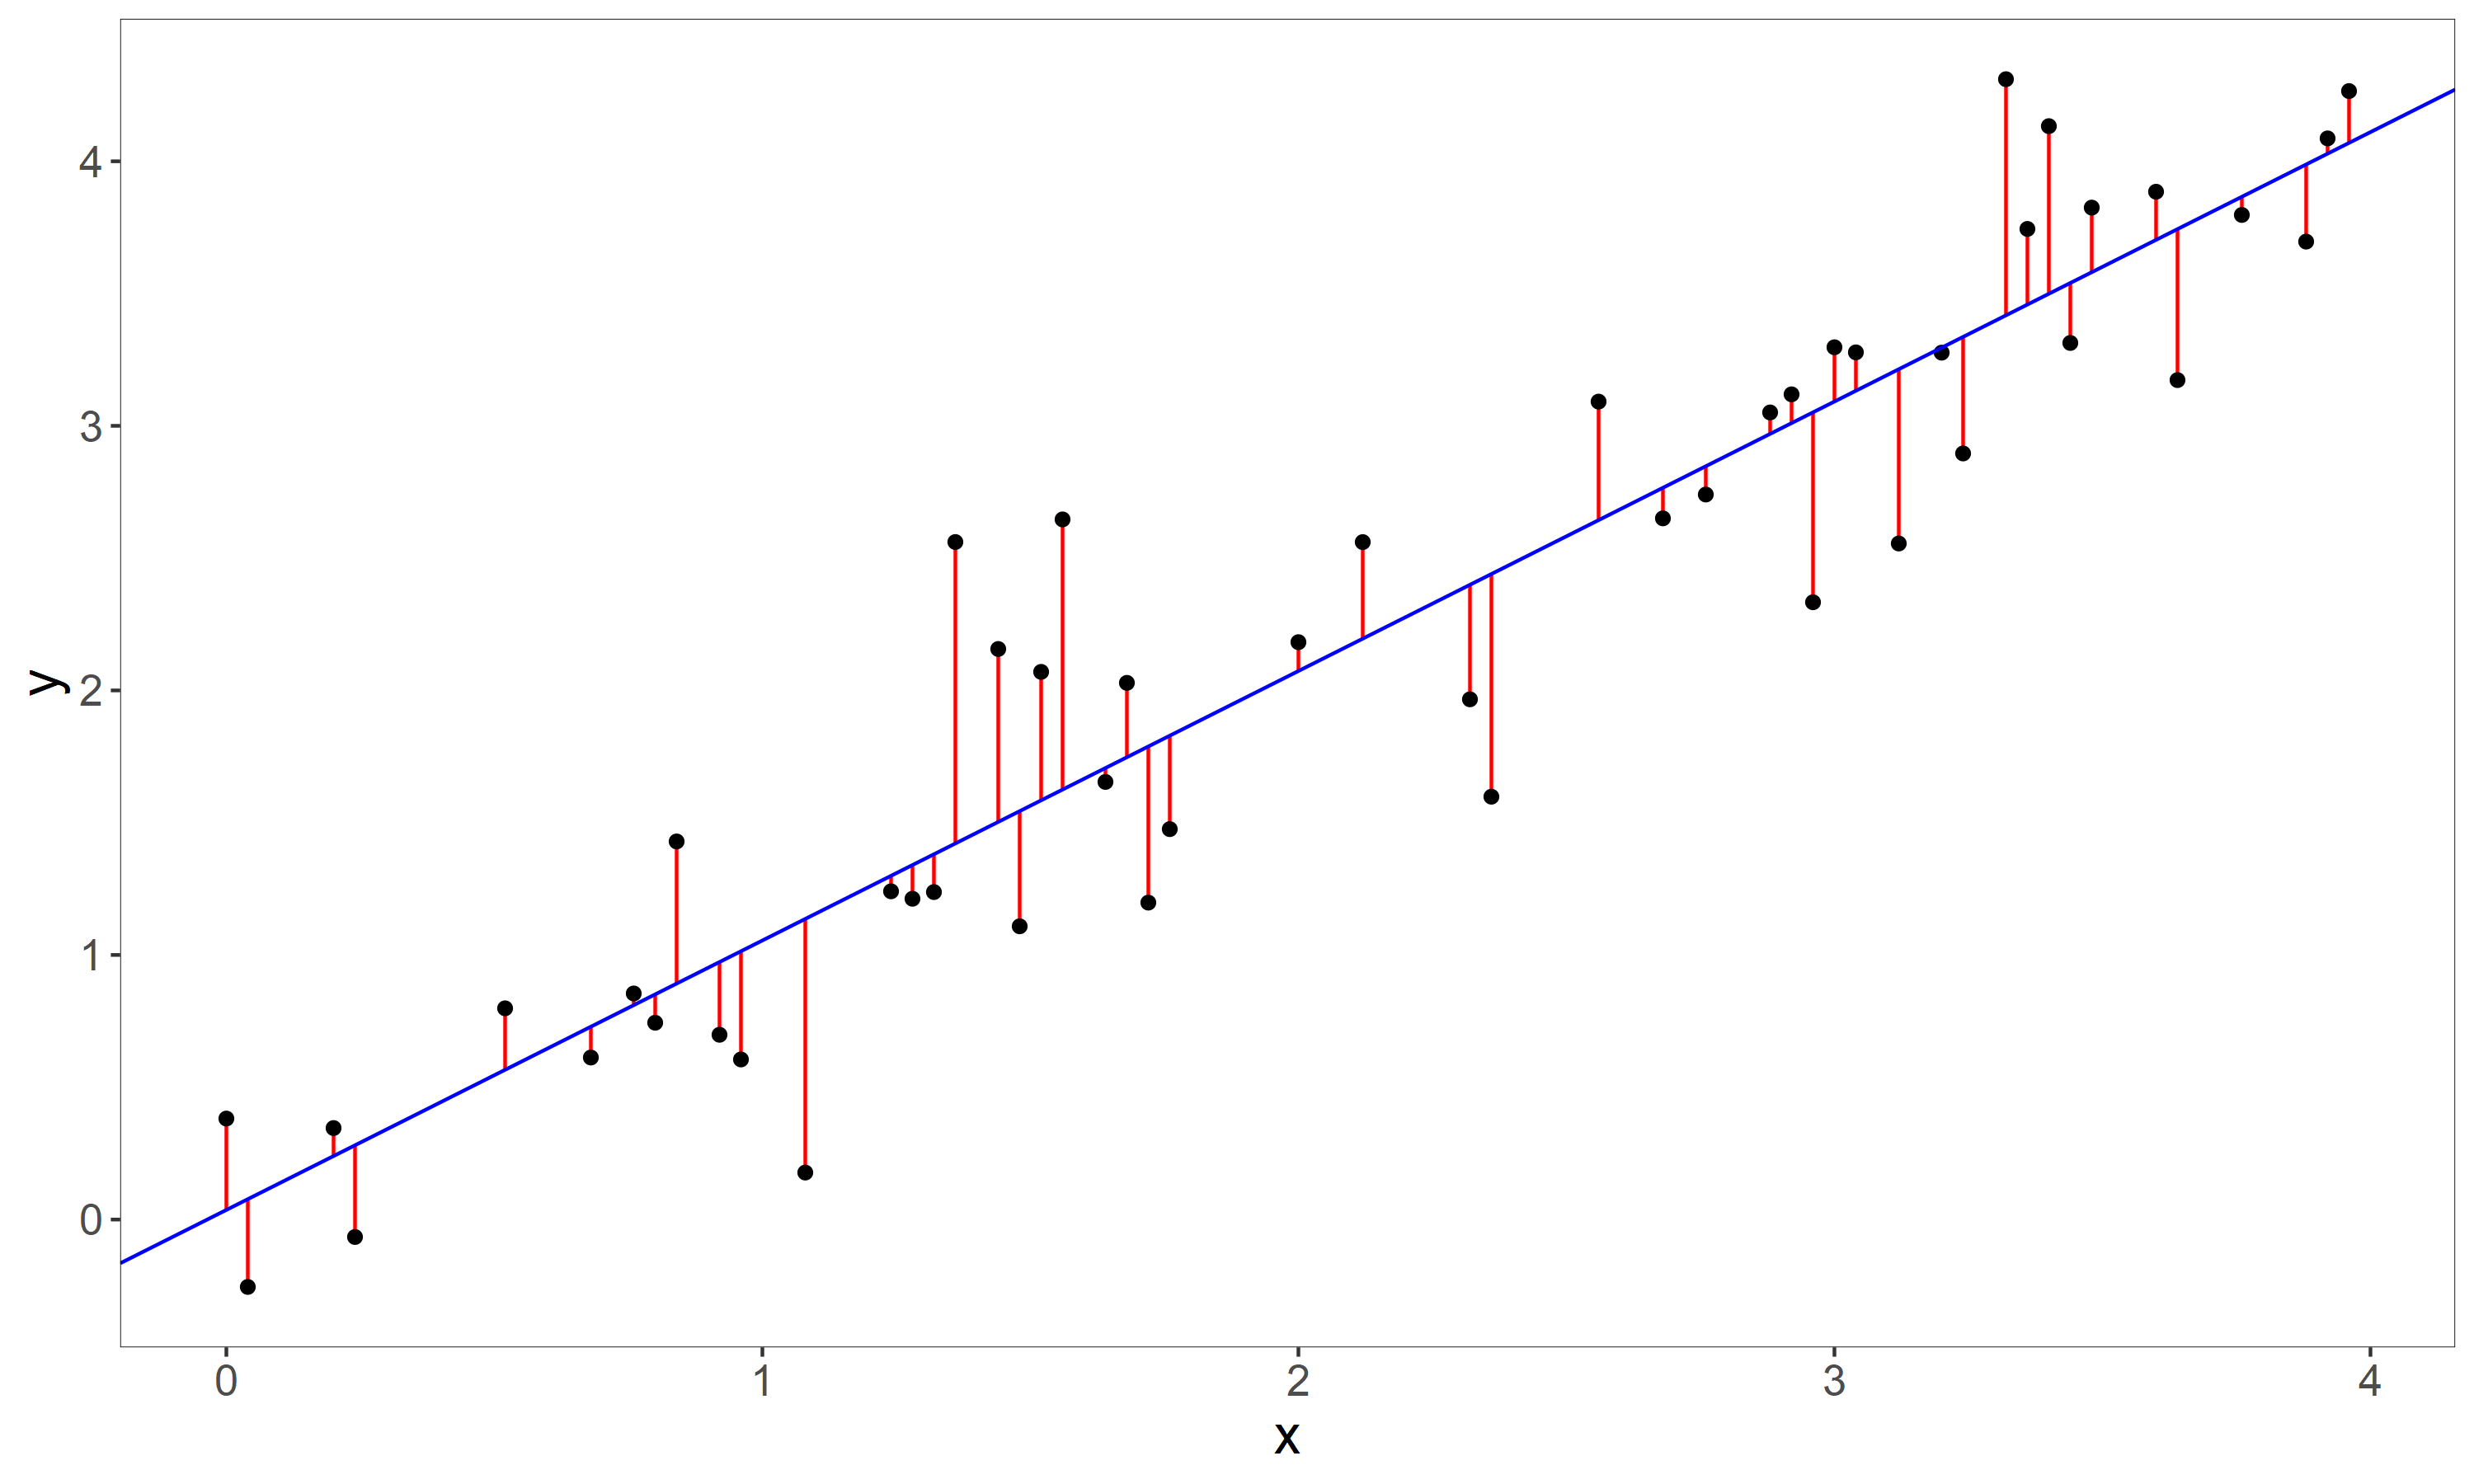
\includegraphics[width = 0.8\textwidth]{images/ols.png}
		\captionsetup{width = 0.8\textwidth}
		\caption{Ordinary least squares fitting with one predictor using simulated data. The blue line represents the line found by ordinary least squares, and the red line segments are the residuals.}
		\label{fig:ols}
	\end{figure}
	\end{comment}
	
	The most common method to estimate the coefficients in a linear model is with \textit{ordinary least squares} (OLS), which selects the values $\beta_0, \beta_1, \dotsc, \beta_p$ that minimize the residual sum of squares
	\begin{equation}\label{eqn:RSS}
		\text{RSS} = \sum\limits_{i = 1}^n \Big[y_i - (\hat{\beta}_0 + \hat{\beta}_1 x_{i1} + \hat{\beta}_2 x_{i2} + \cdots + \hat{\beta}_p x_{ip})\Big]^2
	\end{equation}
	
	\begin{comment}
	One reason that ordinary least squares is popular is because it is very easy to compute. Let $\bm{\beta} = [\beta_0, \beta_1, \beta_2, \dotsc, \beta_p]^\top$ be a $(p + 1) \times 1$ vector of coefficient values and let $\mathbf{X}$ be a $n\times (p + 1)$ matrix where each row contains the predictor values for one observation, with an additional value of 1 in the first entry (this extra value corresponds to the intercept coefficient $\beta_0$). Then $\mathbf{X}\bm{\beta}$ is a vector of the estimated response values for our choice of $\beta$. Let $\mathbf{y}$ represent the true response values. Thus, $\mathbf{y} - \mathbf{X}\bm{\beta}$ is a vector of residuals. To choose coefficient estimates that minimize the residual sum of squares, we compute
	\begin{equation}
		\hat{\bm{\beta}}^{\text{OLS}} = \argmin{\bm{\beta}}{(\mathbf{y} - \mathbf{X}\bm{\beta})^\top (\mathbf{y} - \mathbf{X}\bm{\beta})}
	\end{equation}
	where $(\mathbf{y} - \mathbf{X}\bm{\beta})^\top (\mathbf{y} - \mathbf{X}\bm{\beta})$ is the same residual sum of squares seen in Equation \ref{eqn:RSS}. From \cite{friedman2001elements}, this gives us the solution
	\begin{equation}\label{eqn:ols-solution}
		\hat{\bm{\beta}}^{\text{OLS}} = (\mathbf{X}^\top \mathbf{X})^{-1} \mathbf{X}^\top \mathbf{y}
	\end{equation}
	
	Another advantage of ordinary least squares is that it is an unbiased linear model. This means that if the relationship between the response variable and the predictors is actually linear (as given in Equation \ref{eqn:linear-model}), then the expected value of the coefficient vector $\hat{\bm{\beta}}^\text{OLS}$ is equal to the actual coefficient vector $\bm{\beta}$. Furthermore, the \textit{Gauss-Markov theorem} states that if the random error $\epsilon$ is independent and has constant variance, then ordinary least squares has the lowest variance among all linear unbiased estimators \cite{greene2003econometric, friedman2001elements}. In other words, the coefficient estimates given by ordinary least squares are relatively close to the actual coefficient values when compared to other unbiased linear estimators. This makes ordinary least squares a relatively consistent model.
	\end{comment}
	
	\begin{comment}
	If ordinary least squares is unbiased and has the lowest variance among all unbiased models, why should we use any other type of linear model? Despite having a lower variance than other unbiased models, ordinary least squares can still have a high variance. This is especially an issue when the number of predictors $p$ is large compared to the number of observations $n$. As $p$ gets closer to $n$, a model fitted with ordinary least squares will typically \textit{overfit} to the training set \cite{james2013introduction, friedman2001elements}. This means that the fitted model makes very good predictions with the training data, but performs poorly when given test data that wasn't used to fit the model. Overfitting occurs because of the random error from Equation \ref{eqn:relationship}. Ordinary least squares is unable to distinguish between signal and noise, so it will tend to assume predictors are more strongly related to the response than they actually are.
	
	In the extreme case where $p$ exceeds $n$, the matrix $\mathbf{X}^\top \mathbf{X}$ from Equation \ref{eqn:ols-solution} becomes non-invertible \cite{friedman2001elements}. This means that there are many coefficient estimates that minimize the residual sum of squares. In fact, any of these coefficient estimates creates a perfect fit to the training data, which will result in very bad predictions with test data \cite{james2013introduction}.
	\end{comment}
	
	OLS is common because it is the best linear unbiased estimator; that is, OLS has a lower variance than any other linear unbiased estimator \cite{greene2003econometric, friedman2001elements}. However, if the number of predictors $p$ is large compared to the number of observations $n$, OLS will overfit to the training data. Furthermore, if $p$ exceeds $n$, then the OLS has infinitely many solutions that simply interpolate the training data. In these cases, OLS becomes unreliable for making predictions on test data.
	
	Other types of linear models can overcome this large $p$ small $n$ problem by introducing a small amount of bias. In many cases, these models can perform \textit{variable selection} by setting the coefficients of unimportant predictors to zero. There are several ways to implement variable selection into a linear model. \textit{Filter methods} work by evaluating the ability for each individual predictors to predict the response; then, a model is fit using the predictors selected \cite{sanchez2007filter, ding2005minimum}. \textit{Wrapper methods} fit models using different subsets of predictors and choose the model that has the best performance \cite{guyon2003introduction, liu2020logsum}. Finally, \textit{embedded methods} perform variable selection during the model training process \cite{guyon2003introduction, liu2020logsum}. This paper focuses on wrapper methods and embedded methods. In addition, we considered several non-linear machine learning methods to draw a comparison between linear regression models and machine learning models.
	
	\subsection{Subset Selection Methods}
	% We can review some relevant literature such as Tibshrani et. al. lasso methods, ridge regression, enet, SCAD, or whatever else we want to do.
	
	\textit{Subset selection methods} are wrapper methods that attempt to find a subset of the predictors $X_1, X_2, \dotsc, X_p$ that are most correlated with the response variable $Y$. These algorithms usually fit models for many different subsets and choose the subset of predictors that results in the best model. Although subset selection techniques can be applied to many types of models, we will focus on subset selection with linear regression.
	
	There are two main benefits to using subset selection methods. By reducing the set of available predictors to just those that are strongly related to the response, overfitting can be mitigated. Another benefit of subset selection is that it creates a more interpretable model. If a data set includes thousands of predictors but only a few are related to the response, a model found using subset selection will be easier to understand than a model that relies on all of the parameters. 
	
	\begin{comment}
	\textit{Best subset selection} is a subset selection method that considers every possible combination of predictors. For every possible value of $k$ between 0 and $p$, best subset selection will fit the ${p\choose k}$ possible models using $k$ predictors. Then, the best model for each value of $k$ is chosen based on some performance metric. A final model can be selected from the $(p + 1)$ remaining models, ranging from an empty model with no predictors to a full model with all of the predictors. If $p$ is larger than $n$, then models are only fit for subsets with $n$ or less predictors since ordinary least squares cannot be used when there are more predictors than observations.
	
	Although best subset selection is guaranteed to find the subset of predictors that optimize the chosen metric, this method is computationally expensive. For a data set with $p$ predictors, $2^p$ possible combinations must be considered. This makes best subset selection infeasible when the number of predictors is above 40.
	\end{comment}
	
	\begin{comment}
	Two alternative methods to best subset selection are \textit{forward selection} and \textit{backward selection}. Forward selection begins by fitting a model with no predictors (only the intercept is non-zero) and iteratively adds predictors into the model. The predictor added at each step is chosen to best increase the model fit. Conversely, backward selection starts from the full (ordinary least squares) model with all $p$ predictors and repeatedly removes predictors. Then, like best subset selection, the final model is chosen from the candidate models fitted at each step. Note that backward selection can only be used when $p\leq n$ since ordinary least squares cannot be used when $p>n$. Forward selection can always be used.
	
	Although forward and backward selection will not always encounter the best possible model, these methods help optimize best subset selection and are quicker than best subset selection. Consequently, forward and backward selection can be used for larger values of $p$. However, despite these optimization, forward and backwards selection are still plagued by the fact that the number of combinations of predictors increases exponentially and thus they cannot be used for very large values of $p$.
	
	The models produced by forward and backward selection can be improved by allowing predictors to be added and removed in the same algorithm. \textit{Forward stepwise selection} begins with an empty model and iteratively improves the model by either adding a new predictor or removing an obsolete one. \textit{Backward stepwise selection} works in the same way but starts with the full model. Like backward selection, backward stepwise selection can only be used when $p\geq n$. These techniques take longer to run than ordinary forward and backward selection, but they are more likely to find the best possible model.
	
	When fitting a model using any of the subset selection methods, the performance metric used to select the best model is very important. At first, it may seem reasonable to choose a metric such as the residual sum of squares from Equation \ref{eqn:RSS}. However, many metrics, including the residual sum of squares, only describe a model's performance on training data. This is problematic because including more predictors will always decrease the residual sum of squares on the training data. If $p\leq n$, then the model fitted with all $p$ predictors is exactly the same model produced by ordinary least squares, which by definition minimizes the residual sum of squares! If $p>n$, then a model with the maximum possible number of predictors would be selected.
	
	If we wish to produce a model that makes reliable predictions on test data, we must use a different performance metric. Two of the most common metrics used for this purpose are the \textit{Akaike information criterion} (AIC) and the \textit{Bayesian information criterion} (BIC) \cite{akaike1998information, schwarz1978estimating}. For a given model, the Akaike information criterion can be computed by
	\begin{equation}
		\text{AIC} = 2p - 2\ln(L)
	\end{equation}
	where $p$ is the number of predictors for the model and $L$ is the likelihood of the model. This likelihood represents how well a model fits to the training data. The purpose of the term $2p$ is to punish models with a large number of coefficients. The model with the lowest AIC is the one selected by the wrapper methods.
	
	The Bayesian information criterion very similar to the Akaike information criterion; it is given by
	\begin{equation}
		\text{BIC} = p\ln(n) - 2\ln(L)
	\end{equation}
	where again $p$ is the number of predictors for the model and $L$ is the likelihood of the model.
	
	Note that if $n>7$, then $\ln(n)>2$ and so the penalty for BIC is larger than the penalty for AIC. Hence, a model selected using BIC will typically have fewer parameters than a model selected by AIC.
	
	In addition to AIC and BIC, there are several other metrics that modify training error to estimate test error, such as $C_p$ and adjusted $R^2$ \cite{james2013introduction}. However, this paper will focus on AIC and BIC.
	\end{comment}
	
	\textit{Best subset selection} is a wrapper method that fits and evaluates models using every possible subset of predictors. Although this method is guarenteed to find the optimal model for some evaluation metric, it is computationally infeasible with a large number of predictors \cite{miller2002subset}. In many cases, using more greedy algorithms can lead to comparable results.
	
	\textit{Forward stepwise selection} starts by fitting a model with none of the predictors (by simply estimating each observation to be the mean of the response). The algorithm then iteratively chooses the predictor that best increases the model fit until a stopping condition is met. \textit{Backward stepwise selection} does the same thing, but starts with a full model and works backwards. In addition, \textit{forward stepwise selection} and \textit{backward stepwise selection} are hybrid techniques that can both add and remove predictors in each iteration. Note that backward selection and backward stepwise selection can only be used when $p < n$, since they rely on starting on a full OLS model.
	
	Despite improving the computational costs associated with best subset selection, these alternative algorithms must still fit a massive number of models for large values of $p$. Consequently, the embedded methods discussed next are often favored. 
	
	\subsection{Penalized Regression}
	
	In general, \textit{penalized regression} works by fitting a model that punishes large coefficient estimates. By forcing coefficient values to shrink, the resulting model will have relatively low variance. Most, but not all, of these methods can perform variable selection during the fitting process, making them a type of embedded method.
	
	Almost all of the penalized regression methods in this paper solve an optimization problem of the form
	\begin{equation}\label{eqn:penalized-regression-lambda}
		\hat{\bm{\beta}}=\argmin{\bm{\beta}}{\sum\limits_{i = 1}^n \Big[y_i - (\beta_0 + \beta_1 x_{i1} + \beta_2 x_{i2} + \cdots + \beta_p x_{ip})\Big]^2 + \sum\limits_{j = 1}^p P(\beta_j)}
	\end{equation}
	where the first summation is the usual residual sum of squares and $P(\beta)$ is a penalty function that is applied to every coefficient (besides $\beta_0$). Usually, this penalty depends on at least one tuning parameter (usually denoted by $\lambda$) that controls how strong the penalty is. A suitable choice for the tuning parameter(s) will lead to a well-performing model.
	\begin{comment}
	In general, $P(\beta)$ is an even function that is non-decreasing as $\vert \beta \vert$ increases. If $\lambda = 0$, then we have the usual ordinary least squares estimator. As $\lambda$ increases, a stronger penalty is applied which will decrease the coefficient values. As $\lambda$ approaches $\infty$, the model becomes an empty model where only the intercept term is non-zero.
	\end{comment}
	
	\begin{comment}
	A similar way to express penalized regression is with the form
	\begin{equation}\label{eqn:penalized-regression-t}
		\hat{\bm{\beta}} = \argmin{\bm{\beta}}{\sum\limits_{i = 1}^n \Big[y_i - (\beta_0 + \beta_1 x_{i1} + \beta_2 x_{i2} + \cdots + \beta_p x_{ip})\Big]^2} \quad \text{subject to} \quad \sum\limits_{j = 1}^p P(\beta_j)\leq t
	\end{equation}
	where $t$ is a hyperparameter \cite{james2013introduction, friedman2001elements}. In this form, penalized regression fits the ordinary least squares under the condition that the sum of the penalties of the coefficients is kept below some threshold. It can be shown that for every value of $\lambda$ from Equation \ref{eqn:penalized-regression-lambda}, there is a value of $t$ from Equation \ref{eqn:penalized-regression-t} that gives equivalent coefficient estimates \cite{james2013introduction}. Most algorithms to fit penalized regression models use the form given in Equation \ref{eqn:penalized-regression-lambda}, but the form in Equation \ref{eqn:penalized-regression-t} may be considered more intuitive.
	
	When fitting penalized regression models, the choice of $\lambda$ is very important. If $\lambda$ is too small, then models may be overfit just like ordinary least squares; on the other hand, if $\lambda$ is large, then the resulting models are highly biased and the resulting models may be underfit. In practice, the best value of $\lambda$ can be selected using \textit{cross validation} and \textit{grid search}. This process involves splitting the training set into $k$ disjoint subsets of equal size called \textit{folds}. Then, $k$ models are fitted for different values of $\lambda$, where one fold is used as a testing set and the other $(k - 1)$ folds are used for training. The value of $\lambda$ that results in the lowest test error can then be selected.
	\end{comment}
	
	\textit{Ridge regression} is a penalized linear regression model that uses the penalty function $P(\beta) = \lambda\beta^2$, where $\lambda$ is a tuning parameter \cite{hoerl1970ridge}.
	\begin{comment}
	One advantage of ridge regression is that it can handle highly correlated data better than ordinary least squares. When predictors are correlated with each other, some algorithms have a hard time distinguishing which predictors are actually related to the response.
	\end{comment}
	Ridge regression benefits from having a relatively simple solution and its ability to handle colinearity; however, it is unable to perform variable selection.
	
	\begin{comment}
	One drawback of ridge regression is that it cannot perform variable selection. It can shrink coefficients towards zero, but it cannot set coefficients to be exactly zero.
	\end{comment}
	
	The \textit{least absolute shrinkage and selection operation} (lasso) is a shrinkage method with a very similar form to ridge regression \cite{tibshirani1996regression, james2013introduction}. The penalty function for lasso is $P(\beta) = \lambda\vert \beta \vert$. Unlike ridge regression, the lasso can perform variable selection.
	
	\begin{comment}
	Unlike ridge regression, lasso regression can perform variable selection by setting coefficients to zero. This makes lasso regression favorable when most predictors are not related to the response variable. On the other hand, if the response truly does depend on all of the predictors, then lasso regression may incorrectly set some coefficients to zero. In addition, lasso regression does not have a closed-form solution, but computing the coefficients is still efficient.
	\end{comment}
	
	\begin{comment}
	Figure \ref{fig:ridge-lasso-diagram} provides a visual explanation for why ridge regression cannot perform variable selection while lasso regression can. Suppose that there are $p = 2$ predictors. The red circle in Figure \ref{fig:ridge-diagram} represents the circle $\beta_1^2 + \beta_2^2 \leq t$, which is the penalty boundary for ridge regression using the form given in Equation \ref{eqn:penalized-regression-t} when $t = 1$. The red square in Figure \ref{fig:lasso-diagram} represents the boundary $\vert \beta_1 \vert + \vert \beta_2 \vert \leq t$ for lasso regression. The point in the center of the blue ellipses represents the values of $\beta_1$ and $\beta_2$ that ordinary least squares would estimate. Because this point is not within either of the red regions, ridge regression and lasso regression will give different coefficient estimates. The blue ellipses around this point represent contour curves for the residual sum of squares, which is a quadratic function of $\beta_1$ and $\beta_2$. The first intersection of these ellipses with the red regions represents the coefficient values selected by ridge and lasso regression, since it represents the point within the red region with the lowest residual sum of squares. Because the ridge regression boundary is round, the intersection in Figure \ref{fig:ridge-diagram} occurs when $\beta_1$ and $\beta_2$ are both positive. For lasso regression in Figure \ref{fig:lasso-diagram}, the intersection occurs at a corner where $\beta_1=0$. Thus, lasso regression has set $\beta_1$ to zero, while $\beta_1$ is non-zero for ridge regression.
	
	\begin{figure}[!b]
		\centering
		\begin{subfigure}[b]{0.45\textwidth}
			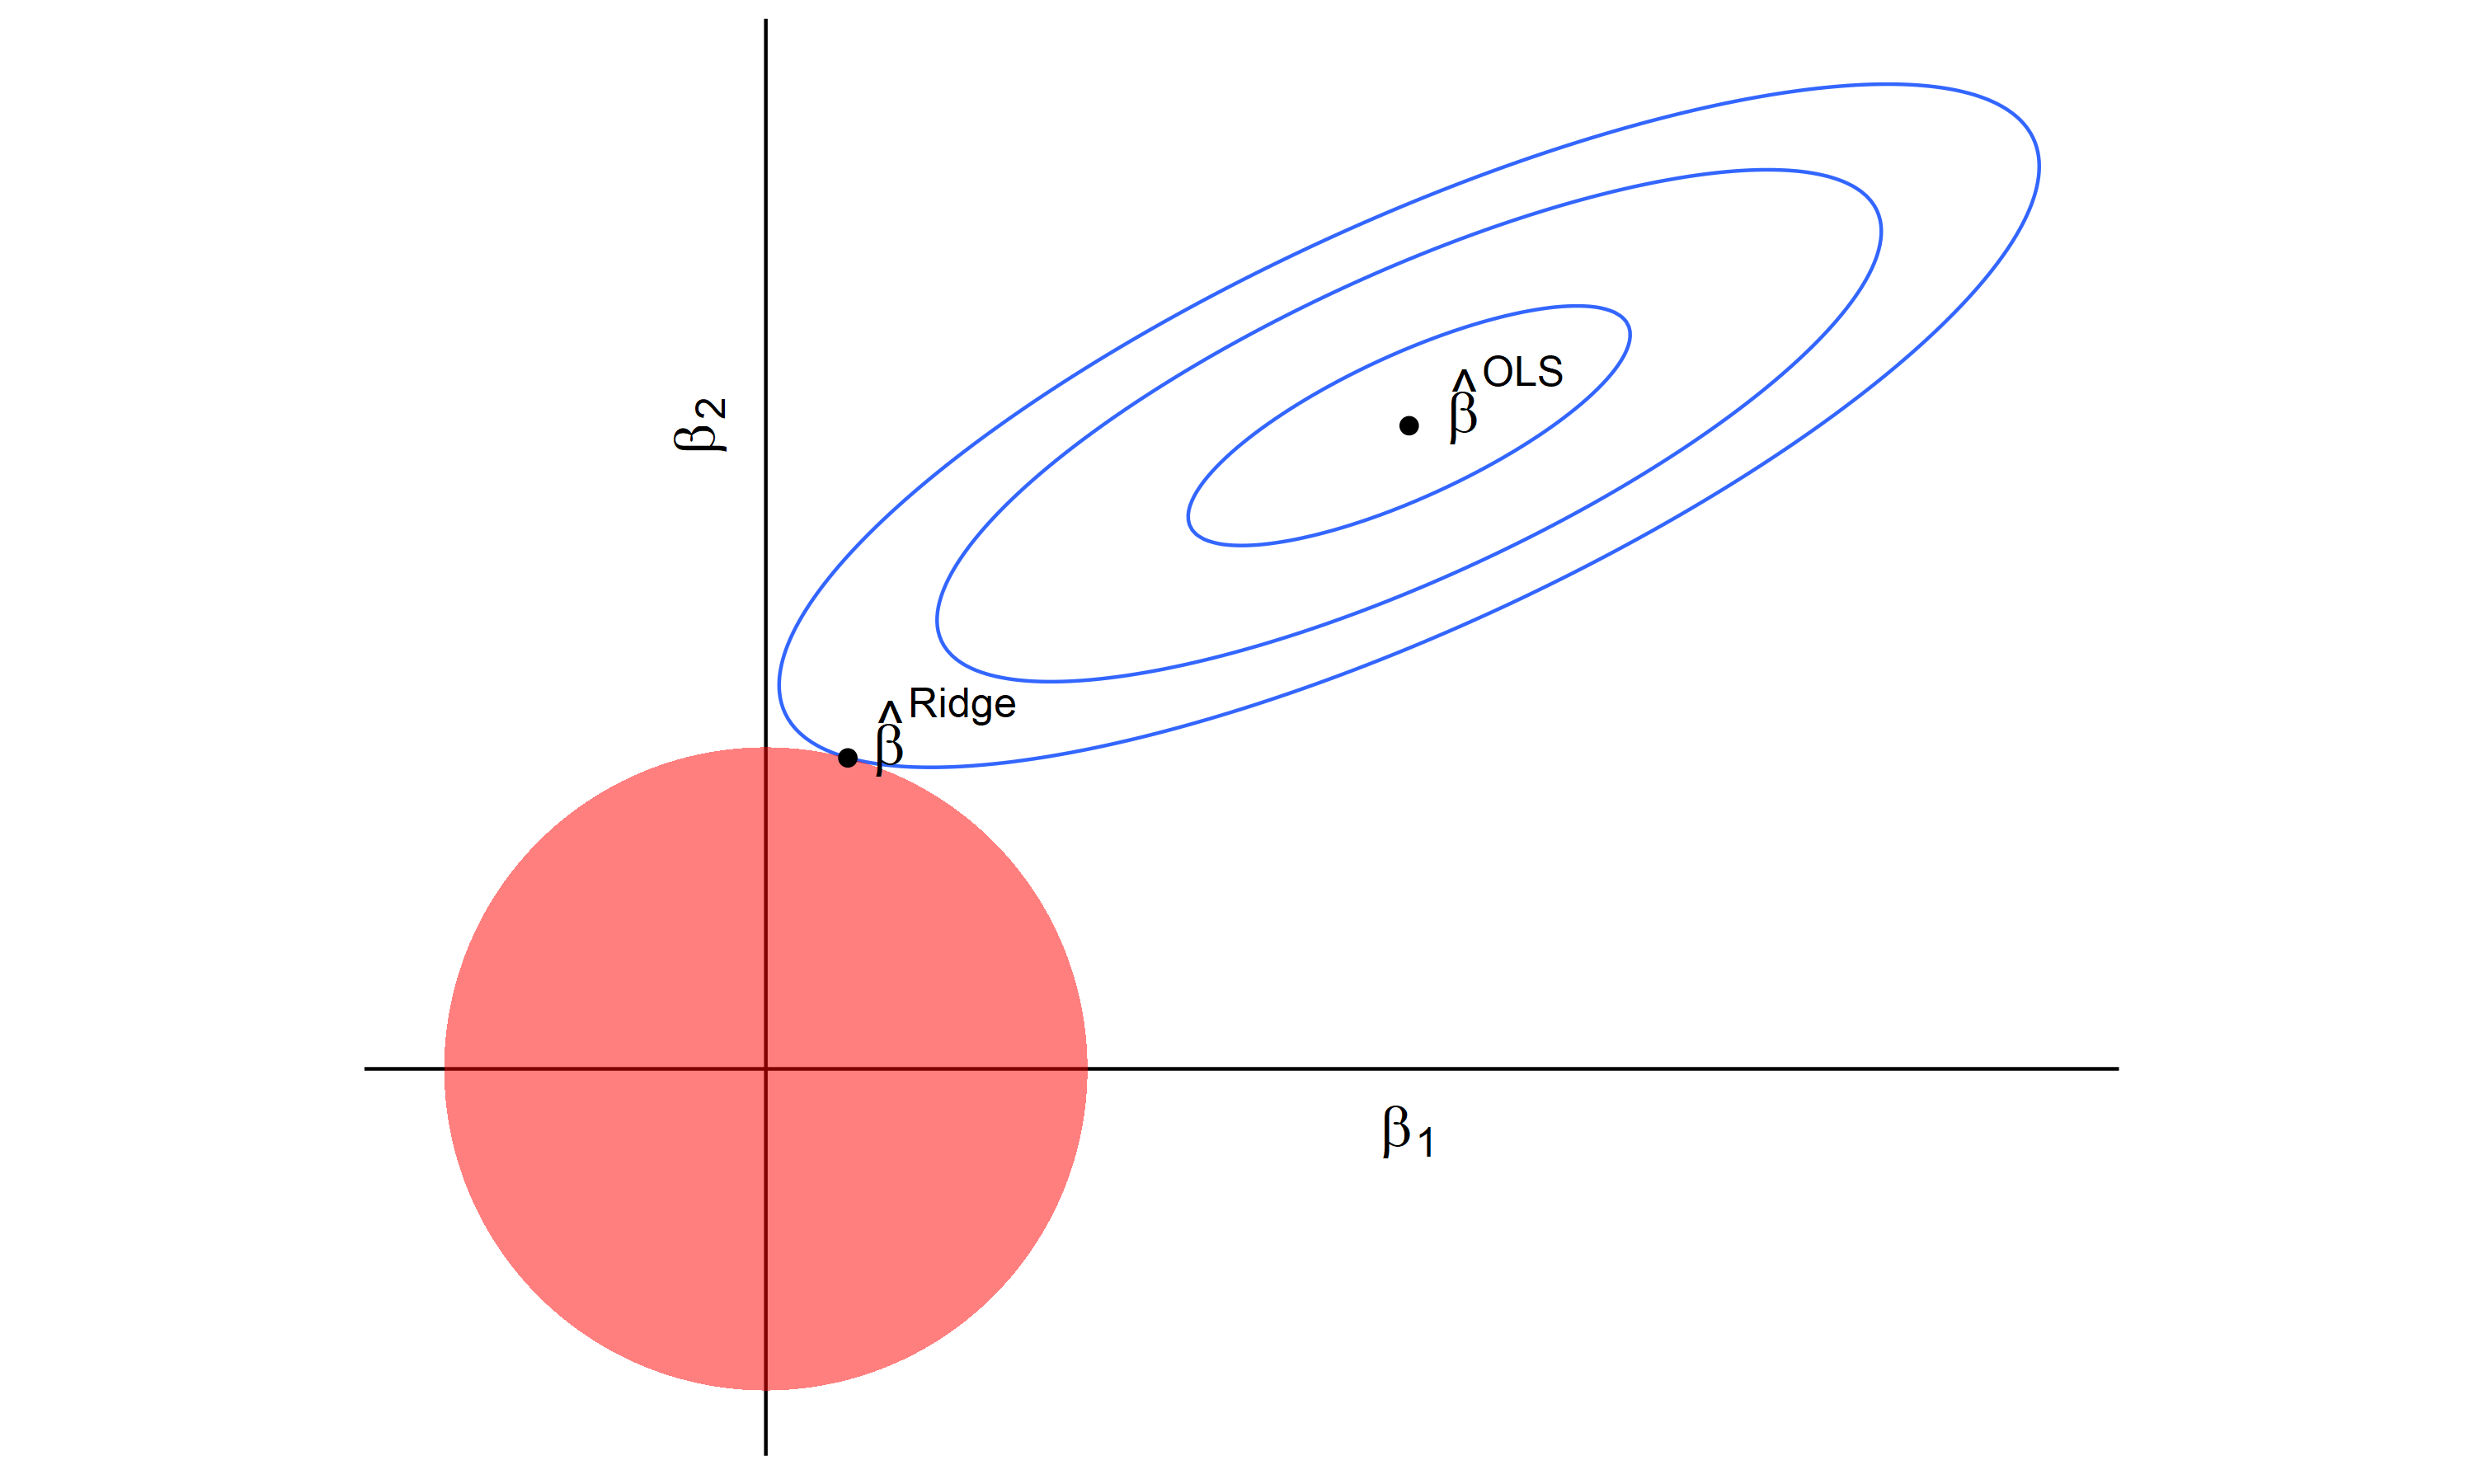
\includegraphics[width=\textwidth]{images/ridge-diagram.png}
			\captionsetup{width = 0.8\textwidth}
			\caption{RSS contours and the ridge penalty boundary.}
			\label{fig:ridge-diagram}
		\end{subfigure}
		\hspace{30pt}
		\begin{subfigure}[b]{0.45\textwidth}
			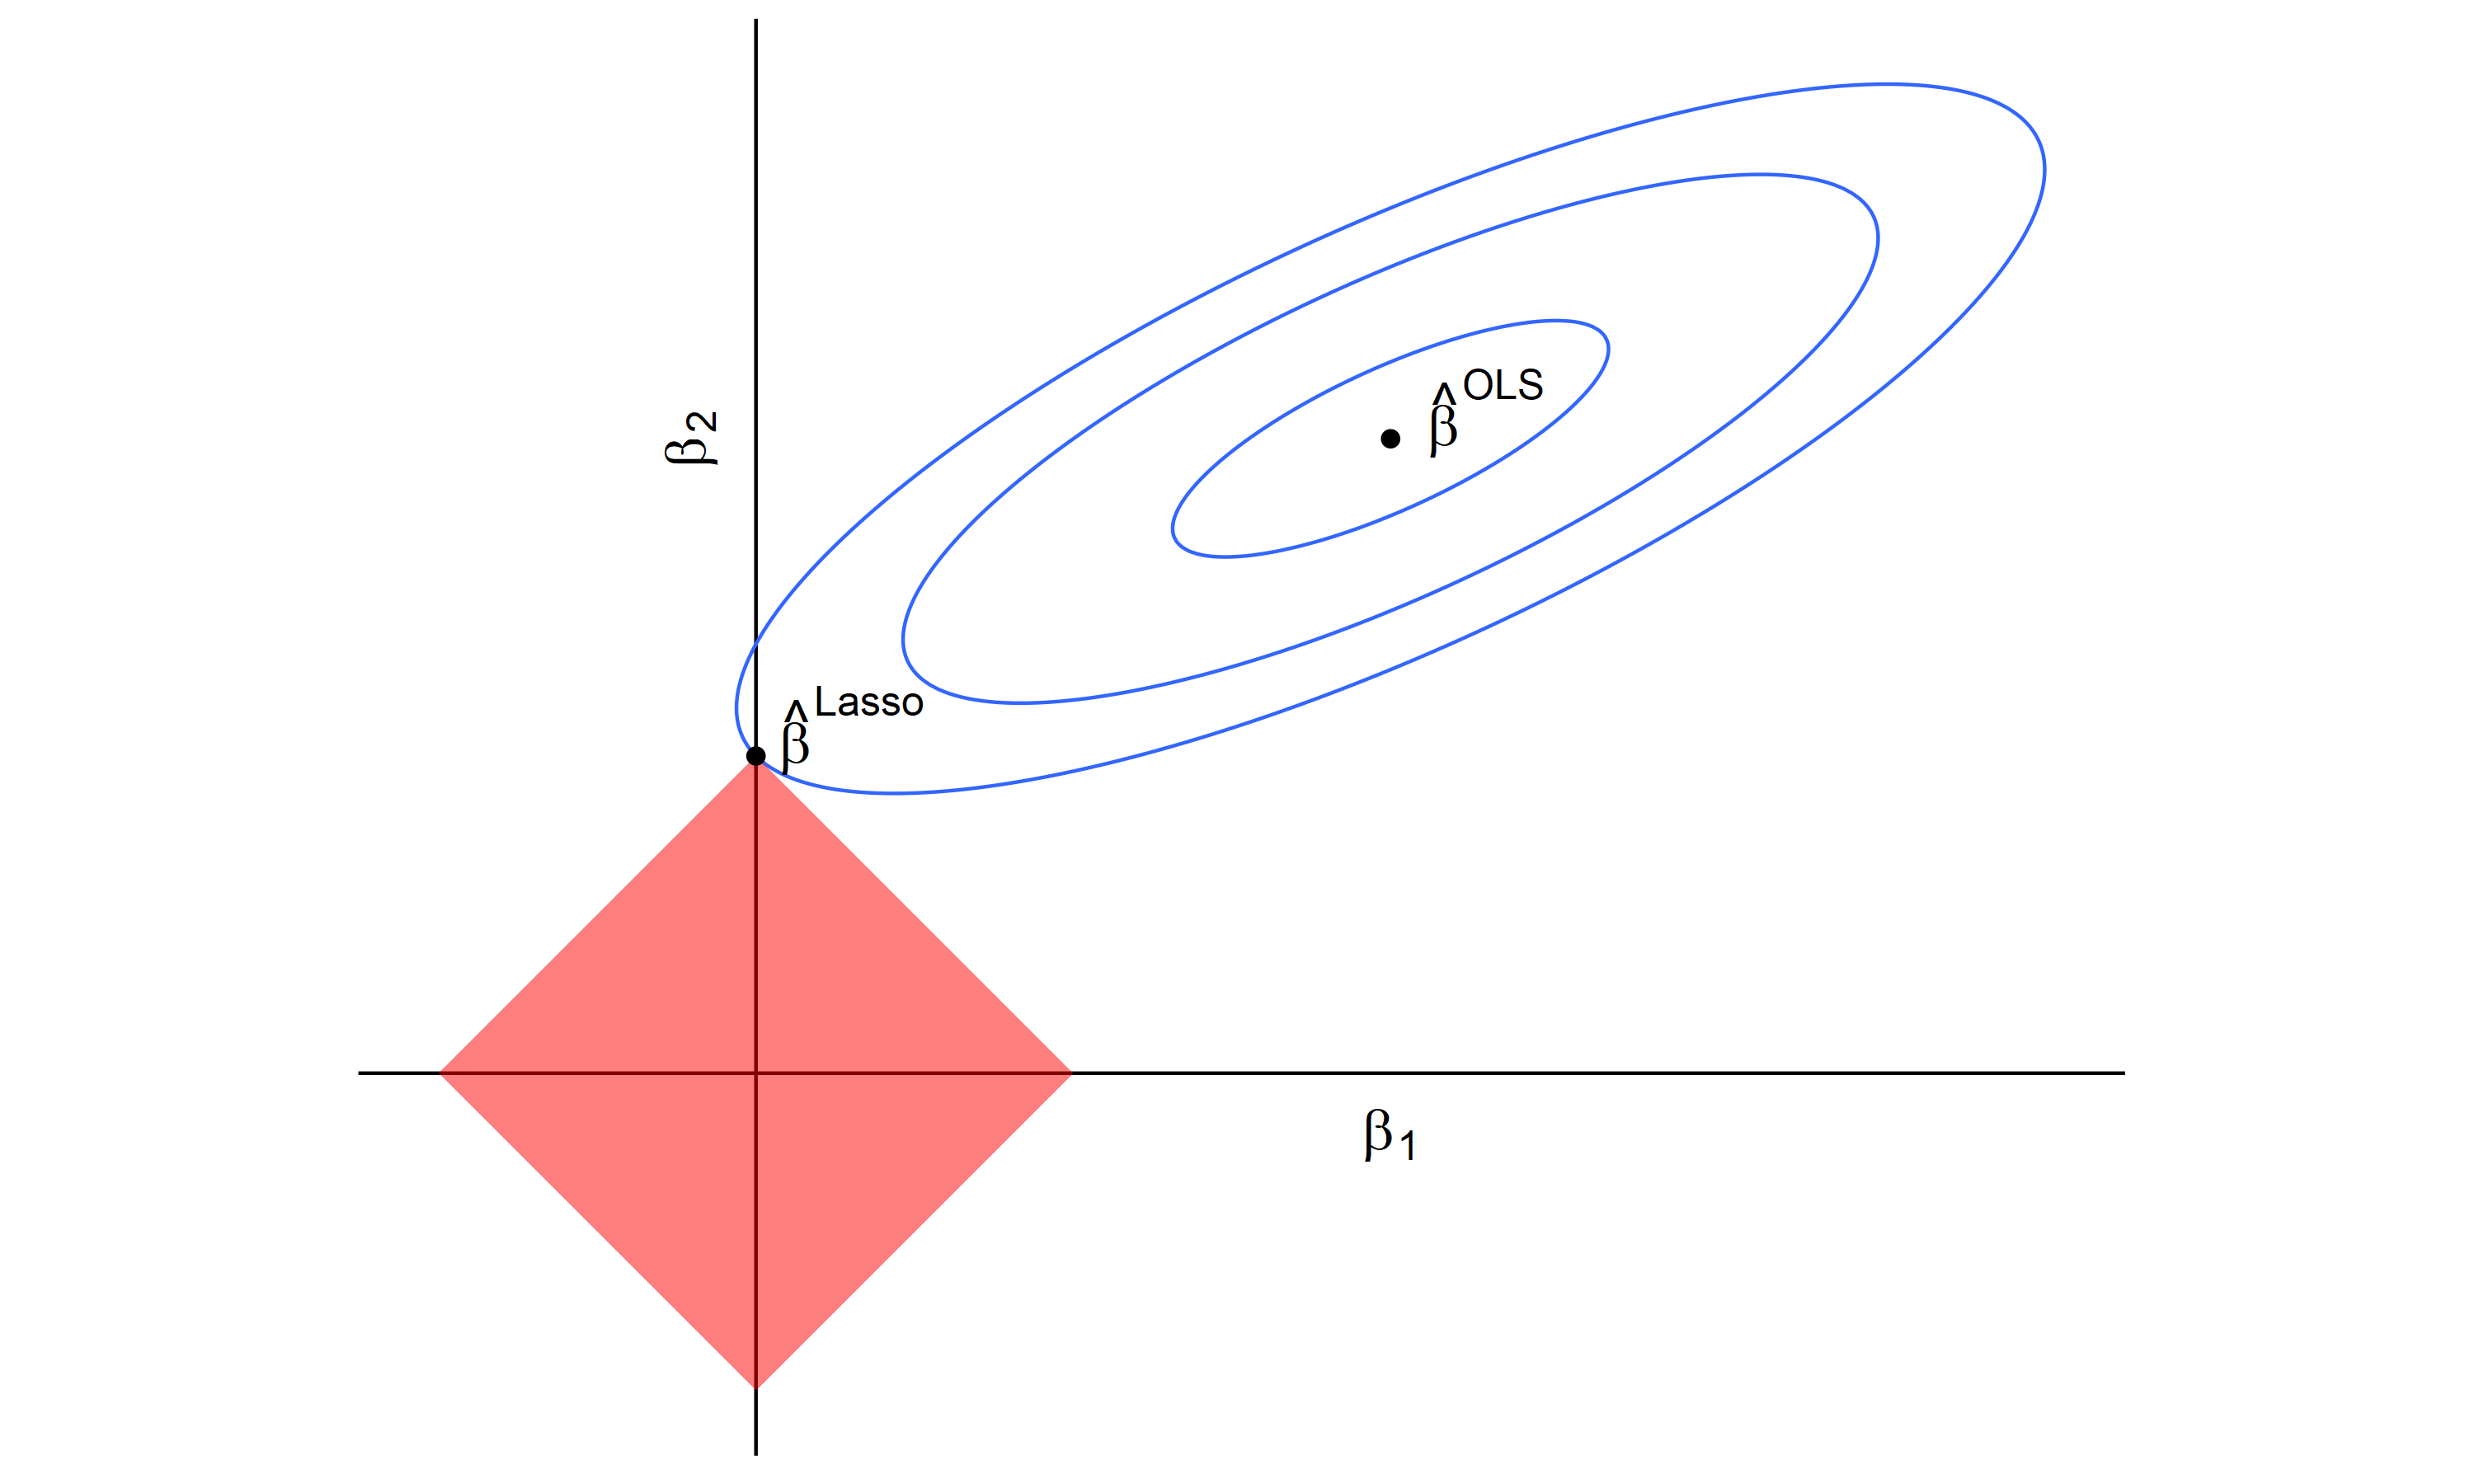
\includegraphics[width=\textwidth]{images/lasso-diagram.png}
			\captionsetup{width = 0.8\textwidth}
			\caption{RSS contours and the lasso penalty boundary.}
			\label{fig:lasso-diagram}
		\end{subfigure}
		\captionsetup{width = 0.9\textwidth}
		\caption{RSS contours and penalty bounds for the ridge and lasso models when $p=2$ and $t = 1$. The red regions represent the coefficient values allowed by ridge and lasso regression, respectively. The blue ellipses represent contours of the residual sum of squares, with $\hat{\beta}^{\text{OLS}}$ being the point where the residual sum of squares is minimized. The intersection of the ellipse with the red region in each plot represents the coefficient values selected by lasso and ridge.}
		\label{fig:ridge-lasso-diagram}
	\end{figure}
	\end{comment}
	
	\begin{comment}
	\textit{Elastic-net} regression uses both the ridge penalty and the lasso penalty at the same time \cite{zou2005regularization}. Elastic-net solves the optimization problem
	\begin{equation}
		\hat{\beta}^{\text{E-net}}=\argmin{\beta}{\sum\limits_{i = 1}^n \Big[y_i - (\beta_0 + \beta_1 x_{i1} + \beta_2 x_{i2} + \cdots + \beta_p x_{ip})\Big]^2 + \lambda_2\sum\limits_{j = 1}^p \beta_j^2 + \lambda_1\sum\limits_{j = 1}^p \vert \beta_j \vert}
	\end{equation}
	where $\lambda_1$ and $\lambda_2$ are both tuning parameters.
	
	An important limitation to note is that elastic net performs best when it close to either ridge or lasso regression, meaning that either $\lambda_1$ greatly exceeds $\lambda_2$ or $\lambda_2$ greatly exceeds $\lambda_1$ \cite{zou2005regularization}. Additionally, because elastic net requires two tuning parameters, this makes it much more difficult to determine the best combination of tuning parameters to minimize error in the regression. However, this problem has been largely solved through by the LARS-EN algorithm developed by Zou et. al. which efficiently solves for the tuning parameters \cite{zou2005regularization}.
	\end{comment}
	
	\textit{Elastic-net} (E-net) regression uses both the ridge penalty and the lasso penalty at the same time by using the penalty function $P(\beta)=\lambda_1 \vert \beta \vert + \lambda_2 \beta^2$, where $\lambda_1$ and $\lambda_2$ are separate tuning parameters \cite{zou2005regularization}.
	
	\begin{comment}
	One major flaw of the lasso method is that the penalty punishes large coefficients, even if those coefficients should be large. One way to modify the lasso method is to use the \textit{smoothly clipped absolute deviation} (SCAD) penalty \cite{fan2001variable}. The goal of this method is to punish large coefficients less severely, which can help mitigate some of the bias introduced by the lasso method. The penalty function $P(\beta)$ for SCAD satisfies
	\begin{equation}\label{eqn:scad-derivative-indicator}
		\frac{dP}{d\beta} = \sign(\beta)\left[ I(\vert \beta \vert<\lambda) + \frac{\max(a\lambda - \vert \beta\vert, 0)}{(a - 1)\lambda}I(\vert \beta \vert > \lambda) \right]
	\end{equation}
	where $a>2$ is a new hyperparameter and $I$ is the indicator function ($I(Q)$ equals 1 if a statement $Q$ is true, and equals 0 if $Q$ is false). If the hyperparameter $a$ is large, then SCAD behaves like lasso for larger coefficient values. Also, notice that $\lambda$ is an argument for the penalty function $P$.
	
	An equivalent way to write the expression in Equation \ref{eqn:scad-derivative-indicator} is
	\begin{equation}
		\frac{dP}{d\beta} = \left\{\begin{array}{ll}
			1,&\vert \beta \vert\leq \lambda\\
			\frac{a\lambda - \vert \beta \vert}{(a - 1)\lambda},&\lambda < \vert \beta \vert < a\lambda\\
			0,&\alpha\lambda < \vert \beta \vert
		\end{array}\right.
	\end{equation}
	This penalty function does not punish coefficients with large magnitude as heavily as the lasso method. In fact, if the magnitude of a coefficient is larger than $a\lambda$, then the penalty becomes constant since the derivative becomes zero.
	
	By integrating with respect to $\beta$ and choosing $P(\beta) = 0$ \cite{breheny2016lasso}, we see that
	\begin{equation}
		P(\beta) = \left\{\begin{array}{ll}
			\vert \beta \vert,&\vert \beta \vert \leq \lambda\\
			\frac{2a\lambda\vert\beta\vert - \beta^2-\lambda^2}{2(a - 1)\lambda},&\lambda < \vert \beta \vert \leq a\lambda\\
			\frac{\lambda(a + 1)}{2},&a\lambda < \vert \beta \vert
		\end{array}\right.
	\end{equation}
	
	The \textit{minimax concave penalty} (MCP) method is very similar to SCAD \cite{zhang2010nearly}. Both methods are used to avoid the high bias caused by the lasso method. MCP uses a penalty function that satisfies
	\begin{equation}
		\frac{dP}{d\beta} = \left\{\begin{array}{ll}
			\sign(\beta)\left(1 - \frac{\vert \beta \vert}{a\lambda}\right),& \vert \beta \vert \leq a\lambda\\
			0,&a\lambda < \vert \beta \vert
		\end{array}\right.
	\end{equation}
	where, like SCAD, $a>0$ is a hyperparameter. Integrating \cite{breheny2016lasso}, we see that
	\begin{equation}
		P(\beta) = \left\{\begin{array}{ll}
			\vert \beta \vert - \frac{\beta^2}{2a\lambda},&\vert \beta \vert \leq a\lambda\\
			\frac{1}{2}a\lambda,&a\lambda < \vert \beta \vert
		\end{array}\right.
	\end{equation}
	\end{comment}
	
	Two additional penalized regression techniques are \textit{Smoothly-Clipped Absolute Deviation} (SCAD) and \textit{Minimax Concave Penalty} (MCP) \cite{fan2001variable, zhang2010nearly}. These methods use more complicated penalty functions that punish larger coefficients less severely. This helps to reduce the bias of the resulting models.
	\begin{comment}
	Figure \ref{fig:lasso-scad-mcp} below shows the penalty functions (and their derivatives) for lasso, SCAD, and MCP as a function of a coefficient value $\beta$. We see that lasso applies a much stronger penalty to large coefficients than SCAD or MCP. Also, note that SCAD starts with a derivative equal to that of the lasso for small values of $\beta$; on the other hand, the derivative of the penalty function for MCP starts decreasing immediately.
	
	\begin{figure}[!h]
		\centering
		\begin{subfigure}[b]{0.45\textwidth}
			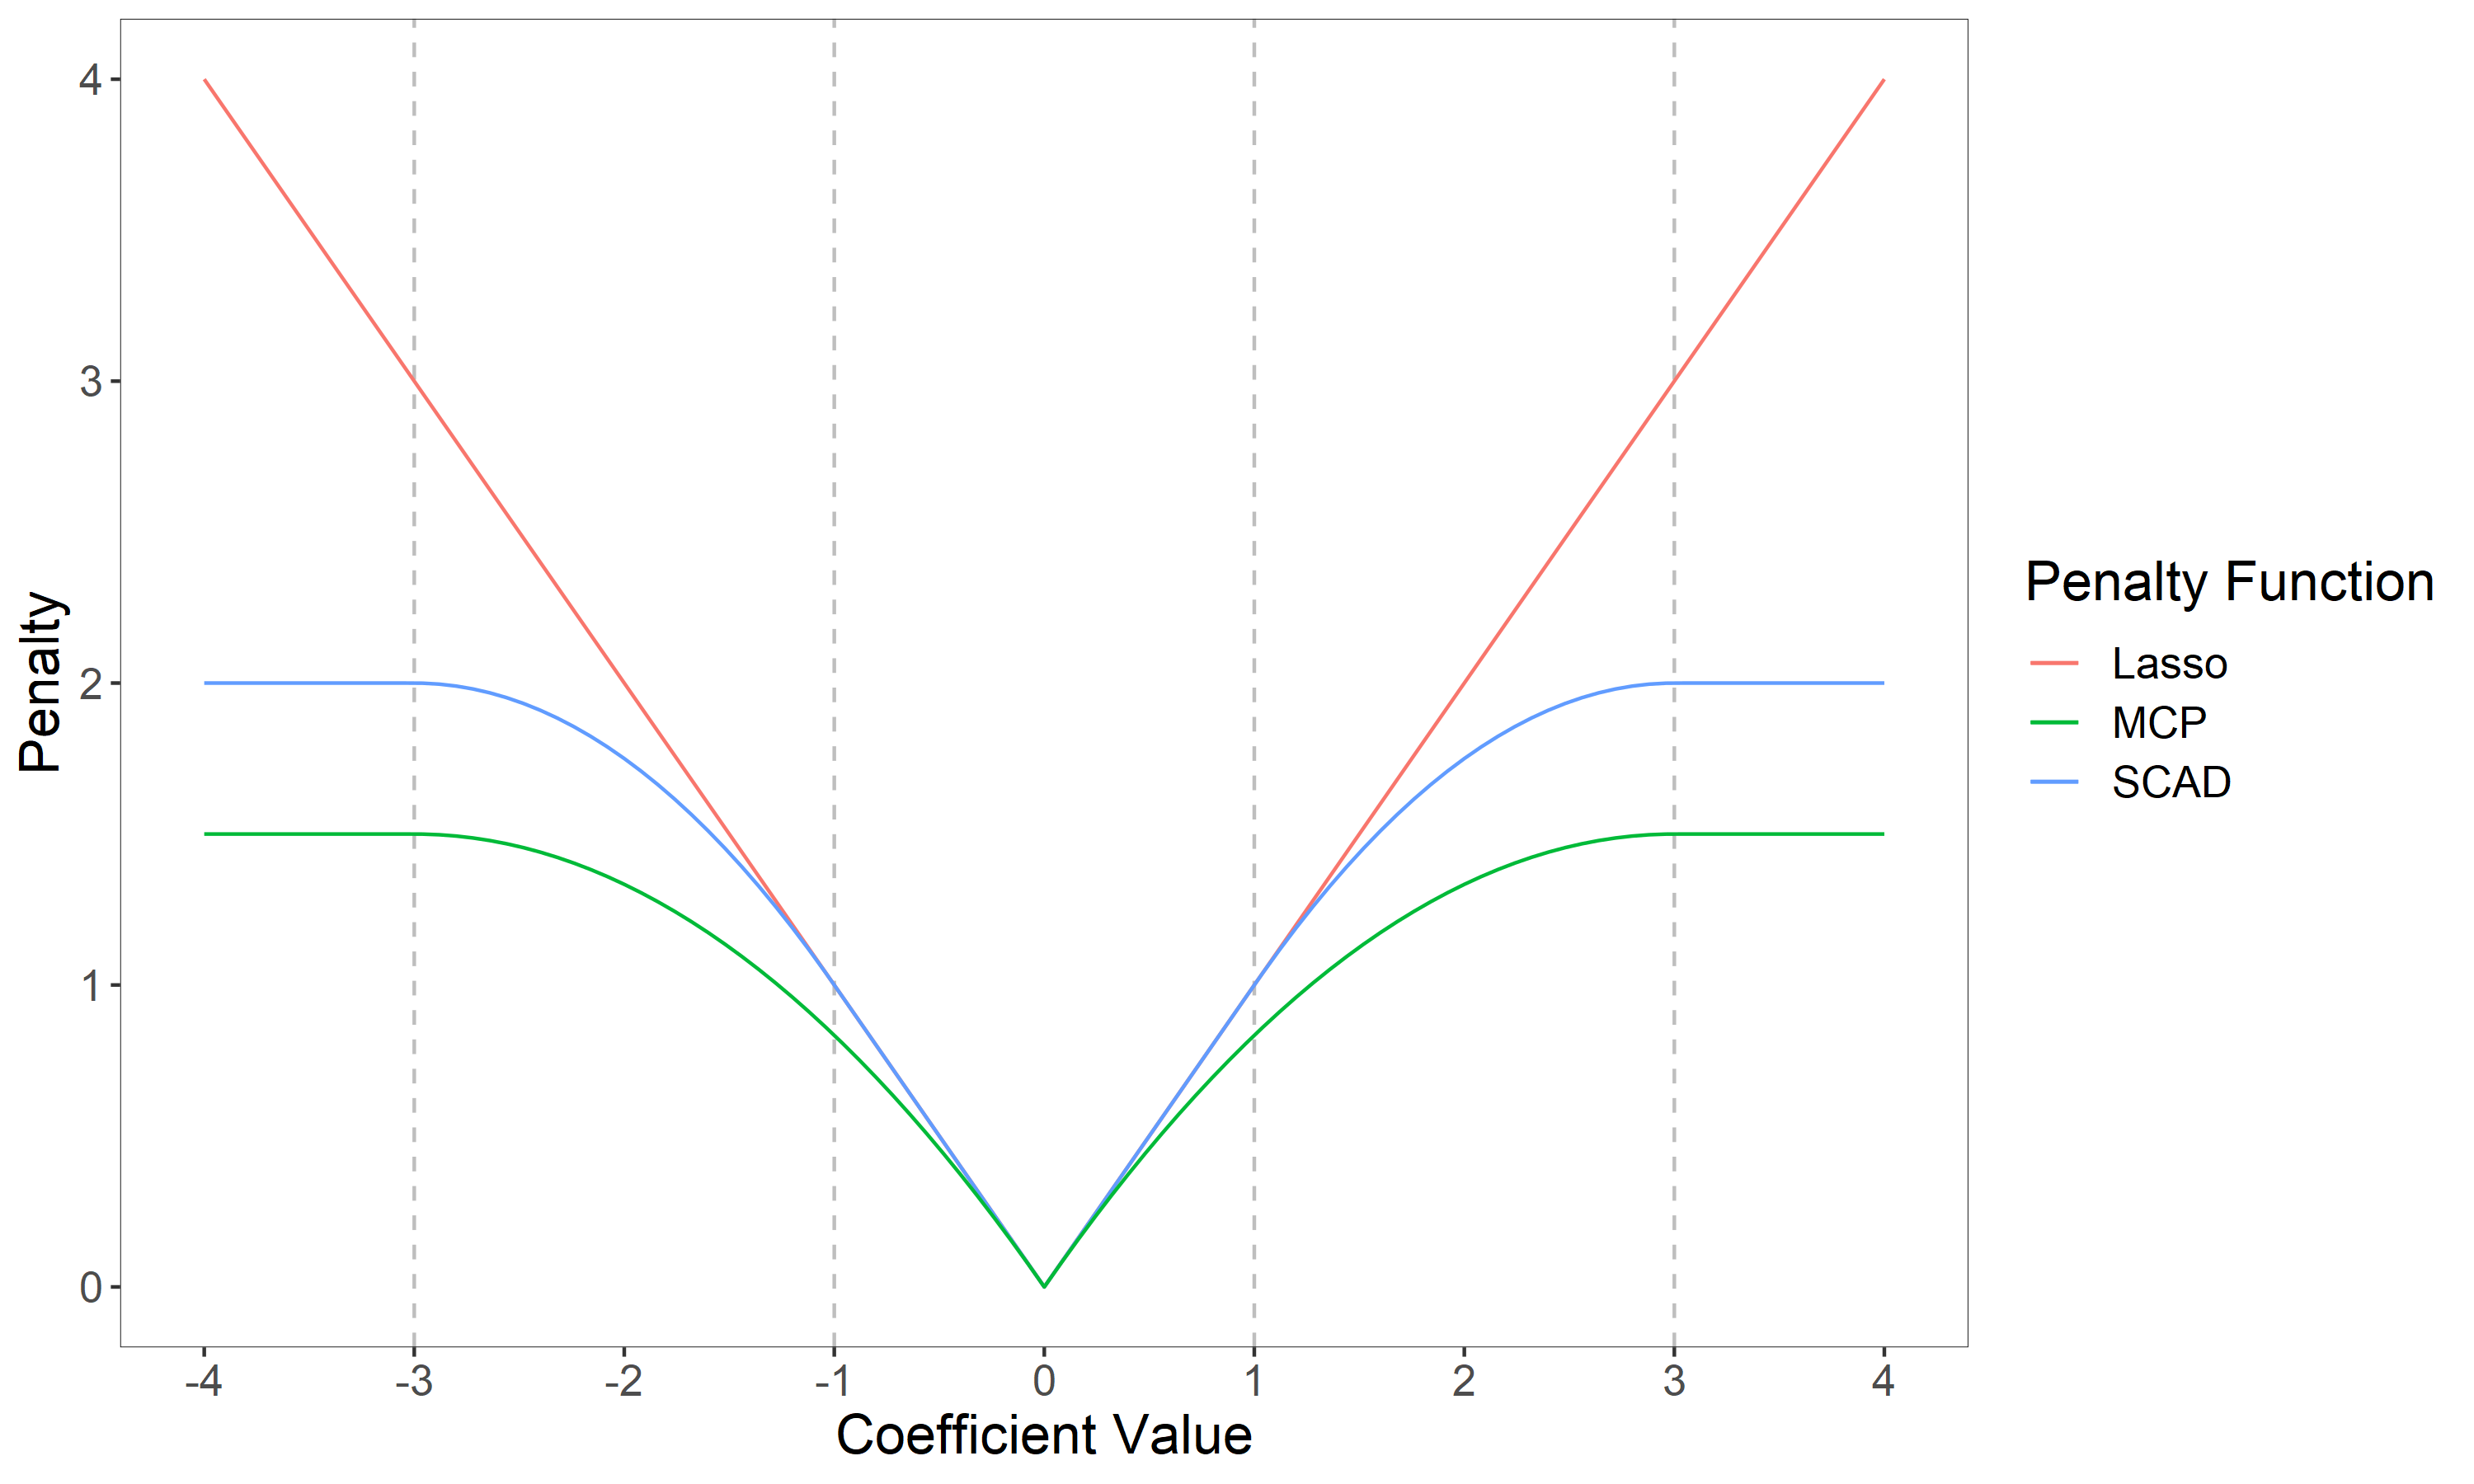
\includegraphics[width=\textwidth]{images/lasso-scad-mcp-penalty.png}
			\captionsetup{width = 0.8\textwidth}
			\caption{Penalty functions for lasso, SCAD, and MCP.}
			\label{fig:penalty}
		\end{subfigure}
		\hspace{30pt}
		\begin{subfigure}[b]{0.45\textwidth}
			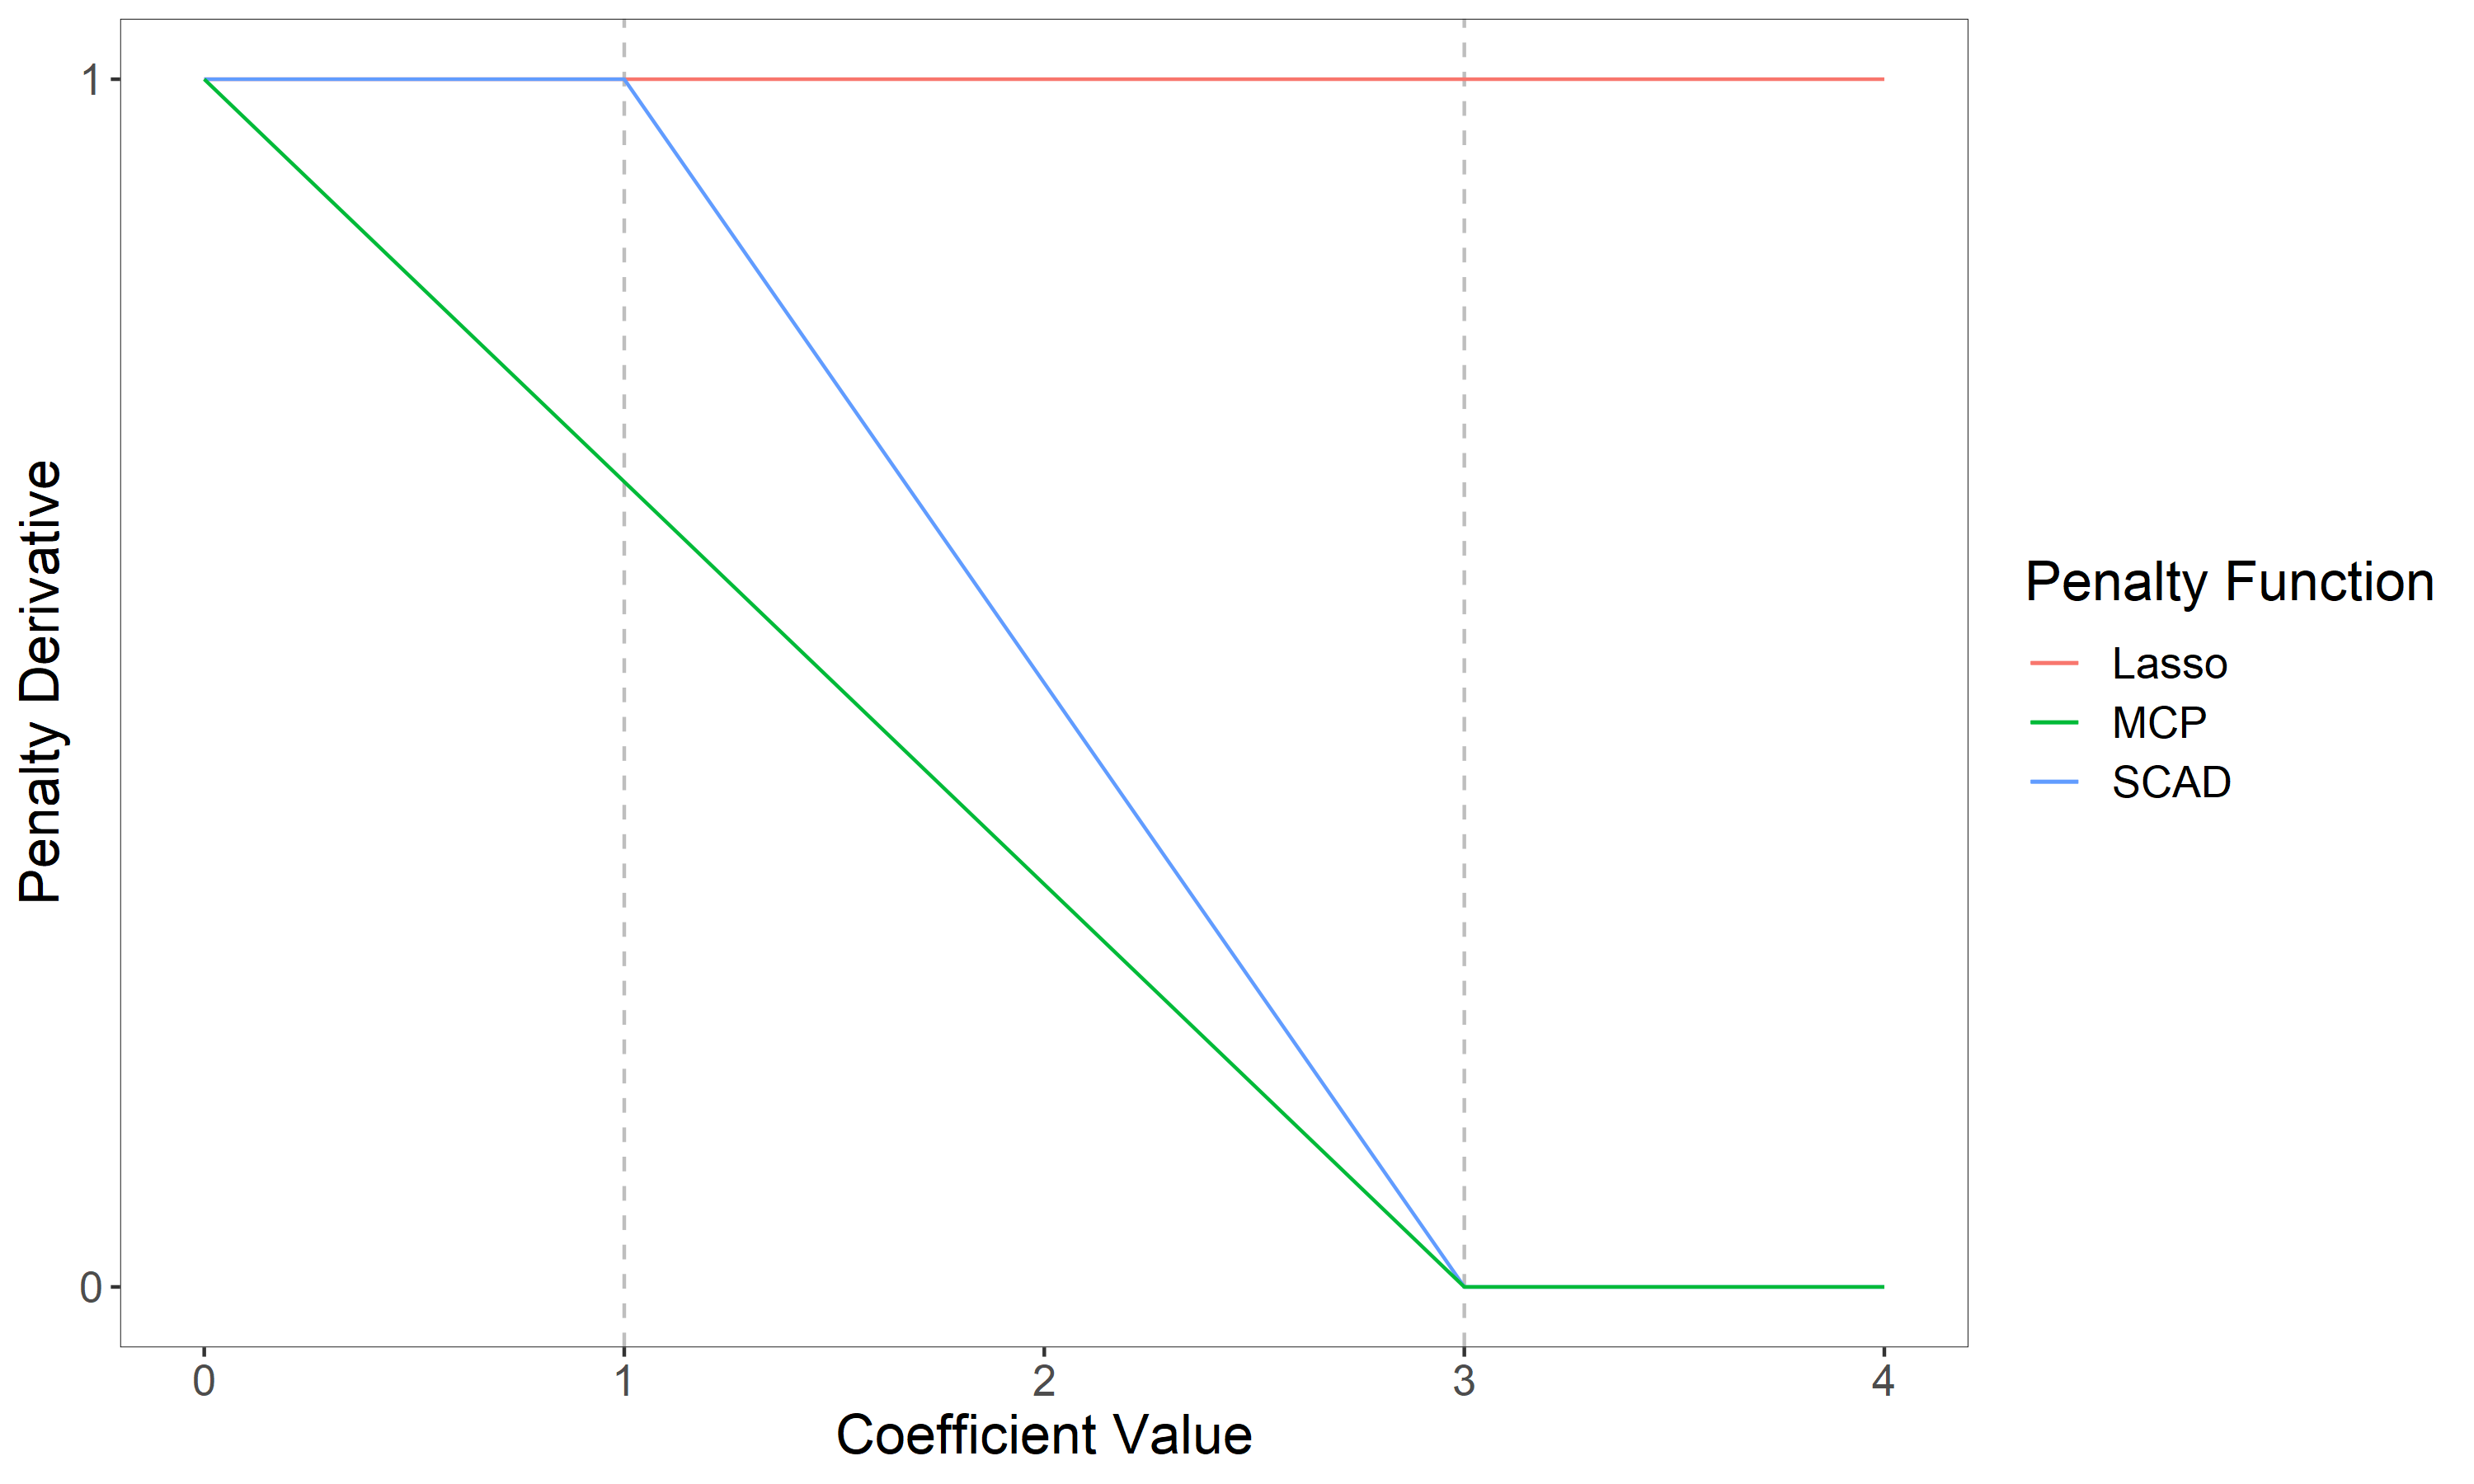
\includegraphics[width=\textwidth]{images/lasso-scad-mcp-derivative.png}
			\captionsetup{width = 0.8\textwidth}
			\caption{Derivatives of the penalty functions for lasso, SCAD, and MCP.}
			\label{fig:derivative}
		\end{subfigure}
		\captionsetup{width = 0.9\textwidth}
		\caption{Penalty functions for lasso, SCAD, and MCP, as well as their derivatives. These plots use $\lambda = 1$ and $a = 3$. The dashed vertical lines are the knots for SCAD and MCP.}
		\label{fig:lasso-scad-mcp}
	\end{figure}
	
	Note that of the penalized regression methods discussed above, only ridge regression has a general closed-form solution. Although lasso, elastic-net, SCAD and MCP do not have closed-form solutions, their solutions can be efficiently approximated \cite{friedman2010regularization, breheny2011ncvreg}. In some special cases, however, a closed-form solution exists. 
	
	Let $\mathbf{X}$ be a $n\times p$ matrix where each row contains the predictor values for one observation. To simplify things, we will assume that our data is centralized so that the coefficient $\beta_0$ is 0; that way, we do not need to include an extra entry of 1 in each row of $\mathbf{X}$. In an \textit{orthonormal design}, we assume that $\mathbf{X}$ is orthonormal, meaning that the magnitude of each column of $\mathbf{X}$ is one and every pair of columns of $\mathbf{X}$ is orthogonal. In this special case, the matrix $(\mathbf{X}^\top \mathbf{X})^{-1}$ is the $p\times p$ identity matrix. As a result, each coefficient is independent of the other coefficients; in other words, we can compute the coefficient estimate for each predictor without needing to use the values for the other predictors. For example, in an orthonormal design, the general solution to ordinary least squares regression given in Equation \ref{eqn:ols-solution} simplifies to
	\begin{equation}\label{ols-orthonormal-solution}
		\hat{\bm{\beta}}^{\text{OLS}} = \mathbf{X}^\top \mathbf{y}
	\end{equation}
	
	To compute the coefficient estimates for lasso, SCAD, and MCP in an orthonormal design, we first compute the vector $\mathbf{z} = \mathbf{X}^\top \mathbf{y}$ \cite{fan2001variable}. Each entry of $\mathbf{z}$ corresponds to one predictor. We then apply a \textit{thresholding function} to each entry of $\mathbf{z}$ to get the coefficient estimate for that predictor. For lasso, elastic-net, SCAD, and MCP, a closed-form for this thresholding function exists \cite{tibshirani1996regression, fan2001variable, zou2005regularization, zhang2010nearly}. The input to the thresholding function is the actual coefficient value, and the output is the estimated value for that coefficient in an orthonormal design. Figure \ref{fig:prediction} shows the threshold functions for lasso, SCAD and MCP when $\lambda = 1$. For SCAD and MCP, we used the value $a = 3$. For reference, the identity line is included, which can be considered as the threshold function for ordinary least squares.
	
	\begin{figure}[!h]
		\centering
		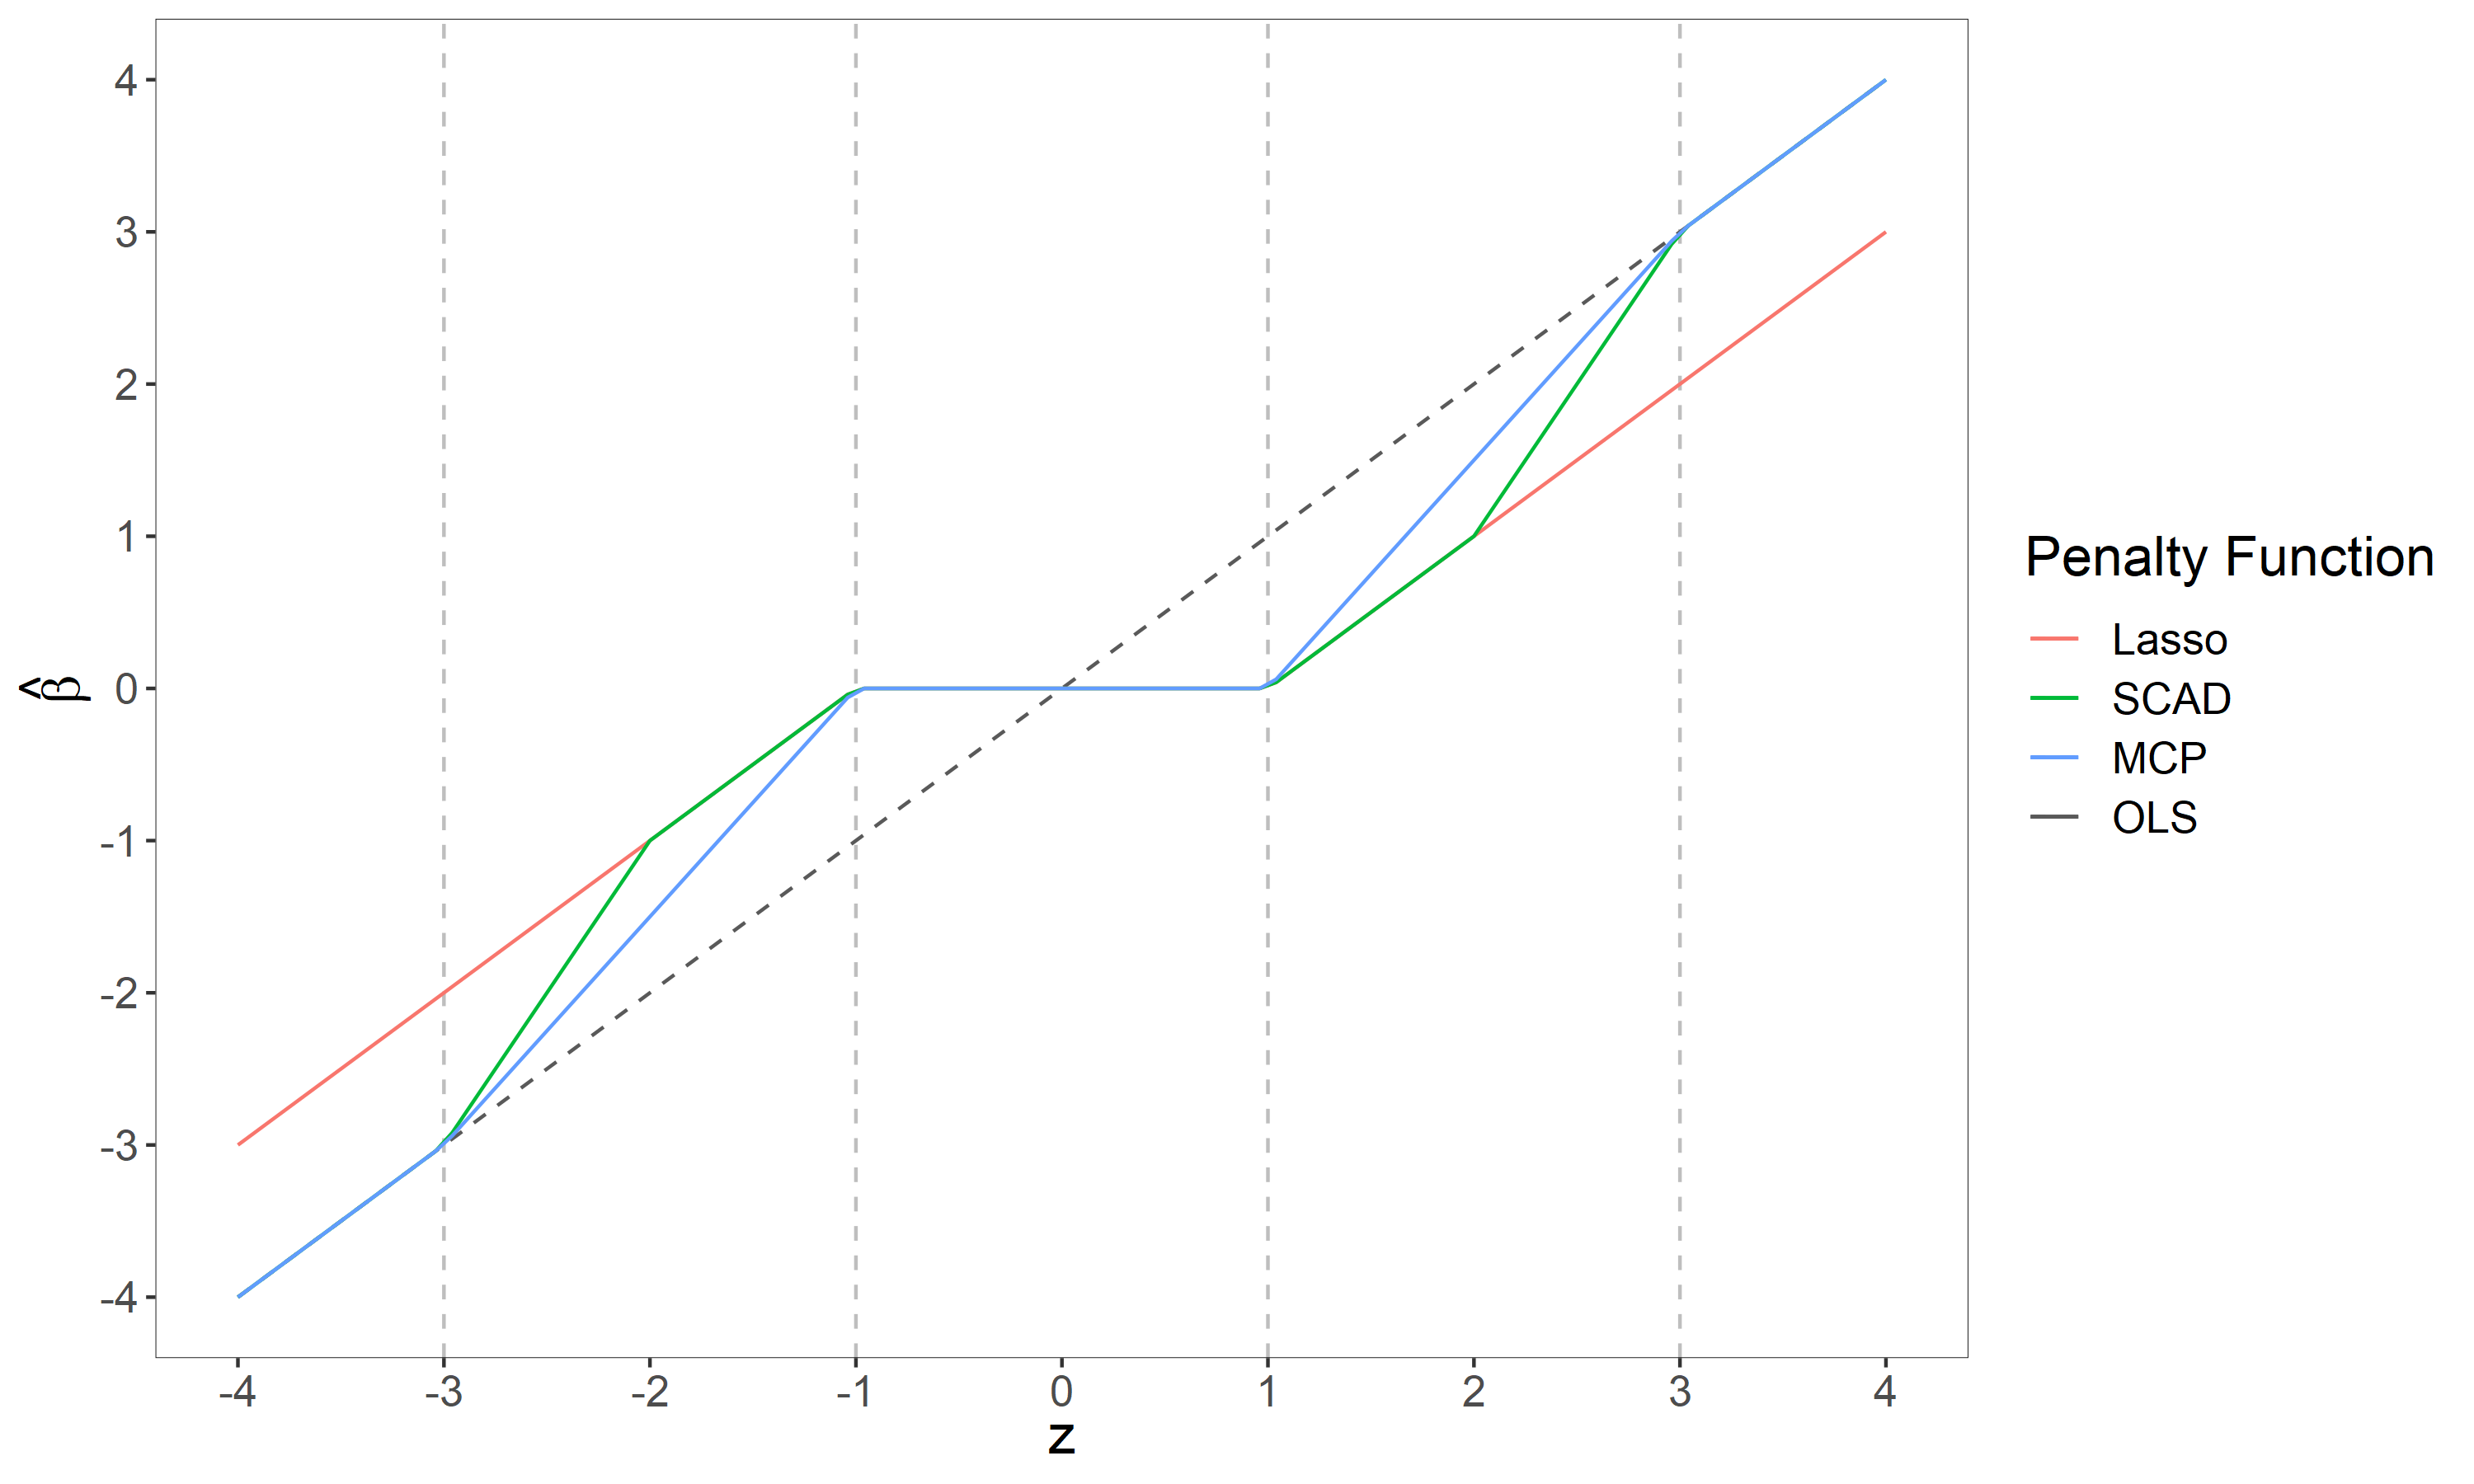
\includegraphics[width = 0.8\textwidth]{images/lasso-scad-mcp-solution.png}
		\captionsetup{width = 0.8\textwidth}
		\caption{Thresholding function for lasso, SCAD, and MCP when $\lambda = 1$ and $a = 3$ in an orthonormal design. The input ($z$) represents an entry from the vector $\mathbf{z}=\mathbf{X}^\top \mathbf{y}$; the output ($\hat{\beta}$) is the coefficient estimate. The dashed vertical lines are the knots for SCAD and MCP.}
		\label{fig:prediction}
	\end{figure}
	
	We see that when $\vert z \vert$ is small, the thresholding function for lasso, SCAD, and MCP are all zero. This matches with the assumption that these methods should set small coefficient estimates to zero. As $\vert z \vert$ increases, the estimated value for that coefficient gets larger. Notice that ordinary least squares doesn't decrease the estimated coefficient value for any choice of $z$; this is because of the fact that ordinary least squares is unbiased, whereas the other methods are biased.
	
	In this figure, we also see that the threshold function for lasso is parallel to the identity line for large values of $\beta$. This means that even if a predictor is very influential on the response, lasso will predict a coefficient estimate that is less than the true coefficient value. This makes lasso a very biased model. This issue was one of the main motivations for SCAD and MCP. Unlike lasso, SCAD and MCP converge to the identity line as $\beta$ increases, which makes these methods less likely to decrease large coefficient estimates.
	\end{comment}
	\begin{comment}
	Another feature of SCAD and MCP is their oracle-like properties \cite{fan2001variable, zhang2010nearly}. The term \textit{oracle} in this context was first proposed by Donohe and Johnstone in \cite{donoho1994ideal}. Suppose that a linear model could be fitted with the aid of an oracle. This oracle could tell you the subset of predictors that are truly related to the response so that a model can be fitted using only the important predictors. Although such a model is not possible in practice, this oracle procedure serves an ideal that can be worked towards.
	
	A linear model is said to have \textit{oracle-like properties} if two asymptotic conditions hold \cite{zou2006adaptive}. Let $p^\ast$ be the number of predictors that have non-zero coefficients. First, as $n\to \infty$, the model must be able to correctly identify the correct subset of non-zero predictors, which we will denote by $\mathcal{A}$. The second condition is that as $n\to\infty$, we must have
	\begin{equation}
		\sqrt{n}(\hat{\bm{\beta}}_\mathcal{A} - \bm{\beta}\mathcal{A})\to_d \mathcal{N}_p^{\ast}(\mathbf{0}, \mathbf{\Sigma}^\ast)
	\end{equation}
	where $\hat{\bm{\beta}}_\mathcal{A}$ are the coefficient estimates for the non-zero predictors, $\bm{\beta}_\mathcal{A}$ are the true coefficient values for the non-zero predictors, and $\mathcal{N}_p^\ast(\mathbf{0}, \mathbf{\Sigma}^\ast)$ is the multivariate normal distribution of the $p^\ast$ non-zero predictors with mean zero and covariance matrix $\mathbf{\Sigma}^\ast$. In other words, as $n\to\infty$, the coefficient estimates for the non-zero predictors is normally distributed around the true coefficient values. Importantly, this means that the expected value for the coefficient estimates are the true coefficient values.
	
	Both SCAD and MCP have oracle-like properties under certain conditions \cite{fan2001variable, zhang2010nearly}. Hence, SCAD and MCP can perform as well as the oracle estimator as $n$ approaches $\infty$. On the other hand, lasso does not have oracle-like properties, meaning that its predictions cannot perform as well as a model found with the aid of an oracle.
	\end{comment}
	Another feature of SCAD and MCP is their oracle-like properties \cite{fan2001variable, zhang2010nearly}. This means that as $n\to\infty$, SCAD and MCP will correctly identify exactly which predictors should have non-zero coefficients, and that the coefficient estimates will be normally distributed with the mean estimate being the true coefficient value \cite{zou2006adaptive}.
	
	\subsection{Non-linear models}
	We next discuss several non-linear methods for regression: random forests, gradient boosting, and support vector machines.
	
	\begin{comment}
	Both random forest and gradient boosting models use \textit{decision trees} to make predictions. A decision tree is a binary tree where each non-leaf node represents a condition and each leaf node represents a prediction value. To make a prediction, start at the root node and check whether the condition at that node is true or false. If true, move down to the node's first child; if false, move to the second child. This process is repeated until a leaf node is reached. This node will give a value that the decision tree predicts. Figure \ref{fig:decision-tree} gives an example of a decision tree with regression.
	
	\begin{figure}[h!]
		\centering
		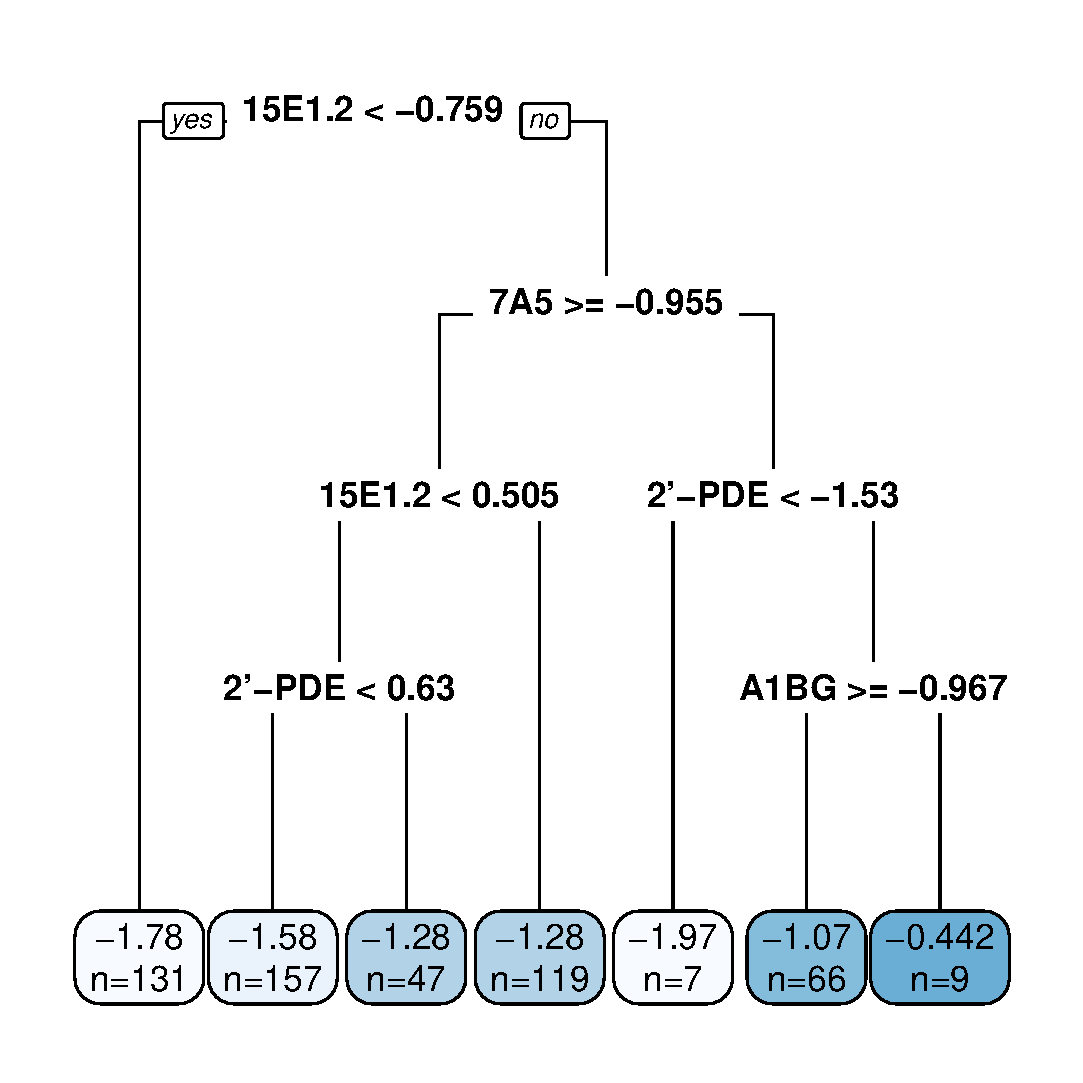
\includegraphics[width = 0.4\textwidth]{images/decision-tree.eps}
		\captionsetup{width = 0.8\textwidth}
		\caption{Example of a decision tree. This tree was generated using a \lstinline!brTCGA! data set \cite{zeng2017biglasso}. It attempts to predict the gene expression of the BRCA1 gene based on the expression of other genes. The decision tree was fitted and plotted with the \lstinline!rpart! and \lstinline!rpart.plot! libraries in \lstinline!R!.}
		\label{fig:decision-tree}
	\end{figure}
	
	Although decision trees can be used as machine learning models on their own, it is more common to use decision trees in \textit{ensemble methods}, which combine many different decision trees into a single model. This is because a single decision tree will usually have high variance since a small change in the training set can lead to a completely different decision tree \cite{james2013introduction}.
	\end{comment}
	
	\begin{comment}
	\textit{Random Forests} (RF) solve the issue of high variance by aggregating the predictions of many independent decision trees \cite{breiman2001random}. Each tree is fit using a subset of the observations and a subset of the predictors so that the trees are relatively independent from one another.
	
	To fit each decision tree within a random forest model, we first select a random sample of the $n$ observations with replacement, in a process called \textit{bootstrapping} \cite{efron1994introduction}. The number of observations chosen for each tree is a hyperparameter that can be changed. After selecting a set of observations, a random sample of predictors are chosen out of the $p$ predictors without replacement. Again, this helps decorrelate the trees. The number of predictors used in each tree is also a hyperparameter that can be changed. A decision tree is then generated using the available observations and predictors.
	
	A random forest model aggregates all of the individual decision trees into a single model. The number of trees generated, $B$, is a hyperparameter that can be changed; usually, a random forest model will contain at least several hundred trees. To make predictions with a random forest, a test observation is passed into each decision tree and the predictions from each tree are aggregated. Figure \ref{fig:random-forest} demonstrates how a prediction is made using a random forest. For regression, the results are normally aggregated using the mean; for classification, the prediction chosen most often by the trees is usually used as the final prediction. 
	
	\begin{figure}[h!]
		\footnotesize
		\centering
		\begin{forest}
	[Test observation,inner sep = 0.2cm, rounded corners, minimum height = 0.6cm, draw = black, fill = cyan!20
		%Tree 1
		[,circle,draw,fill=cyan,edge={->},label=Tree 1
			[,circle,draw,fill=cyan
				[,circle,draw
					[,circle,draw]
					[,circle,draw]
				]
				[,circle,draw,fill=cyan
					[,circle,draw]
					[,circle,draw,fill=cyan
						[Prediction 1,edge={->},inner sep = 0.2cm, rounded corners, minimum height = 0.6cm, draw = black, fill = green!20] {
							\draw[->] () to (agg);
						}
					]
				]
			]
			[,circle,draw
				[,circle,draw
					[,circle,draw]
					[,circle,draw]
			]
				[,circle,draw
					[,circle,draw]
					[,circle,draw]
				]
			]
		]
		% Tree 2
		[,circle,draw,fill=cyan,edge={->},label={[xshift=-2em,font=\small]Tree 2}
			[,circle,draw
				[,circle,draw
					[,circle,draw]
					[,circle,draw]
				]
				[,circle,draw
					[,circle,draw]
					[,circle,draw]
				]
			]
			[,circle,draw,fill=cyan
				[,circle,draw,fill=cyan
					[,circle,draw]
					[,circle,draw,fill=cyan
						[Prediction 2,edge={->},inner sep = 0.2cm, rounded corners, minimum height = 0.6cm, draw = black, fill = green!20
							[Aggregate result,edge={->},inner sep = 0.2cm, rounded corners, minimum height = 0.6cm, draw = black, fill = cyan!20,name=agg]
						]
					]
				]
				[,circle,draw
					[,circle,draw]
					[,circle,draw]
				]
			]
		]
		[..., l*=2,edge={->},inner sep = 0.2cm, rounded corners, minimum height = 0.6cm, draw = black, fill = cyan!20
			[...,l*=3,edge={->},inner sep = 0.2cm, rounded corners, minimum height = 0.6cm, draw = black, fill = green!20] {
			\draw[->] () to (agg);
			}
		]
		% Tree 3
		[,circle,draw,fill=cyan,edge={->},label=Tree $B$
			[,circle,draw
				[,circle,draw
					[,circle,draw]
					[,circle,draw]
				]
				[,circle,draw
					[,circle,draw]
					[,circle,draw]
				]
			]
			[,circle,draw,fill=cyan
				[,circle,draw
					[,circle,draw]
					[,circle,draw]
				]
				[,circle,draw,fill=cyan
					[,circle,draw]
					[,circle,draw,fill=cyan
						[Prediction $B$,edge={->},inner sep = 0.2cm, rounded corners, minimum height = 0.6cm, draw = black, fill = green!20] {
							\draw[->] () to (agg);
						}
					]
				]
			]
		]
	]
\end{forest}
		\captionsetup{width = 0.8\textwidth}
		\caption{Visualization of how predictions are made using a random forest model. An observation is input into each decision tree. Predictions from each tree are then aggregated into a single result that is used as the final prediction.}
		\label{fig:random-forest}
	\end{figure}
	\end{comment}
	
	A \textit{random forest model} aggregate the predictions of a large ensemble of decision trees to estimate the response value \cite{breiman2001random}. Each tree is fitted independently using a subset of predictors and observations. The observations are selected \textit{with replacement}, in a process called \textit{bootstrapping} \cite{efron1994introduction}.
	
	\begin{comment}
	This idea of fitting multiple models with bootstrapping and aggregating the results can be used with other models besides decision trees. In general, this process is called \textit{bagging} (a combination of the words ``bootstrap'' and ``aggregating'') \cite{breiman1996bagging}. 
	\end{comment}
	
	
	\begin{comment}
	\textit{Boosting} is the technique of sequentially improving a weak learner until it becomes a strong learner \cite{schapire1990strength}. A \textit{gradient boosting machine} (GBM) is a boosting technique that uses gradient descent to minimize error in a model and correct the shortcomings of the previous model \cite{friedman2001greedy}. Boosting can be used on different types of models, but decision trees are the most common to use. Unlike random forest models, where each tree is independent of one another, the trees in a boosting model are grown sequentially. Each tree is fitted to correct the mistakes made by the previous tree. The details of how errors are corrected depends on the algorithm selected. With regression, each tree can be fitted by using the residuals from the previous tree as the training data \cite{james2013introduction}. Like random forest models, predictions are made by aggregating the results from each individual tree. See figure \ref{fig:boosting} for a diagram of how a boosting model is fitted.
	
	\begin{figure}[b!]
		\footnotesize
		\centering
		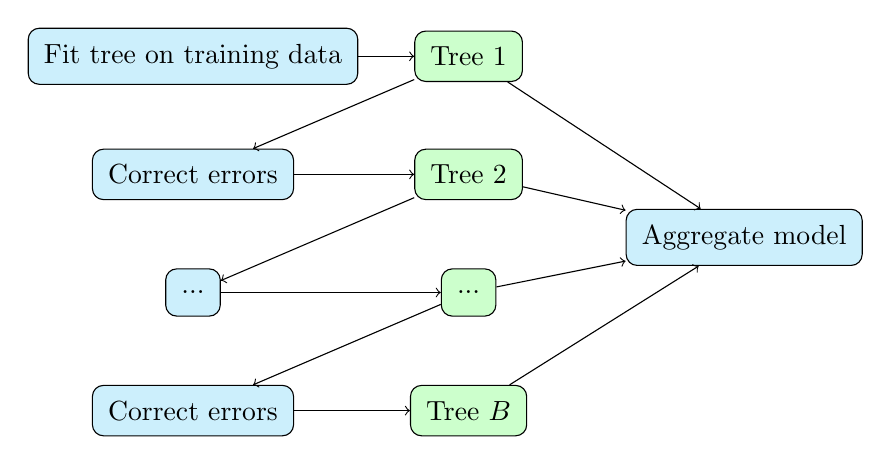
\begin{tikzpicture}
	\node (fit1)[fit]{Fit tree on training data};
	\node (tree1)[tree, right of = fit1, xshift = 2.5cm]{Tree 1};
	\node (fit2)[fit, below of = fit1, yshift = -0.5cm]{Correct errors};
	\node (tree2)[tree, right of = fit2, xshift = 2.5cm]{Tree 2};
	\node (fit3)[fit, below of = fit2, yshift = -0.5cm]{...};
	\node (tree3)[tree, right of = fit3, xshift = 2.5cm]{...};
	\node (fit4)[fit, below of = fit3, yshift = -0.5cm]{Correct errors};
	\node (tree4)[tree, right of = fit4, xshift = 2.5cm]{Tree $B$};
	\node (end)[fit, right of = tree2, xshift = 2.5cm, yshift = -0.8cm]{Aggregate model};
	
	\draw [->] (fit1) -- (tree1);
	\draw [->] (tree1) -- (fit2);
	\draw [->] (fit2) -- (tree2);
	\draw [->] (tree2) -- (fit3);
	\draw [->] (fit3) -- (tree3);
	\draw [->] (tree3) -- (fit4);
	\draw [->] (fit4) -- (tree4);
	
	\draw [->] (tree1) -- (end);
	\draw [->] (tree2) -- (end);
	\draw [->] (tree3) -- (end);
	\draw [->] (tree4) -- (end);
\end{tikzpicture}
		\captionsetup{width = 0.8\textwidth}
		\caption{How a boosting model with decision trees is fitted. Each tree is fitted to correct the errors of the previous tree. Predictions are made by combining the results from each decision tree.}
		\label{fig:boosting}
	\end{figure}
	
	Gradient boosting machines that use decision trees can be used for both regression and classification. When using a gradient boosting model with decision trees, \textit{relative variable importance} and \textit{pruning} can be used as a sort of pseudo-variable selection method to lower complexity and prevent over-fitting. However, this does not yield the same interpretability or bias trade off benefits that true variable selection yields. When using a gradient boosting model with linear regression, there is the ability to use lasso, ridge, and elastic net penalized regression as the weak learner and perform variable selection, although this is much less commonly used than decision trees in gradient boosting.
	
	Gradient boosting models often suffer from slow computation speeds due to the large number of sequential models that need to be trained. \textit{Extreme Gradient Boosting} (XGBoost) is a faster version of gradient boosting that utilizes parallel computing as well as different optimization techniques to speed up computation \cite{chen2016xgboost}. For these reasons, XGBoost is often preferred over standard gradient boosting models and is very commonly used in many machine learning applications. In this study, we will use the XGBoost algorithm for gradient boosting.
	
	There are a few different hyperparameters that can control how an XGBoost model is fit. The learning rate controls how quickly the gradient boosting model learns. If this learning rate is high, then the model learns quickly, but it may not learn as efficiently. If the learning rate is low, then the model takes longer but typically makes better predictions. The maximum tree depth determines how high each tree can be. Using smaller tree sizes may oversimplify the model, but it could also mitigate overfitting.
	\end{comment}
	\textit{Boosting} is the technique of sequentially improving a weak learner until it becomes a strong learner \cite{schapire1990strength}. A \textit{gradient boosting machine} (GBM) is a boosting technique that uses gradient descent to minimize error in a model and correct the shortcomings of the previous model \cite{friedman2001greedy}. Unlike random forest models, where each tree is independent of one another, the trees in a boosting model are fitted sequentially to correct the mistakes made by the previous tree.
	
	\begin{comment}
	The final non-linear model that we considered is the \textit{support vector machine} (SVM) \cite{cortes1995support}. Support vector machines are versatile models that can be used for both classification and regression. Originally, a support vector machine was designed as a binary classifier that separates the two response classes with a hyperplane in $(p - 1)$-dimensional space. The hyperplane chosen by a support vector machine is chosen to maximize the distance between the hyperplane and any of the observation points. The observations closest to this separating hyperplane are called \textit{support vectors}. Predictions are made by determining which side of the hyperplane an observation lies on. Observations that lie above the hyperplane are assigned to one class, and observations on the other side are predicted to be the other class. Figure \ref{fig:svm} demonstrates a simple support vector machine for classification.
	
	\begin{figure}[h!]
		\centering
		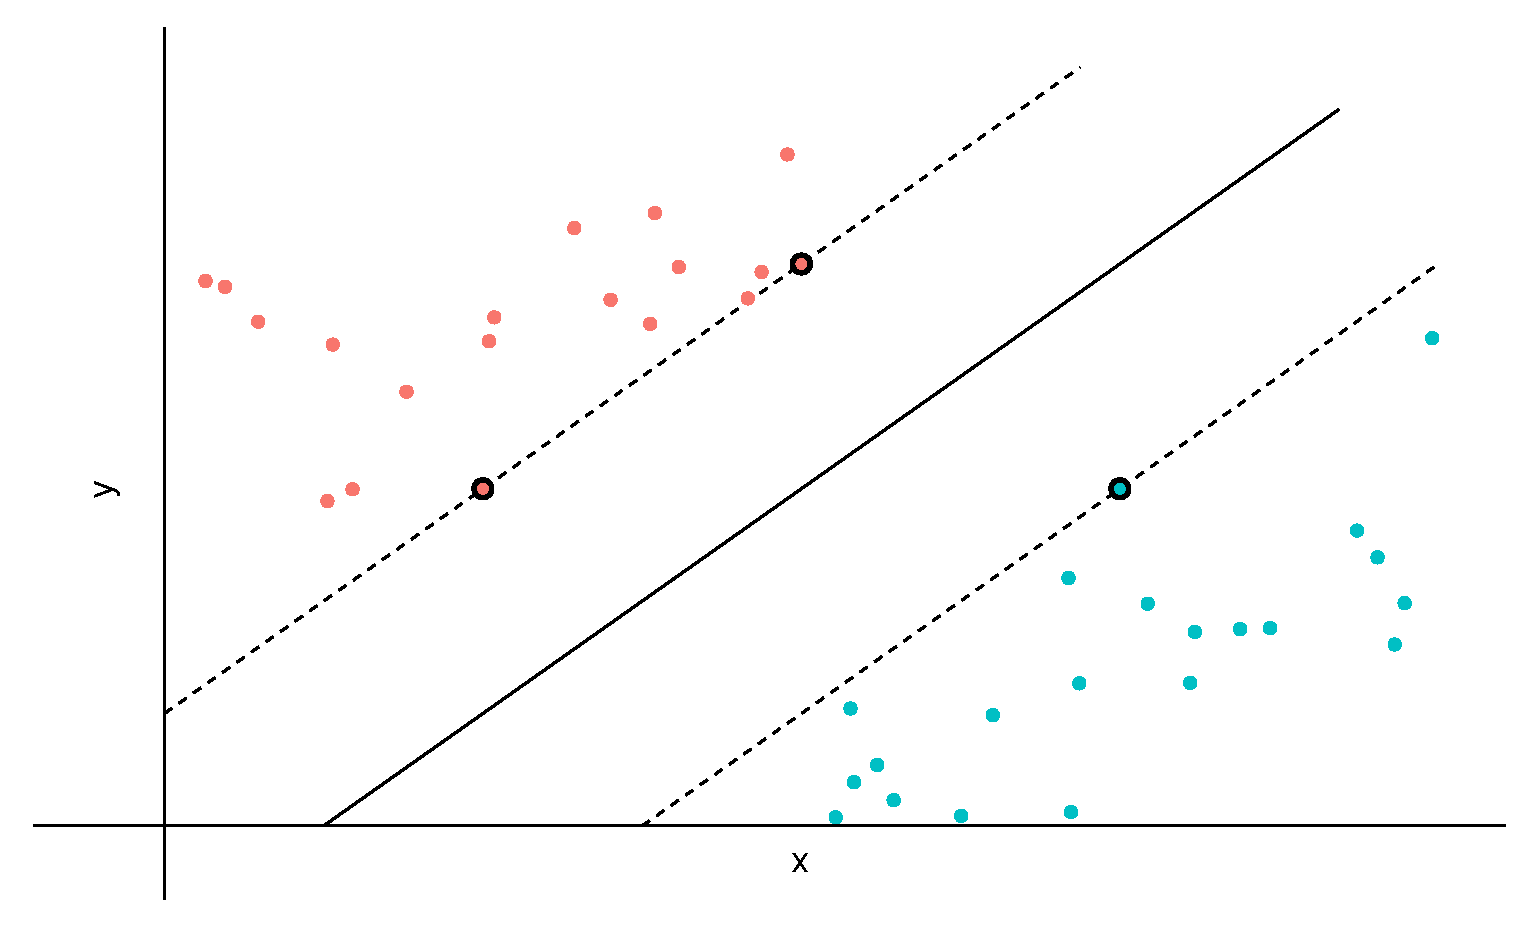
\includegraphics[width = 0.8\textwidth]{images/svm.eps}
		\captionsetup{width = 0.8\textwidth}
		\caption{Visualization of a simple support vector machine for binary classification. The solid black line is the hyperplane that maximizes the margin between the two classes. The points with a black outline are the support vectors. They are the points that define the hyperplane.}
		\label{fig:svm}
	\end{figure}
	
	Note that in most data sets, the classes cannot be split perfectly into two sides. Furthermore, this model has very high variance as changing the points near the hyperplane can significantly alter the hyperplane. Finally, this model cannot handle cases where the true boundary is non-linear. Luckily, support vector machines in practice can handle such issues. Typically, support vector machines are allowed to misclassify some of the training data, which address the cases where the data cannot be split perfectly by a hyperplane. Also, the predictor space can be enlarged to handle non-linear decision boundaries; this is typically done by using \textit{kernels}. For example, using a radial kernel can create decision boundaries that enclose regions of the $p$-dimensional space.
	
	Support vector machines can also be generalized to handle classification when there are more than two classes. They can also be used for regression \cite{drucker1997support}. We will be using support vector machines for regression in our study.
	
	Like the other non-linear methods, there are many different hyperparameters that can be tuned. The two hyperparameters that we considered are $\epsilon$ and the cost function. The hyperparameter $\epsilon$ defines how tolerant the algorithm is of small errors. If $\epsilon$ is large, then the support vector machine will tolerate larger errors; if $\epsilon$ is small, then even small errors will be punished. The cost hyperparameter $C$ determines how strongly the model punishes incorrect predictions. If $C$ is large, then the model punishes incorrect predictions more, making it fit more tightly to the training set. If $C$ is smaller, then the model is likely to allow more incorrect predictions in the training data.
	\end{comment}
	The final non-linear model that we considered is the \textit{support vector machine} (SVM) \cite{cortes1995support, drucker1997support}. Support vector machines find a hyperplane that closely fits the data. Unlike linear regression, support vector machines can address non-linear relationships between the response and its predictors.
	
	%%%%%%%%%%%%%%%%%%%%%%%%%%%%%%%%%%%%%%%%%%%%%%%%%%%%%%%%%%%%%%%%%%%%%
	%\section{Methods}
	%To test and evaluate each of the models discussed above, we considered both Monte Carlo simulations and empirical data. Monte Carlo simulations allow us to test the models under different environments to get a comprehensive idea of how each model performs. Furthermore, by repeating each simulation many times, our results will be more consistent than if we just relied on one data set to test each model.
	
	\subsection{Implementation}
	% lists and describes every tested model. Can include equations for models, but should not go into such great depth about each model: that can be reserved for literature review portion of the paper.
	
	This section gives the specific details how we fit each model for both the simulated data and the empirical data.
	\begin{comment}
	All of our simulations were run using version 4.1.0 of \lstinline!R!. Several different libraries were used to fit machine learning models using our simulated data. Table \ref{tab:model-libraries} summarizes the libraries used to fit models.
	\end{comment}
	 Everything in our study was run on version 4.1.0 of \lstinline!R! \cite{r}. Table \ref{tab:model-libraries} summarizes the packages used for each model.
	 
	\begin{table}[h]
		\centering
		\caption{\lstinline!R! Libraries used and the models used from each library}
		\label{tab:model-libraries}
		\begin{tabular}{lll}\hline
			\textbf{Library}    	  & \textbf{Models used}                                 & \textbf{Version} \\ \hline
			\lstinline!stats! \cite{r}   	  & Ordinary least squares                               & 4.1.0            \\
			\lstinline!MASS! \cite{venables2002mass}   	  & Forward and backward selection                       & 7.3-54           \\
			\lstinline!glmnet! \cite{friedman2010regularization} 	  & Ridge, lasso, elastic-net                            & 4.1-1            \\
			\lstinline!ncvreg! \cite{breheny2011ncvreg}	      & SCAD and MCP                                         & 3.13.0           \\
			\lstinline!xgboost! \cite{chen2021xgboost}	  & Gradient boosting                                    & 1.4.1.1          \\
			\lstinline!ranger! \cite{wright2017ranger} 	  & Random forest (simulations)                          & 0.12.1           \\
			\lstinline!randomForest! \cite{liaw2002rf} & Random forest (empirical data)                       & 4.6-14           \\
			\lstinline!e1071! \cite{meyer2021e1071}  	  & Support vector machine                               & 1.7-7            \\\hline
		\end{tabular}
	\end{table}
	
	Ordinary least squares models were fitted using the \lstinline!lm! function from the \lstinline!stats! package in base \lstinline!R!.
	
	Subset selection models using forward, backward, stepwise forward, and stepwise backward selections were fitted using the \lstinline!MASS! library. For each of these four algorithms, we fit models using two criteria that determine when to stop adding and removing predictors: Akaike Information Criterion (AIC) and Bayesian Information Criterion (BIC) \cite{akaike1998information, schwarz1978estimating}. In general, using the AIC will lead to more predictors getting non-zero coefficient estimates.
	
	Ridge, lasso, and elastic-net models were fitted using \lstinline!glmnet!. We used the \lstinline!cv.glmnet! function, which uses cross validation grid search to determine the value of $\lambda$ that minimizes the cross validation error. Using cross validation can help generate a model that performs well on both training and testing data. We used the default value of 10 folds to fit models using \lstinline!glmnet!. For elastic-net regression, we used the hyperparameter $\alpha = 0.8$ in our simulation study. This means that the elastic-net model has a stronger lasso penalty and a weaker ridge penalty. This value of $\alpha$ was chosen so that the elastic-net model could emphasize the variable selection provided by lasso while also allowing it to handle multicollinearity from ridge. For the empirical data analysis, we instead used $\alpha = 0.5$. The remaining hyperparameters were given their default values.
	
	For SCAD and MCP models, we used the \lstinline!cv.ncvreg! function from the \lstinline!ncvreg! library. Both SCAD and MCP depend on an additional hyperparameter $a$. We used the default values of $a$ for both models: 3 for MCP and 3.7 for SCAD (note that the \lstinline!ncvreg! documentation calls this hyperparameter $\gamma$ instead of $a$). All other arguments were given their default values. 
	%%%%  Why did we use these values??
	
	For the three non-linear models (gradient boosting, random forests, and support vector machines), we used cross validation and grid search to find suitable hyperparameters, and then fit a model using the full training set using the hyperparameters selected. Because many of the data sets used had large values of $n$ and $p$, only a few hyperparameters were tuned. This ensured that the models could be fit within a reasonable amount of time. All other hyperparameters were given their default values.
	
	For gradient boosting with \lstinline!xgboost!, we used different values for the learning rate (0.1, 0.3, and 0.5) and maximum tree depth (1, 3, and 7). A maximum of 1000 trees were generated, with an early stopping condition if the model failed to improve for 10 iterations in a row. We used five folds in the cross validation.
	
	For random forests, we used \lstinline!ranger! for the simulated data and \lstinline!randomForest! for the empirical data. We did not use \lstinline!ranger! for the empirical data because it could not handle the large number of predictors, resulting in stack overflow errors. For both \lstinline!ranger! and \lstinline!randomForest!, we tuned the number of predictors used per decision tree ($\lfloor \sqrt{p}\rfloor$, $\lfloor p / 3 \rfloor$, and $\lfloor p / 2 \rfloor$) and the number of trees (300, 400, 500 and 600). The best model was selected based on the out-of-bag error, which represents the average error for each observation using only the trees that did not include that observation.
	
	Finally, for support vector machines using \lstinline!e1071!, we varied $\epsilon$ (0.1, 0.5, 2), which affects the model's sensitivity to small errors. We also controlled the cost value $C$ (0.5, 1, 2), which affects how much the model punishes wrong predictions.
	
	Some of the models used could only be used for certain values of $n$ and $p$. This is because either the runtime becomes unreasonable when $n$ or $p$ are large, or the model simply cannot be used when $p$ is too large. Ordinary least squares was only used when $p\leq n$, since it cannot be used at all when $p>n$. For the same reason, the backward subset selection algorithms were also used only when $p\leq n$. The forward subset selection algorithms were only used when $p\leq n$ and $p\leq 40$. When $p>40$, the runtimes for forward selection and forward stepwise selection become unreasonably long due to the exponentially increasing number of possible predictor combinations.
	
	Lasso, SCAD, MCP, GBM, and random forest models were used for all data sets. Support vector machine models were made for all of the simulated data but was not used for the empirical data. Support vector machine models cannot handle the immense number of predictors in our empirical data.
	
	\section{Monte Carlo Simulations}\label{sec:simulations}
	% outline data generation process and factorial design process
	
	\textit{Monte Carlo simulations} use randomly generated data to fit and test regression  models. There are several benefits to using simulated data rather than experimental data. For one, the true relationship between the predictor variables and the response is known. Simulations can also be iterated many times, giving sturdier results about the effectiveness of each model. Finally, Monte Carlo simulations give us full control over how our data is distributed. This enables us to evaluate the models under various conditions.
	
	
	\subsection{Simulation Design}
	
	Our simulation study used two different functions for the response variable $Y$. Our first function assumed a linear relationship between the response and its predictors $X_1, X_2, \dotsc, X_p$, while the second response used a non-linear relationship. By considering both linear and non-linear response functions, we obtain a more thorough understanding of how each model performs in different situations.
	
	\begin{comment}
	With our linear response function, we assumed that
	\begin{equation}
		Y = \beta_0 + \beta_1 X_1 + \cdots + \beta_p X_p + \epsilon
	\end{equation}
	where $\beta_0$ is some intercept, $\beta_1, \dotsc, \beta_p$ are coefficient values and $\epsilon\sim \mathcal{N}(0, \sigma^2)$ is a normally distributed random error with mean 0 and variance $\sigma^2$. We chose the values $\beta_0 = 1$, $\beta_1 = 2$, $\beta_2 = -2$, $\beta_5=0.5$ and $\beta_6 = 3$, while the remaining coefficient values were set to 0.
	
	To generate the data, we first defined $\bm{\beta} = [\beta_0, \beta_1, \dotsc, \beta_p]^\top$, a $(p + 1)\times 1$ vector of coefficient values. Next, we generated $\mathbf{X}$, a $n\times (p + 1)$ matrix where each row contains the predictor values for one observation with an extra value of 1 in the first entry. The entries for the remaining columns of $\mathbf{X}$ were generated using the $p$-dimensional multivariate normal distribution $\mathcal{N}_p(0, \mathbf{\Sigma})$ with mean zero and covariance matrix $\mathbf{\Sigma}$. We assumed that every predictor had a standard deviation of 1, making the covariance matrix equivalent to a correlation matrix. Four different correlation matrix structures were considered in our study, which are discussed later.
	
	We then generated an $n\times 1$ error vector $\mathbf{e}\sim \mathcal{N}(0, \sigma^2)$ with mean zero and variance $\sigma^2$. The response $\mathbf{y}$ can then be computed by
	\begin{equation}
		\mathbf{y} = \mathbf{X}\bm{\beta} + \mathbf{e}
	\end{equation}
	
	Given our chosen coefficient values, the response $\mathbf{y}$ becomes
	\begin{equation}\label{eqn:linear-response}
		\mathbf{y} = 1 + 2\mathbf{X}_1 - 2\mathbf{X}_2 + 0.5\mathbf{X}_5 + 3\mathbf{X}_6 + \mathbf{e}
	\end{equation}
	where $\mathbf{X}_i$ is the $i$-th column of $\mathbf{X}$.
	
	Our second response function calculated $\mathbf{y}$ as
	\begin{equation}\label{eqn:nonlinear-response}
		\mathbf{y} = 6\times 1_{\mathbf{X}_1>0} + \mathbf{X}_2^2 + 0.5\mathbf{X}_6 + 3\mathbf{X}_7 + 2\times 1_{\mathbf{X}_8>0}\times 1_{\mathbf{X}_9>0} + \mathbf{e}
	\end{equation}
	where $1_{\mathbf{X}_i>0}$ is the index function defined by
	\begin{equation}
		1_{\mathbf{X}_i>0} = \left\{\begin{array}{ll}
			0, &\mathbf{X}_i \leq 0 \\
			1, &\mathbf{X}_i > 0
		\end{array}\right.
	\end{equation}
	Note that this response function does have linear terms, but the function as a whole is non-linear.
	\end{comment}
	
	The linear response function assumes that
	\begin{equation}\label{eqn:linear-response}
		Y = 1 + 2X_i - 2X_2 + 0.5X_5 + 3X_6 + \epsilon
	\end{equation}
	where $\epsilon$ is an independent random error with mean 0 and constant variance. We refer to this linear response function as Model 1. Our non-linear response function uses
	\begin{equation}\label{eqn:nonlinear-response}
		Y = 6\times 1_{X_1 > 0} + X_2^2 + 0.5X_6 + 3X_7 + 2\times 1_{X_8 > 0}\times 1_{X_9>0} + \epsilon
	\end{equation}
	where $1_{X_i>0}$ is the index function given by
	\begin{equation}
		1_{X_i > 0} = \left\{\begin{array}{rl}
			0, & X_i \leq 0 \\
			1, & X_i > 0
		\end{array}\right.
	\end{equation}
	Note that the non-linear response still includes linear terms. We refer to this non-linear response function as model 2.
	
	For each simulation, we generated a random $n\times (p + 1)$ matrix $\mathbf{X}\sim \mathcal{N}_p(0, \mathbf{\Sigma})$, where $\mathcal{N}_p(0, \mathbf{\Sigma})$ is the multivariate normal distribution with mean zero and covariance matrix $\Sigma$. The response $\mathbf{y}$ was then computed using one of the response functions. Finally, a normally distributed random error $\mathbf{e}\sim \mathcal{N}(0, \sigma^2)$ with mean 0 and standard deviation $\sigma$ was added to the response.
	
	We assumed that the variance for each predictor was 1, meaning that the covariance matrix $\mathbf{\Sigma}$ is actually a correlation matrix. For any $i \neq j$, the entry $\mathbf{\Sigma}_{ij}$ represents the correlation between predictors $i$ and $j$. Correlation between predictors can affect the ability for models to identify important predictors and make accurate predictions.
	
	We considered the following correlation structures for our simulation study:
	\begin{itemize}\itemsep0pt
		\item \textit{Independent} correlation, where $\mathbf{\Sigma} = \mathbf{I}_p$, the $p\times p$ identity matrix;
		\item \textit{Symmetric compound} correlation, where $\mathbf{\Sigma}_{ij} = \rho \in (0, 1)$ for all $i \neq j$;
		\item \textit{Autoregressive correlation}, where $\mathbf{\Sigma}_{ij} = \rho^{\vert i - j \vert}$, where $\rho \in (0, 1)$; and
		\item \textit{Blockwise correlation}, where $\mathbf{\Sigma}$ is block diagonal with each block having symmetric compound structure (and a shared value of $\rho$)
	\end{itemize}
	
	\begin{comment}
	Our simulation study used a \textit{factorial design}. This means that we considered several factors that affect the simulated data in $\mathbf{X}$, each having multiple possible values. We then generated data using every possible combination of factor values, giving us a comprehensive assessment of model performance under various conditions. The factors that we controlled in our simulation are:
	\end{comment}
	
	Our simulation study uses a \textit{factorial design}, meaning that we ran simulations using every possible combination of different factors. The factors that we varied in our simulation study are
	\begin{itemize}\itemsep0pt
		\item The choice of response function (linear or non-linear)
		\item $n$, the number of observations (50, 200, and 1000),
		\item $p$, the number of predictors (10, 100, and 2000),
		\item $\sigma$, the standard deviation of the random error (1, 3, and 6),
		\item The correlation matrix structure (independent, symmetric compound, autoregressive, and blockwise), and
		\item $\rho$, the correlation between predictors (0.2, 0.5, and 0.9)
	\end{itemize}
	
	By taking every possible combination of these factors, we obtain $2\times 3\times 3\times 3\times 4\times 3 = 648$ different settings for the simulations. However, because an independent correlation matrix does not have any correlation between predictors, the value of $\rho$ is not used. Hence, we only needed to run 540 different settings. For each combination of factors, we ran 100 simulations. Each simulation randomly generated two data sets: one to train the various models, and one to test the models and evaluate performance. Both data sets contained $n$ observations, meaning that a total of $2n$ observations were generated for each simulation.
	
	\begin{comment}
	As mentioned earlier, we considered four different covariance matrix structures. These structures determine the correlation between different predictors. If $\mathbf{\Sigma}$ is a correlation matrix, then $\mathbf{\Sigma}_{ij}$ (the entry at the $i$-th row and $j$-th column) represents the correlation between predictors $i$ and $j$. If $\mathbf{\Sigma}_{ij}=0$, there is no correlation; but if $\mathbf{\Sigma}_{ij}=1$, then predictors $i$ and $j$ are perfectly correlated. Note that a correlation matrix is always symmetric, so $\mathbf{\Sigma}_{ij} = \mathbf{\Sigma}_{ji}$ for all indices $i$ and $j$. This correlation can severely impact the performance of statistical models; if several predictors are highly correlated, then we expect the models to be less able to determine which predictors are actually related to the response.
	
	The first correlation structure we considered is \textit{independent correlation}. This means that the correlation matrix $\mathbf{\Sigma}$ has the form
	\begin{equation}
		\mathbf{\Sigma} = \begin{bmatrix}
			1 & 0 & \cdots & 0 \\
			0 & 1 & \cdots & 0 \\
			\vdots & \vdots & \ddots & \vdots \\
			0 & 0 & \cdots & 1
		\end{bmatrix}
	\end{equation}
	In other words, there is no correlation between different predictors, since $\mathbf{\Sigma}_{ij} = 0$ whenever $i\neq j$. Although this is a very simple case, it is very unrealistic; in the real world, predictors will typically be somewhat correlated with one another.
	
	The next covariance structure is called \textit{symmetric compound}. This structure has the form
	\begin{equation}\label{eqn:symmetric-compound-matrix}
		\mathbf{\Sigma} = \begin{bmatrix}
			1 & \rho & \cdots & \rho \\
			\rho & 1 & \cdots & \rho \\
			\vdots & \vdots & \ddots & \vdots \\
			\rho & \rho & \cdots & 1
		\end{bmatrix}
	\end{equation}
	where $\rho \in [0, 1]$ is some correlation value. A symmetric compound covariance structure assumes that $\mathbf{\Sigma}_{ij} = \rho$ whenever $i \neq j$, meaning that all predictors are equally correlated with one another. By introducing correlation between different predictors, the data generated in our simulations is more realistic. However, a symmetric compound covariance matrix is still relatively simplistic. In real data sets, it is unrealistic to assume that all of the predictors have the exact same correlation with one another.
	
	An autoregressive covariance structure assumes that
	\begin{equation}
		\mathbf{\Sigma} = \begin{bmatrix}
			1 & \rho & \cdots & \rho^{p - 1} \\
			\rho & 1 & \cdots & \rho^{p - 2} \\
			\vdots & \vdots & \ddots & \vdots \\
			\rho^{p - 1} & \rho^{p - 2} & \cdots & 1
		\end{bmatrix}
	\end{equation}
	For any indices $i$ and $j$, we have $\mathbf{\Sigma}_{ij} = \rho^{\vert i - j\vert}$. Consequently, each predictor is strongly correlated with nearby predictors and weakly correlated with more distant predictors. This form of covariance is commonly seen when using time series, since observed values at nearby times are likely to be highly correlated with one another. 
	
	Finally, a blockwise correlation matrix has the block-diagonal form
	\begin{equation}
		\mathbf{\Sigma} = \begin{bmatrix}
			\mathbf{B}_1 & 0 & \cdots & 0 \\
			0 & \mathbf{B}_2 & \cdots & 0 \\
			\vdots & \vdots & \ddots & \vdots \\
			0 & 0 & \cdots & \mathbf{B}_k
		\end{bmatrix}
	\end{equation}
	where $0$ represents a block containing all zeroes, and each block $\mathbf{B}_i$ has a form identical to the symmetric compound matrix in Equation \ref{eqn:symmetric-compound-matrix}. This implies that predictors within the same block have correlation $\rho\in [0, 1]$, whereas predictors in different blocks have zero correlation. This type of correlation is more realistic than independent or symmetric compound correlation, since only certain groups of predictors are correlated with one another. One important consideration when using blockwise correlation is the size of each block. For our simulations, we used a block size of 5 when $p = 10$, a block size of 25 when $p = 100$, and a block size of 100 when $p = 2000$.
	\end{comment}
	
	\subsection{Evaluating Model Performance}\label{sec:evaluating-model-performance}
	% stick the results from classification models here
	
	We used four metrics to evaluate the performance of each model on the simulated data: \textit{train mean squared error}, \textit{test mean squared error}, \textit{$\beta$-sensitivity} and \textit{$\beta$-specificity}. The mean squared error (MSE) is computed by
	\begin{equation}
		\text{MSE} = \frac{1}{n}\sum\limits_{i = 1}^n (y_i - \hat{y}_i)^2
	\end{equation}
	where $y_i$ is the value of the response and $\hat{y}_i$ is the predicted response value for observation $i$. In other words, the mean squared error is the average of the squared errors. The mean squared error was computed on both the $n$ observations used to train the models and the $n$ observations that were not used for training, giving us both a training error and a test error.
	
	Because we are using simulated data, where the true response function is known, we can measure the $\beta$-sensitivity and $\beta$-specificity for each penalized linear regression model that performs variable selection \cite{liu2020logsum}. 
	\begin{comment}
	For these models, we first measured the number of true positive, true negatives, false positives, and false negatives for the coefficient estimates.
	\end{comment}
	A coefficient estimate is a \textit{true positive} (TP) if the coefficient is predicted to be non-zero when that predictor is actually related to the response value. The estimate is a \textit{true negative} (TN) if the coefficient was correctly predicted to be zero when that predictor is not related to the response. A \textit{false positive} (FP) happens when an important coefficient is incorrectly predicted to be non-zero. Finally, a coefficient estimate is a \textit{false negative} (FN) if it was estimated to be zero but that predictor is actually related to the response. A model that perfectly identifies the important and unimportant predictors will have only true positives and true negatives.
	
	\begin{comment}
	For a particular model, let TP be the number of true positives, TN the number of true negatives, FP the number of false positives, and FN the number of false negatives. Then the $\beta$-sensitivity of the model can be computed by
	\begin{equation}
		\beta\text{-sensitivity} = \frac{\text{TP}}{\text{TP} + \text{FN}}
	\end{equation}
	The $\beta$-sensitivity is a measure of a model's ability to correctly identify predictors that are related to the response. If the $\beta$-sensitivity is close to 1, then the model assigns non-zero coefficients to all the important predictors; if instead the $\beta$-sensitivity is close to 0, then the model cannot identify important predictors well. Similarly, the $\beta$-specificity can be computed by
	\begin{equation}
		\beta\text{-specificity} = \frac{\text{TN}}{\text{TN} + \text{FP}}
	\end{equation}
	The $\beta$-specificity measures a model's ability to recognize predictors that have no relationship with the response.
	\end{comment}
	The $\beta$-sensitivity of a model is given by
	\begin{equation}
		\beta\text{-sensitivity} = \frac{\text{TP}}{\text{TP} + \text{FN}}
	\end{equation}
	while the $\beta$-specificity is given by
	\begin{equation}
		\beta\text{-specificity} = \frac{\text{TN}}{\text{TN} + \text{FP}}
	\end{equation}
	The $\beta$-sensitivity is a measure of a model's ability to correctly identify predictors that are related to the response. If the $\beta$-sensitivity is close to 1, then the model assigns non-zero coefficients to all the important predictors; if instead the $\beta$-sensitivity is close to 0, then the model cannot identify important predictors well. Similarly, the $\beta$-specificity of a model measures how well it can identify unimportant predictors (i.e. predictors that should be given a coefficient of zero).
	
	\subsection{Linear Simulation Results}
	Because we ran simulations using 540 different combinations of factors, we only show the results for $n = 50$ and $p = 2000$ in this report (representing the largest ratio between $p$ and $n$). Results for other combinations of $n$ and $p$ can be found in a supplementary document at \href{https://github.com/connor-shrader/reu-2021}{github.com/connor-shrader/reu-2021}. Each plot measures the average value for one of the four metrics discussed above over 100 simulations. Each row of the plots represent a different value of $\sigma$, the standard deviation of the random error. Each column represents a correlation structure. The different shapes and colors for each point represent the strength of the correlation between predictors.
	
	\begin{comment}
	Each model is given a shortened label to save space in the figure. Many of these labels have been used throughout this paper; for example, ordinary least squares is labeled as OLS. The labels for the wrapper methods start with AIC or BIC, followed by either B for backward, SB for stepwise backward, F for forward, or SF for stepwise forward. As an example, the stepwise forward model evaluated with AIC is labeled as ``AIC SF.''
	\end{comment}
	
	We begin by presenting the results from our simulations for Model 1 (linear function), followed by the results from Model 2 (non-linear function).
	
	\begin{comment}
	First, we consider the case where $n = 1000$ and $p = 10$. Figures \ref{fig:linear-train-mse-1000-10} and \ref{fig:linear-test-mse-1000-10} show the average mean squared error of each model for the training set and test set, respectively. Tables \ref{tab:linear-train-mse-1000-10} and \ref{tab:linear-test-mse-1000-10} in Appendix \ref{app:full-results} contain all of the data shown in these figures as well as the standard deviation for each point.
	
	\begin{figure}[h!]
		\centering
		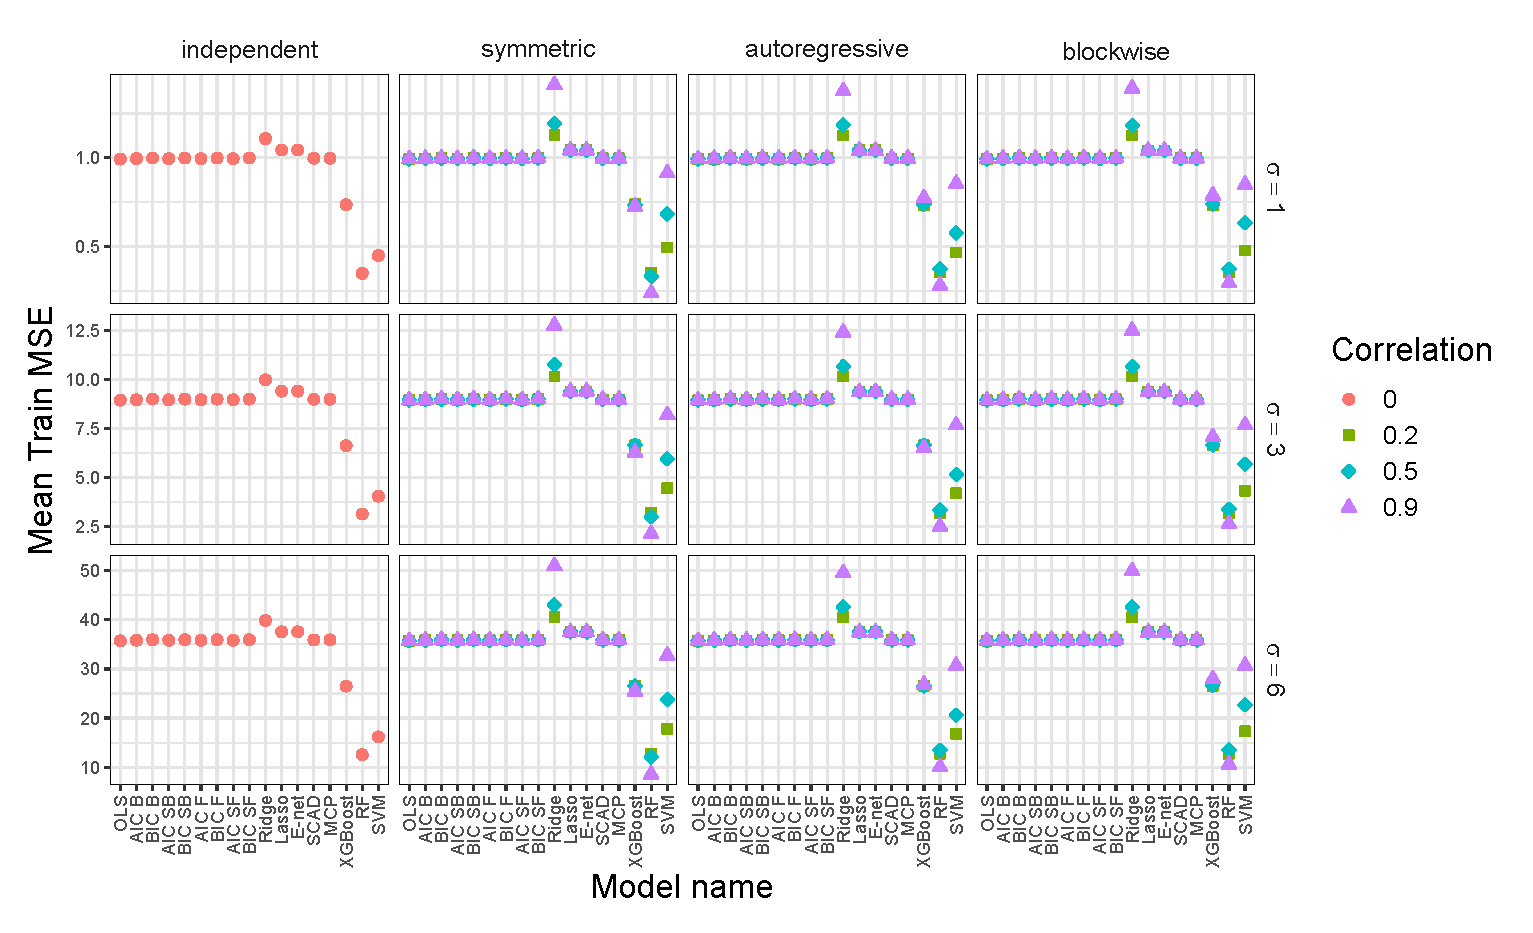
\includegraphics[width = \textwidth]{images/linear-facet/train-mse/facet_train_mse_1_1000_10.eps}
		\captionsetup{width = 0.8\textwidth}
		\caption{Average mean squared error using the training data for all linear simulations when $n = 1000$ and $p = 10$.}
		\label{fig:linear-train-mse-1000-10}
	\end{figure}
	
	\begin{figure}[h!]
		\centering
		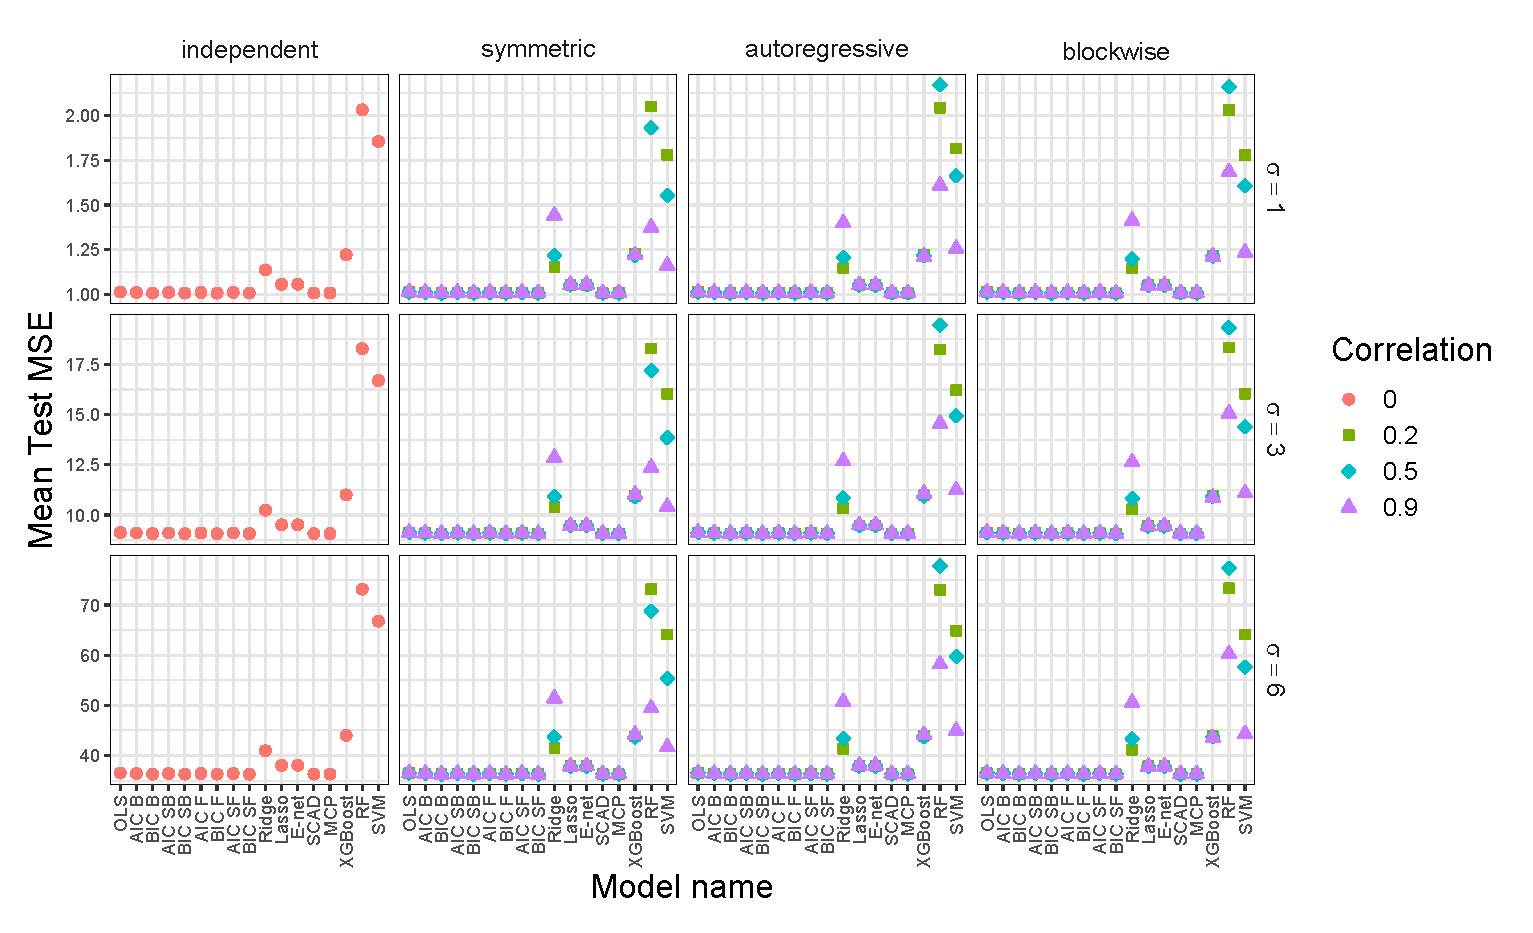
\includegraphics[width = \textwidth]{images/linear-facet/test-mse/facet_test_mse_1_1000_10.eps}
		\captionsetup{width = 0.8\textwidth}
		\caption{Average mean squared error using the test data for linear simulations when $n = 1000$ and $p = 10$.}
		\label{fig:linear-test-mse-1000-10}
	\end{figure}
	
	\begin{figure}[h!]
		\centering
		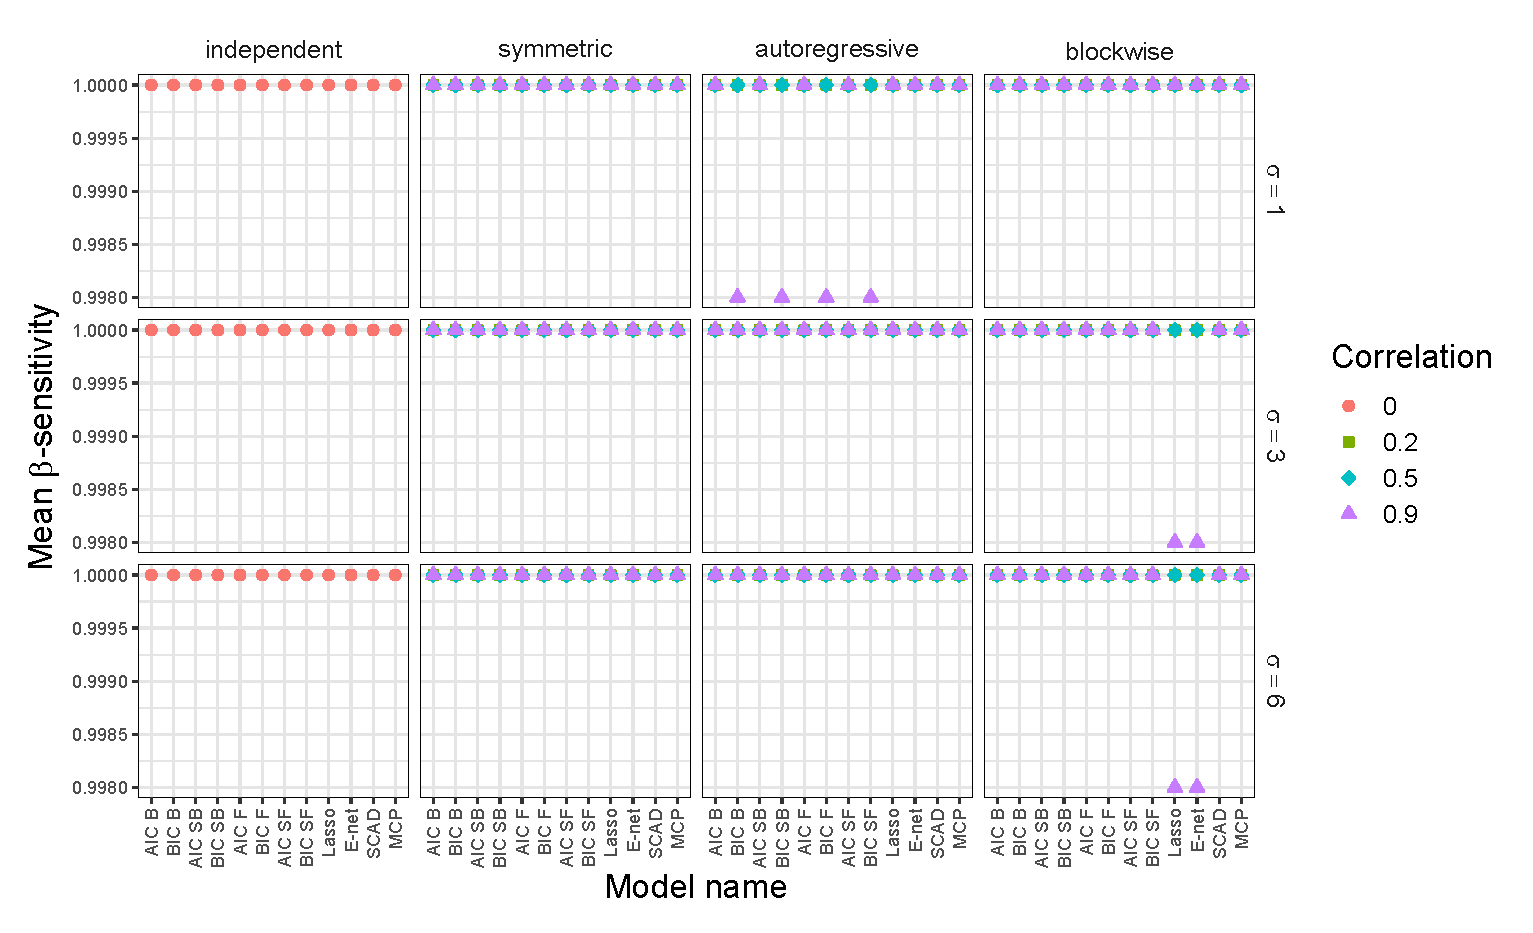
\includegraphics[width = \textwidth]{images/linear-facet/sensitivity/facet_sensitivity_1_1000_10.eps}
		\captionsetup{width = 0.8\textwidth}
		\caption{Average $\beta$-sensitivity for linear simulations when $n = 1000$ and $p = 10$.}
		\label{fig:linear-sensitivity-1000-10}
		
		\bigskip
		
		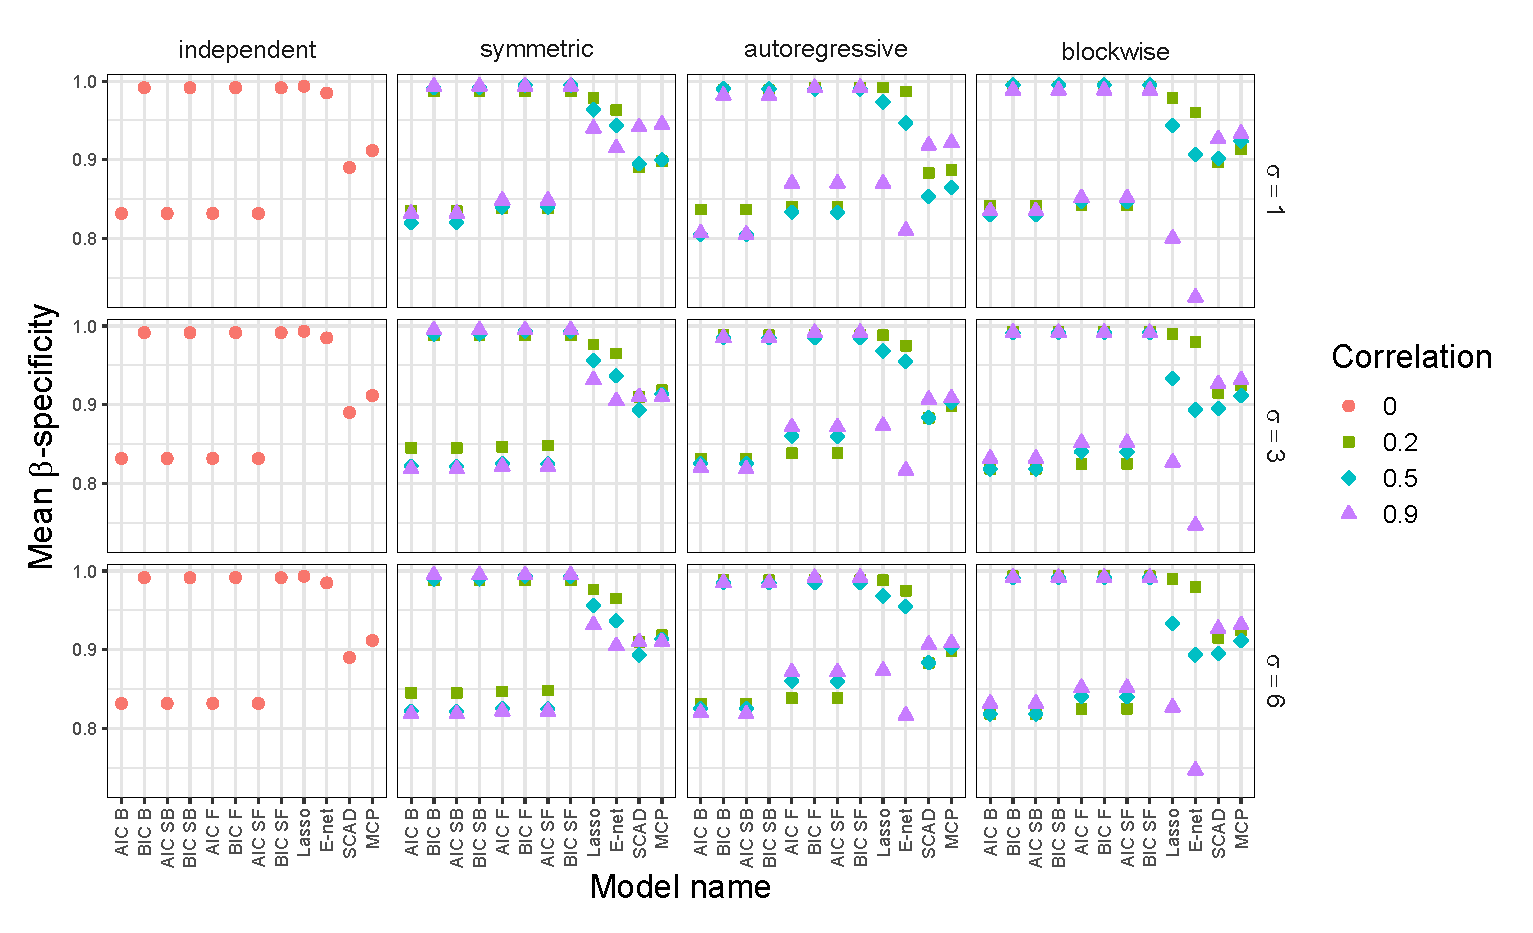
\includegraphics[width = \textwidth]{images/linear-facet/specificity/facet_specificity_1_1000_10.eps}
		\captionsetup{width = 0.8\textwidth}
		\caption{Average $\beta$-specificity for linear simulations when $n = 1000$ and $p = 10$.}
		\label{fig:linear-specificity-1000-10}
	\end{figure}
	
	We see that the linear models have very similar train and test mean squared errors. For these models, the mean squared error is approximately equal to $\sigma^2$, the square of the random error. We also see that for all of the linear models except for ridge regression, the type and strength of correlation has little effect on model performance. However, ridge regression performs worse when the correlation is high.
	
	The non-linear models all have lower training mean squared errors compared to the linear models. However, they also have higher test mean squared errors. We see that gradient boosting is not affected too strongly by the amount of correlation; on the other hand, we see that random forest and support vector machine models have better test performance when there is a strong correlation between predictors.
	
	Figure \ref{fig:linear-sensitivity-1000-10} displays the average $\beta$-sensitivity for each model that performs variable selection when $n = 1000$ and $p = 10$. See Table \ref{tab:linear-sensitivity-1000-10} for a table of these results. We see that almost all the models were able to correctly identify all of the non-zero coefficients when $n = 1000$ and $p = 10$. The only exceptions were lasso and elastic-net models when the correlation structure was blockwise and the strength of the correlation was 0.9.
	
	Figure \ref{fig:linear-specificity-1000-10} shows the average $\beta$-specificity for each model. Exact numerical values are given in Table \ref{tab:linear-specificity-1000-10}. We see that the subset selection models that used BIC made almost zero mistakes when identifying predictors as zero. In contrast, wrapper models fitted using AIC made more mistakes. We see that lasso and elastic-net made almost no mistakes when the correlation was low; in fact, when the correlation structure was independent, lasso made the fewest incorrect estimates out of all the models. As the correlation increases, lasso and elastic-net made more incorrect predictions. SCAD and MCP made more incorrect predictions than lasso and elastic-net in general. However, SCAD and MCP were also somewhat more resilient to an increase in correlation.
	
	\end{comment}
	
	Figure \ref{fig:linear-train-mse} shows the average MSE for the simulated models on training data; Figure \ref{fig:linear-test-mse} shows the same results but for test data. Figure \ref{fig:linear-sensitivity} and \ref{fig:linear-specificity} display the $\beta$-sensitivity and $\beta$-specificity for the linear models that perform variable selection.
	
	\begin{figure}[t!]
		\centering
		\begin{minipage}[t]{0.47\textwidth}
			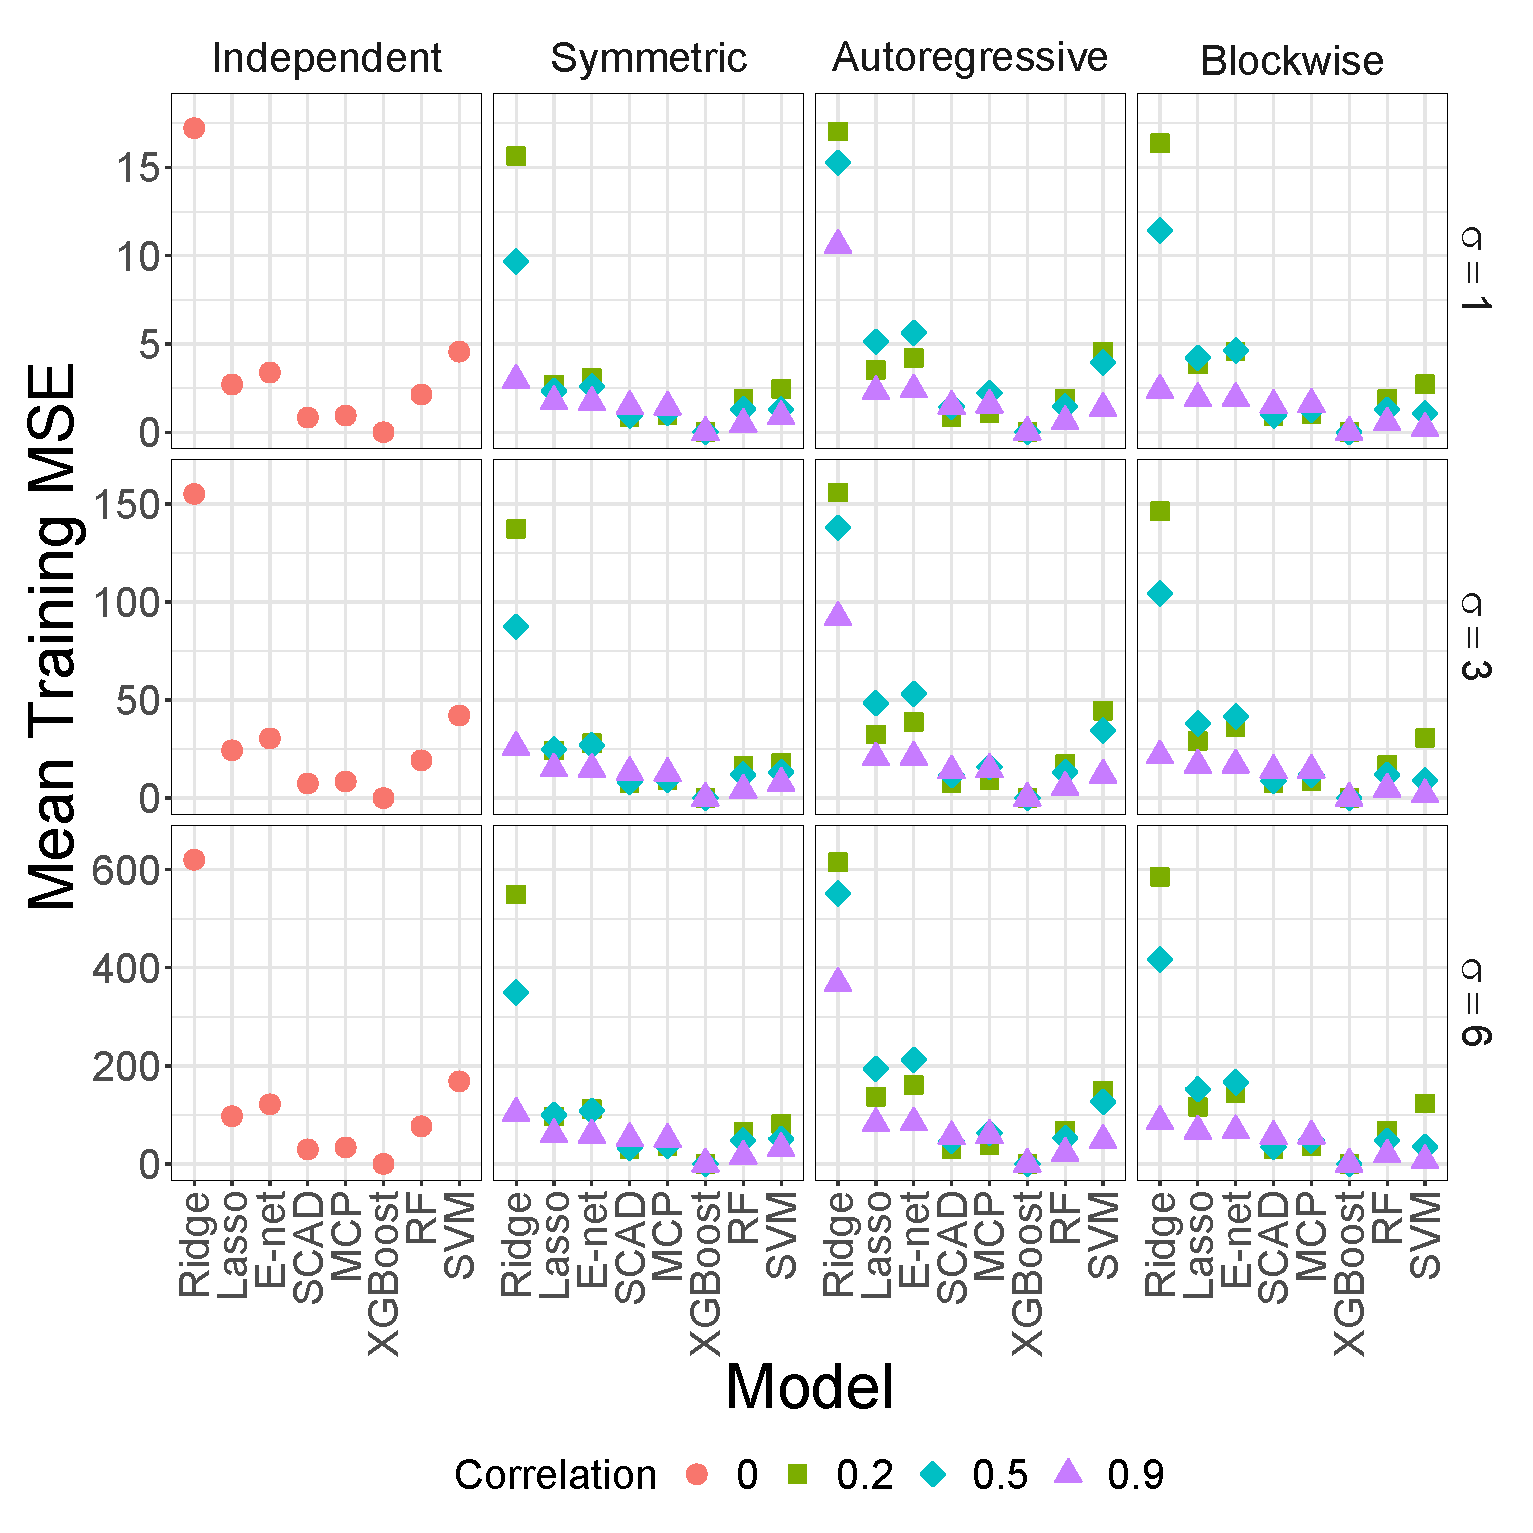
\includegraphics[width = \textwidth]{images/facet/publication_facet_train_mse_linear_50_2000.eps}
			\captionsetup{width = 0.95\textwidth}
			\caption{Average mean square error using training data for linear simulations when $n = 50$ and $p = 	2000$.}
			\label{fig:linear-train-mse}
		\end{minipage}
		\hspace{6pt}
		\begin{minipage}[t]{0.47\textwidth}
			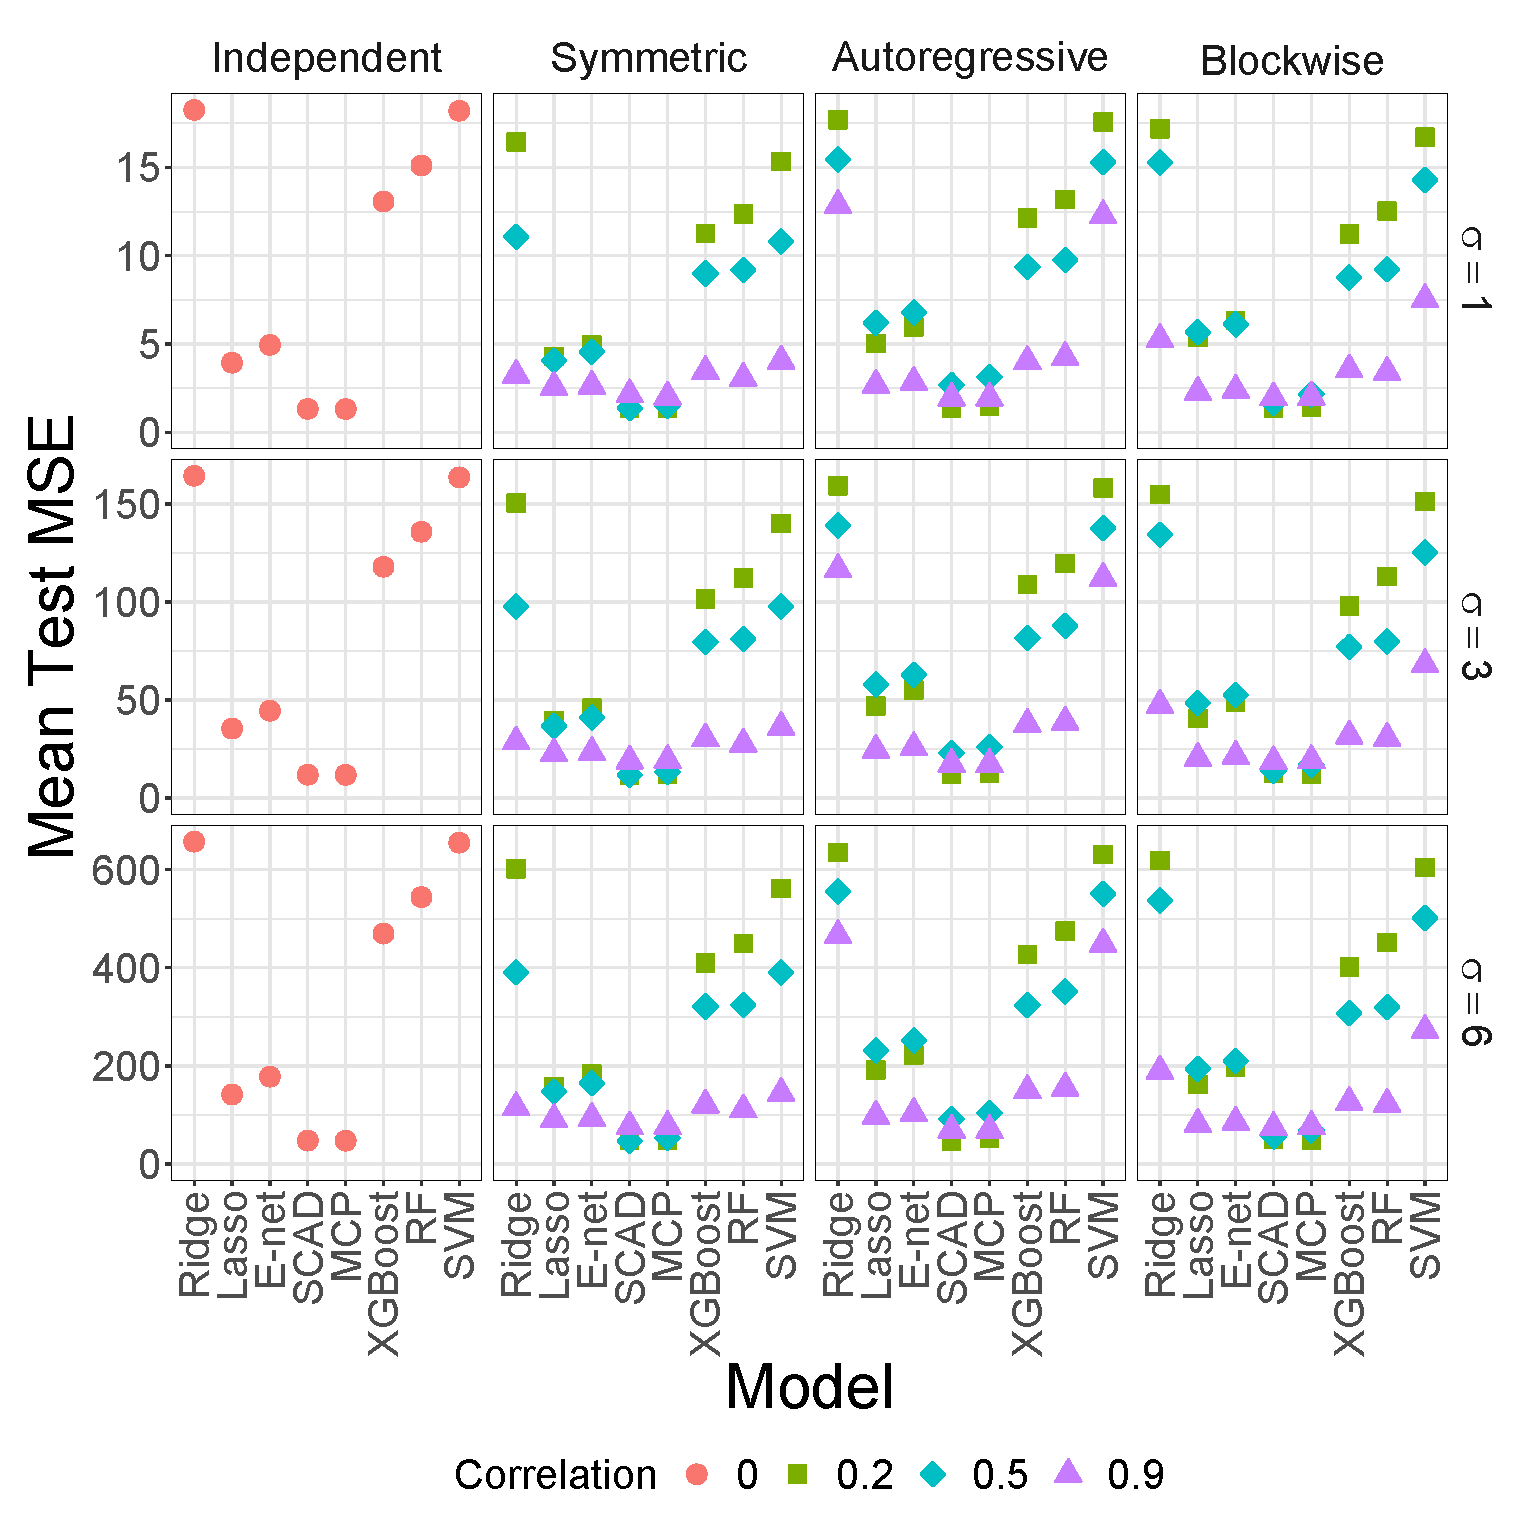
\includegraphics[width = \textwidth]{images/facet/publication_facet_test_mse_linear_50_2000.eps}
			\captionsetup{width = 0.95\textwidth}
			\caption{Average mean square error using testing data for linear simulations when $n = 50$ and $p = 	2000$.}
			\label{fig:linear-test-mse}
		\end{minipage}
		\vspace{6pt}
		
		\begin{minipage}[t]{0.47\textwidth}
			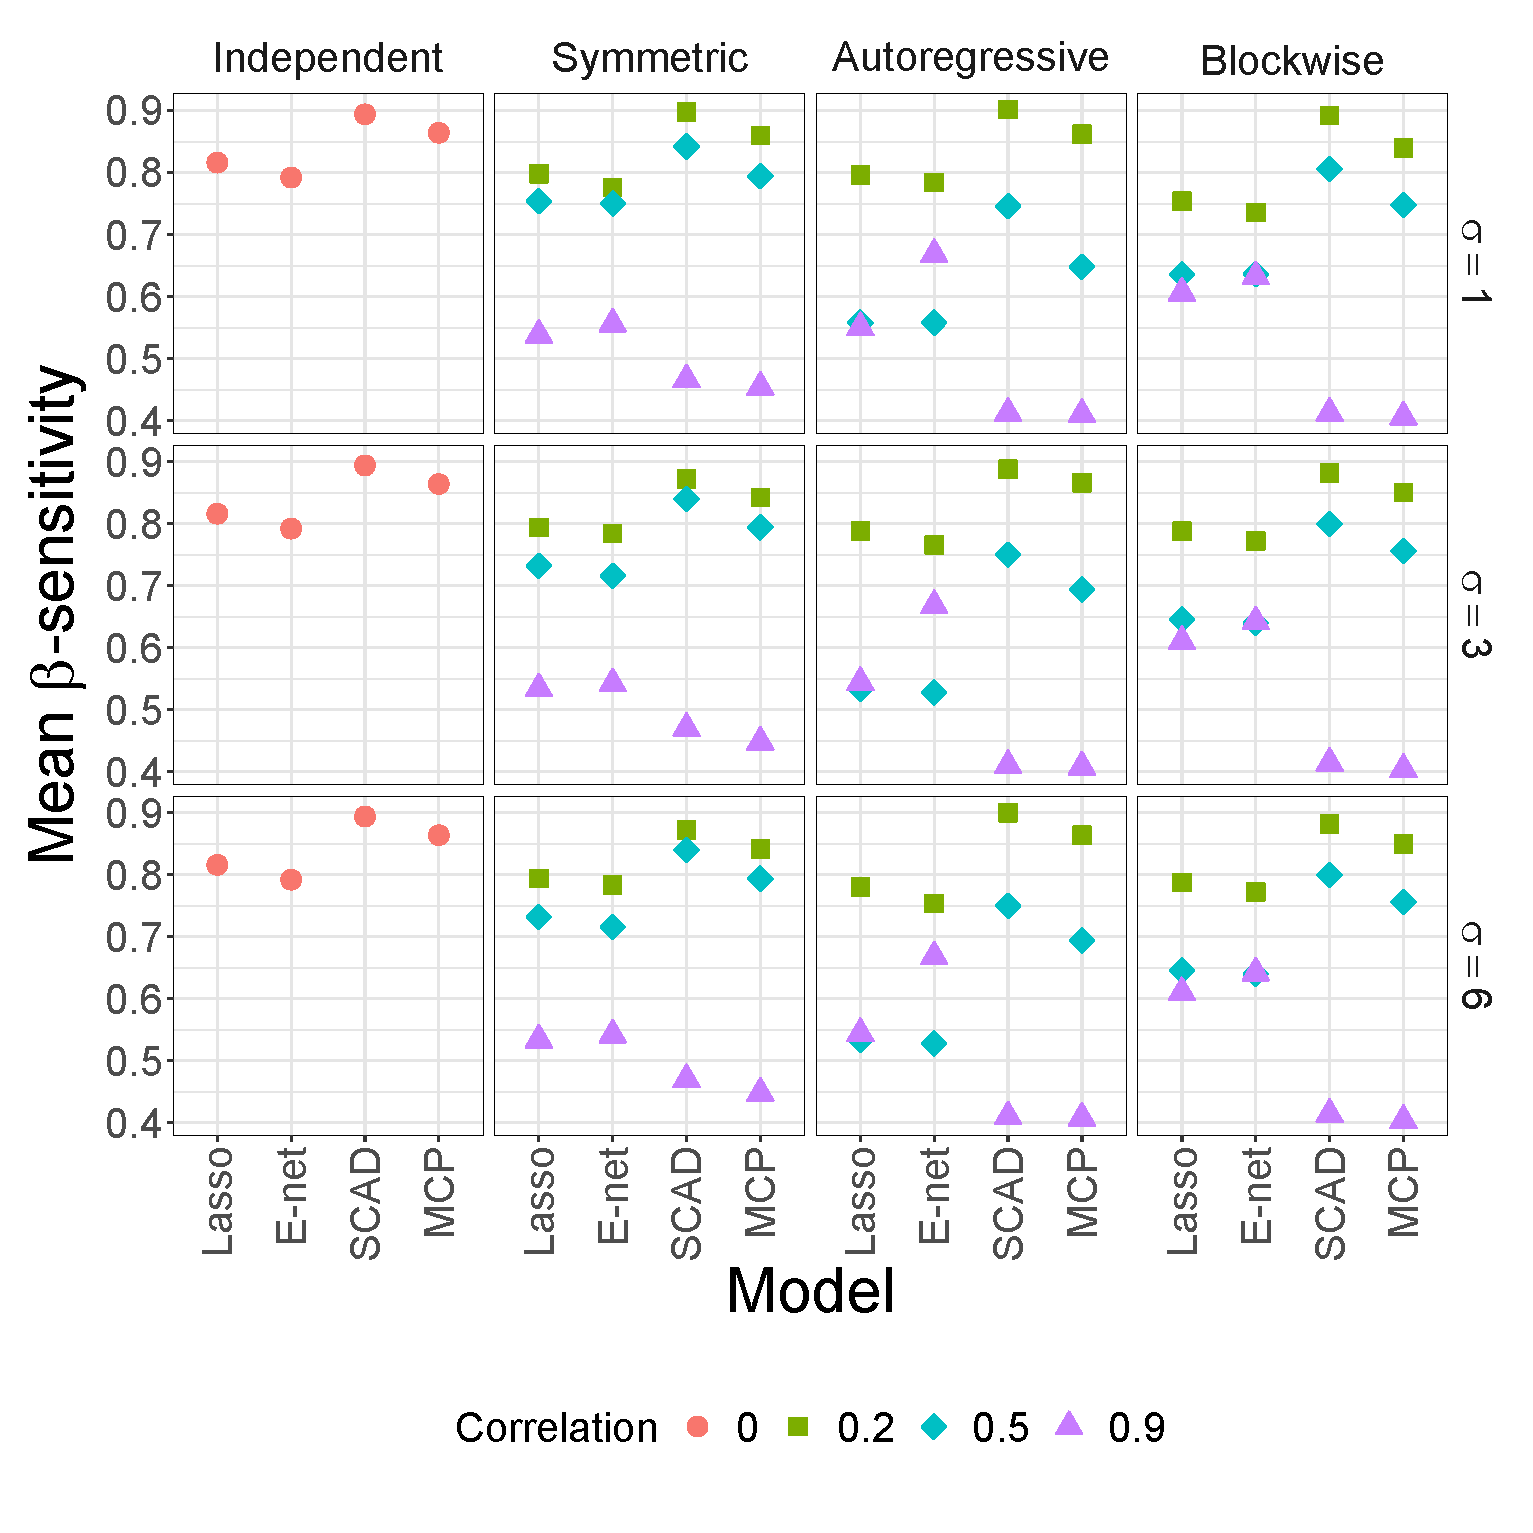
\includegraphics[width = \textwidth]{images/facet/publication_facet_sensitivity_linear_50_2000.eps}
			\captionsetup{width = 0.95\textwidth}
			\caption{Average $\beta$-sensitivity for linear simulations when $n = 50$ and $p = 	2000$.}
			\label{fig:linear-sensitivity}
		\end{minipage}
		\hspace{6pt}
		\begin{minipage}[t]{0.47\textwidth}
			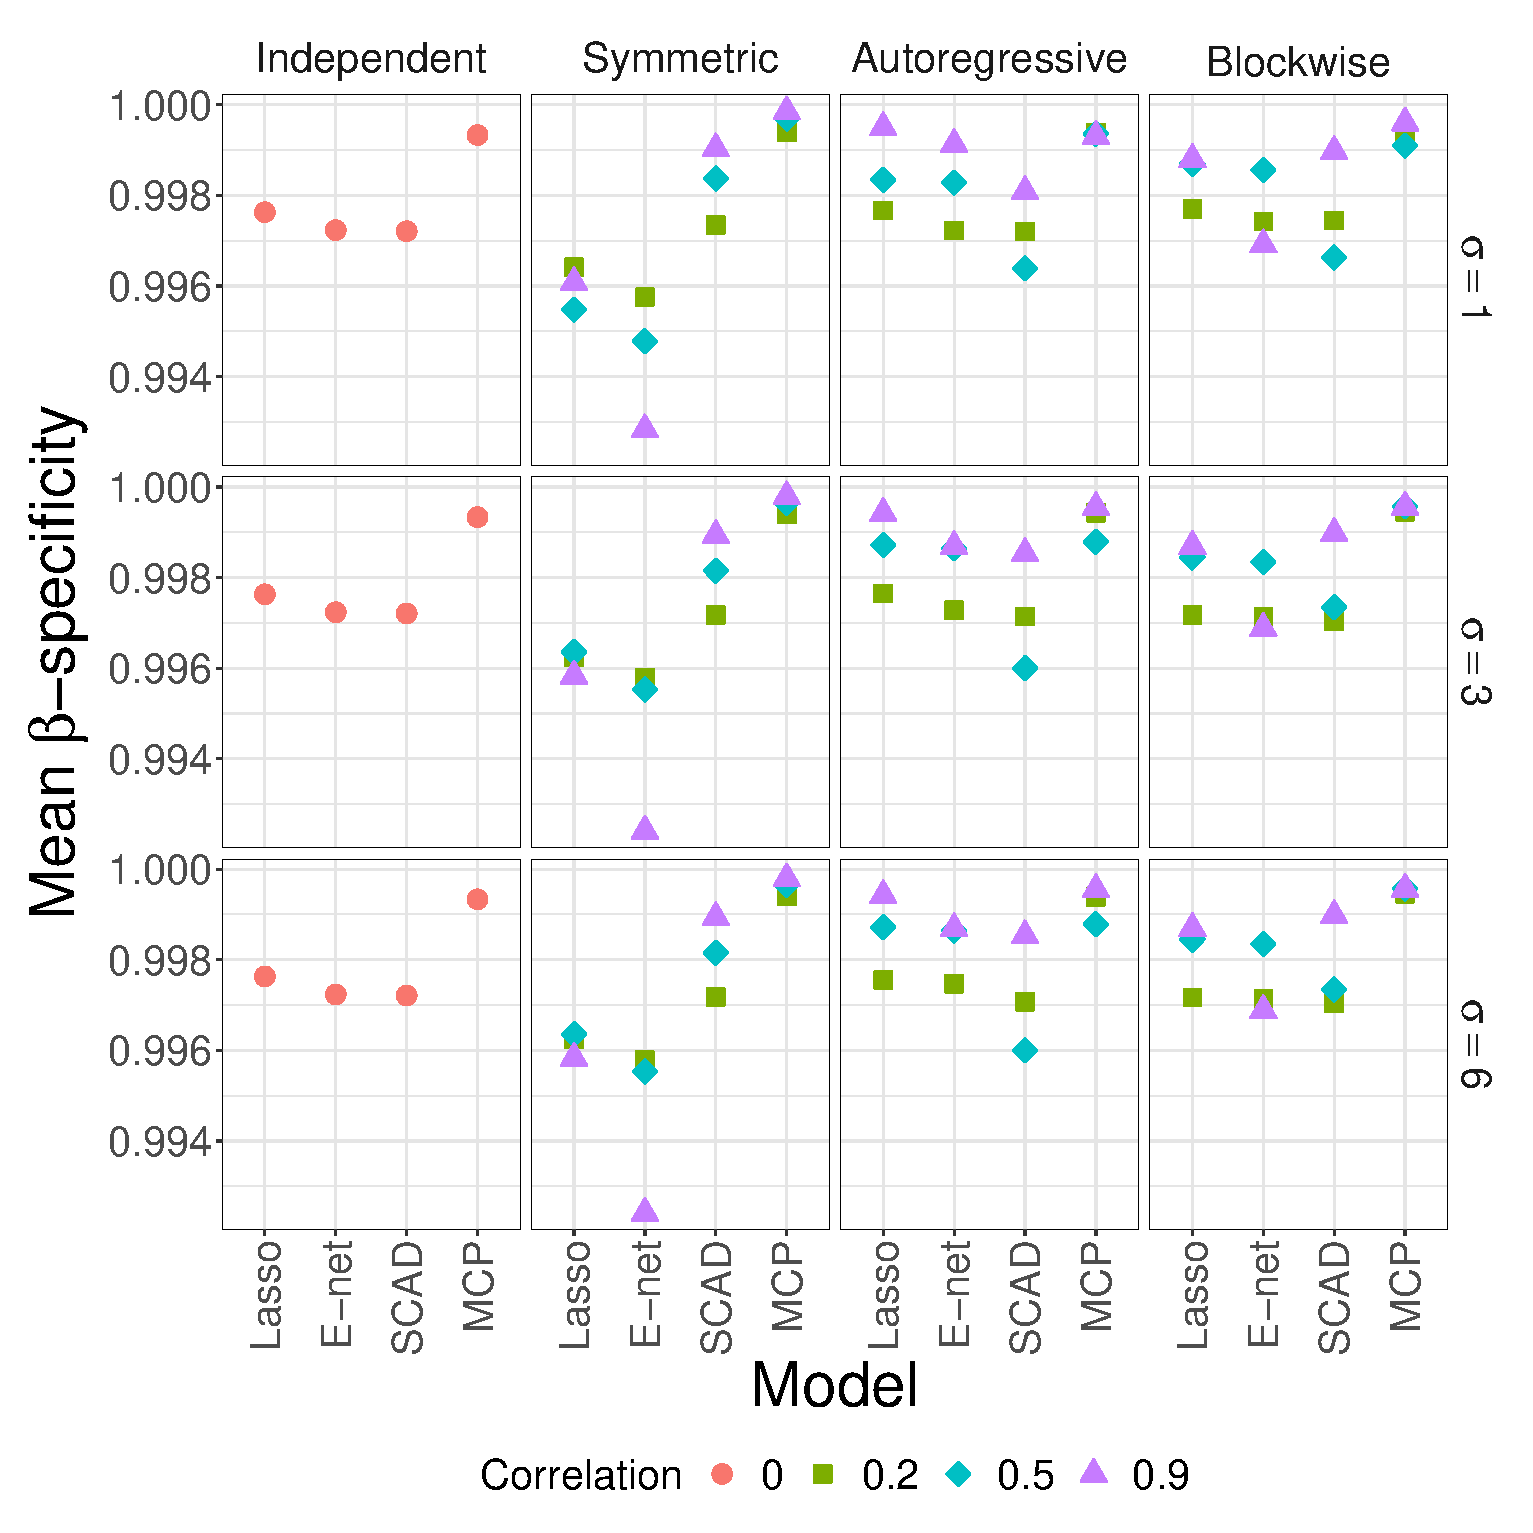
\includegraphics[width = \textwidth]{images/facet/publication_facet_specificity_linear_50_2000.eps}
			\captionsetup{width = 0.95\textwidth}
			\caption{Average $\beta$-specificity for linear simulations when $n = 50$ and $p = 	2000$.}
			\label{fig:linear-specificity}
		\end{minipage}
	\end{figure}

	We see that the mean squared error for lasso and elastic-net are generally larger than SCAD and MCP for both the training data and test data. Gradient boosting has almost zero training mean squared error under all conditions, but has a relatively large test error. Random forest and support vector machine models have a moderate training error but a large test error. Interestingly, we see that the non-linear models all perform better when there is a strong correlation between predictors. On the other hand, the linear models are somewhat less affected by the correlation.
	
	Looking at Figure \ref{fig:linear-sensitivity}, we see that all of the models predict most of the non-zero coefficients when the correlation is low. When the correlation is high, all of the models struggle to identify the correct predictors. SCAD and MCP perform the best when the correlation is low but perform the worst when the correlation is high. Elastic-net performs particularly well compared to the other models when the correlation is high, especially when the correlation structure is autoregressive.
	
	Now, consider the results for $\beta$-specificity from Figure \ref{fig:linear-specificity}. MCP appears to make the fewest mistakes when choosing zero coefficients. The performance of the other models depends heavily on the type of correlation and the correlation strength. Lasso and elastic-net perform the worst when the correlation structure is symmetric compound, whereas SCAD performs poorly when the correlation structure is autoregressive or blockwise. We also see that the models correctly identify more coefficients as being zero as the correlation increases.
	
	\subsection{Non-linear Simulation Results}
	Now, we will highlight some results from the simulations for Model 2 given by Equation \ref{eqn:nonlinear-response}.
	
	\begin{comment}
	
	First, we will consider the extreme where $n = 1000$ and $p = 10$. Figures \ref{fig:nonlinear-train-mse-1000-10} and \ref{fig:nonlinear-test-mse-1000-10} show the average train MSE and test MSE, respectively. We see that all of the linear models have a high mean squared error on both training and test data. Ridge, lasso, and elastic-net had slightly higher mean squared errors than the other linear models. The correlation structure and correlation strength appear to have little effect on the performance of the linear models. Although increasing $\sigma$ (the standard deviation of the random error) significantly increases the mean squared errors, it seems to affect all of the models equally.
	
	On the other hand, the machine learning models have low mean squared errors on both training and test data. Gradient boosting has the best performance out of these three models, while support vector machines perform the worst. However, all three models greatly outperform any of the linear models. We also note that XGBoost and random forest models seem unaffected by the correlation strength, correlation value, and random error. Support vector machines appear to perform worse relative to the other machine learning models when $\sigma$ is small.
	\begin{figure}[h!]
		\centering
		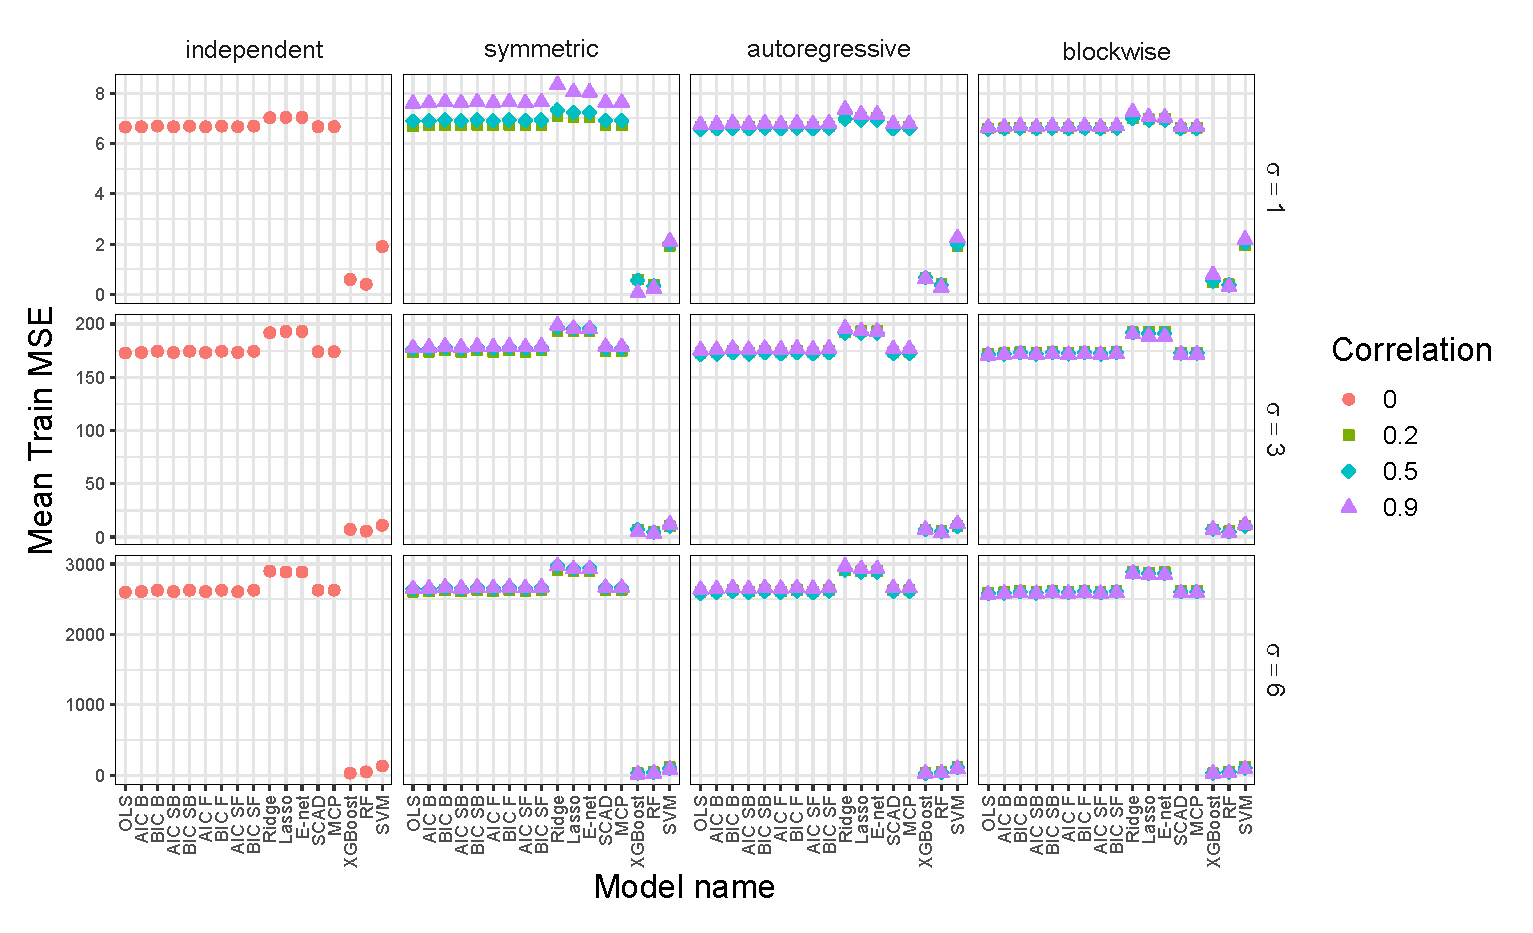
\includegraphics[width = \textwidth]{images/nonlinear-facet/train-mse/facet_train_mse_2_1000_10.eps}
		\captionsetup{width = 0.8\textwidth}
		\caption{Average mean square error using training data for non-linear simulations when $n = 1000$ and $p = 10$.}
		\label{fig:nonlinear-train-mse-1000-10}
	\end{figure}
	
	\begin{figure}[h!]
		\centering
		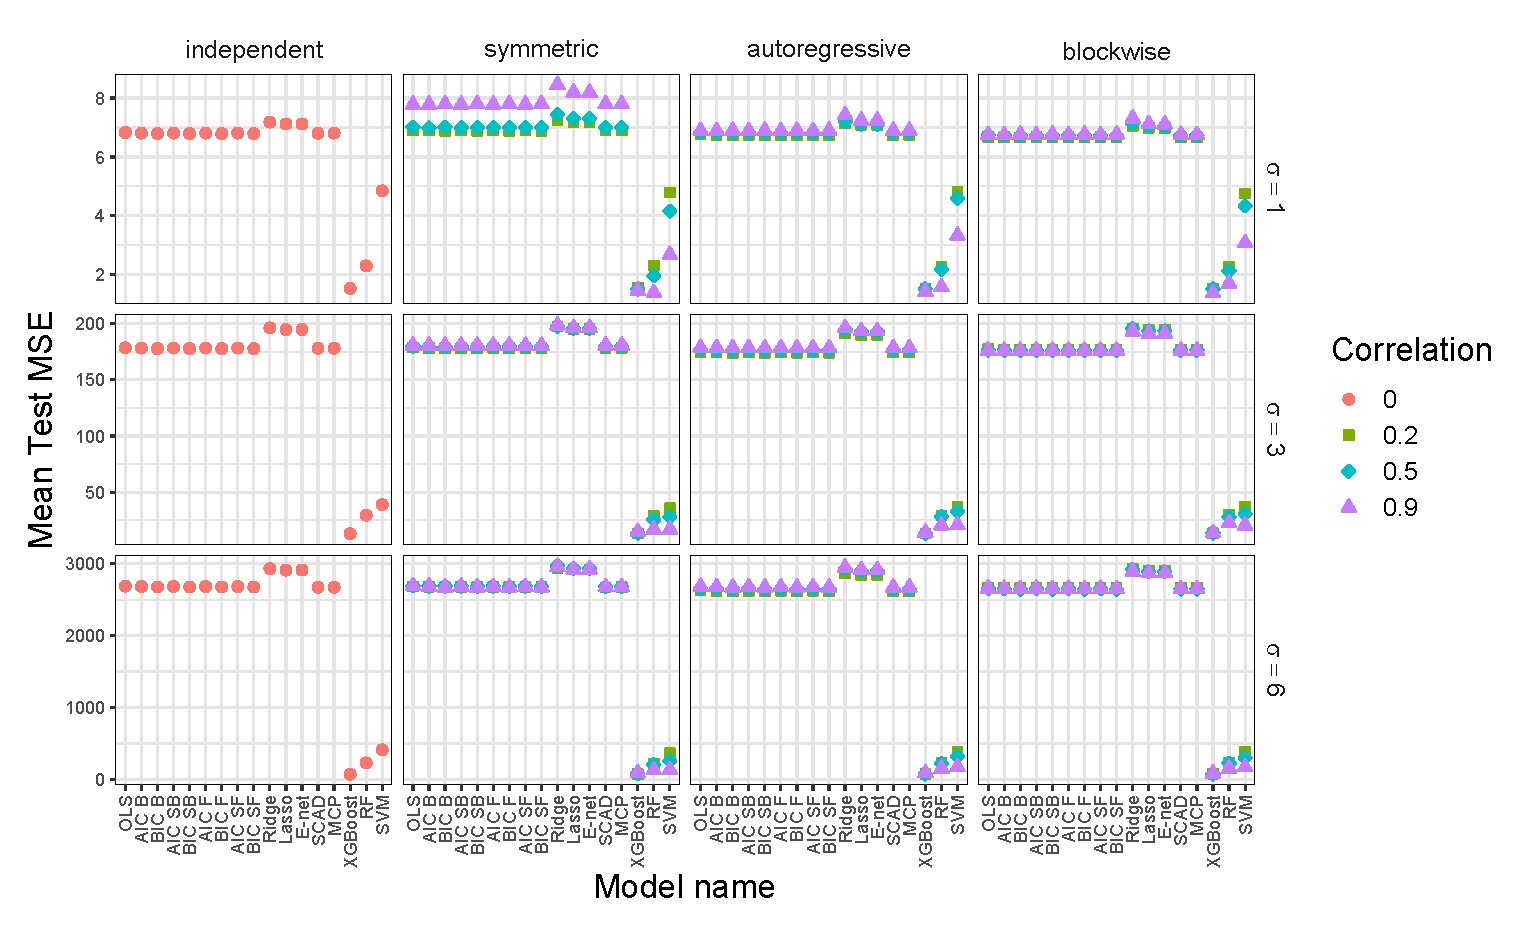
\includegraphics[width = \textwidth]{images/nonlinear-facet/test-mse/facet_test_mse_2_1000_10.eps}
		\captionsetup{width = 0.8\textwidth}
		\caption{Average mean square error using test data for non-linear simulations when $n = 1000$ and $p = 10$.}
		\label{fig:nonlinear-test-mse-1000-10}
	\end{figure}
	
	Figures \ref{fig:nonlinear-sensitivity-1000-10} and \ref{fig:nonlinear-specificity-1000-10} show the average $\beta$-sensitivity and $\beta$-specificity for every model from the non-linear simulations when $n = 1000$ and $p  =10$. We see that lasso and elastic-net are the most picky models, having the lowest $\beta$-sensitivity and highest $\beta$-specificity. This means that lasso and elastic-net estimated more of the coefficients as zero compared to the other models. Another observation is that for lasso and elastic-net, an increase in the correlation led to more coefficients being estimated as non-zero (since the $\beta$-sensitivity increases and the $\beta$-specificity decreases). All of the other models exhibit the opposite behavior, estimating more predictors as having coefficients equal to zero as the correlation increases.
	\begin{figure}[h!]
		\centering
		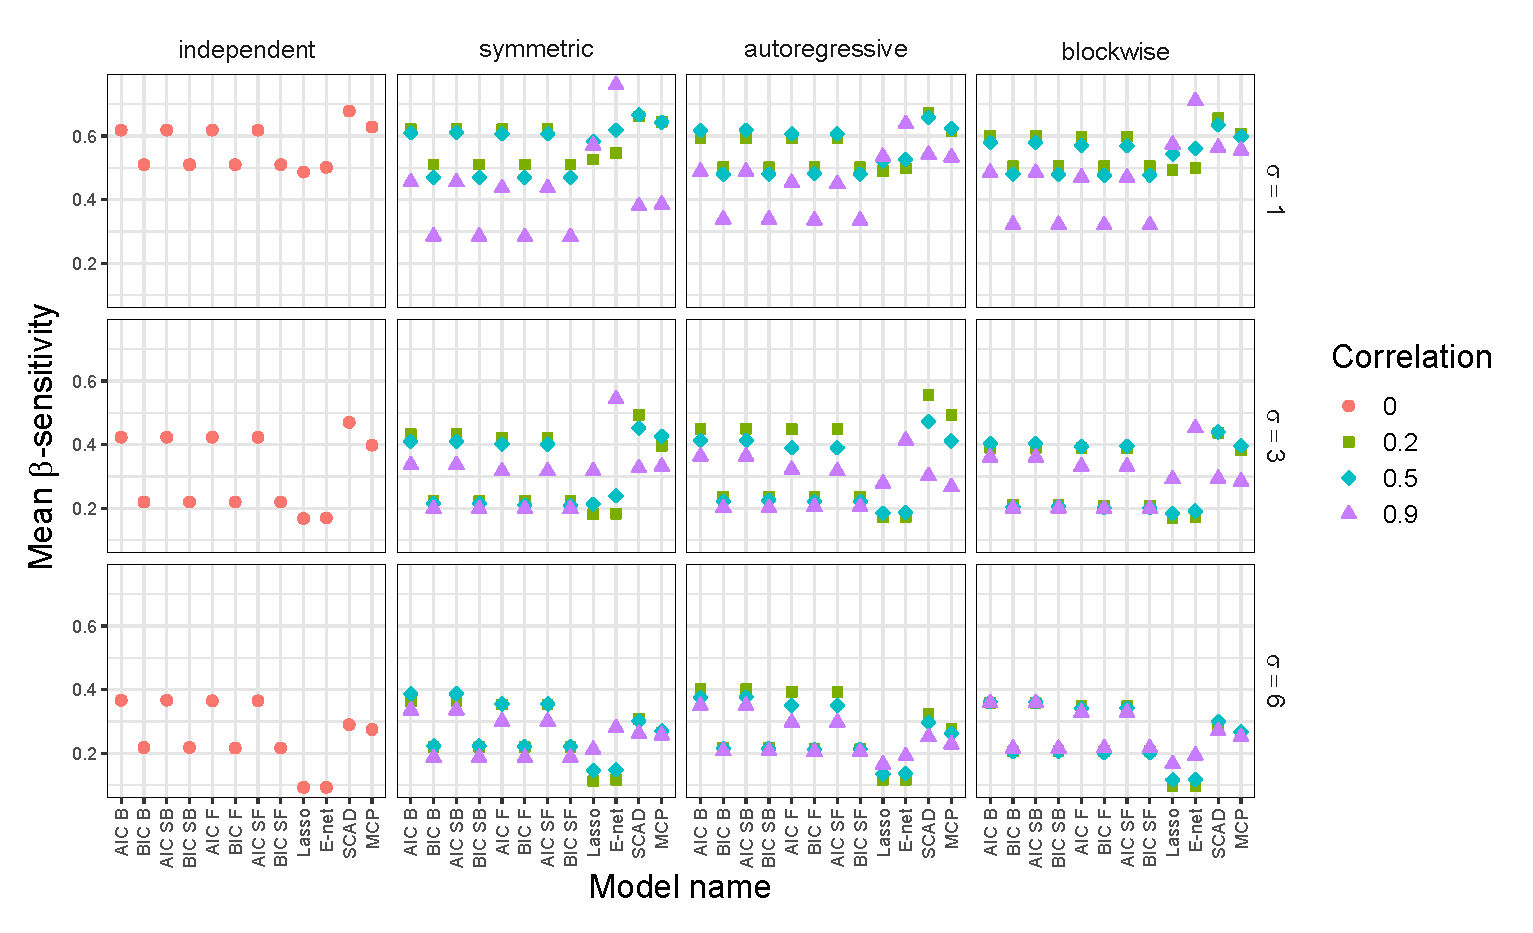
\includegraphics[width = \textwidth]{images/nonlinear-facet/sensitivity/facet_sensitivity_2_1000_10.eps}
		\captionsetup{width = 0.8\textwidth}
		\caption{Average $\beta$-sensitivity for non-linear simulations when $n = 1000$ and $p = 10$.}
		\label{fig:nonlinear-sensitivity-1000-10}
	\end{figure}
	
	\begin{figure}[h!]
		\centering
		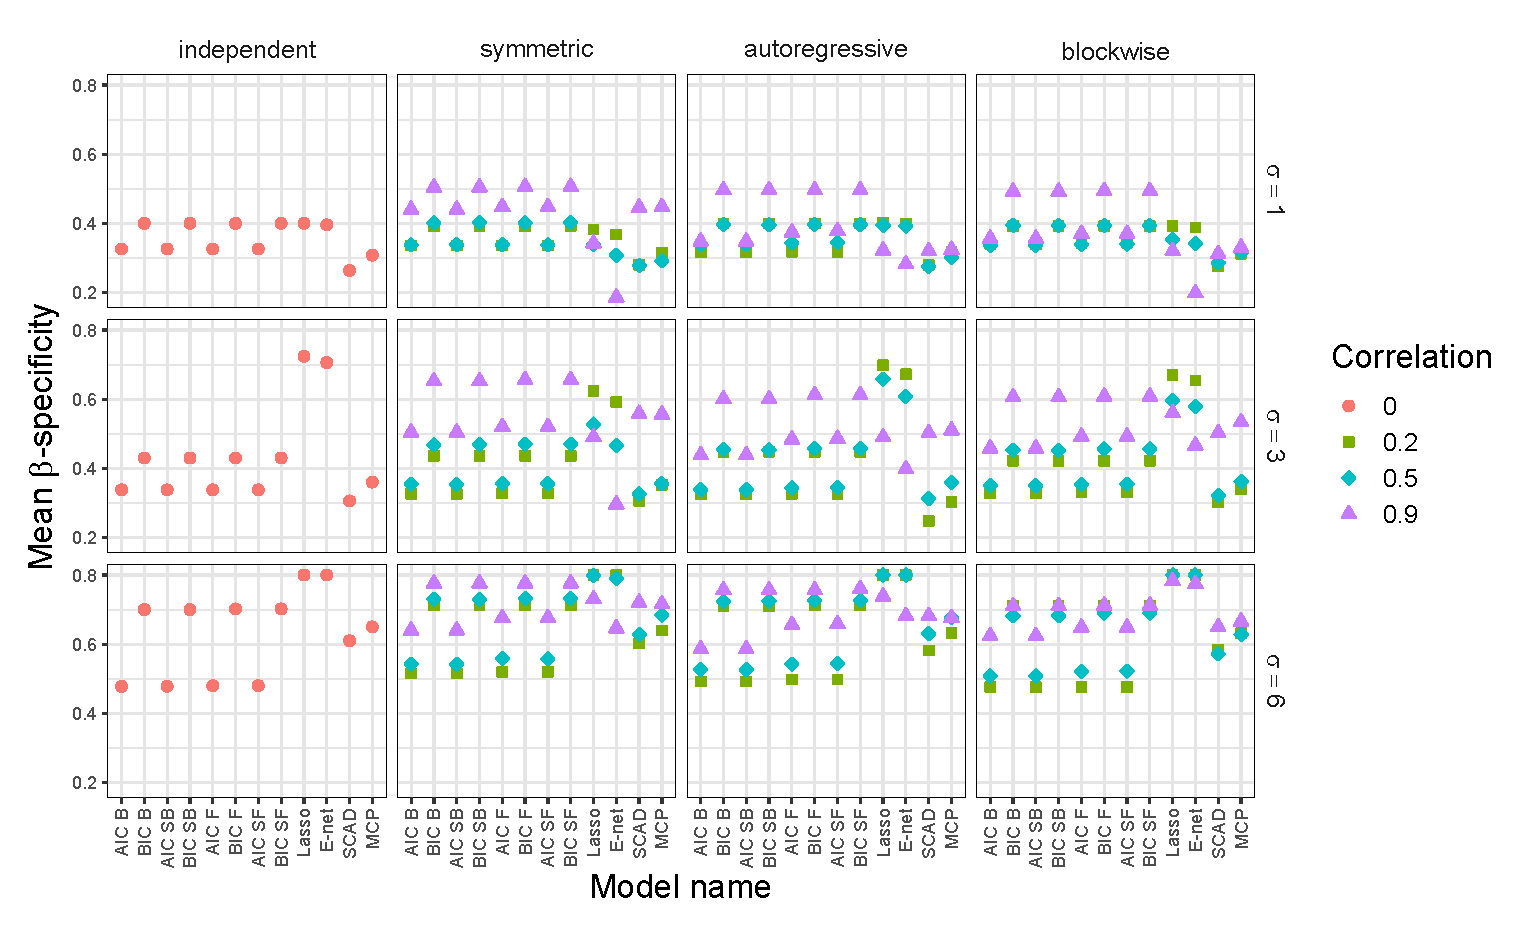
\includegraphics[width = \textwidth]{images/nonlinear-facet/specificity/facet_specificity_2_1000_10.eps}
		\captionsetup{width = 0.8\textwidth}
		\caption{Average $\beta$-specificity for non-linear simulations when $n = 1000$ and $p = 10$.}
		\label{fig:nonlinear-specificity-1000-10}
	\end{figure}
	
	\end{comment}
	
	Figures \ref{fig:nonlinear-train-mse} and \ref{fig:nonlinear-test-mse} show the average mean square errors on the training data and test data, respectively. We see that the linear and non-linear models have similar test mean squared errors. Another interesting observation is that the non-linear models all have a noticeably lower test mean squared error when the correlation between predictors is high. The linear models still perform significantly worse on the training data compared to the test data. 
	\begin{figure}[t!]
		\centering
		\begin{minipage}[t]{0.47\textwidth}
			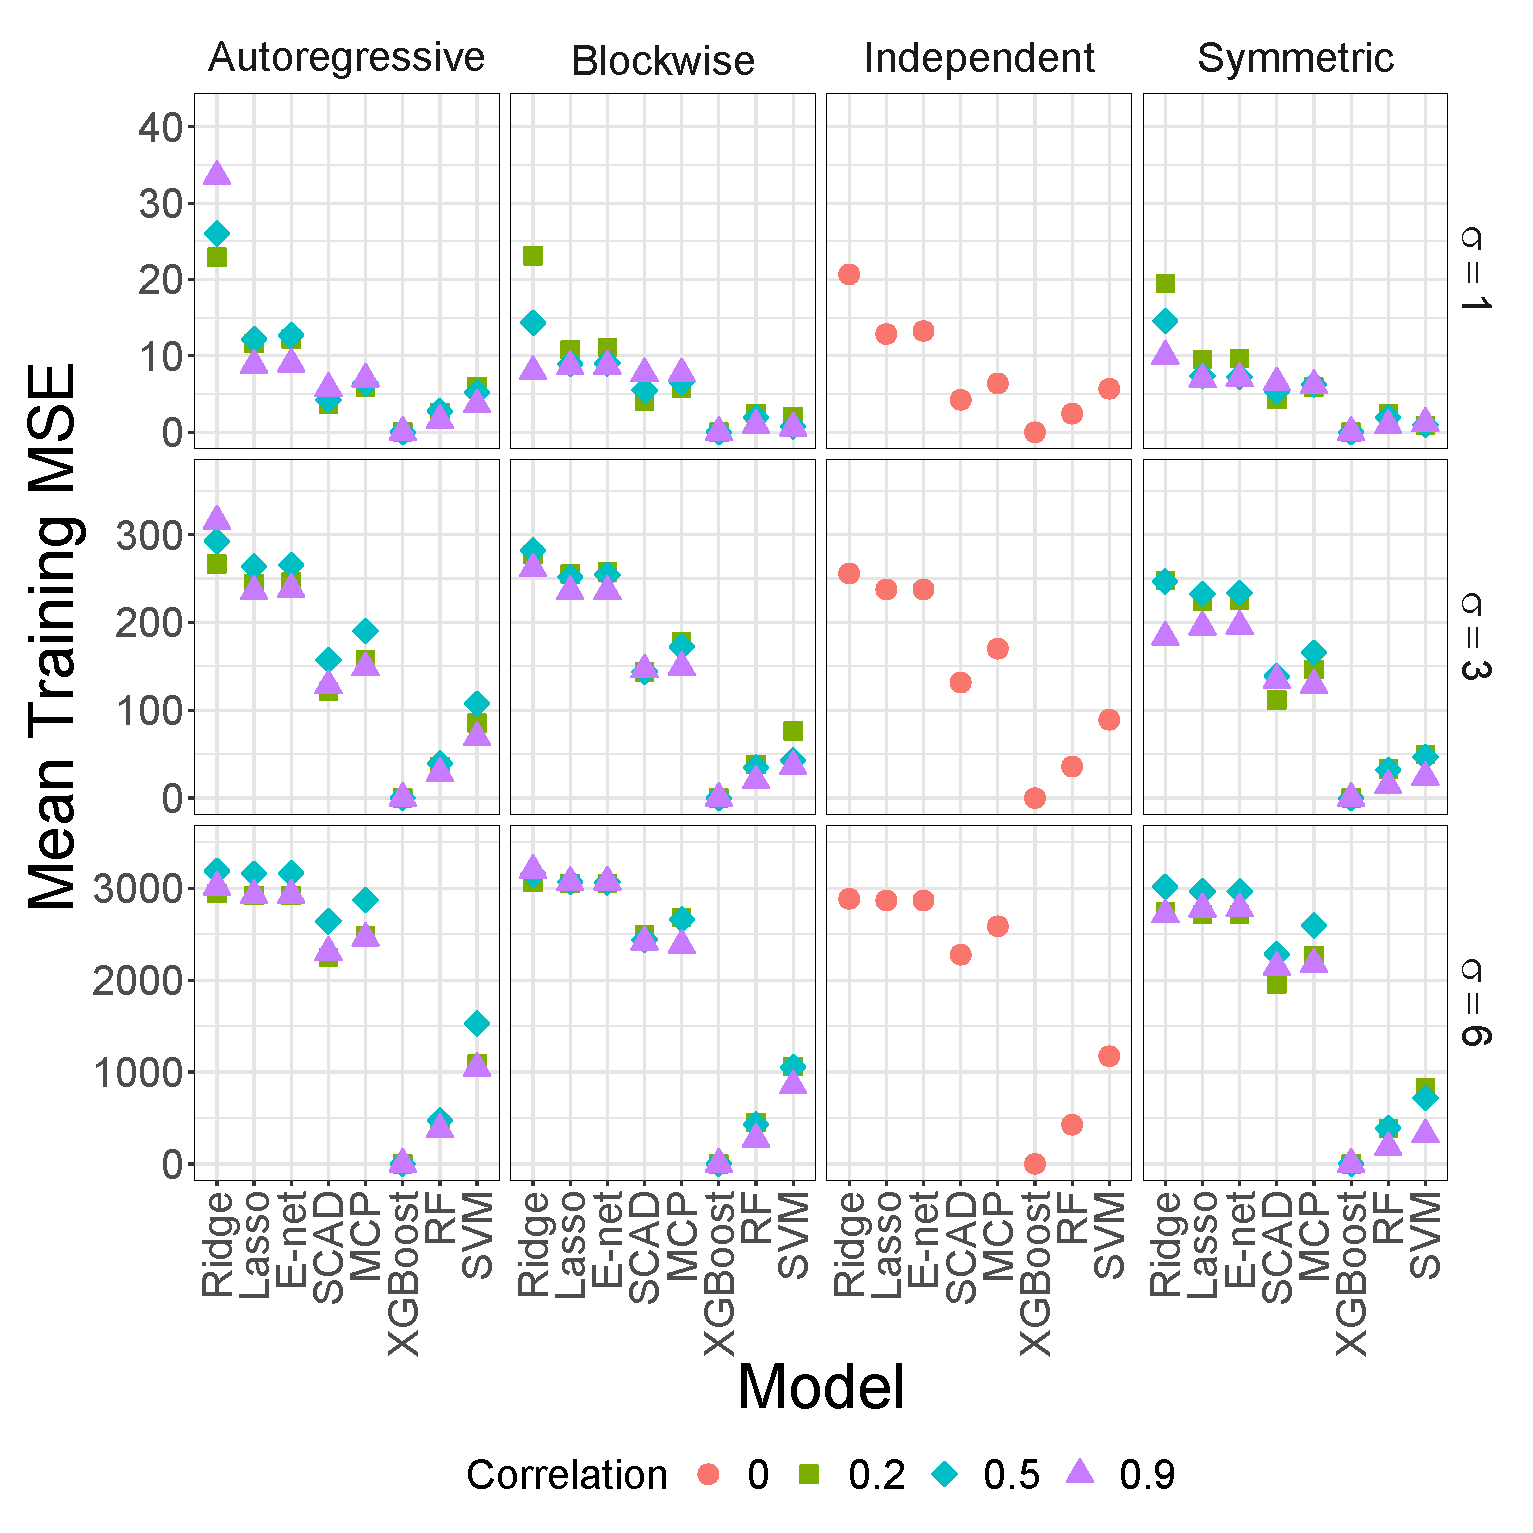
\includegraphics[width=\textwidth]{images/facet/publication_facet_train_mse_nonlinear_50_2000.eps}
			\captionsetup{width = 0.95\textwidth}
			\caption{Average mean square error using training data for non-linear simulations when $n = 50$ and $p = 	2000$.}
			\label{fig:nonlinear-train-mse}
		\end{minipage}
		\hspace{6pt}
		\begin{minipage}[t]{0.47\textwidth}
			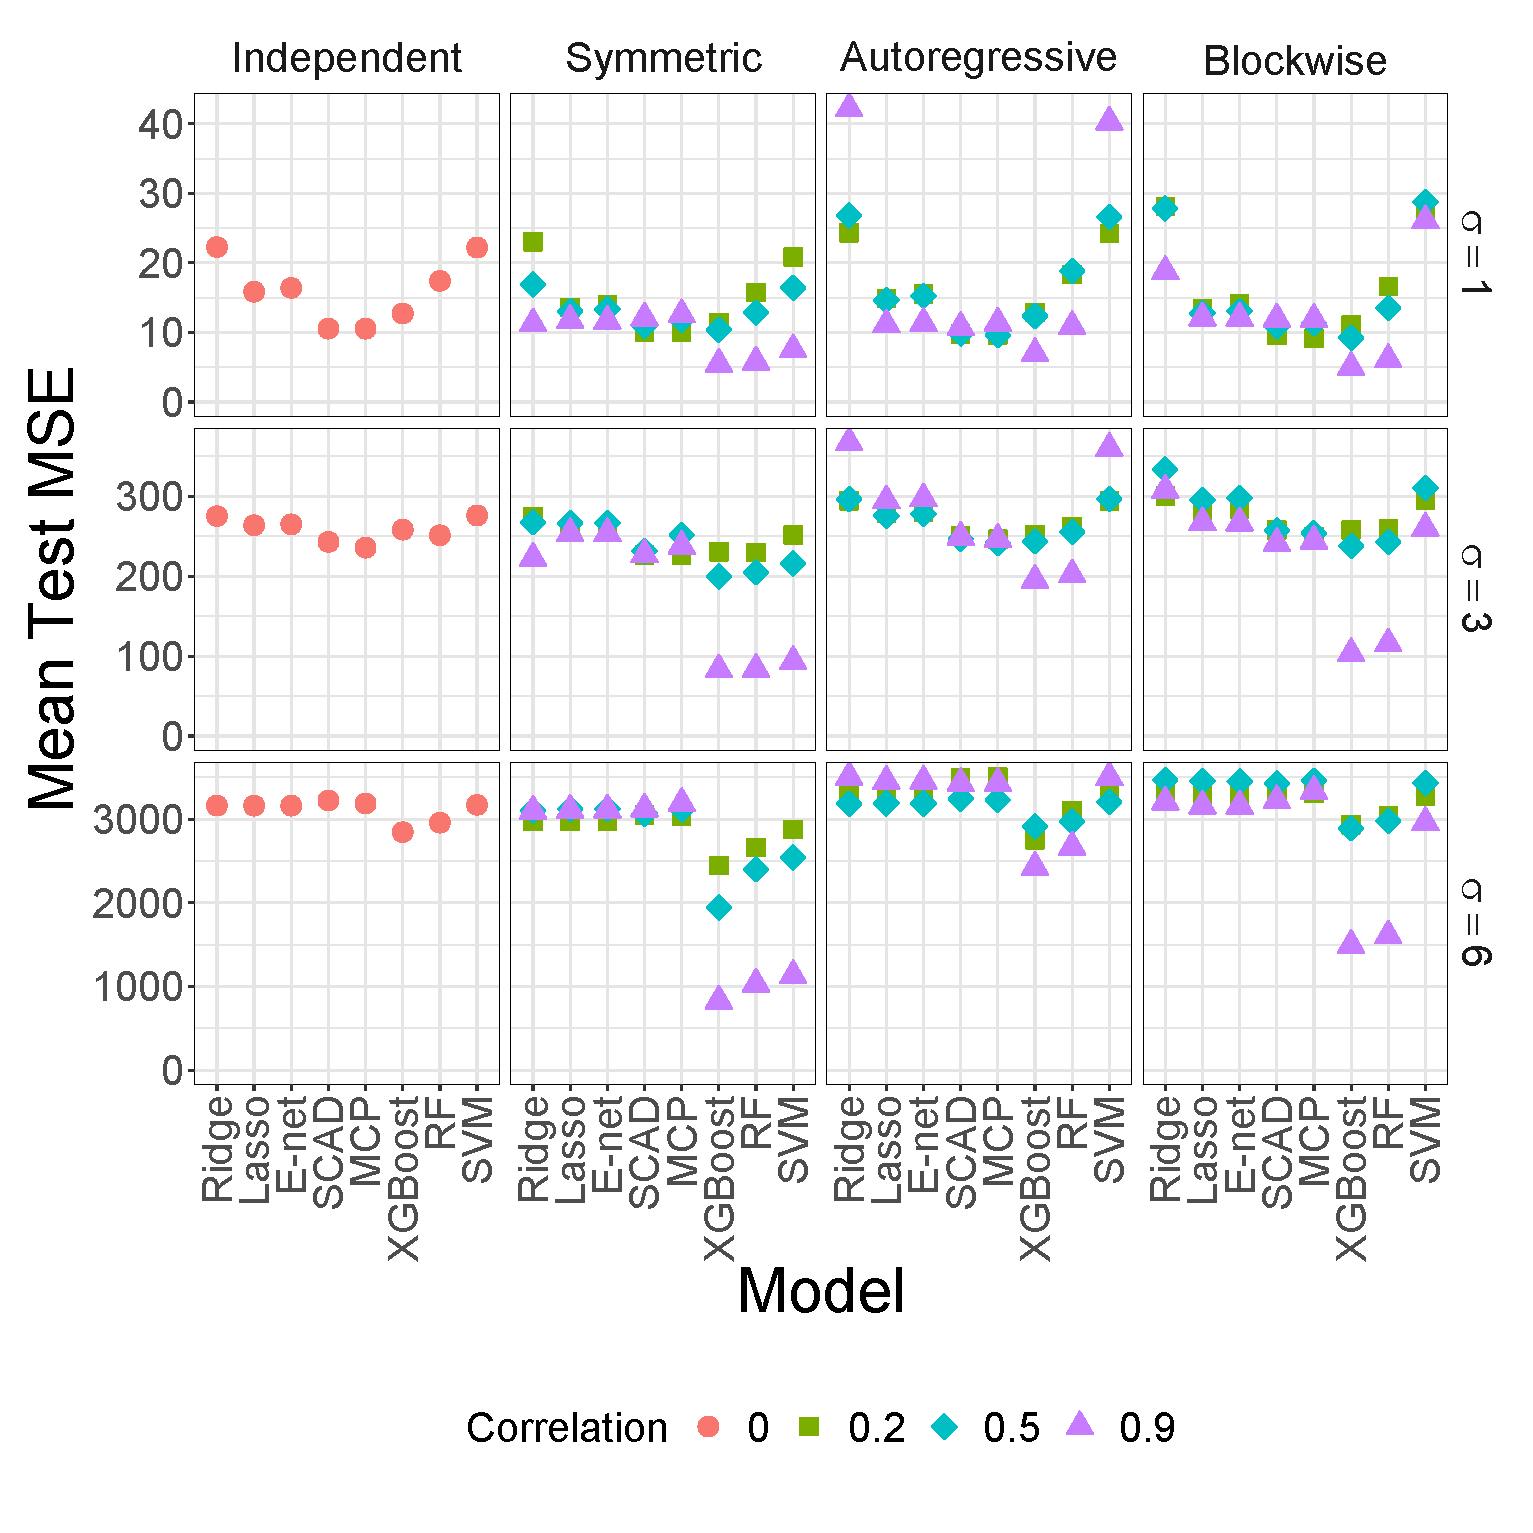
\includegraphics[width=\textwidth]{images/facet/publication_facet_test_mse_nonlinear_50_2000.eps}
			\captionsetup{width = 0.95\textwidth}
			\caption{Average mean square error using testing data for non-linear simulations when $n = 50$ and $p = 	2000$.}
			\label{fig:nonlinear-test-mse}
		\end{minipage}
	\end{figure}
	
	Figures \ref{fig:nonlinear-sensitivity} and \ref{fig:nonlinear-specificity} show the results for the $\beta$-sensitivity and $\beta$-specificity for the non-linear models. We see that all of the linear models estimate almost all of the coefficients as being equal to zero! SCAD and MCP were slightly more likely to correctly estimate non-zero coefficients as being non-zero, but they were also more likely to incorrectly identify unimportant predictors as having non-zero coefficients.
	\begin{figure}[h!]
		\centering
		\begin{minipage}[t]{0.47\textwidth}
			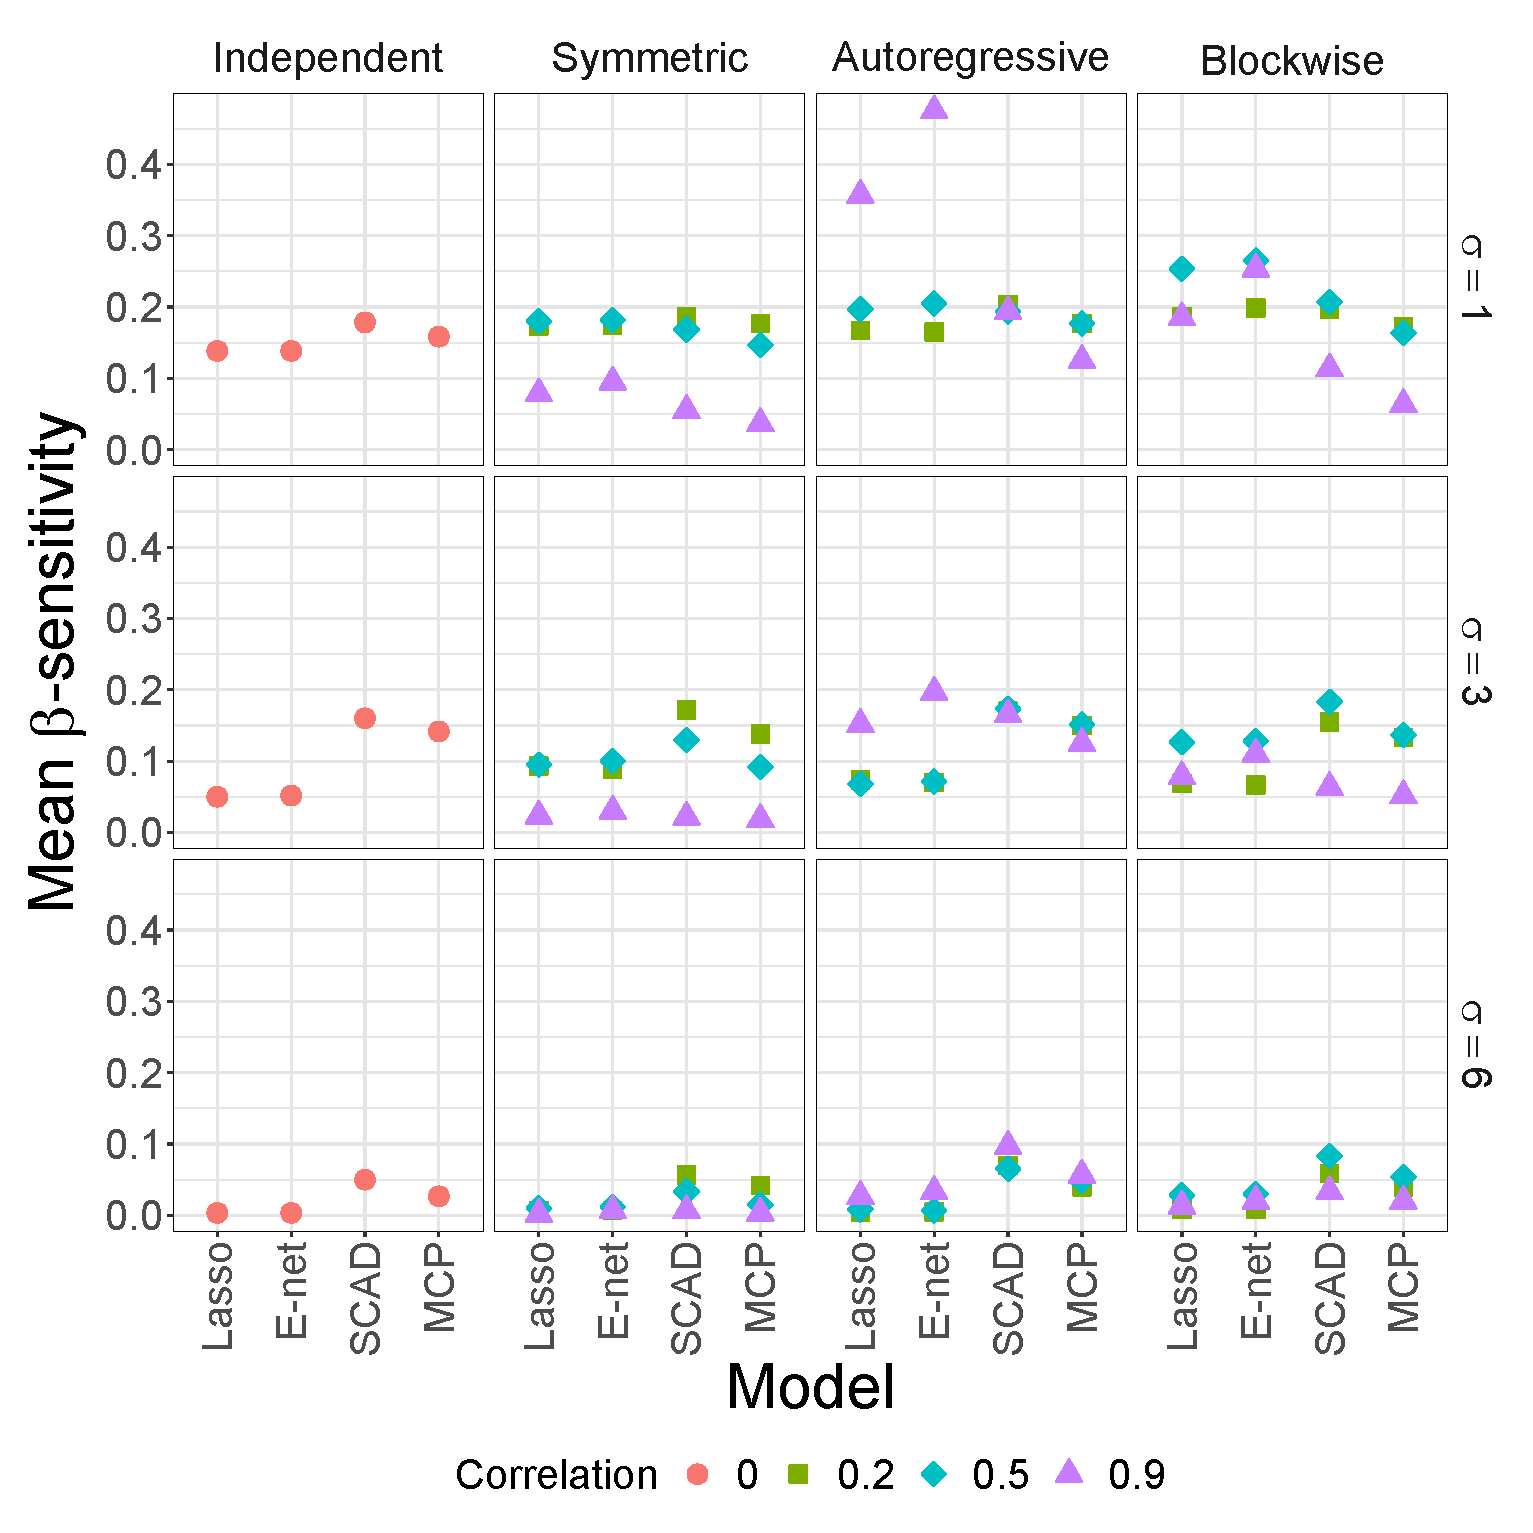
\includegraphics[width = \textwidth]{images/facet/publication_facet_sensitivity_nonlinear_50_2000.eps}
			\captionsetup{width = 0.95\textwidth}
			\caption{Average $\beta$-sensitivity for non-linear simulations when $n = 50$ and $p = 	2000$.}
			\label{fig:nonlinear-specificity}
		\end{minipage}
		\hspace{6pt}
		\begin{minipage}[t]{0.47\textwidth}
			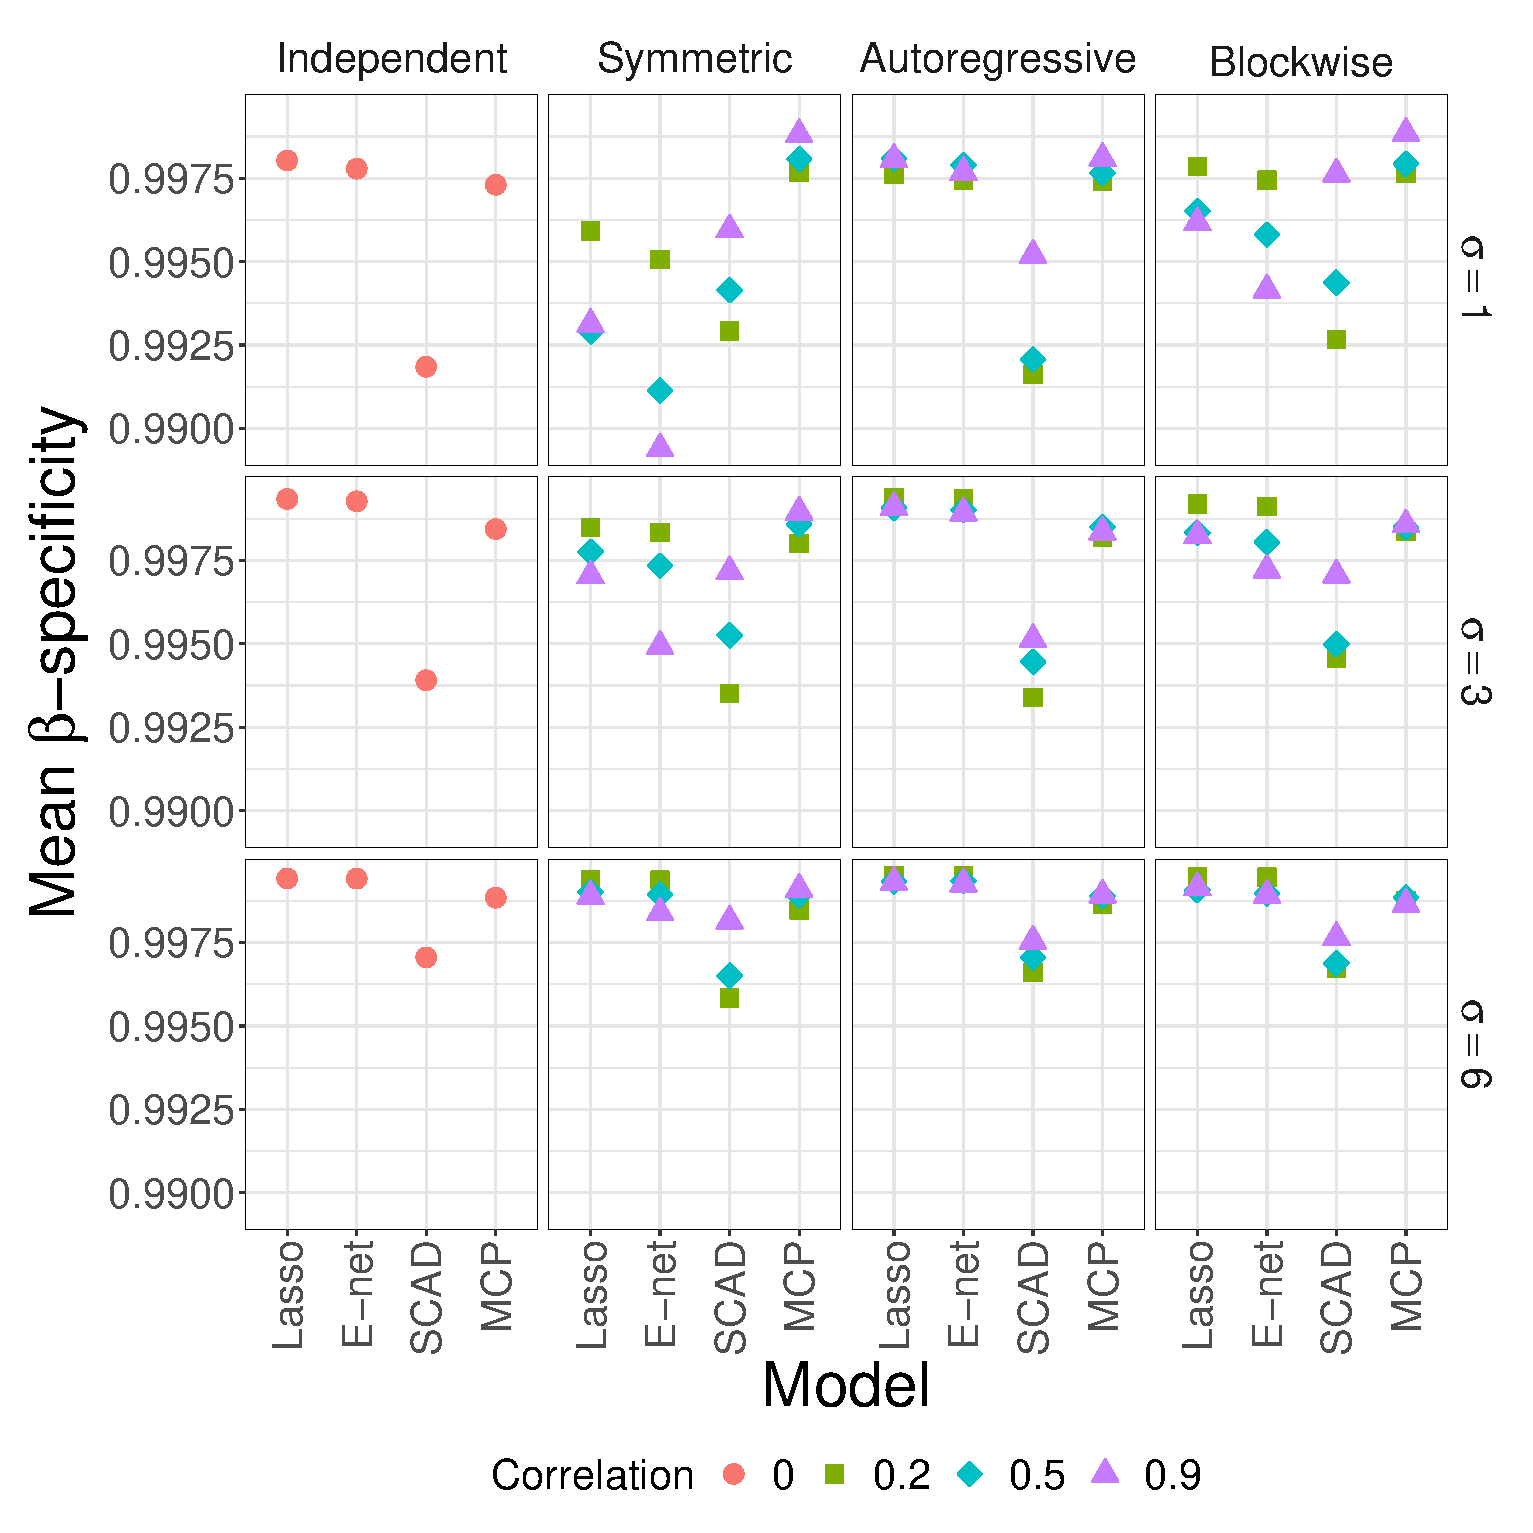
\includegraphics[width = \textwidth]{images/facet/publication_facet_specificity_nonlinear_50_2000.eps}
			\captionsetup{width = 0.95\textwidth}
			\caption{Average $\beta$-specificity for non-linear simulations when $n = 50$ and $p = 	2000$.}
			\label{fig:nonlinear-sensitivity}
		\end{minipage}
	\end{figure}
	
	\section{Empirical Data Analysis}\label{sec:empirical}
	\subsection{Details of Empirical Data}
	% outline empirical data sources and what each database is about / what we try to predict about it
	
	For empirical data, we used the Breast Cancer database from The Cancer Genome Atlas (bcTCGA). A cleaned version of the data is provided by the \lstinline!biglasso! \lstinline!R! package \cite{zeng2017biglasso}. This data set contains the gene expression data of 17323 genes from 536 patients. One of these genes is the BRCA1 gene which is among the first genes discovered that can increase the risk of breast cancer \cite{kuchenbaecker2017risks, antoniou2003average}. Mutations in BRCA 1 and BRCA 2, another gene discovered 1 year after BRCA1, are responsible for two-thirds of breast cancer cases in women \cite{deng2000roles}. Because the BRCA1 gene interacts with other genes, it is useful to find genes that interact with BRCA1 to test in further studies \cite{deng2000roles}. 
	\begin{comment}
	The distribution of the BRCA1 gene expression levels in the bcTCGA database can be seen in Figure \ref{fig:BRCA1-distribution}.
	\end{comment}
	The BRCA1 gene expression level will act as the output value in our regression analysis and the other 17322 genes will serve as predictor values.
	
	\begin{comment}
	\begin{figure}[h!]
		\centering
		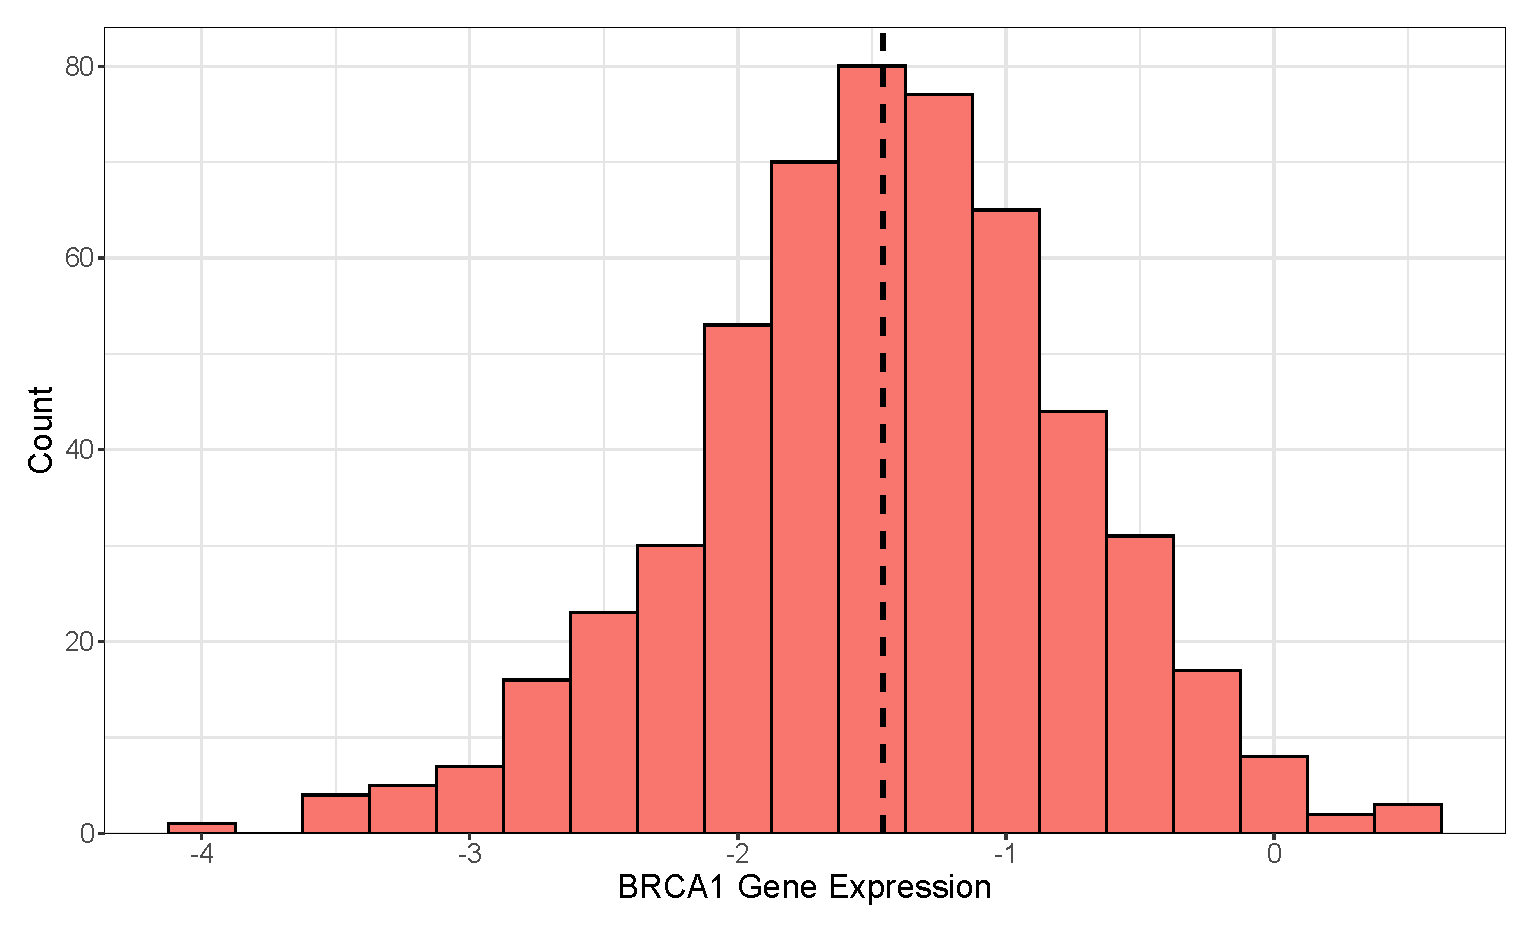
\includegraphics[width = 0.8\textwidth]{images/empirical_histogram.eps}
		\captionsetup{width = 0.8\textwidth}
		\caption{Distribution of BRCA1 gene expression levels. This is the variable that we used as the response. The mean gene expression is -1.459.}
		\label{fig:BRCA1-distribution}
	\end{figure}
	\end{comment}
	
	This data is a prime example of the large $p$ small $n$ problem where there are many more predictors than data samples. Because of this, only penalized regression and machine learning techniques can be used. This is because there are more predictors than samples which makes least squares linear regression impossible and due to the high number of predictors, subset and stepwise regression becomes too computationally expensive to be feasible. Additionally, support vector machines struggle at such a high number of predictors and resulted in stack overflow errors which made fitting support vector machines on this data impossible. It is also important to note that we do not know whether the response variable is related linearly or non-linearly to the gene expression data. This is why it is important to analyze real, empirical data when comparing mahine learning techniques since we cannot know the functional form of the data.
	
	%For analyzing the error of models fitted using this empirical data, we performed nested cross validation. Many of the models fitted used cross validation for tuning purposes to find the best input parameters. Examples of these parameters include $\lambda$ for penalized regression techniques, the number of trees and number of predictors for random forest, as well as max depth and learning rate for XGBoost. However, we also perform 5-fold cross validation before we even allow the models to tune their parameters. By doing nested cross validation, testing data is not used for training the model \textit{or} tuning model parameters. This results in a more accurate error calculation. If nested cross validation was not used, models could tune their parameters in a way that overfits the model to the testing data which would lead to artificially decreased error and invalid results.
	
	To evaluate the models, we used \textit{nested cross validation}. We first split the data into five folds. For each of these folds, we used the selected fold as a test set while the other four folds were used as a training set. We then fitted the models using cross validation on this training set, where one interior fold was used as a validation set while the other folds were used to train a model. The role of the validation set in the interior cross validation is different from the test set used in the exterior cross validation. In the interior cross validation, the validation set is used to tune hyperparameters; the model that performs best against the validation set is then chosen. On the other hand, the test set in the exterior cross validation is not used to tune hyperparameters; its only purpose is to evaluate the performance of the models chosen in the inner cross validation. Because the outer test set is not used in the model fitting or selection process, it gives an unbiased evaluation of each model's performance.
	
	We chose to use nested cross validation because it produces five models that were fitted using different subsets of the data for training and testing. If we had only fit one model, the subset of the data we choose for training and testing can have a huge impact on our findings. By using five models that are fit with different subsets of the data, we get a more accurate view of how each model performs in general. Cross validation also allows us to get an idea of how much variance each of these models has by comparing the results between different folds.
	
	The hyperparameters tuned in each of the models were the same as those tuned in the Monte Carlo simulations. For ridge, lasso, elastic-net, SCAD, and MCP, we tuned the penalty strength $\lambda$; for elastic-net, we used the hyperparameter $\alpha = 0.5$, meaning that the penalty is in between that of lasso and ridge. 
	%%%%%%%%%%%%%%%%%%%%%%%%%%%%%%%%%%%%%%%%%%%%%%%%%%%%%%%%%%%%%%%%%%%%%
	
	\subsection{Empirical Data Results}
	% Stick all the results from the linear regression models here
	Recall that we used nested cross validation when fitting models on the bcTCGA data set. This means that we fitted five models using different subsets of the data for training and testing. Figure \ref{fig:empirical_mse} below shows a plot with the training and test mean squared error for every fold of every model. The bars show the average mean squared error for the five folds. In addition, Table \ref{tab:emp_results} show the aggregated results for the train and test mean squared error.
	
	\begin{figure}[h!]
		\centering
		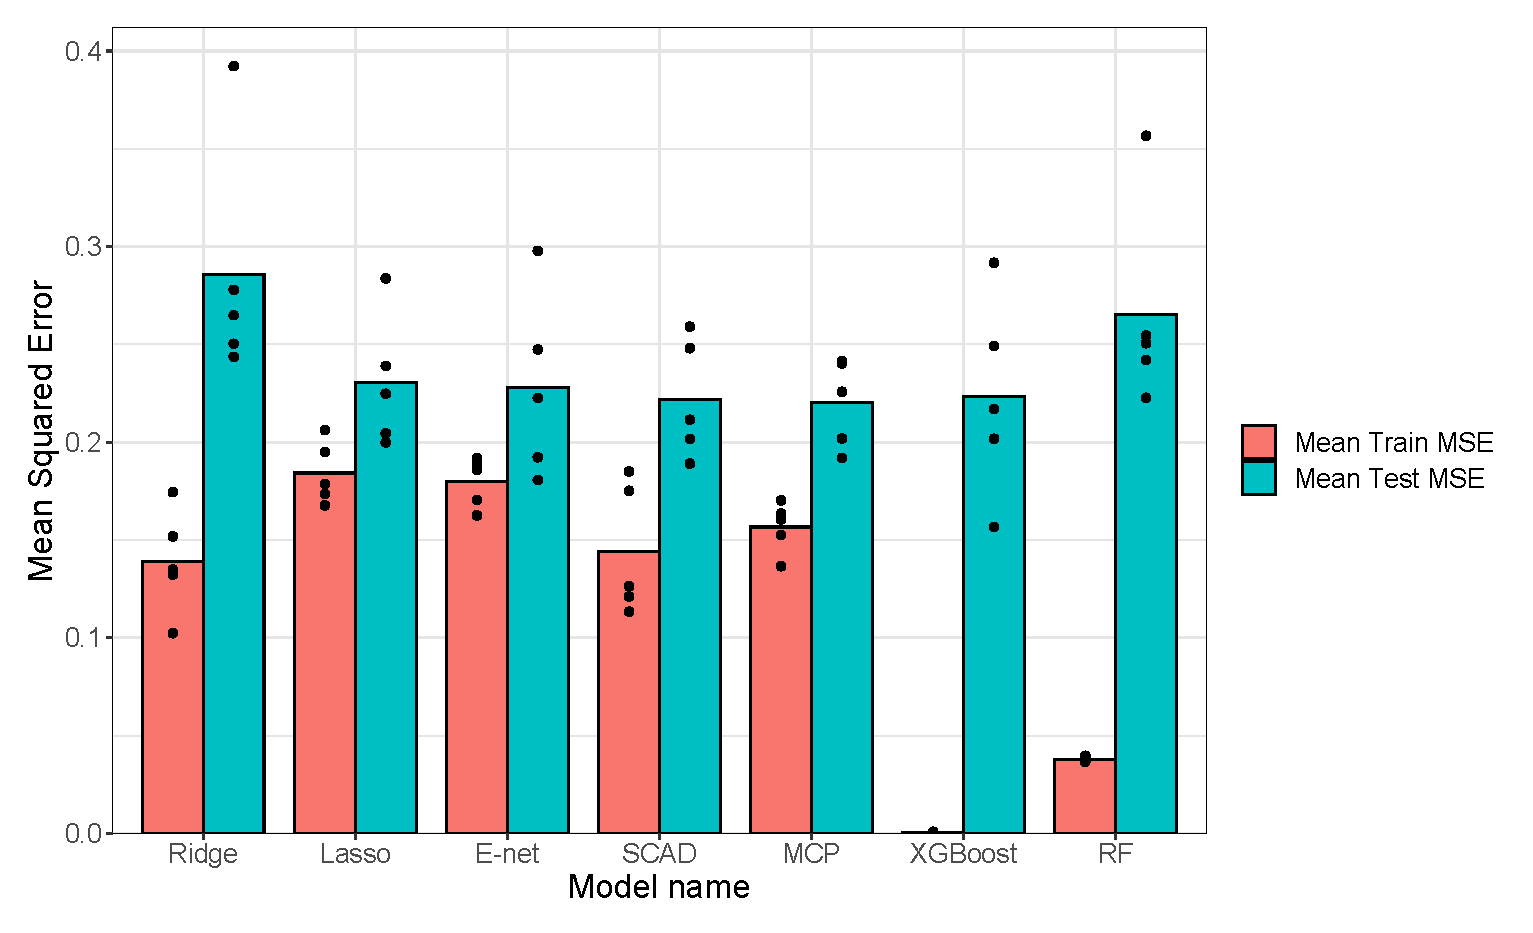
\includegraphics[width = 0.8\linewidth]{images/empirical_mse.eps}
		\captionsetup{width = 0.8\textwidth}
		\caption{Mean squared error of the models fit on the bcTCGA data set. Each point represents the mean squared error for one fold, while the bars represent the average for the five folds.}
		\label{fig:empirical_mse}
	\end{figure}
	
	\begin{table}[h!]
		\centering
		\captionsetup{width = 5in}
		\caption{Train MSE, test MSE, and runtime metrics for models fit using the bcTCGA data set.}
		\label{tab:emp_results}
		\begin{tabular}{l|ll|ll|l}
			\hline
			& \multicolumn{2}{c|}{\textbf{Train MSE}} & \multicolumn{2}{c|}{\textbf{Test MSE}} &  \\ 
			\textbf{Model } & \textbf{Average} & \textbf{SD} & \textbf{Average} & \textbf{SD} & \textbf{Average Runtime} (s) \\ 
			\hline
			Ridge  & $0.1391$ & $0.0266$ & $0.2858$ & $0.0610$ & 29.29\\
			Lasso  & $0.1842$ & $0.0159$ & $0.2304$ & $0.0337$ & 9.57\\
			E-net  & $0.1799$ & $0.0127$ & $0.2281$ & $0.0469$ & \textbf{9.41}\\
			SCAD  & $0.1442$ & $0.0333$ & $0.2218$ & $0.0303$ & 17.28\\
			MCP  & $0.1566$ & $0.0129$ & $\mathbf{0.2202}$ & $\mathbf{0.0224}$ & 15.15\\
			GBM  & $\mathbf{0.0002}$ & $\mathbf{0.0004}$ & $0.2233$ & $0.0507$ & 538.12\\
			RF  & $0.0378$ & $0.0013$ & $0.2653$ & $0.0525$ & 4906.59\\
			\hline 
		\end{tabular}
	\end{table}
	
	\begin{comment}
	The models can also be compared to each other by comparing the most important predictors selected by each model. Figure \ref{fig:venn} shows five Venn diagrams. Each diagram shows the number of variables selected by lasso, elastic-net, MCP, and random forest as the most important for each of the folds. Figure \ref{fig:venn1}, for example, shows that four of the predictors were chosen by all four models as important. For lasso, elastic-net, and MCP, a predictor is considered important if its coefficient is non-zero. For random forest, we used the 50 predictors with the highest importance score (as computed by \lstinline!randomForest!). We see that the number of predictors chosen by each model varies slightly among different folds, however, there still are common trends that are upheld between the different folds. The second fold in \ref{fig:venn2} had six predictors common to all four models, whereas the models tested in the third fold in \ref{fig:venn3} only had three.
	
	\begin{figure}[h!]
		\centering
		\begin{subfigure}[b]{0.45\textwidth}
			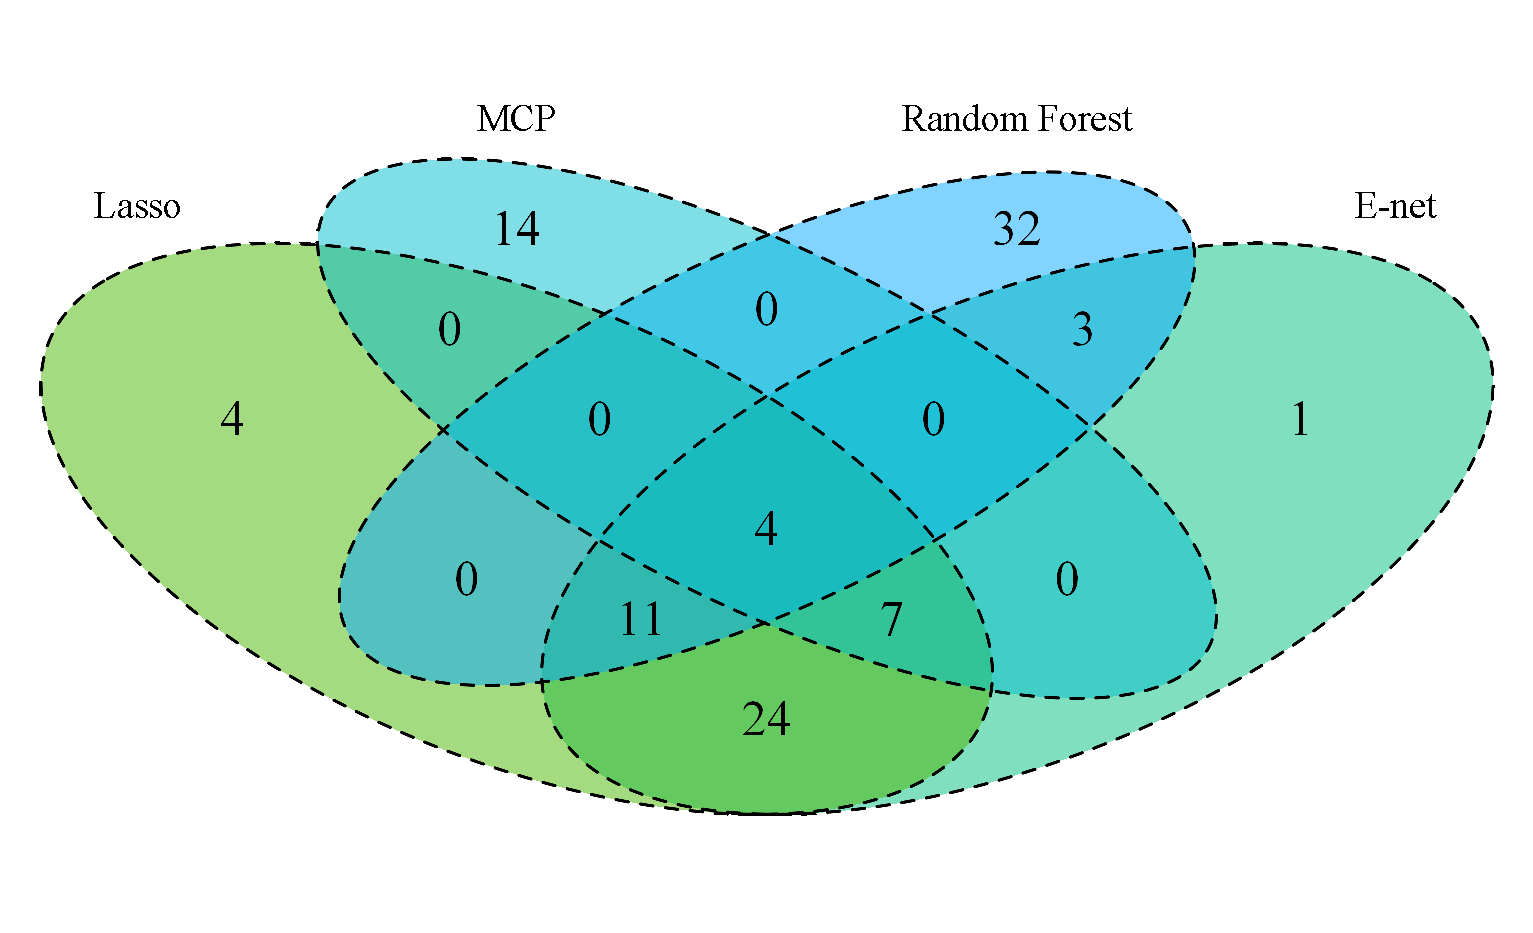
\includegraphics[width=\textwidth]{images/venn/venn1.eps}
			\subcaption{First fold}
			\label{fig:venn1}
		\end{subfigure}
		\hspace{30pt}
		\begin{subfigure}[b]{0.45\textwidth}
			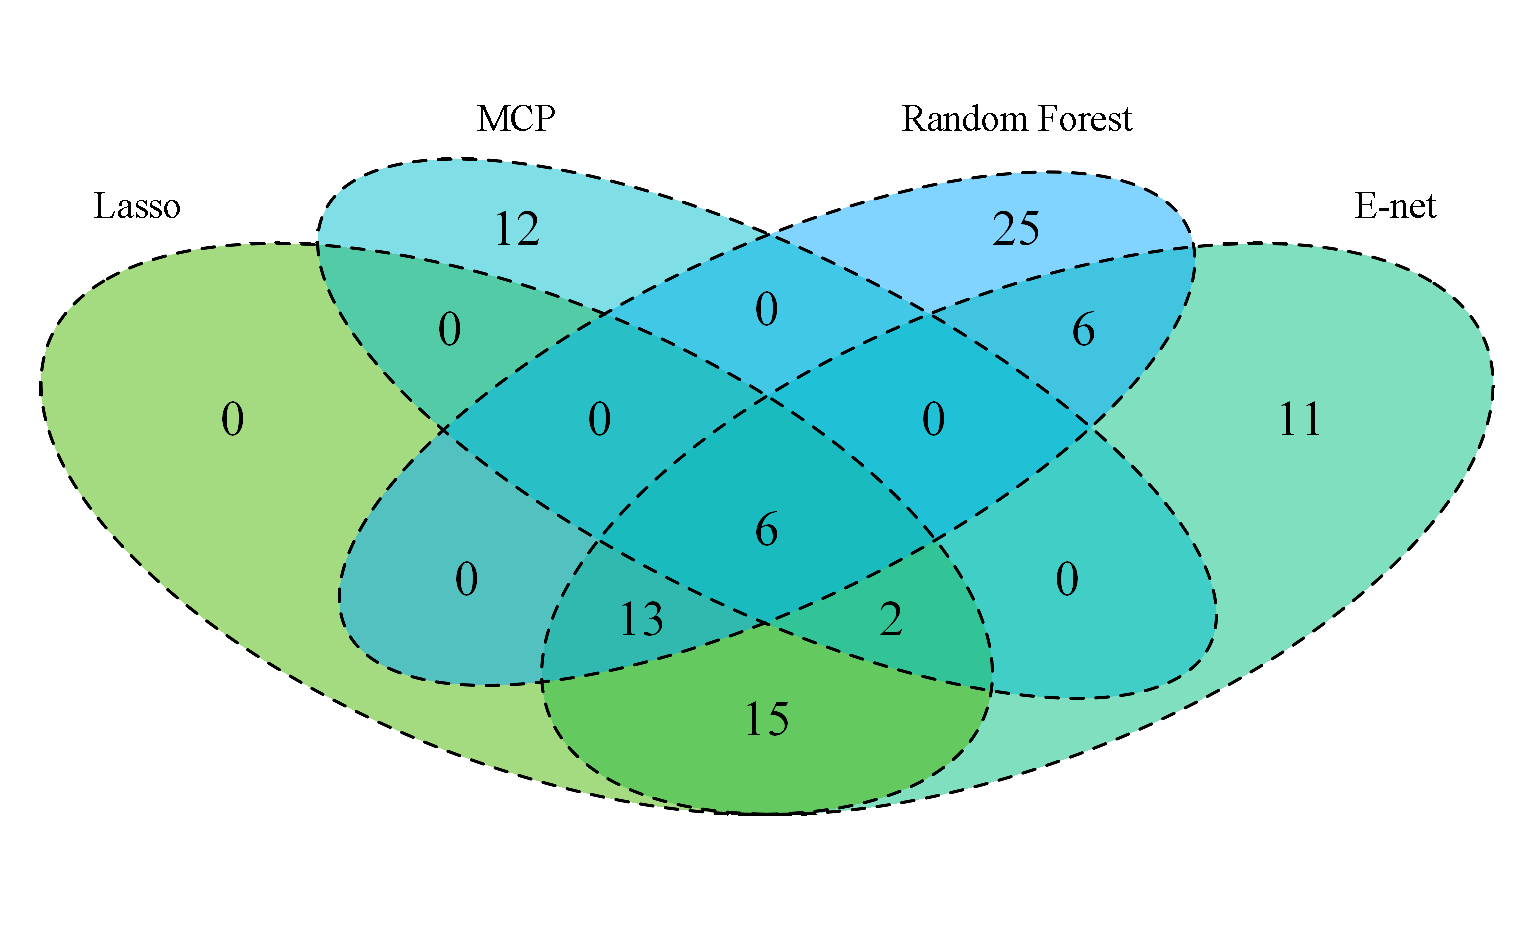
\includegraphics[width=\textwidth]{images/venn/venn2.eps}
			\subcaption{Second fold}
			\label{fig:venn2}
		\end{subfigure}
		\begin{subfigure}[b]{0.45\textwidth}
			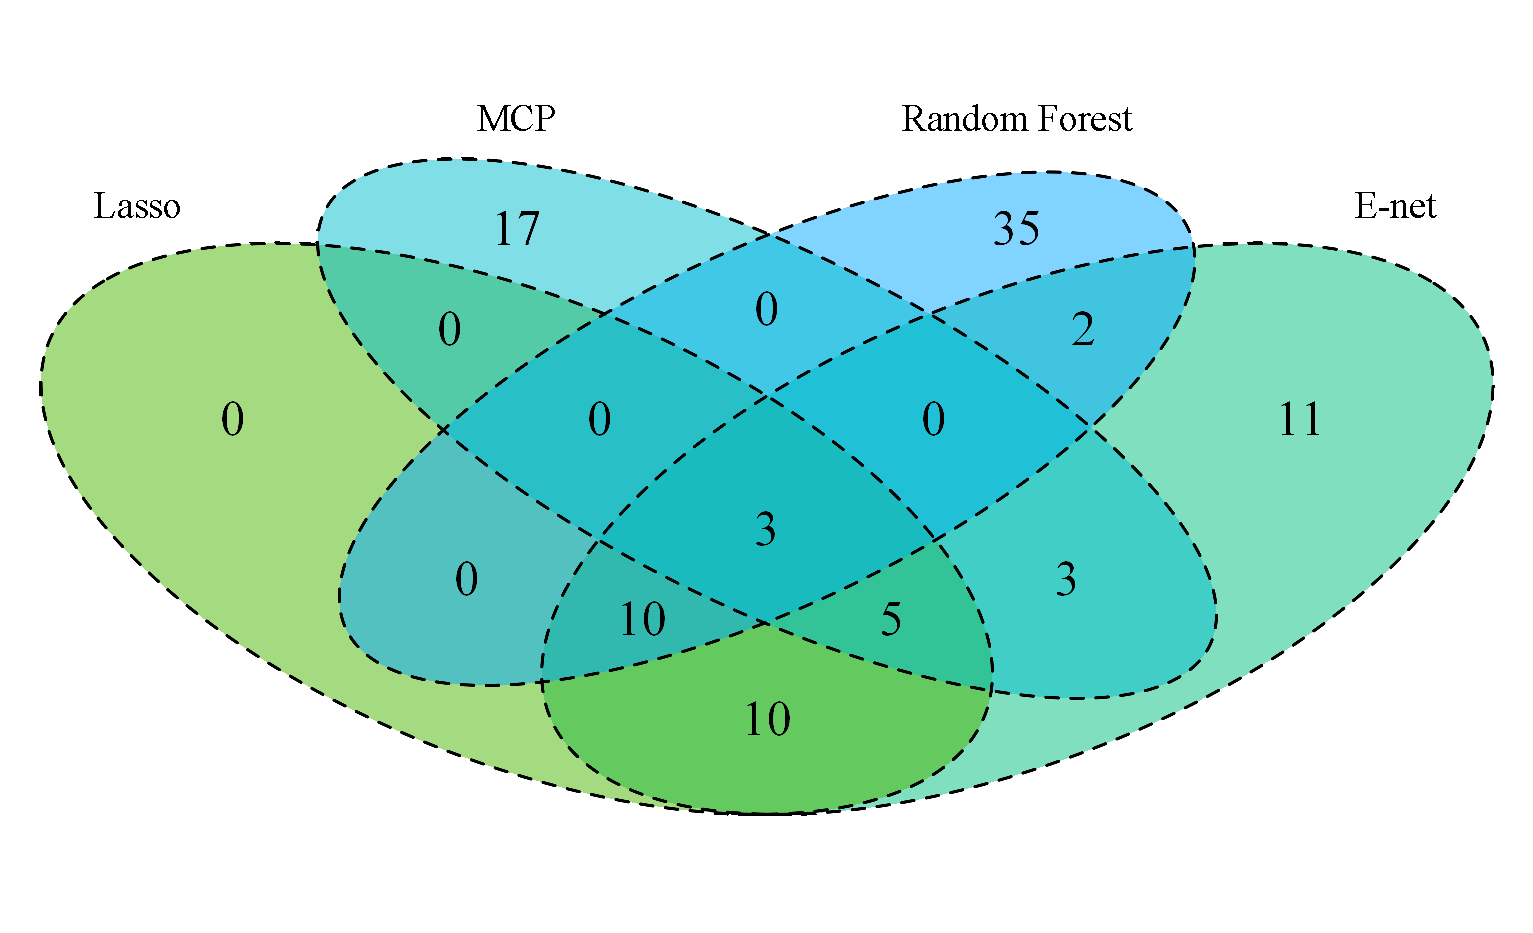
\includegraphics[width=\textwidth]{images/venn/venn3.eps}
			\subcaption{Third fold}
			\label{fig:venn3}
		\end{subfigure}
		\begin{subfigure}[b]{0.45\textwidth}
			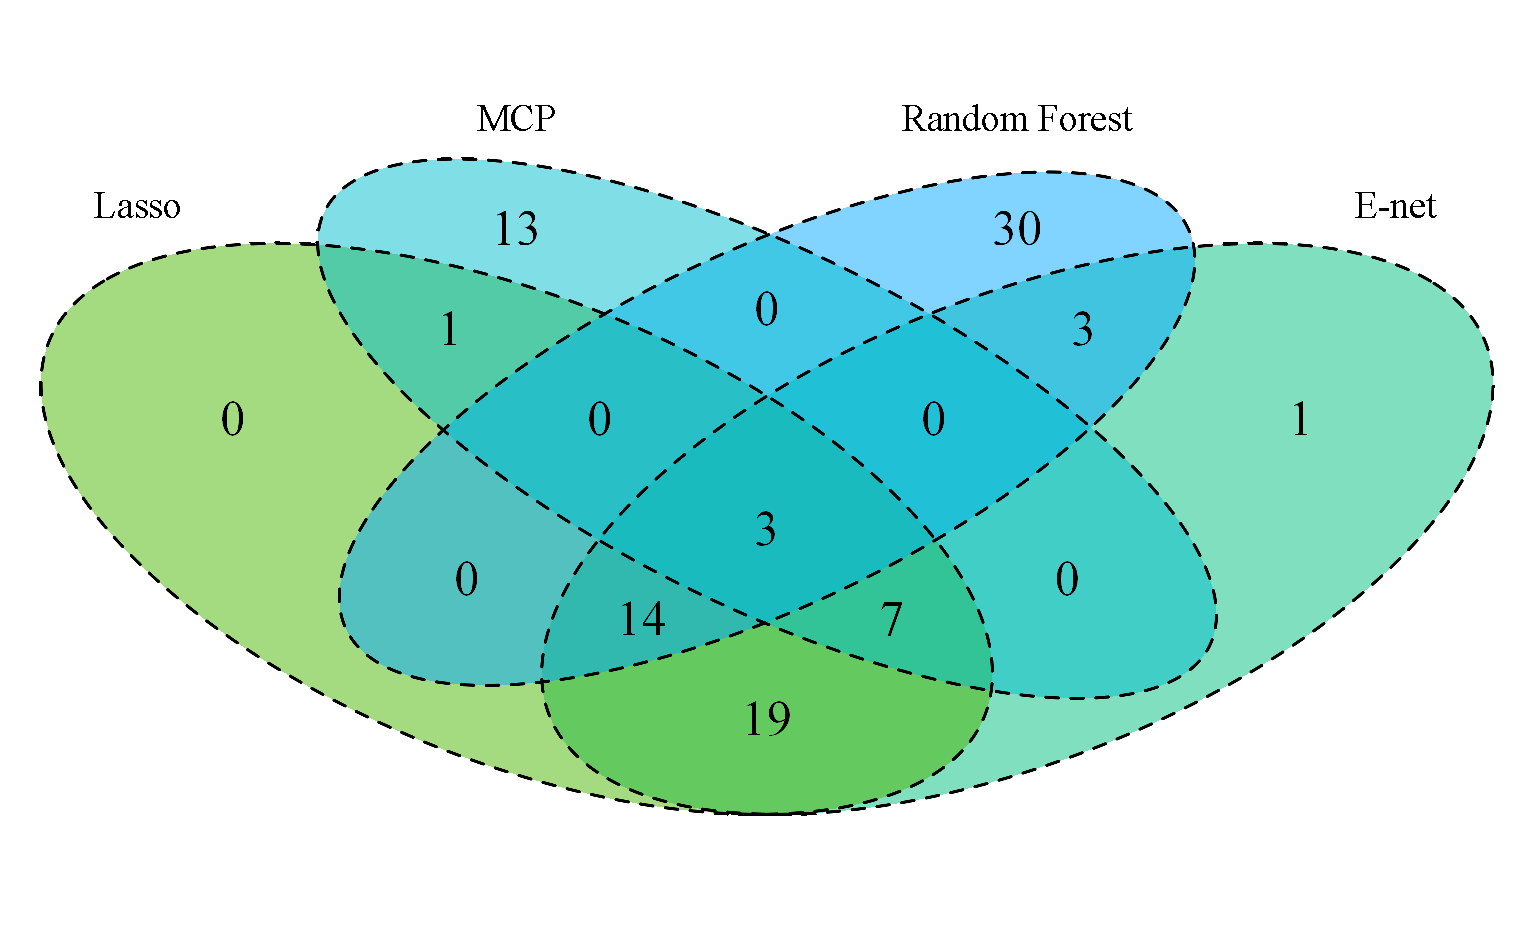
\includegraphics[width=\textwidth]{images/venn/venn4.eps}
			\subcaption{Fourth Fold}
			\label{fig:venn4}
		\end{subfigure}
		\hspace{30pt}
		\begin{subfigure}[b]{0.45\textwidth}
			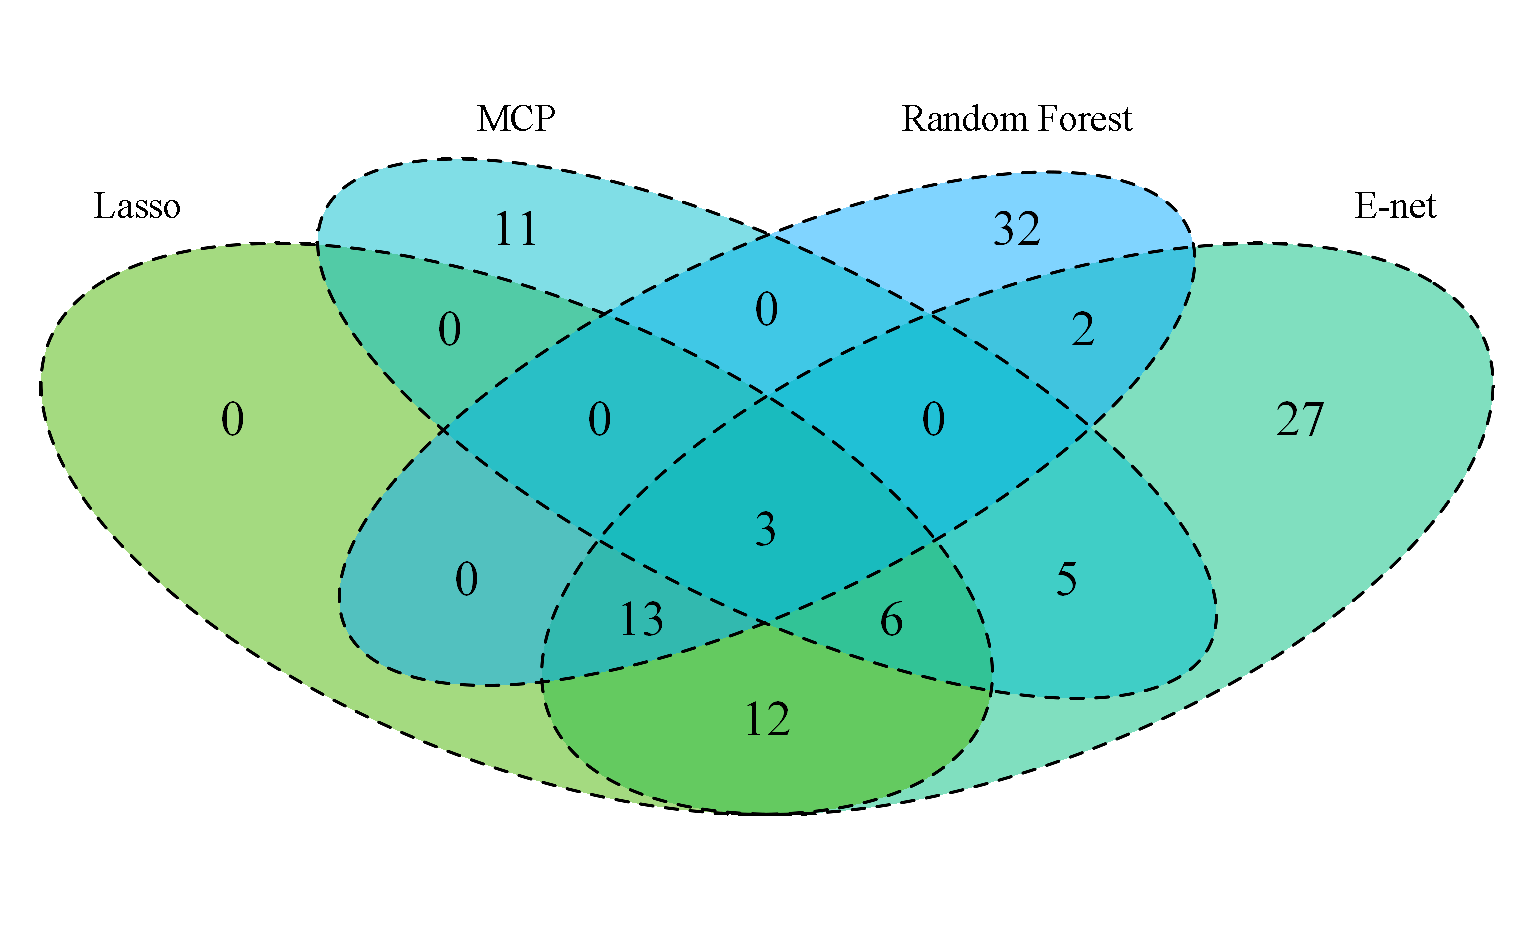
\includegraphics[width=\textwidth]{images/venn/venn5.eps}
			\subcaption{Fifth Fold}
			\label{fig:venn5}
		\end{subfigure}
		\captionsetup{width = 5in}
		\caption{Venn diagrams of the predictors selected by lasso, elastic-net, MCP, and random forest models for each of the five folds. Each number represents the number of important predictors chosen by the models that overlap the number.}
		\label{fig:venn}
	\end{figure}
	
	Several of the genes in the data set appeared in all four models for several folds, indicating that they are very strongly related to the BRCA1 gene. The most important predictor was NBR2, which appeared in all four models for all five cross validation folds. This gene is a neighbor of the BRCA1 gene and is acts as a principal tumor suppressant \cite{xiao2016nbr2}. Other significant genes that appeared in all four models for multiple folds include DTL (three folds), VPS25 (three folds), and CMTM5 (two folds). These three genes are also related to tumor suppression \cite{kobayashi2015overexpression, vaccari2005drosophila, shao2007cmtm5}.
	\end{comment}
	
	\begin{comment}
	Table \ref{tab:emp_runtimes} shows the average runtime to fit each of the models on the bcTCGA data set.
	
	\begin{table}[h!]
		\centering
		\caption{Average Runtimes for Empirical Data Models}
		\label{tab:emp_runtimes}
		\begin{tabular}{ll}
			\hline
			\textbf{Model}        & \textbf{Average Runtime} (seconds) \\ \hline
			Ridge         & 29.29               \\
			Lasso         & 9.57                \\
			E-net	      & 9.41                \\
			SCAD          & 17.28               \\
			MCP           & 15.15               \\
			GBM      	  & 538.12              \\
			RF 			  & 4906.59             \\ \hline
		\end{tabular}
	\end{table}
	\end{comment}
	
	%%%%%%%%%%%%%%%%%%%%%%%%%%%%%%%%%%%%%%%%%%%%%%%%%%%%%%%%%%%%%%%%%%%%%
	\newpage
	\section{Discussion}\label{sec:discussion}
	
	We first discuss in detail our findings from the simulations where $n = 50$ and $p = 2000$. Then, we discuss some of the broader results that arose for other values of $n$ and $p$. We defer the reader to our supplementary document to see the figures and tables for the remaining simulations. Lastly, we discuss findings from the empirical analysis.
	
	% discussion of findings, future work, and contributions
	Figure \ref{fig:linear-test-mse} indicates that the best-performing algorithms on Model 1 were SCAD and MCP. 
	\begin{comment}
	The wrapper methods that used BIC performed better than SCAD and MCP when $n = 1000$ and $p = 10$, but could not be used in the high dimensional case where $n = 50$ and $p = 2000$. Lasso, elastic-net, and the wrapper methods with AIC all had low test mean squared errors as well. Ridge performed the worst out of all the linear models. The non-linear models also performed very badly on test data.
	\end{comment}
	Most other linear models considered performed relatively well, with ridge being an exception. The non-linear models all had high test MSEs, but performed much better when the correlation between predictors was large.
	
	In Model 2, the linear models all performed similarly well on test data. Unlike with the linear response, the non-linear models outperformed the linear models with a non-linear response function. This is especially apparent when the correlation between predictors was 0.9, where XGBoost and random forest models performed incredibly well.
	
	One possible explanation for this phenomenon is that the XGBoost and random forest models are less influenced by the random error when the correlation is large. For example, when the correlation is zero, only a fraction of the decision trees generated in each random forest will contain any of the important predictors; many of the trees will instead be fit using only predictors that are unrelated to the response. This means that the random forest model is fitting with a large amount of noise. On the other hand, when the correlation is high, all of the trees will contain predictors that are correlated with the  predictors with non-zero coefficients. As a result, none of the trees will truly be fitting on just random error. Similarly, for XGBoost models, the strong correlation may make it more difficult to fit using just the random noise.
	
	\begin{comment}
	Notice that all the linear models except for ridge had a test mean squared error that was approximately equal to $\sigma^2$, the square of the random error. This indicates that these models had low bias and low variance, since most of their error was due to the random noise. On the other hand, ridge regression and the machine learning models had a test mean squared error that was much higher than $\sigma^2$, indicating that these models either had high bias or high variance.
	\end{comment}
	
	\begin{comment}
	Now, consider the training mean squared error results from Figures \ref{fig:linear-train-mse-1000-10} and \ref{fig:linear-train-mse-50-2000}. We see that training error for the linear models was roughly equal to the test error. This indicates that these models did not overfit to the training data. On the other hand, the non-linear models have far lower training mean squared errors than test errors. In particular, random forest models almost perfectly fit to the training data when $n = 1000$ and $p = 10$, while gradient boosting made an almost perfect fit when $n = 50$ and $p = 2000$.
	\end{comment}
	
	If we compare the MSE between the training data and test data for both Model 1 and Model 2, we notice that the linear models had almost the same MSE in both cases. This demonstrates that these models have a very low variance; that is, the linear models are not very sensitive to the training data used. This is what makes penalized linear models useful in high-dimensional situations. On the other hand, the non-linear models had very low training MSEs (sometimes even lower than MCP and SCAD). This indicates that the non-linear models are overfitting, since their performance on test data is significantly worse.
	
	Ridge regression, which performed badly on both training data and test data, was likely restricted by its penalty function and its inability to perform variable selection. Recall that three out of the five non-zero coefficient values chosen in the linear response function were greater than one. Because the penalty function for ridge squares each coefficient, ridge was very strongly discouraged from selecting coefficient estimates close to the true non-zero coefficient values. Furthermore, because ridge regression cannot set coefficients to zero, its coefficient estimates for the true non-zero coefficients were likely even smaller because unimportant predictors were given non-zero coefficient estimates. As a result, ridge regression was unable to predict the true coefficient values as well as the other linear models.
	
	\begin{comment}
	Another note about ridge regression is that it was more strongly affected by correlation between predictors when $n = 1000$ and $p = 10$, as seen in Figure \ref{fig:test-mse-1000-10}. The other linear models, which could set coefficients to zero, were likely able to eliminate unimportant predictors even though they were correlated with the important predictors. Ridge regression, unable to eliminate these unimportant predictors, may have instead given larger coefficient estimates to the incorrect predictors.
	
	Interestingly, the test mean squared error for random forest and support vector machine models improved as the correlation between predictors was increased. Figures \ref{fig:test-mse-1000-10} and \ref{fig:test-mse-50-2000} show that the test mean squared error for random forest and support vector machines decreased when correlation was increased. On the other hand, XGBoost was unaffected by an increase in the correlation value.
	\end{comment}
	
	Note that changing the standard deviation of the random error seems to affect the mean squared errors of all the models equally. In addition, the correlation structure appears to have little influence on the training or test mean squared error.
	
	Now, we will consider the $\beta$-sensitivity and $\beta$-specificity results for the linear models that could perform variable selection. With the linear response, SCAD and MCP had the highest $\beta$-sensitivities for small correlation values but the lowest $\beta$-sensitivities when the correlation is high. This appears to indicate that SCAD and MCP are particularly weak at determining important predictors when variables are highly correlated. Looking at the $\beta$-specificity under the linear response, we see that MCP was by far the best model. It was able to identify nearly all of the predictors that needed coefficients of zero. The other linear models performed slightly worse than MCP.
	
	With the non-linear response function, we notice that none of the linear models showed any particular strengths when considering the $\beta$-sensitivity and $\beta$-specificity. The linear models appear to set almost all of the coefficients to zero, indicating that they all did a poor job of identifying important predictors.
	
	\begin{comment}
	Looking at the $\beta$-specificity results from Figures \ref{fig:linear-specificity-1000-10} and \ref{fig:linear-specificity-50-2000}, we see that lasso, elastic-net, and the BIC wrapper methods had the highest $\beta$-specificity when $n = 1000$ and $p = 10$. When $n = 50$ and $p = 2000$, lasso and elastic-net had must lower $\beta$-specificity values compared to SCAD and MCP.
	
	Another interesting result to note is that for both low-dimensional and high-dimensional settings, when the correlation between predictors increased, the $\beta$-specificity for SCAD and MCP typically increased. For elastic-net, a higher correlation caused the $\beta$-specificity to decrease when $n = 1000$ and $p = 10$; however, when $n = 50$ and $p = 2000$, the $\beta$-specificity of elastic-net depends heavily on the correlation structure. For a symmetric compound correlation structure, elastic-net had a much lower $\beta$-specificity as correlation increased. For an autoregressive or blockwise correlation structure, a higher correlation increased the $\beta$-specificity for elastic-net. This means that lasso and elastic-net have trouble identifying non-zero coefficients when all $p = 2000$ predictors are correlated to each other, while SCAD and MCP could handle this situation well.
	
	Overall, we see that the ability for the penalized models to correctly identify whether coefficients are non-zero depends on how predictors are correlated with one another. However, the standard deviation of the random error does not appear to be too impactful on $\beta$-sensitivity or $\beta$-specificity.
	
	% One interesting observation is that many of the models did better at avoiding estimating coefficients as non-zero that were actually zero when the correlation was large. This is most evident in Figure \ref{fig:fp-50-2000}, which shows that the number of false predictions typically decreased as the correlation increases in the case where $n = 50$ and $p = 2000$. One possible explanation for this comes from the fact that the predictors chosen to be non-zero are close to each other ($\beta_0$, $\beta_1$, $\beta_2$, $\beta_5$ and $\beta_6$ were chosen to be non-zero). As a result, having a strong correlation means that these predictors are more closely related to one another, so the regression algorithms are more likely to identify one or more of these predictors as significant. However, this correlation makes it harder for the model to identify which particular predictors are related to the response; figure \ref{fig:tp-50-2000} shows that as the correlation increases, the penalized models recognize less of the non-zero coefficients as being non-zero.
	
	% To further support this idea, notice in figure \ref{fig:fp-50-2000} that the number of false predictions decreases as the correlation increases mainly when the correlation structure is autoregressive or blockwise; when the correlation structure is symmetric compound, lasso and elastic-net do not improve as the correlation increases. This could be because symmetric compound correlation makes all of the predictors correlated with one another, whereas autoregressive and blockwise correlation make nearby predictors correlated with one another. By increasing the correlation with a symmetric compound structure, lasso and elastic-net are more likely to estimate more unimportant predictors as having non-zero coefficients because all of the predictors are correlated with the important predictors. On the other hand, with autoregressive and blockwise correlation, less of the unimportant predictors are correlated with the important predictors but the correlation between the important predictors stays the same. As a result, the models are less likely to incorrectly assume that unimportant predictors are important when the correlation structure is autoregressive or blockwise.
	
	Although wrapper methods and penalized regression models were the evident winners in this simulation study, it is worth noting that the non-linear models suffered from a few unfair disadvantages. For one, the simulated data assumed that there was a linear relationship between the predictors and response, which meant that the linear models were almost unbiased. The non-linear models were relatively more biased because they did not assume a linear relationship.
	\end{comment}
	
	Now, we will discuss some results that broadly applied to our simulations, rather than just focusing on the $n = 50$ and $p = 2000$ case. Again, these results can be found at \href{https://github.com/connor-shrader/reu-2021}{github.com/connor-shrader/reu-2021}.
	
	The subset selection methods generally had a similar MSE on training and test data as SCAD and MCP. This makes them fairly well-performing linear models; however, these models are computationally infeasible to use with a large number of predictors. The subset selection methods that used BIC as a stopping condition typically had higher $\beta$-sensitivity and $\beta$-specificity values. This is expected since BIC will choose fewer non-zero coefficients than AIC.
	
	The linear models consistently had a lower MSE on test data than the non-linear models with the linear response function. With a non-linear response function, the linear models were competitive with non-linear models when $p$ was sufficiently large. In cases where $p$ was relatively small compared to $n$, the non-linear models dominated.
	
	The linear models consistently had difficulty identifying important predictors with the non-linear response function. This is somewhat expected, since many of the predictors in the non-linear response did not use linear terms. Nonetheless, this shows that the linear models can be rather unreliable when estimating coefficients as non-zero when the response is not linear.
	
	\begin{comment}
	Another disadvantage for the non-linear models is that they can be controlled by many different hyperparameters, but we only considered a couple for each model. This was out of necessity; it would have been infeasible to fit models using more hyperparameters given the number of simulations that had to be run. If more hyperparameters could be included, then the performance of the non-linear models may have improved. At the same time, the more comprehensive tuning of several hyperparameters could act as a double edged sword in that it could increase the overfitting of these models. More hyperparameter tuning could lead a model to pick hyperparameters that fit the training data very precisely, but at the expense of increased testing error and computational cost.
	\end{comment}
	
	In our empirical data study, SCAD and MCP also maintained the lowest testing mean squared error among the tested models. This can be seen in Figure \ref{fig:empirical_mse} and Table \ref{tab:emp_results}. Furthermore, the mean squared error MCP had a relatively low standard deviation across the five folds. 
	\begin{comment}
	This may be due in part to the fact that MCP consistently selected the fewest number of predictors compared to Lasso and Elastic Net as shown by the Venn diagrams in Figure \ref{fig:venn}. Because this empirical data most likely contains multicollinearity, the fact that MCP selects fewer predictors may have helped to reduce overfitting. This is consistent with results from the Monte Carlo simulations which indicate that MCP performed better than its counterparts in multicollinear environments.
	\end{comment}
	
	\begin{comment}
	An interesting result was how few predictors were selected between all four models. It would be expected that the most important predictors would be chosen by all four models, but only three to six predictors were selected in common by all the models. Between MCP, Lasso, and Elastic Net, there were slightly more selected predictors in common, but these still were much less than expected. This is most likely because MCP is very different from the other regression techniques in that it uses non-convex optimization and thus selected many predictors that were different from all the other models. Since MCP had a much higher $\beta$-sensitivity and $\beta$-specificity rate compared to the other models as determined in the Monte Carlo simulations, it can be assumed that many of these predictors solely selected by MCP were significant predictors that were missed by the other models. This could have been another reason why MCP performed the best out of all the fitted models on the empirical data.
	\end{comment}
	
	MCP also maintained the lowest testing MSE standard deviation for the empirical data as seen in Figure \ref{tab:emp_results}. This is to be expected given the bias/variance tradeoff. Because MCP selects fewer predictors than the other models, it incurs greater bias but while also lessening variance. By definition, this means that MCP is less sensitive to changes in training data, such as changes in training data due to 5-fold cross validation. 
	
	The penalized regression models performed exceptionally faster than random forest and XGBoost as documented in Table \ref{tab:emp_runtimes}. On average, Lasso and Elastic Net ran approximately 56x faster than XGBoost and 510x faster than random forest. MCP and SCAD ran approximately 30x faster than XGBoost and 290x faster than random forest. This provides a significant advantage to the penalized regression techniques, especially given that MCP and other penalized techniques performed better than random forest and XGBoost. 
	
	We conclude with the following summary of findings:
	\begin{itemize}
		\item In Model 1, penalized linear models have a lower MSE on test data than non-linear models.
		\item Non-linear models had a lower MSE on training data than linear models in almost all the simulations.
		\item In Model 1, penalized linear models generally have a slightly higher test MSE when $p > n$ when compared to non-linear models. When $n > p$, the linear models had a significantly higher test MSE.
		\item Among the linear models, SCAD and MCP generally had the lowest test MSE. OLS and ridge regression usually had the highest.
		\item SCAD and MCP tended to be more picky about the variables they selected compared to other linear models, especially when the correlation among predictors was high. This is evidenced by these models having a lower $\beta$-sensitivity and higher $\beta$-specificity.
		\item The linear models struggled to identify important predictors in Model 2.
		\item The standard deviation of the random error did not have any broad qualitative effects on the results, nor did the correlation structure.
		\item In the empirical analysis, SCAD and MCP performed the best and had the lowest testing MSE among tested models.
		\item Penalized regression models ran substantially faster the than non-linear machine learning models in Model 1, Model 2, and the empirical data analysis.
	\end{itemize}
	
	
	\section{Conclusion}\label{sec:conclusion}
	
	% what are our contributions, why is what we did important?
	% we have a comprehensive analysis of 21 models in 270 different environments. Allows for comprehensive comparison and gives guidance to data scientists as to which model they should use for their research
	% empirical data methods show the important uses of penalized regression in environmental, biological, and etc. data
	There is a severe lack of comprehensive testing comparing traditional machine learning methods such as random forest, gradient boosting, and support vector machines with penalized regression. Our paper bridges the divide between the machine learning and statistical fields in which these two types of models exist in. Testing using Monte Carlo simulations and empirical data has not been tested by other researchers with as many different environments and models.
	
	These comparisons have shown that penalized regression should be added to the toolbox of any data scientist. In addition to performing better with less error than traditional machine learning techniques, penalized regression is much less computationally expensive. Additionally, in scenarios such as the empirical data study outlined earlier, penalized regression techniques can help determine the relationship between predictors and a response value. In such cases, the ability to determine these relationship can be more important than the predictive performance of a model.
	
	We could also run Monte Carlo simulations where the response is categorical rather than numerical. This could be used to study how penalized regression performs when used for classification data, which is the most common case for high dimensional data sets.
	
	In the future, it may be useful to develop a hybrid technique between random forest and penalized regression. This method would harness the power of ensemble learning, while still being able to perform variable selection and would hopefully perform better than either random forest or penalized regression methods individually. There are some models such as SREEMforest \cite{capitaine2021random} which conduct variable selection, however, these models use wrapper methods and variable importance which can be computationally expensive and do not inherently eliminate insignificant variables the same way penalized regression does. Given that random forest models are already very slow, performing additional stepwise selection may result in an exponentially slower runtime. Thus, it is important that inherent variable selection methods such as penalized regression methods are utilized in ensemble methods.
	
	\section{Acknowledgments}
	
	This research was conducted as a part of the North Carolina A\&T State University and Elon University Joint Summer REU Program in Mathematical Biology and was funded by the National Science Foundation DMS\# 1851957/1851981.
	
	The results here are in part based upon data generated by the TCGA Research Network: \href{https://www.cancer.gov/tcga}{https://www.cancer.gov/tcga}.
	
	We would also like to thank Dr. Luke and Dr. Yokley and Yang Xue for their guidance throughout the research process.
	
	\bibliographystyle{plain-lf}
	{\footnotesize
	\bibliography{references}
	}
	\begin{comment}
	\newpage
	\appendix
	\section{Full Result Tables}\label{app:full-results}
	The following pages contain the full table of Monte Carlo simulation results. Each table corresponds to one of the figures in Section \ref{sec:evaluating-model-results}. The full results as well as relevant R code can be accessed through our \href{https://github.com/connor-shrader/reu-2021}{Github repository}.
	
	\setlength{\tabcolsep}{3pt}
	
	{\tiny
		\begin{landscape}
			\centering
			\captionsetup{width = 6in}
			\captionof{table}{Mean and standard deviation of the mean squared error on training data when $n = 1000$ and $p = 10$. See Figure \ref{fig:linear-train-mse-1000-10} for the corresponding plot.}
			\label{tab:linear-train-mse-1000-10}
			\begin{tabular}{llllllllllllllllllllll}
	\hline
	& & \multicolumn{20}{l}{type} \\ 
	& & \multicolumn{2}{l}{independent} & \multicolumn{6}{l}{symmetric} & \multicolumn{6}{l}{autoregressive} & \multicolumn{6}{l}{blockwise} \\ 
	& & \multicolumn{2}{l}{corr} & \multicolumn{6}{l}{corr} & \multicolumn{6}{l}{corr} & \multicolumn{6}{l}{corr} \\ 
	& & \multicolumn{2}{l}{0} & \multicolumn{2}{l}{0.2} & \multicolumn{2}{l}{0.5} & \multicolumn{2}{l}{0.9} & \multicolumn{2}{l}{0.2} & \multicolumn{2}{l}{0.5} & \multicolumn{2}{l}{0.9} & \multicolumn{2}{l}{0.2} & \multicolumn{2}{l}{0.5} & \multicolumn{2}{l}{0.9} \\ 
	& & \multicolumn{2}{l}{train.mse} & \multicolumn{2}{l}{train.mse} & \multicolumn{2}{l}{train.mse} & \multicolumn{2}{l}{train.mse} & \multicolumn{2}{l}{train.mse} & \multicolumn{2}{l}{train.mse} & \multicolumn{2}{l}{train.mse} & \multicolumn{2}{l}{train.mse} & \multicolumn{2}{l}{train.mse} & \multicolumn{2}{l}{train.mse} \\ 
	st.dev & model.name & Mean & SD & Mean & SD & Mean & SD & Mean & SD & Mean & SD & Mean & SD & Mean & SD & Mean & SD & Mean & SD & Mean & \multicolumn{1}{l}{SD} \\ 
	\hline
	1 & OLS  & $\phantom{0}0.99$ & $0.04$ & $\phantom{0}0.99$ & $0.04$ & $\phantom{0}0.99$ & $0.04$ & $\phantom{0}0.99$ & $\phantom{0}0.04$ & $\phantom{0}0.99$ & $0.04$ & $\phantom{0}0.99$ & $0.04$ & $\phantom{0}0.99$ & $0.04$ & $\phantom{0}0.99$ & $0.04$ & $\phantom{0}0.99$ & $0.04$ & $\phantom{0}0.99$ & $0.04$ \\
	& AIC B  & $\phantom{0}1.00$ & $0.04$ & $\phantom{0}1.00$ & $0.04$ & $\phantom{0}1.00$ & $0.04$ & $\phantom{0}1.00$ & $\phantom{0}0.04$ & $\phantom{0}1.00$ & $0.04$ & $\phantom{0}1.00$ & $0.04$ & $\phantom{0}0.99$ & $0.04$ & $\phantom{0}1.00$ & $0.04$ & $\phantom{0}0.99$ & $0.04$ & $\phantom{0}1.00$ & $0.04$ \\
	& BIC B  & $\phantom{0}1.00$ & $0.04$ & $\phantom{0}1.00$ & $0.04$ & $\phantom{0}1.00$ & $0.04$ & $\phantom{0}1.00$ & $\phantom{0}0.04$ & $\phantom{0}1.00$ & $0.04$ & $\phantom{0}1.00$ & $0.04$ & $\phantom{0}1.00$ & $0.04$ & $\phantom{0}1.00$ & $0.04$ & $\phantom{0}1.00$ & $0.04$ & $\phantom{0}1.00$ & $0.04$ \\
	& AIC SB  & $\phantom{0}1.00$ & $0.04$ & $\phantom{0}1.00$ & $0.04$ & $\phantom{0}1.00$ & $0.04$ & $\phantom{0}1.00$ & $\phantom{0}0.04$ & $\phantom{0}1.00$ & $0.04$ & $\phantom{0}1.00$ & $0.04$ & $\phantom{0}0.99$ & $0.04$ & $\phantom{0}1.00$ & $0.04$ & $\phantom{0}0.99$ & $0.04$ & $\phantom{0}1.00$ & $0.04$ \\
	& BIC SB  & $\phantom{0}1.00$ & $0.04$ & $\phantom{0}1.00$ & $0.04$ & $\phantom{0}1.00$ & $0.04$ & $\phantom{0}1.00$ & $\phantom{0}0.04$ & $\phantom{0}1.00$ & $0.04$ & $\phantom{0}1.00$ & $0.04$ & $\phantom{0}1.00$ & $0.04$ & $\phantom{0}1.00$ & $0.04$ & $\phantom{0}1.00$ & $0.04$ & $\phantom{0}1.00$ & $0.04$ \\
	& AIC F  & $\phantom{0}1.00$ & $0.04$ & $\phantom{0}1.00$ & $0.04$ & $\phantom{0}1.00$ & $0.04$ & $\phantom{0}1.00$ & $\phantom{0}0.04$ & $\phantom{0}1.00$ & $0.04$ & $\phantom{0}1.00$ & $0.04$ & $\phantom{0}1.00$ & $0.04$ & $\phantom{0}1.00$ & $0.04$ & $\phantom{0}1.00$ & $0.04$ & $\phantom{0}1.00$ & $0.04$ \\
	& BIC F  & $\phantom{0}1.00$ & $0.04$ & $\phantom{0}1.00$ & $0.04$ & $\phantom{0}1.00$ & $0.04$ & $\phantom{0}1.00$ & $\phantom{0}0.04$ & $\phantom{0}1.00$ & $0.04$ & $\phantom{0}1.00$ & $0.04$ & $\phantom{0}1.00$ & $0.04$ & $\phantom{0}1.00$ & $0.04$ & $\phantom{0}1.00$ & $0.04$ & $\phantom{0}1.00$ & $0.04$ \\
	& AIC SF  & $\phantom{0}1.00$ & $0.04$ & $\phantom{0}1.00$ & $0.04$ & $\phantom{0}1.00$ & $0.04$ & $\phantom{0}1.00$ & $\phantom{0}0.04$ & $\phantom{0}1.00$ & $0.04$ & $\phantom{0}1.00$ & $0.04$ & $\phantom{0}1.00$ & $0.04$ & $\phantom{0}1.00$ & $0.04$ & $\phantom{0}1.00$ & $0.04$ & $\phantom{0}1.00$ & $0.04$ \\
	& BIC SF  & $\phantom{0}1.00$ & $0.04$ & $\phantom{0}1.00$ & $0.04$ & $\phantom{0}1.00$ & $0.04$ & $\phantom{0}1.00$ & $\phantom{0}0.04$ & $\phantom{0}1.00$ & $0.04$ & $\phantom{0}1.00$ & $0.04$ & $\phantom{0}1.00$ & $0.04$ & $\phantom{0}1.00$ & $0.04$ & $\phantom{0}1.00$ & $0.04$ & $\phantom{0}1.00$ & $0.04$ \\
	& Ridge  & $\phantom{0}1.11$ & $0.05$ & $\phantom{0}1.13$ & $0.05$ & $\phantom{0}1.19$ & $0.05$ & $\phantom{0}1.41$ & $\phantom{0}0.05$ & $\phantom{0}1.12$ & $0.05$ & $\phantom{0}1.18$ & $0.05$ & $\phantom{0}1.37$ & $0.05$ & $\phantom{0}1.12$ & $0.05$ & $\phantom{0}1.18$ & $0.05$ & $\phantom{0}1.39$ & $0.05$ \\
	& Lasso  & $\phantom{0}1.04$ & $0.05$ & $\phantom{0}1.04$ & $0.05$ & $\phantom{0}1.04$ & $0.05$ & $\phantom{0}1.04$ & $\phantom{0}0.05$ & $\phantom{0}1.04$ & $0.05$ & $\phantom{0}1.04$ & $0.05$ & $\phantom{0}1.04$ & $0.05$ & $\phantom{0}1.04$ & $0.05$ & $\phantom{0}1.04$ & $0.05$ & $\phantom{0}1.04$ & $0.05$ \\
	& E-net  & $\phantom{0}1.04$ & $0.05$ & $\phantom{0}1.04$ & $0.05$ & $\phantom{0}1.04$ & $0.05$ & $\phantom{0}1.04$ & $\phantom{0}0.05$ & $\phantom{0}1.04$ & $0.05$ & $\phantom{0}1.04$ & $0.05$ & $\phantom{0}1.04$ & $0.05$ & $\phantom{0}1.04$ & $0.05$ & $\phantom{0}1.04$ & $0.05$ & $\phantom{0}1.04$ & $0.05$ \\
	& SCAD  & $\phantom{0}1.00$ & $0.04$ & $\phantom{0}1.00$ & $0.04$ & $\phantom{0}1.00$ & $0.04$ & $\phantom{0}1.00$ & $\phantom{0}0.04$ & $\phantom{0}1.00$ & $0.04$ & $\phantom{0}1.00$ & $0.04$ & $\phantom{0}1.00$ & $0.04$ & $\phantom{0}1.00$ & $0.04$ & $\phantom{0}1.00$ & $0.04$ & $\phantom{0}1.00$ & $0.04$ \\
	& MCP  & $\phantom{0}1.00$ & $0.04$ & $\phantom{0}1.00$ & $0.04$ & $\phantom{0}1.00$ & $0.04$ & $\phantom{0}1.00$ & $\phantom{0}0.04$ & $\phantom{0}1.00$ & $0.04$ & $\phantom{0}1.00$ & $0.04$ & $\phantom{0}1.00$ & $0.04$ & $\phantom{0}1.00$ & $0.04$ & $\phantom{0}1.00$ & $0.04$ & $\phantom{0}1.00$ & $0.04$ \\
	& XGBoost  & $\phantom{0}0.74$ & $0.04$ & $\phantom{0}0.74$ & $0.04$ & $\phantom{0}0.74$ & $0.04$ & $\phantom{0}0.60$ & $\phantom{0}0.33$ & $\phantom{0}0.73$ & $0.04$ & $\phantom{0}0.73$ & $0.05$ & $\phantom{0}0.68$ & $0.27$ & $\phantom{0}0.74$ & $0.04$ & $\phantom{0}0.73$ & $0.04$ & $\phantom{0}0.76$ & $0.14$ \\
	& RF  & $\phantom{0}0.35$ & $0.01$ & $\phantom{0}0.35$ & $0.01$ & $\phantom{0}0.33$ & $0.01$ & $\phantom{0}0.24$ & $\phantom{0}0.01$ & $\phantom{0}0.35$ & $0.02$ & $\phantom{0}0.38$ & $0.01$ & $\phantom{0}0.28$ & $0.01$ & $\phantom{0}0.36$ & $0.01$ & $\phantom{0}0.37$ & $0.02$ & $\phantom{0}0.29$ & $0.01$ \\
	& SVM  & $\phantom{0}0.45$ & $0.03$ & $\phantom{0}0.50$ & $0.05$ & $\phantom{0}0.69$ & $0.11$ & $\phantom{0}0.91$ & $\phantom{0}0.05$ & $\phantom{0}0.47$ & $0.06$ & $\phantom{0}0.57$ & $0.08$ & $\phantom{0}0.86$ & $0.06$ & $\phantom{0}0.48$ & $0.03$ & $\phantom{0}0.63$ & $0.10$ & $\phantom{0}0.86$ & $0.06$ \\
	3 & OLS  & $\phantom{0}8.93$ & $0.39$ & $\phantom{0}8.93$ & $0.39$ & $\phantom{0}8.93$ & $0.39$ & $\phantom{0}8.93$ & $\phantom{0}0.39$ & $\phantom{0}8.93$ & $0.39$ & $\phantom{0}8.93$ & $0.39$ & $\phantom{0}8.93$ & $0.39$ & $\phantom{0}8.93$ & $0.39$ & $\phantom{0}8.93$ & $0.39$ & $\phantom{0}8.93$ & $0.39$ \\
	& AIC B  & $\phantom{0}8.96$ & $0.39$ & $\phantom{0}8.95$ & $0.39$ & $\phantom{0}8.95$ & $0.39$ & $\phantom{0}8.96$ & $\phantom{0}0.39$ & $\phantom{0}8.96$ & $0.39$ & $\phantom{0}8.96$ & $0.39$ & $\phantom{0}8.96$ & $0.39$ & $\phantom{0}8.96$ & $0.39$ & $\phantom{0}8.96$ & $0.39$ & $\phantom{0}8.96$ & $0.39$ \\
	& BIC B  & $\phantom{0}8.99$ & $0.40$ & $\phantom{0}8.99$ & $0.39$ & $\phantom{0}8.99$ & $0.39$ & $\phantom{0}8.98$ & $\phantom{0}0.39$ & $\phantom{0}8.98$ & $0.39$ & $\phantom{0}8.99$ & $0.39$ & $\phantom{0}8.98$ & $0.39$ & $\phantom{0}8.99$ & $0.39$ & $\phantom{0}8.99$ & $0.39$ & $\phantom{0}8.99$ & $0.39$ \\
	& AIC SB  & $\phantom{0}8.96$ & $0.39$ & $\phantom{0}8.95$ & $0.39$ & $\phantom{0}8.95$ & $0.39$ & $\phantom{0}8.96$ & $\phantom{0}0.39$ & $\phantom{0}8.96$ & $0.39$ & $\phantom{0}8.96$ & $0.39$ & $\phantom{0}8.96$ & $0.39$ & $\phantom{0}8.96$ & $0.39$ & $\phantom{0}8.96$ & $0.39$ & $\phantom{0}8.96$ & $0.39$ \\
	& BIC SB  & $\phantom{0}8.99$ & $0.40$ & $\phantom{0}8.99$ & $0.39$ & $\phantom{0}8.99$ & $0.39$ & $\phantom{0}8.98$ & $\phantom{0}0.39$ & $\phantom{0}8.98$ & $0.39$ & $\phantom{0}8.99$ & $0.39$ & $\phantom{0}8.98$ & $0.39$ & $\phantom{0}8.99$ & $0.39$ & $\phantom{0}8.99$ & $0.39$ & $\phantom{0}8.99$ & $0.39$ \\
	& AIC F  & $\phantom{0}8.96$ & $0.39$ & $\phantom{0}8.95$ & $0.39$ & $\phantom{0}8.96$ & $0.39$ & $\phantom{0}8.96$ & $\phantom{0}0.39$ & $\phantom{0}8.96$ & $0.39$ & $\phantom{0}8.96$ & $0.39$ & $\phantom{0}8.96$ & $0.39$ & $\phantom{0}8.96$ & $0.39$ & $\phantom{0}8.96$ & $0.39$ & $\phantom{0}8.96$ & $0.39$ \\
	& BIC F  & $\phantom{0}8.99$ & $0.40$ & $\phantom{0}8.99$ & $0.39$ & $\phantom{0}8.99$ & $0.39$ & $\phantom{0}8.98$ & $\phantom{0}0.39$ & $\phantom{0}8.98$ & $0.39$ & $\phantom{0}8.99$ & $0.39$ & $\phantom{0}8.99$ & $0.39$ & $\phantom{0}8.99$ & $0.39$ & $\phantom{0}8.99$ & $0.39$ & $\phantom{0}8.99$ & $0.39$ \\
	& AIC SF  & $\phantom{0}8.96$ & $0.39$ & $\phantom{0}8.95$ & $0.39$ & $\phantom{0}8.96$ & $0.39$ & $\phantom{0}8.96$ & $\phantom{0}0.39$ & $\phantom{0}8.96$ & $0.39$ & $\phantom{0}8.96$ & $0.39$ & $\phantom{0}8.96$ & $0.39$ & $\phantom{0}8.96$ & $0.39$ & $\phantom{0}8.96$ & $0.39$ & $\phantom{0}8.96$ & $0.39$ \\
	& BIC SF  & $\phantom{0}8.99$ & $0.40$ & $\phantom{0}8.99$ & $0.39$ & $\phantom{0}8.99$ & $0.39$ & $\phantom{0}8.98$ & $\phantom{0}0.39$ & $\phantom{0}8.98$ & $0.39$ & $\phantom{0}8.99$ & $0.39$ & $\phantom{0}8.99$ & $0.39$ & $\phantom{0}8.99$ & $0.39$ & $\phantom{0}8.99$ & $0.39$ & $\phantom{0}8.99$ & $0.39$ \\
	& Ridge  & $\phantom{0}9.95$ & $0.42$ & $10.16$ & $0.44$ & $10.72$ & $0.44$ & $12.72$ & $\phantom{0}0.49$ & $10.11$ & $0.43$ & $10.62$ & $0.43$ & $12.34$ & $0.47$ & $10.11$ & $0.42$ & $10.61$ & $0.42$ & $12.47$ & $0.50$ \\
	& Lasso  & $\phantom{0}9.39$ & $0.42$ & $\phantom{0}9.38$ & $0.42$ & $\phantom{0}9.38$ & $0.42$ & $\phantom{0}9.38$ & $\phantom{0}0.42$ & $\phantom{0}9.38$ & $0.41$ & $\phantom{0}9.38$ & $0.41$ & $\phantom{0}9.37$ & $0.41$ & $\phantom{0}9.38$ & $0.42$ & $\phantom{0}9.38$ & $0.42$ & $\phantom{0}9.36$ & $0.42$ \\
	& E-net  & $\phantom{0}9.37$ & $0.44$ & $\phantom{0}9.37$ & $0.43$ & $\phantom{0}9.36$ & $0.43$ & $\phantom{0}9.36$ & $\phantom{0}0.43$ & $\phantom{0}9.36$ & $0.43$ & $\phantom{0}9.36$ & $0.43$ & $\phantom{0}9.35$ & $0.43$ & $\phantom{0}9.37$ & $0.43$ & $\phantom{0}9.36$ & $0.43$ & $\phantom{0}9.34$ & $0.43$ \\
	& SCAD  & $\phantom{0}8.97$ & $0.39$ & $\phantom{0}8.97$ & $0.40$ & $\phantom{0}8.97$ & $0.39$ & $\phantom{0}8.97$ & $\phantom{0}0.39$ & $\phantom{0}8.97$ & $0.39$ & $\phantom{0}8.97$ & $0.40$ & $\phantom{0}8.97$ & $0.39$ & $\phantom{0}8.97$ & $0.40$ & $\phantom{0}8.97$ & $0.40$ & $\phantom{0}8.97$ & $0.39$ \\
	& MCP  & $\phantom{0}8.97$ & $0.39$ & $\phantom{0}8.98$ & $0.40$ & $\phantom{0}8.97$ & $0.39$ & $\phantom{0}8.97$ & $\phantom{0}0.39$ & $\phantom{0}8.97$ & $0.39$ & $\phantom{0}8.98$ & $0.39$ & $\phantom{0}8.97$ & $0.40$ & $\phantom{0}8.97$ & $0.39$ & $\phantom{0}8.97$ & $0.39$ & $\phantom{0}8.97$ & $0.39$ \\
	& XGBoost  & $\phantom{0}6.61$ & $0.34$ & $\phantom{0}6.61$ & $0.34$ & $\phantom{0}6.63$ & $0.38$ & $\phantom{0}5.62$ & $\phantom{0}2.82$ & $\phantom{0}6.62$ & $0.33$ & $\phantom{0}6.61$ & $0.38$ & $\phantom{0}6.28$ & $2.09$ & $\phantom{0}6.65$ & $0.34$ & $\phantom{0}6.57$ & $0.41$ & $\phantom{0}6.31$ & $2.09$ \\
	& RF  & $\phantom{0}3.14$ & $0.13$ & $\phantom{0}3.20$ & $0.14$ & $\phantom{0}2.99$ & $0.14$ & $\phantom{0}2.14$ & $\phantom{0}0.09$ & $\phantom{0}3.19$ & $0.12$ & $\phantom{0}3.38$ & $0.13$ & $\phantom{0}2.51$ & $0.11$ & $\phantom{0}3.21$ & $0.13$ & $\phantom{0}3.39$ & $0.14$ & $\phantom{0}2.64$ & $0.12$ \\
	& SVM  & $\phantom{0}4.04$ & $0.26$ & $\phantom{0}4.43$ & $0.28$ & $\phantom{0}6.03$ & $0.86$ & $\phantom{0}8.19$ & $\phantom{0}0.45$ & $\phantom{0}4.20$ & $0.27$ & $\phantom{0}5.16$ & $0.79$ & $\phantom{0}7.70$ & $0.53$ & $\phantom{0}4.37$ & $0.50$ & $\phantom{0}5.67$ & $0.88$ & $\phantom{0}7.68$ & $0.47$ \\
	6 & OLS  & $35.73$ & $1.56$ & $35.73$ & $1.56$ & $35.73$ & $1.56$ & $35.73$ & $\phantom{0}1.56$ & $35.73$ & $1.56$ & $35.73$ & $1.56$ & $35.73$ & $1.56$ & $35.73$ & $1.56$ & $35.73$ & $1.56$ & $35.73$ & $1.56$ \\
	& AIC B  & $35.83$ & $1.56$ & $35.82$ & $1.56$ & $35.82$ & $1.56$ & $35.84$ & $\phantom{0}1.57$ & $35.83$ & $1.57$ & $35.82$ & $1.56$ & $35.82$ & $1.56$ & $35.83$ & $1.56$ & $35.82$ & $1.56$ & $35.83$ & $1.56$ \\
	& BIC B  & $35.95$ & $1.60$ & $35.95$ & $1.57$ & $35.94$ & $1.57$ & $35.93$ & $\phantom{0}1.58$ & $35.93$ & $1.57$ & $35.95$ & $1.57$ & $35.93$ & $1.57$ & $35.94$ & $1.58$ & $35.95$ & $1.57$ & $35.95$ & $1.57$ \\
	& AIC SB  & $35.83$ & $1.56$ & $35.82$ & $1.56$ & $35.82$ & $1.56$ & $35.84$ & $\phantom{0}1.57$ & $35.83$ & $1.57$ & $35.82$ & $1.56$ & $35.82$ & $1.56$ & $35.83$ & $1.56$ & $35.82$ & $1.56$ & $35.83$ & $1.56$ \\
	& BIC SB  & $35.95$ & $1.60$ & $35.95$ & $1.57$ & $35.94$ & $1.57$ & $35.93$ & $\phantom{0}1.58$ & $35.93$ & $1.57$ & $35.95$ & $1.57$ & $35.93$ & $1.57$ & $35.94$ & $1.58$ & $35.95$ & $1.57$ & $35.95$ & $1.57$ \\
	& AIC F  & $35.83$ & $1.56$ & $35.82$ & $1.56$ & $35.83$ & $1.56$ & $35.84$ & $\phantom{0}1.57$ & $35.83$ & $1.56$ & $35.83$ & $1.56$ & $35.85$ & $1.56$ & $35.83$ & $1.56$ & $35.83$ & $1.57$ & $35.84$ & $1.56$ \\
	& BIC F  & $35.95$ & $1.60$ & $35.95$ & $1.57$ & $35.94$ & $1.57$ & $35.93$ & $\phantom{0}1.58$ & $35.93$ & $1.57$ & $35.95$ & $1.56$ & $35.94$ & $1.58$ & $35.94$ & $1.58$ & $35.95$ & $1.57$ & $35.95$ & $1.57$ \\
	& AIC SF  & $35.83$ & $1.56$ & $35.82$ & $1.56$ & $35.83$ & $1.56$ & $35.84$ & $\phantom{0}1.57$ & $35.83$ & $1.56$ & $35.83$ & $1.56$ & $35.85$ & $1.56$ & $35.83$ & $1.56$ & $35.83$ & $1.57$ & $35.84$ & $1.56$ \\
	& BIC SF  & $35.95$ & $1.60$ & $35.95$ & $1.57$ & $35.94$ & $1.57$ & $35.93$ & $\phantom{0}1.58$ & $35.93$ & $1.57$ & $35.95$ & $1.56$ & $35.94$ & $1.58$ & $35.94$ & $1.58$ & $35.95$ & $1.57$ & $35.95$ & $1.57$ \\
	& Ridge  & $39.78$ & $1.68$ & $40.64$ & $1.76$ & $42.89$ & $1.78$ & $50.87$ & $\phantom{0}1.96$ & $40.45$ & $1.73$ & $42.46$ & $1.73$ & $49.34$ & $1.89$ & $40.43$ & $1.70$ & $42.46$ & $1.68$ & $49.89$ & $2.00$ \\
	& Lasso  & $37.54$ & $1.68$ & $37.51$ & $1.67$ & $37.51$ & $1.66$ & $37.51$ & $\phantom{0}1.67$ & $37.52$ & $1.66$ & $37.50$ & $1.66$ & $37.46$ & $1.66$ & $37.52$ & $1.66$ & $37.50$ & $1.67$ & $37.44$ & $1.67$ \\
	& E-net  & $37.48$ & $1.75$ & $37.46$ & $1.71$ & $37.45$ & $1.71$ & $37.44$ & $\phantom{0}1.72$ & $37.46$ & $1.73$ & $37.44$ & $1.73$ & $37.40$ & $1.71$ & $37.46$ & $1.73$ & $37.44$ & $1.71$ & $37.38$ & $1.73$ \\
	& SCAD  & $35.90$ & $1.57$ & $35.89$ & $1.58$ & $35.89$ & $1.57$ & $35.88$ & $\phantom{0}1.57$ & $35.90$ & $1.57$ & $35.88$ & $1.58$ & $35.87$ & $1.57$ & $35.89$ & $1.58$ & $35.90$ & $1.58$ & $35.89$ & $1.58$ \\
	& MCP  & $35.89$ & $1.57$ & $35.90$ & $1.58$ & $35.89$ & $1.58$ & $35.90$ & $\phantom{0}1.58$ & $35.89$ & $1.57$ & $35.91$ & $1.58$ & $35.88$ & $1.58$ & $35.89$ & $1.57$ & $35.90$ & $1.57$ & $35.88$ & $1.56$ \\
	& XGBoost  & $26.42$ & $1.46$ & $26.50$ & $1.30$ & $26.47$ & $1.43$ & $22.57$ & $10.98$ & $26.52$ & $1.35$ & $26.43$ & $1.39$ & $24.88$ & $9.02$ & $26.62$ & $1.33$ & $26.37$ & $1.56$ & $26.19$ & $6.76$ \\
	& RF  & $12.54$ & $0.51$ & $12.79$ & $0.56$ & $11.97$ & $0.54$ & $\phantom{0}8.55$ & $\phantom{0}0.36$ & $12.75$ & $0.50$ & $13.53$ & $0.52$ & $10.04$ & $0.45$ & $12.83$ & $0.53$ & $13.57$ & $0.56$ & $10.55$ & $0.50$ \\
	& SVM  & $16.16$ & $1.04$ & $17.72$ & $1.11$ & $24.16$ & $3.62$ & $32.84$ & $\phantom{0}1.76$ & $16.81$ & $1.08$ & $20.60$ & $3.25$ & $30.84$ & $2.09$ & $17.26$ & $1.03$ & $22.55$ & $3.45$ & $30.80$ & $1.94$ \\
	\hline 
\end{tabular}
			
			\newpage
			
			\captionof{table}{Mean and standard deviation of the mean squared error on test data when $n = 1000$ and $p = 10$. See Figure \ref{fig:linear-test-mse-1000-10} for the corresponding plot.}
			\label{tab:linear-test-mse-1000-10}
			\begin{tabular}{ll|ll|llllll|llllll|llllll}
	\hline
	& Type& \multicolumn{2}{l|}{Independent} & \multicolumn{6}{l|}{Symmetric} & \multicolumn{6}{l|}{Autoregressive} & \multicolumn{6}{l}{Blockwise} \\ 
	& Corr.& \multicolumn{2}{l|}{0} & \multicolumn{2}{l}{0.2} & \multicolumn{2}{l}{0.5} & \multicolumn{2}{l|}{0.9} & \multicolumn{2}{l}{0.2} & \multicolumn{2}{l}{0.5} & \multicolumn{2}{l|}{0.9} & \multicolumn{2}{l}{0.2} & \multicolumn{2}{l}{0.5} & \multicolumn{2}{l}{0.9} \\  
	$\sigma$ & Model & Mean & SD & Mean & SD & Mean & SD & Mean & SD & Mean & SD & Mean & SD & Mean & SD & Mean & SD & Mean & SD & Mean & SD \\ 
	\hline
	1 & OLS  & $\phantom{0}1.01$ & $0.04$ & $\phantom{0}1.01$ & $0.04$ & $\phantom{0}1.01$ & $0.04$ & $\phantom{0}1.01$ & $0.04$ & $\phantom{0}1.01$ & $0.04$ & $\phantom{0}1.01$ & $0.04$ & $\phantom{0}1.01$ & $0.04$ & $\phantom{0}1.01$ & $0.04$ & $\phantom{0}1.01$ & $0.04$ & $\phantom{0}1.01$ & $0.04$ \\
	& AIC B  & $\phantom{0}1.01$ & $0.04$ & $\phantom{0}1.01$ & $0.04$ & $\phantom{0}1.01$ & $0.04$ & $\phantom{0}1.01$ & $0.04$ & $\phantom{0}1.01$ & $0.04$ & $\phantom{0}1.01$ & $0.04$ & $\phantom{0}1.01$ & $0.04$ & $\phantom{0}1.01$ & $0.04$ & $\phantom{0}1.01$ & $0.04$ & $\phantom{0}1.01$ & $0.04$ \\
	& BIC B  & $\phantom{0}1.01$ & $0.04$ & $\phantom{0}1.01$ & $0.04$ & $\phantom{0}1.01$ & $0.04$ & $\phantom{0}1.01$ & $0.04$ & $\phantom{0}1.01$ & $0.04$ & $\phantom{0}1.01$ & $0.04$ & $\phantom{0}1.01$ & $0.04$ & $\phantom{0}1.01$ & $0.04$ & $\phantom{0}1.01$ & $0.04$ & $\phantom{0}1.01$ & $0.04$ \\
	& AIC SB  & $\phantom{0}1.01$ & $0.04$ & $\phantom{0}1.01$ & $0.04$ & $\phantom{0}1.01$ & $0.04$ & $\phantom{0}1.01$ & $0.04$ & $\phantom{0}1.01$ & $0.04$ & $\phantom{0}1.01$ & $0.04$ & $\phantom{0}1.01$ & $0.04$ & $\phantom{0}1.01$ & $0.04$ & $\phantom{0}1.01$ & $0.04$ & $\phantom{0}1.01$ & $0.04$ \\
	& BIC SB  & $\phantom{0}1.01$ & $0.04$ & $\phantom{0}1.01$ & $0.04$ & $\phantom{0}1.01$ & $0.04$ & $\phantom{0}1.01$ & $0.04$ & $\phantom{0}1.01$ & $0.04$ & $\phantom{0}1.01$ & $0.04$ & $\phantom{0}1.01$ & $0.04$ & $\phantom{0}1.01$ & $0.04$ & $\phantom{0}1.01$ & $0.04$ & $\phantom{0}1.01$ & $0.04$ \\
	& AIC F  & $\phantom{0}1.01$ & $0.04$ & $\phantom{0}1.01$ & $0.04$ & $\phantom{0}1.01$ & $0.04$ & $\phantom{0}1.01$ & $0.04$ & $\phantom{0}1.01$ & $0.04$ & $\phantom{0}1.01$ & $0.04$ & $\phantom{0}1.01$ & $0.04$ & $\phantom{0}1.01$ & $0.04$ & $\phantom{0}1.01$ & $0.04$ & $\phantom{0}1.01$ & $0.04$ \\
	& BIC F  & $\phantom{0}1.01$ & $0.04$ & $\phantom{0}1.01$ & $0.04$ & $\phantom{0}1.01$ & $0.04$ & $\phantom{0}1.01$ & $0.04$ & $\phantom{0}1.01$ & $0.04$ & $\phantom{0}1.01$ & $0.04$ & $\phantom{0}1.01$ & $0.04$ & $\phantom{0}1.01$ & $0.04$ & $\phantom{0}1.01$ & $0.04$ & $\phantom{0}1.01$ & $0.04$ \\
	& AIC SF  & $\phantom{0}1.01$ & $0.04$ & $\phantom{0}1.01$ & $0.04$ & $\phantom{0}1.01$ & $0.04$ & $\phantom{0}1.01$ & $0.04$ & $\phantom{0}1.01$ & $0.04$ & $\phantom{0}1.01$ & $0.04$ & $\phantom{0}1.01$ & $0.04$ & $\phantom{0}1.01$ & $0.04$ & $\phantom{0}1.01$ & $0.04$ & $\phantom{0}1.01$ & $0.04$ \\
	& BIC SF  & $\phantom{0}1.01$ & $0.04$ & $\phantom{0}1.01$ & $0.04$ & $\phantom{0}1.01$ & $0.04$ & $\phantom{0}1.01$ & $0.04$ & $\phantom{0}1.01$ & $0.04$ & $\phantom{0}1.01$ & $0.04$ & $\phantom{0}1.01$ & $0.04$ & $\phantom{0}1.01$ & $0.04$ & $\phantom{0}1.01$ & $0.04$ & $\phantom{0}1.01$ & $0.04$ \\
	& Ridge  & $\phantom{0}1.13$ & $0.06$ & $\phantom{0}1.15$ & $0.06$ & $\phantom{0}1.21$ & $0.06$ & $\phantom{0}1.43$ & $0.07$ & $\phantom{0}1.14$ & $0.06$ & $\phantom{0}1.20$ & $0.07$ & $\phantom{0}1.40$ & $0.06$ & $\phantom{0}1.14$ & $0.06$ & $\phantom{0}1.20$ & $0.06$ & $\phantom{0}1.40$ & $0.08$ \\
	& Lasso  & $\phantom{0}1.06$ & $0.05$ & $\phantom{0}1.05$ & $0.05$ & $\phantom{0}1.05$ & $0.05$ & $\phantom{0}1.05$ & $0.05$ & $\phantom{0}1.05$ & $0.05$ & $\phantom{0}1.05$ & $0.05$ & $\phantom{0}1.06$ & $0.05$ & $\phantom{0}1.05$ & $0.05$ & $\phantom{0}1.05$ & $0.05$ & $\phantom{0}1.05$ & $0.05$ \\
	& E-net  & $\phantom{0}1.05$ & $0.05$ & $\phantom{0}1.05$ & $0.05$ & $\phantom{0}1.05$ & $0.05$ & $\phantom{0}1.05$ & $0.05$ & $\phantom{0}1.05$ & $0.05$ & $\phantom{0}1.05$ & $0.05$ & $\phantom{0}1.05$ & $0.05$ & $\phantom{0}1.05$ & $0.05$ & $\phantom{0}1.05$ & $0.05$ & $\phantom{0}1.05$ & $0.05$ \\
	& SCAD  & $\phantom{0}1.01$ & $0.04$ & $\phantom{0}1.01$ & $0.04$ & $\phantom{0}1.01$ & $0.04$ & $\phantom{0}1.01$ & $0.04$ & $\phantom{0}1.01$ & $0.04$ & $\phantom{0}1.01$ & $0.04$ & $\phantom{0}1.01$ & $0.04$ & $\phantom{0}1.01$ & $0.04$ & $\phantom{0}1.01$ & $0.04$ & $\phantom{0}1.01$ & $0.04$ \\
	& MCP  & $\phantom{0}1.01$ & $0.05$ & $\phantom{0}1.01$ & $0.04$ & $\phantom{0}1.01$ & $0.04$ & $\phantom{0}1.01$ & $0.05$ & $\phantom{0}1.01$ & $0.04$ & $\phantom{0}1.01$ & $0.04$ & $\phantom{0}1.01$ & $0.04$ & $\phantom{0}1.01$ & $0.04$ & $\phantom{0}1.01$ & $0.04$ & $\phantom{0}1.01$ & $0.05$ \\
	& XGBoost  & $\phantom{0}1.22$ & $0.07$ & $\phantom{0}1.22$ & $0.06$ & $\phantom{0}1.22$ & $0.06$ & $\phantom{0}1.24$ & $0.10$ & $\phantom{0}1.22$ & $0.06$ & $\phantom{0}1.22$ & $0.06$ & $\phantom{0}1.24$ & $0.08$ & $\phantom{0}1.22$ & $0.06$ & $\phantom{0}1.21$ & $0.06$ & $\phantom{0}1.22$ & $0.07$ \\
	& RF  & $\phantom{0}2.04$ & $0.15$ & $\phantom{0}2.05$ & $0.15$ & $\phantom{0}1.94$ & $0.12$ & $\phantom{0}1.37$ & $0.06$ & $\phantom{0}2.05$ & $0.16$ & $\phantom{0}2.19$ & $0.14$ & $\phantom{0}1.62$ & $0.08$ & $\phantom{0}2.03$ & $0.13$ & $\phantom{0}2.18$ & $0.12$ & $\phantom{0}1.69$ & $0.08$ \\
	& SVM  & $\phantom{0}1.85$ & $0.14$ & $\phantom{0}1.78$ & $0.12$ & $\phantom{0}1.56$ & $0.11$ & $\phantom{0}1.16$ & $0.08$ & $\phantom{0}1.80$ & $0.12$ & $\phantom{0}1.66$ & $0.12$ & $\phantom{0}1.25$ & $0.09$ & $\phantom{0}1.77$ & $0.12$ & $\phantom{0}1.62$ & $0.10$ & $\phantom{0}1.23$ & $0.08$ \\\hline
	3 & OLS  & $\phantom{0}9.13$ & $0.40$ & $\phantom{0}9.13$ & $0.40$ & $\phantom{0}9.13$ & $0.40$ & $\phantom{0}9.13$ & $0.40$ & $\phantom{0}9.13$ & $0.40$ & $\phantom{0}9.13$ & $0.40$ & $\phantom{0}9.13$ & $0.40$ & $\phantom{0}9.13$ & $0.40$ & $\phantom{0}9.13$ & $0.40$ & $\phantom{0}9.13$ & $0.40$ \\
	& AIC B  & $\phantom{0}9.10$ & $0.40$ & $\phantom{0}9.10$ & $0.40$ & $\phantom{0}9.10$ & $0.40$ & $\phantom{0}9.10$ & $0.40$ & $\phantom{0}9.10$ & $0.40$ & $\phantom{0}9.10$ & $0.40$ & $\phantom{0}9.10$ & $0.40$ & $\phantom{0}9.10$ & $0.40$ & $\phantom{0}9.10$ & $0.40$ & $\phantom{0}9.10$ & $0.40$ \\
	& BIC B  & $\phantom{0}9.07$ & $0.40$ & $\phantom{0}9.07$ & $0.40$ & $\phantom{0}9.07$ & $0.40$ & $\phantom{0}9.07$ & $0.40$ & $\phantom{0}9.08$ & $0.40$ & $\phantom{0}9.07$ & $0.40$ & $\phantom{0}9.07$ & $0.40$ & $\phantom{0}9.07$ & $0.40$ & $\phantom{0}9.07$ & $0.40$ & $\phantom{0}9.07$ & $0.40$ \\
	& AIC SB  & $\phantom{0}9.10$ & $0.40$ & $\phantom{0}9.10$ & $0.40$ & $\phantom{0}9.10$ & $0.40$ & $\phantom{0}9.10$ & $0.40$ & $\phantom{0}9.10$ & $0.40$ & $\phantom{0}9.10$ & $0.40$ & $\phantom{0}9.10$ & $0.40$ & $\phantom{0}9.10$ & $0.40$ & $\phantom{0}9.10$ & $0.40$ & $\phantom{0}9.10$ & $0.40$ \\
	& BIC SB  & $\phantom{0}9.07$ & $0.40$ & $\phantom{0}9.07$ & $0.40$ & $\phantom{0}9.07$ & $0.40$ & $\phantom{0}9.07$ & $0.40$ & $\phantom{0}9.08$ & $0.40$ & $\phantom{0}9.07$ & $0.40$ & $\phantom{0}9.07$ & $0.40$ & $\phantom{0}9.07$ & $0.40$ & $\phantom{0}9.07$ & $0.40$ & $\phantom{0}9.07$ & $0.40$ \\
	& AIC F  & $\phantom{0}9.10$ & $0.40$ & $\phantom{0}9.10$ & $0.40$ & $\phantom{0}9.10$ & $0.40$ & $\phantom{0}9.10$ & $0.40$ & $\phantom{0}9.10$ & $0.40$ & $\phantom{0}9.10$ & $0.40$ & $\phantom{0}9.09$ & $0.40$ & $\phantom{0}9.10$ & $0.40$ & $\phantom{0}9.10$ & $0.40$ & $\phantom{0}9.10$ & $0.40$ \\
	& BIC F  & $\phantom{0}9.07$ & $0.40$ & $\phantom{0}9.07$ & $0.40$ & $\phantom{0}9.07$ & $0.40$ & $\phantom{0}9.07$ & $0.40$ & $\phantom{0}9.08$ & $0.40$ & $\phantom{0}9.07$ & $0.40$ & $\phantom{0}9.07$ & $0.40$ & $\phantom{0}9.07$ & $0.40$ & $\phantom{0}9.07$ & $0.40$ & $\phantom{0}9.07$ & $0.40$ \\
	& AIC SF  & $\phantom{0}9.10$ & $0.40$ & $\phantom{0}9.10$ & $0.40$ & $\phantom{0}9.10$ & $0.40$ & $\phantom{0}9.10$ & $0.40$ & $\phantom{0}9.10$ & $0.40$ & $\phantom{0}9.10$ & $0.40$ & $\phantom{0}9.09$ & $0.40$ & $\phantom{0}9.10$ & $0.40$ & $\phantom{0}9.10$ & $0.40$ & $\phantom{0}9.10$ & $0.40$ \\
	& BIC SF  & $\phantom{0}9.07$ & $0.40$ & $\phantom{0}9.07$ & $0.40$ & $\phantom{0}9.07$ & $0.40$ & $\phantom{0}9.07$ & $0.40$ & $\phantom{0}9.08$ & $0.40$ & $\phantom{0}9.07$ & $0.40$ & $\phantom{0}9.07$ & $0.40$ & $\phantom{0}9.07$ & $0.40$ & $\phantom{0}9.07$ & $0.40$ & $\phantom{0}9.07$ & $0.40$ \\
	& Ridge  & $10.21$ & $0.50$ & $10.30$ & $0.51$ & $10.91$ & $0.59$ & $12.92$ & $0.62$ & $10.29$ & $0.55$ & $10.82$ & $0.59$ & $12.62$ & $0.56$ & $10.30$ & $0.55$ & $10.78$ & $0.59$ & $12.62$ & $0.66$ \\
	& Lasso  & $\phantom{0}9.50$ & $0.45$ & $\phantom{0}9.44$ & $0.45$ & $\phantom{0}9.45$ & $0.47$ & $\phantom{0}9.47$ & $0.44$ & $\phantom{0}9.46$ & $0.47$ & $\phantom{0}9.46$ & $0.45$ & $\phantom{0}9.50$ & $0.44$ & $\phantom{0}9.46$ & $0.47$ & $\phantom{0}9.44$ & $0.47$ & $\phantom{0}9.45$ & $0.44$ \\
	& E-net  & $\phantom{0}9.48$ & $0.44$ & $\phantom{0}9.43$ & $0.44$ & $\phantom{0}9.44$ & $0.46$ & $\phantom{0}9.46$ & $0.42$ & $\phantom{0}9.45$ & $0.45$ & $\phantom{0}9.45$ & $0.45$ & $\phantom{0}9.49$ & $0.43$ & $\phantom{0}9.44$ & $0.46$ & $\phantom{0}9.43$ & $0.46$ & $\phantom{0}9.45$ & $0.43$ \\
	& SCAD  & $\phantom{0}9.08$ & $0.40$ & $\phantom{0}9.08$ & $0.40$ & $\phantom{0}9.08$ & $0.40$ & $\phantom{0}9.08$ & $0.40$ & $\phantom{0}9.08$ & $0.39$ & $\phantom{0}9.08$ & $0.39$ & $\phantom{0}9.08$ & $0.40$ & $\phantom{0}9.08$ & $0.40$ & $\phantom{0}9.08$ & $0.40$ & $\phantom{0}9.08$ & $0.40$ \\
	& MCP  & $\phantom{0}9.08$ & $0.41$ & $\phantom{0}9.08$ & $0.40$ & $\phantom{0}9.08$ & $0.40$ & $\phantom{0}9.08$ & $0.41$ & $\phantom{0}9.08$ & $0.39$ & $\phantom{0}9.08$ & $0.39$ & $\phantom{0}9.08$ & $0.40$ & $\phantom{0}9.08$ & $0.40$ & $\phantom{0}9.08$ & $0.40$ & $\phantom{0}9.09$ & $0.40$ \\
	& XGBoost  & $11.01$ & $0.60$ & $10.98$ & $0.53$ & $10.89$ & $0.54$ & $11.16$ & $0.78$ & $11.00$ & $0.54$ & $10.97$ & $0.53$ & $11.16$ & $0.77$ & $10.96$ & $0.59$ & $10.98$ & $0.57$ & $11.08$ & $0.83$ \\
	& RF  & $18.32$ & $1.33$ & $18.35$ & $1.12$ & $17.22$ & $0.99$ & $12.38$ & $0.58$ & $18.25$ & $1.43$ & $19.68$ & $1.31$ & $14.60$ & $0.69$ & $18.40$ & $1.40$ & $19.47$ & $1.18$ & $15.10$ & $0.68$ \\
	& SVM  & $16.69$ & $1.28$ & $15.84$ & $0.99$ & $13.96$ & $0.93$ & $10.46$ & $0.77$ & $16.21$ & $1.12$ & $14.96$ & $1.09$ & $11.24$ & $0.77$ & $16.03$ & $1.20$ & $14.40$ & $0.91$ & $11.09$ & $0.67$ \\\hline
	6 & OLS  & $36.50$ & $1.59$ & $36.50$ & $1.59$ & $36.50$ & $1.59$ & $36.50$ & $1.59$ & $36.50$ & $1.59$ & $36.50$ & $1.59$ & $36.50$ & $1.59$ & $36.50$ & $1.59$ & $36.50$ & $1.59$ & $36.50$ & $1.59$ \\
	& AIC B  & $36.41$ & $1.60$ & $36.41$ & $1.61$ & $36.41$ & $1.60$ & $36.39$ & $1.61$ & $36.41$ & $1.60$ & $36.42$ & $1.59$ & $36.39$ & $1.62$ & $36.39$ & $1.59$ & $36.41$ & $1.61$ & $36.40$ & $1.60$ \\
	& BIC B  & $36.28$ & $1.60$ & $36.26$ & $1.62$ & $36.28$ & $1.59$ & $36.26$ & $1.59$ & $36.30$ & $1.58$ & $36.29$ & $1.58$ & $36.29$ & $1.61$ & $36.29$ & $1.60$ & $36.28$ & $1.60$ & $36.28$ & $1.61$ \\
	& AIC SB  & $36.41$ & $1.60$ & $36.41$ & $1.61$ & $36.41$ & $1.60$ & $36.39$ & $1.61$ & $36.41$ & $1.60$ & $36.42$ & $1.59$ & $36.39$ & $1.62$ & $36.39$ & $1.59$ & $36.41$ & $1.61$ & $36.40$ & $1.60$ \\
	& BIC SB  & $36.28$ & $1.60$ & $36.26$ & $1.62$ & $36.28$ & $1.59$ & $36.26$ & $1.59$ & $36.30$ & $1.58$ & $36.29$ & $1.58$ & $36.29$ & $1.61$ & $36.29$ & $1.60$ & $36.28$ & $1.60$ & $36.28$ & $1.61$ \\
	& AIC F  & $36.41$ & $1.60$ & $36.41$ & $1.61$ & $36.40$ & $1.60$ & $36.39$ & $1.61$ & $36.41$ & $1.60$ & $36.41$ & $1.59$ & $36.37$ & $1.60$ & $36.40$ & $1.59$ & $36.40$ & $1.61$ & $36.39$ & $1.61$ \\
	& BIC F  & $36.28$ & $1.60$ & $36.26$ & $1.62$ & $36.28$ & $1.59$ & $36.26$ & $1.59$ & $36.30$ & $1.58$ & $36.28$ & $1.59$ & $36.28$ & $1.62$ & $36.29$ & $1.60$ & $36.28$ & $1.60$ & $36.28$ & $1.61$ \\
	& AIC SF  & $36.41$ & $1.60$ & $36.41$ & $1.61$ & $36.40$ & $1.60$ & $36.39$ & $1.61$ & $36.41$ & $1.60$ & $36.41$ & $1.59$ & $36.37$ & $1.60$ & $36.40$ & $1.59$ & $36.40$ & $1.61$ & $36.39$ & $1.61$ \\
	& BIC SF  & $36.28$ & $1.60$ & $36.26$ & $1.62$ & $36.28$ & $1.59$ & $36.26$ & $1.59$ & $36.30$ & $1.58$ & $36.28$ & $1.59$ & $36.28$ & $1.62$ & $36.29$ & $1.60$ & $36.28$ & $1.60$ & $36.28$ & $1.61$ \\
	& Ridge  & $40.85$ & $2.02$ & $41.21$ & $2.02$ & $43.66$ & $2.34$ & $51.70$ & $2.49$ & $41.15$ & $2.18$ & $43.27$ & $2.36$ & $50.50$ & $2.23$ & $41.19$ & $2.21$ & $43.13$ & $2.37$ & $50.49$ & $2.66$ \\
	& Lasso  & $37.99$ & $1.80$ & $37.77$ & $1.81$ & $37.82$ & $1.88$ & $37.89$ & $1.77$ & $37.85$ & $1.90$ & $37.85$ & $1.78$ & $37.99$ & $1.76$ & $37.83$ & $1.86$ & $37.76$ & $1.88$ & $37.81$ & $1.75$ \\
	& E-net  & $37.93$ & $1.76$ & $37.73$ & $1.75$ & $37.76$ & $1.82$ & $37.82$ & $1.68$ & $37.78$ & $1.78$ & $37.81$ & $1.78$ & $37.95$ & $1.72$ & $37.77$ & $1.83$ & $37.73$ & $1.85$ & $37.78$ & $1.74$ \\
	& SCAD  & $36.31$ & $1.60$ & $36.31$ & $1.61$ & $36.32$ & $1.58$ & $36.32$ & $1.60$ & $36.30$ & $1.58$ & $36.34$ & $1.58$ & $36.34$ & $1.61$ & $36.32$ & $1.59$ & $36.33$ & $1.59$ & $36.33$ & $1.59$ \\
	& MCP  & $36.33$ & $1.62$ & $36.31$ & $1.61$ & $36.32$ & $1.59$ & $36.30$ & $1.63$ & $36.32$ & $1.57$ & $36.32$ & $1.57$ & $36.33$ & $1.61$ & $36.33$ & $1.60$ & $36.33$ & $1.60$ & $36.34$ & $1.60$ \\
	& XGBoost  & $44.06$ & $2.40$ & $43.89$ & $2.11$ & $43.61$ & $2.18$ & $44.52$ & $2.85$ & $43.94$ & $2.08$ & $43.87$ & $2.18$ & $44.68$ & $3.13$ & $43.86$ & $2.42$ & $43.88$ & $2.17$ & $44.06$ & $2.77$ \\
	& RF  & $73.27$ & $5.35$ & $73.37$ & $4.50$ & $68.90$ & $3.97$ & $49.51$ & $2.33$ & $73.02$ & $5.72$ & $78.72$ & $5.21$ & $58.40$ & $2.75$ & $73.60$ & $5.60$ & $77.88$ & $4.72$ & $60.38$ & $2.71$ \\
	& SVM  & $66.76$ & $5.12$ & $63.36$ & $3.98$ & $55.88$ & $3.75$ & $41.80$ & $2.98$ & $64.85$ & $4.47$ & $59.86$ & $4.36$ & $44.94$ & $3.12$ & $63.99$ & $4.57$ & $57.67$ & $3.69$ & $44.39$ & $2.74$ \\
	\hline 
\end{tabular}
			
			\newpage
			\captionof{table}{Mean and standard deviation of the $\beta$-sensitivity when $n = 1000$ and $p = 10$. See Figure \ref{fig:linear-sensitivity-1000-10} for the corresponding plot.}
			\label{tab:linear-sensitivity-1000-10}
			\begin{tabular}{ll|ll|llllll|llllll|llllll}
	\hline
	& Type& \multicolumn{2}{l|}{Independent} & \multicolumn{6}{l|}{Symmetric} & \multicolumn{6}{l|}{Autoregressive} & \multicolumn{6}{l}{Blockwise} \\ 
	& Corr.& \multicolumn{2}{l|}{0} & \multicolumn{2}{l}{0.2} & \multicolumn{2}{l}{0.5} & \multicolumn{2}{l|}{0.9} & \multicolumn{2}{l}{0.2} & \multicolumn{2}{l}{0.5} & \multicolumn{2}{l|}{0.9} & \multicolumn{2}{l}{0.2} & \multicolumn{2}{l}{0.5} & \multicolumn{2}{l}{0.9} \\  
	$\sigma$ & Model & Mean & SD & Mean & SD & Mean & SD & Mean & SD & Mean & SD & Mean & SD & Mean & SD & Mean & SD & Mean & SD & Mean & SD \\ 
	\hline
	1 & OLS  & $1$ & $0$ & $1$ & $0$ & $1$ & $0$ & $1$ & $0$ & $1$ & $0$ & $1$ & $0$ & $1$ & $0$ & $1$ & $0$ & $1$ & $0$ & $1.000$ & $0.00$ \\
	& AIC B  & $1$ & $0$ & $1$ & $0$ & $1$ & $0$ & $1$ & $0$ & $1$ & $0$ & $1$ & $0$ & $1$ & $0$ & $1$ & $0$ & $1$ & $0$ & $1.000$ & $0.00$ \\
	& BIC B  & $1$ & $0$ & $1$ & $0$ & $1$ & $0$ & $1$ & $0$ & $1$ & $0$ & $1$ & $0$ & $1$ & $0$ & $1$ & $0$ & $1$ & $0$ & $1.000$ & $0.00$ \\
	& AIC SB  & $1$ & $0$ & $1$ & $0$ & $1$ & $0$ & $1$ & $0$ & $1$ & $0$ & $1$ & $0$ & $1$ & $0$ & $1$ & $0$ & $1$ & $0$ & $1.000$ & $0.00$ \\
	& BIC SB  & $1$ & $0$ & $1$ & $0$ & $1$ & $0$ & $1$ & $0$ & $1$ & $0$ & $1$ & $0$ & $1$ & $0$ & $1$ & $0$ & $1$ & $0$ & $1.000$ & $0.00$ \\
	& AIC F  & $1$ & $0$ & $1$ & $0$ & $1$ & $0$ & $1$ & $0$ & $1$ & $0$ & $1$ & $0$ & $1$ & $0$ & $1$ & $0$ & $1$ & $0$ & $1.000$ & $0.00$ \\
	& BIC F  & $1$ & $0$ & $1$ & $0$ & $1$ & $0$ & $1$ & $0$ & $1$ & $0$ & $1$ & $0$ & $1$ & $0$ & $1$ & $0$ & $1$ & $0$ & $1.000$ & $0.00$ \\
	& AIC SF  & $1$ & $0$ & $1$ & $0$ & $1$ & $0$ & $1$ & $0$ & $1$ & $0$ & $1$ & $0$ & $1$ & $0$ & $1$ & $0$ & $1$ & $0$ & $1.000$ & $0.00$ \\
	& BIC SF  & $1$ & $0$ & $1$ & $0$ & $1$ & $0$ & $1$ & $0$ & $1$ & $0$ & $1$ & $0$ & $1$ & $0$ & $1$ & $0$ & $1$ & $0$ & $1.000$ & $0.00$ \\
	& Ridge  & $1$ & $0$ & $1$ & $0$ & $1$ & $0$ & $1$ & $0$ & $1$ & $0$ & $1$ & $0$ & $1$ & $0$ & $1$ & $0$ & $1$ & $0$ & $1.000$ & $0.00$ \\
	& Lasso  & $1$ & $0$ & $1$ & $0$ & $1$ & $0$ & $1$ & $0$ & $1$ & $0$ & $1$ & $0$ & $1$ & $0$ & $1$ & $0$ & $1$ & $0$ & $0.998$ & $0.02$ \\
	& E-net  & $1$ & $0$ & $1$ & $0$ & $1$ & $0$ & $1$ & $0$ & $1$ & $0$ & $1$ & $0$ & $1$ & $0$ & $1$ & $0$ & $1$ & $0$ & $0.998$ & $0.02$ \\
	& SCAD  & $1$ & $0$ & $1$ & $0$ & $1$ & $0$ & $1$ & $0$ & $1$ & $0$ & $1$ & $0$ & $1$ & $0$ & $1$ & $0$ & $1$ & $0$ & $1.000$ & $0.00$ \\
	& MCP  & $1$ & $0$ & $1$ & $0$ & $1$ & $0$ & $1$ & $0$ & $1$ & $0$ & $1$ & $0$ & $1$ & $0$ & $1$ & $0$ & $1$ & $0$ & $1.000$ & $0.00$ \\\hline
	3 & OLS  & $1$ & $0$ & $1$ & $0$ & $1$ & $0$ & $1$ & $0$ & $1$ & $0$ & $1$ & $0$ & $1$ & $0$ & $1$ & $0$ & $1$ & $0$ & $1.000$ & $0.00$ \\
	& AIC B  & $1$ & $0$ & $1$ & $0$ & $1$ & $0$ & $1$ & $0$ & $1$ & $0$ & $1$ & $0$ & $1$ & $0$ & $1$ & $0$ & $1$ & $0$ & $1.000$ & $0.00$ \\
	& BIC B  & $1$ & $0$ & $1$ & $0$ & $1$ & $0$ & $1$ & $0$ & $1$ & $0$ & $1$ & $0$ & $1$ & $0$ & $1$ & $0$ & $1$ & $0$ & $1.000$ & $0.00$ \\
	& AIC SB  & $1$ & $0$ & $1$ & $0$ & $1$ & $0$ & $1$ & $0$ & $1$ & $0$ & $1$ & $0$ & $1$ & $0$ & $1$ & $0$ & $1$ & $0$ & $1.000$ & $0.00$ \\
	& BIC SB  & $1$ & $0$ & $1$ & $0$ & $1$ & $0$ & $1$ & $0$ & $1$ & $0$ & $1$ & $0$ & $1$ & $0$ & $1$ & $0$ & $1$ & $0$ & $1.000$ & $0.00$ \\
	& AIC F  & $1$ & $0$ & $1$ & $0$ & $1$ & $0$ & $1$ & $0$ & $1$ & $0$ & $1$ & $0$ & $1$ & $0$ & $1$ & $0$ & $1$ & $0$ & $1.000$ & $0.00$ \\
	& BIC F  & $1$ & $0$ & $1$ & $0$ & $1$ & $0$ & $1$ & $0$ & $1$ & $0$ & $1$ & $0$ & $1$ & $0$ & $1$ & $0$ & $1$ & $0$ & $1.000$ & $0.00$ \\
	& AIC SF  & $1$ & $0$ & $1$ & $0$ & $1$ & $0$ & $1$ & $0$ & $1$ & $0$ & $1$ & $0$ & $1$ & $0$ & $1$ & $0$ & $1$ & $0$ & $1.000$ & $0.00$ \\
	& BIC SF  & $1$ & $0$ & $1$ & $0$ & $1$ & $0$ & $1$ & $0$ & $1$ & $0$ & $1$ & $0$ & $1$ & $0$ & $1$ & $0$ & $1$ & $0$ & $1.000$ & $0.00$ \\
	& Ridge  & $1$ & $0$ & $1$ & $0$ & $1$ & $0$ & $1$ & $0$ & $1$ & $0$ & $1$ & $0$ & $1$ & $0$ & $1$ & $0$ & $1$ & $0$ & $1.000$ & $0.00$ \\
	& Lasso  & $1$ & $0$ & $1$ & $0$ & $1$ & $0$ & $1$ & $0$ & $1$ & $0$ & $1$ & $0$ & $1$ & $0$ & $1$ & $0$ & $1$ & $0$ & $0.998$ & $0.02$ \\
	& E-net  & $1$ & $0$ & $1$ & $0$ & $1$ & $0$ & $1$ & $0$ & $1$ & $0$ & $1$ & $0$ & $1$ & $0$ & $1$ & $0$ & $1$ & $0$ & $0.998$ & $0.02$ \\
	& SCAD  & $1$ & $0$ & $1$ & $0$ & $1$ & $0$ & $1$ & $0$ & $1$ & $0$ & $1$ & $0$ & $1$ & $0$ & $1$ & $0$ & $1$ & $0$ & $1.000$ & $0.00$ \\
	& MCP  & $1$ & $0$ & $1$ & $0$ & $1$ & $0$ & $1$ & $0$ & $1$ & $0$ & $1$ & $0$ & $1$ & $0$ & $1$ & $0$ & $1$ & $0$ & $1.000$ & $0.00$ \\\hline
	6 & OLS  & $1$ & $0$ & $1$ & $0$ & $1$ & $0$ & $1$ & $0$ & $1$ & $0$ & $1$ & $0$ & $1$ & $0$ & $1$ & $0$ & $1$ & $0$ & $1.000$ & $0.00$ \\
	& AIC B  & $1$ & $0$ & $1$ & $0$ & $1$ & $0$ & $1$ & $0$ & $1$ & $0$ & $1$ & $0$ & $1$ & $0$ & $1$ & $0$ & $1$ & $0$ & $1.000$ & $0.00$ \\
	& BIC B  & $1$ & $0$ & $1$ & $0$ & $1$ & $0$ & $1$ & $0$ & $1$ & $0$ & $1$ & $0$ & $1$ & $0$ & $1$ & $0$ & $1$ & $0$ & $1.000$ & $0.00$ \\
	& AIC SB  & $1$ & $0$ & $1$ & $0$ & $1$ & $0$ & $1$ & $0$ & $1$ & $0$ & $1$ & $0$ & $1$ & $0$ & $1$ & $0$ & $1$ & $0$ & $1.000$ & $0.00$ \\
	& BIC SB  & $1$ & $0$ & $1$ & $0$ & $1$ & $0$ & $1$ & $0$ & $1$ & $0$ & $1$ & $0$ & $1$ & $0$ & $1$ & $0$ & $1$ & $0$ & $1.000$ & $0.00$ \\
	& AIC F  & $1$ & $0$ & $1$ & $0$ & $1$ & $0$ & $1$ & $0$ & $1$ & $0$ & $1$ & $0$ & $1$ & $0$ & $1$ & $0$ & $1$ & $0$ & $1.000$ & $0.00$ \\
	& BIC F  & $1$ & $0$ & $1$ & $0$ & $1$ & $0$ & $1$ & $0$ & $1$ & $0$ & $1$ & $0$ & $1$ & $0$ & $1$ & $0$ & $1$ & $0$ & $1.000$ & $0.00$ \\
	& AIC SF  & $1$ & $0$ & $1$ & $0$ & $1$ & $0$ & $1$ & $0$ & $1$ & $0$ & $1$ & $0$ & $1$ & $0$ & $1$ & $0$ & $1$ & $0$ & $1.000$ & $0.00$ \\
	& BIC SF  & $1$ & $0$ & $1$ & $0$ & $1$ & $0$ & $1$ & $0$ & $1$ & $0$ & $1$ & $0$ & $1$ & $0$ & $1$ & $0$ & $1$ & $0$ & $1.000$ & $0.00$ \\
	& Ridge  & $1$ & $0$ & $1$ & $0$ & $1$ & $0$ & $1$ & $0$ & $1$ & $0$ & $1$ & $0$ & $1$ & $0$ & $1$ & $0$ & $1$ & $0$ & $1.000$ & $0.00$ \\
	& Lasso  & $1$ & $0$ & $1$ & $0$ & $1$ & $0$ & $1$ & $0$ & $1$ & $0$ & $1$ & $0$ & $1$ & $0$ & $1$ & $0$ & $1$ & $0$ & $0.998$ & $0.02$ \\
	& E-net  & $1$ & $0$ & $1$ & $0$ & $1$ & $0$ & $1$ & $0$ & $1$ & $0$ & $1$ & $0$ & $1$ & $0$ & $1$ & $0$ & $1$ & $0$ & $0.998$ & $0.02$ \\
	& SCAD  & $1$ & $0$ & $1$ & $0$ & $1$ & $0$ & $1$ & $0$ & $1$ & $0$ & $1$ & $0$ & $1$ & $0$ & $1$ & $0$ & $1$ & $0$ & $1.000$ & $0.00$ \\
	& MCP  & $1$ & $0$ & $1$ & $0$ & $1$ & $0$ & $1$ & $0$ & $1$ & $0$ & $1$ & $0$ & $1$ & $0$ & $1$ & $0$ & $1$ & $0$ & $1.000$ & $0.00$ \\
	\hline 
\end{tabular}
			
			\newpage
			
			\captionof{table}{Mean and standard deviation of the $\beta$-specificity when $n = 1000$ and $p = 10$. See Figure \ref{fig:linear-specificity-1000-10} for the corresponding plot.}
			\label{tab:linear-specificity-1000-10}
			\begin{tabular}{ll|ll|llllll|llllll|llllll}
	\hline
	& Type& \multicolumn{2}{l|}{Independent} & \multicolumn{6}{l|}{Symmetric} & \multicolumn{6}{l|}{Autoregressive} & \multicolumn{6}{l}{Blockwise} \\ 
	& Corr.& \multicolumn{2}{l|}{0} & \multicolumn{2}{l}{0.2} & \multicolumn{2}{l}{0.5} & \multicolumn{2}{l|}{0.9} & \multicolumn{2}{l}{0.2} & \multicolumn{2}{l}{0.5} & \multicolumn{2}{l|}{0.9} & \multicolumn{2}{l}{0.2} & \multicolumn{2}{l}{0.5} & \multicolumn{2}{l}{0.9} \\  
	$\sigma$ & Model & Mean & SD & Mean & SD & Mean & SD & Mean & SD & Mean & SD & Mean & SD & Mean & SD & Mean & SD & Mean & SD & Mean & SD \\ 
	\hline
	1 & OLS  & $0.0000$ & $0.0000$ & $0.0000$ & $0.0000$ & $0.0000$ & $0.0000$ & $0.0000$ & $0.0000$ & $0.0000$ & $0.0000$ & $0.0000$ & $0.0000$ & $0.0000$ & $0.0000$ & $0.0000$ & $0.0000$ & $0.0000$ & $0.0000$ & $0.0000$ & $0.0000$ \\
	& AIC B  & $0.8317$ & $0.1526$ & $0.8333$ & $0.1607$ & $0.8267$ & $0.1640$ & $0.8367$ & $0.1589$ & $0.8450$ & $0.1503$ & $0.8100$ & $0.1675$ & $0.8050$ & $0.1742$ & $0.8217$ & $0.1594$ & $0.8067$ & $0.1736$ & $0.8300$ & $0.1641$ \\
	& BIC B  & $0.9917$ & $0.0365$ & $0.9900$ & $0.0398$ & $0.9917$ & $0.0365$ & $0.9900$ & $0.0398$ & $0.9883$ & $0.0427$ & $0.9900$ & $0.0571$ & $0.9850$ & $0.0585$ & $0.9883$ & $0.0489$ & $0.9933$ & $0.0328$ & $0.9900$ & $0.0398$ \\
	& AIC SB  & $0.8317$ & $0.1526$ & $0.8333$ & $0.1607$ & $0.8267$ & $0.1640$ & $0.8367$ & $0.1589$ & $0.8450$ & $0.1503$ & $0.8100$ & $0.1675$ & $0.8050$ & $0.1742$ & $0.8217$ & $0.1594$ & $0.8067$ & $0.1736$ & $0.8283$ & $0.1632$ \\
	& BIC SB  & $0.9917$ & $0.0365$ & $0.9900$ & $0.0398$ & $0.9917$ & $0.0365$ & $0.9900$ & $0.0398$ & $0.9883$ & $0.0427$ & $0.9900$ & $0.0571$ & $0.9850$ & $0.0585$ & $0.9883$ & $0.0489$ & $0.9933$ & $0.0328$ & $0.9900$ & $0.0398$ \\
	& AIC F  & $0.8317$ & $0.1526$ & $0.8483$ & $0.1443$ & $0.8367$ & $0.1606$ & $0.8500$ & $0.1544$ & $0.8450$ & $0.1503$ & $0.8233$ & $0.1514$ & $0.8683$ & $0.1387$ & $0.8267$ & $0.1570$ & $0.8167$ & $0.1683$ & $0.8633$ & $0.1369$ \\
	& BIC F  & $0.9917$ & $0.0365$ & $0.9900$ & $0.0398$ & $0.9917$ & $0.0365$ & $0.9900$ & $0.0398$ & $0.9883$ & $0.0427$ & $0.9950$ & $0.0286$ & $0.9883$ & $0.0489$ & $0.9883$ & $0.0489$ & $0.9933$ & $0.0328$ & $0.9900$ & $0.0398$ \\
	& AIC SF  & $0.8317$ & $0.1526$ & $0.8483$ & $0.1443$ & $0.8367$ & $0.1606$ & $0.8500$ & $0.1544$ & $0.8450$ & $0.1503$ & $0.8233$ & $0.1514$ & $0.8683$ & $0.1387$ & $0.8267$ & $0.1570$ & $0.8167$ & $0.1683$ & $0.8633$ & $0.1369$ \\
	& BIC SF  & $0.9917$ & $0.0365$ & $0.9900$ & $0.0398$ & $0.9917$ & $0.0365$ & $0.9900$ & $0.0398$ & $0.9883$ & $0.0427$ & $0.9950$ & $0.0286$ & $0.9883$ & $0.0489$ & $0.9883$ & $0.0489$ & $0.9933$ & $0.0328$ & $0.9900$ & $0.0398$ \\
	& Ridge  & $0.0000$ & $0.0000$ & $0.0000$ & $0.0000$ & $0.0000$ & $0.0000$ & $0.0000$ & $0.0000$ & $0.0000$ & $0.0000$ & $0.0000$ & $0.0000$ & $0.0000$ & $0.0000$ & $0.0000$ & $0.0000$ & $0.0000$ & $0.0000$ & $0.0000$ & $0.0000$ \\
	& Lasso  & $0.9983$ & $0.0167$ & $0.9850$ & $0.0535$ & $0.9683$ & $0.0775$ & $0.9600$ & $0.0754$ & $0.9833$ & $0.0691$ & $0.9683$ & $0.0738$ & $0.8650$ & $0.1492$ & $0.9800$ & $0.0639$ & $0.9383$ & $0.1102$ & $0.8317$ & $0.1562$ \\
	& E-net  & $0.9883$ & $0.0427$ & $0.9783$ & $0.0611$ & $0.9467$ & $0.1002$ & $0.9117$ & $0.1329$ & $0.9750$ & $0.0763$ & $0.9333$ & $0.1086$ & $0.8167$ & $0.1580$ & $0.9733$ & $0.0739$ & $0.8917$ & $0.1306$ & $0.7450$ & $0.1469$ \\
	& SCAD  & $0.9000$ & $0.2145$ & $0.9017$ & $0.2146$ & $0.9133$ & $0.2228$ & $0.9167$ & $0.1975$ & $0.8850$ & $0.2256$ & $0.8617$ & $0.2763$ & $0.8583$ & $0.2556$ & $0.8850$ & $0.2492$ & $0.8817$ & $0.2510$ & $0.9217$ & $0.2002$ \\
	& MCP  & $0.8983$ & $0.2144$ & $0.9283$ & $0.1869$ & $0.9100$ & $0.2228$ & $0.9133$ & $0.2085$ & $0.8900$ & $0.2238$ & $0.9250$ & $0.2137$ & $0.8817$ & $0.2069$ & $0.9100$ & $0.2124$ & $0.8900$ & $0.2453$ & $0.9200$ & $0.2017$ \\\hline
	3 & OLS  & $0.0000$ & $0.0000$ & $0.0000$ & $0.0000$ & $0.0000$ & $0.0000$ & $0.0000$ & $0.0000$ & $0.0000$ & $0.0000$ & $0.0000$ & $0.0000$ & $0.0000$ & $0.0000$ & $0.0000$ & $0.0000$ & $0.0000$ & $0.0000$ & $0.0000$ & $0.0000$ \\
	& AIC B  & $0.8317$ & $0.1526$ & $0.8033$ & $0.1698$ & $0.8167$ & $0.1683$ & $0.8467$ & $0.1583$ & $0.8467$ & $0.1473$ & $0.8100$ & $0.1675$ & $0.8200$ & $0.1934$ & $0.8383$ & $0.1666$ & $0.8183$ & $0.1726$ & $0.8300$ & $0.1624$ \\
	& BIC B  & $0.9917$ & $0.0365$ & $0.9900$ & $0.0463$ & $0.9883$ & $0.0489$ & $0.9867$ & $0.0454$ & $0.9900$ & $0.0398$ & $0.9900$ & $0.0571$ & $0.9850$ & $0.0631$ & $0.9883$ & $0.0489$ & $0.9917$ & $0.0365$ & $0.9917$ & $0.0365$ \\
	& AIC SB  & $0.8317$ & $0.1526$ & $0.8033$ & $0.1698$ & $0.8167$ & $0.1683$ & $0.8467$ & $0.1583$ & $0.8467$ & $0.1473$ & $0.8100$ & $0.1675$ & $0.8183$ & $0.1926$ & $0.8383$ & $0.1666$ & $0.8183$ & $0.1726$ & $0.8300$ & $0.1624$ \\
	& BIC SB  & $0.9917$ & $0.0365$ & $0.9900$ & $0.0463$ & $0.9883$ & $0.0489$ & $0.9867$ & $0.0454$ & $0.9900$ & $0.0398$ & $0.9900$ & $0.0571$ & $0.9850$ & $0.0631$ & $0.9883$ & $0.0489$ & $0.9917$ & $0.0365$ & $0.9917$ & $0.0365$ \\
	& AIC F  & $0.8317$ & $0.1526$ & $0.8033$ & $0.1698$ & $0.8333$ & $0.1658$ & $0.8533$ & $0.1503$ & $0.8500$ & $0.1431$ & $0.8233$ & $0.1514$ & $0.8717$ & $0.1399$ & $0.8417$ & $0.1665$ & $0.8400$ & $0.1640$ & $0.8550$ & $0.1529$ \\
	& BIC F  & $0.9917$ & $0.0365$ & $0.9900$ & $0.0463$ & $0.9883$ & $0.0489$ & $0.9867$ & $0.0454$ & $0.9900$ & $0.0398$ & $0.9950$ & $0.0286$ & $0.9917$ & $0.0435$ & $0.9883$ & $0.0489$ & $0.9917$ & $0.0365$ & $0.9917$ & $0.0365$ \\
	& AIC SF  & $0.8317$ & $0.1526$ & $0.8033$ & $0.1698$ & $0.8333$ & $0.1658$ & $0.8533$ & $0.1503$ & $0.8500$ & $0.1431$ & $0.8233$ & $0.1514$ & $0.8717$ & $0.1399$ & $0.8417$ & $0.1665$ & $0.8400$ & $0.1640$ & $0.8550$ & $0.1529$ \\
	& BIC SF  & $0.9917$ & $0.0365$ & $0.9900$ & $0.0463$ & $0.9883$ & $0.0489$ & $0.9867$ & $0.0454$ & $0.9900$ & $0.0398$ & $0.9950$ & $0.0286$ & $0.9917$ & $0.0435$ & $0.9883$ & $0.0489$ & $0.9917$ & $0.0365$ & $0.9917$ & $0.0365$ \\
	& Ridge  & $0.0000$ & $0.0000$ & $0.0000$ & $0.0000$ & $0.0000$ & $0.0000$ & $0.0000$ & $0.0000$ & $0.0000$ & $0.0000$ & $0.0000$ & $0.0000$ & $0.0000$ & $0.0000$ & $0.0000$ & $0.0000$ & $0.0000$ & $0.0000$ & $0.0000$ & $0.0000$ \\
	& Lasso  & $0.9983$ & $0.0167$ & $0.9850$ & $0.0535$ & $0.9733$ & $0.0811$ & $0.9467$ & $0.1056$ & $0.9917$ & $0.0365$ & $0.9683$ & $0.0738$ & $0.8717$ & $0.1457$ & $0.9800$ & $0.0682$ & $0.9467$ & $0.0914$ & $0.8300$ & $0.1381$ \\
	& E-net  & $0.9883$ & $0.0427$ & $0.9717$ & $0.0672$ & $0.9467$ & $0.1082$ & $0.9017$ & $0.1403$ & $0.9867$ & $0.0612$ & $0.9333$ & $0.1086$ & $0.8150$ & $0.1605$ & $0.9683$ & $0.0877$ & $0.9017$ & $0.1256$ & $0.7400$ & $0.1523$ \\
	& SCAD  & $0.9000$ & $0.2145$ & $0.8617$ & $0.2783$ & $0.8917$ & $0.2409$ & $0.9083$ & $0.2043$ & $0.9133$ & $0.1931$ & $0.8617$ & $0.2763$ & $0.8883$ & $0.2159$ & $0.8850$ & $0.2749$ & $0.8900$ & $0.2498$ & $0.9033$ & $0.2250$ \\
	& MCP  & $0.8983$ & $0.2144$ & $0.9083$ & $0.2176$ & $0.9133$ & $0.2017$ & $0.9317$ & $0.1626$ & $0.9350$ & $0.1533$ & $0.9250$ & $0.2137$ & $0.9050$ & $0.2096$ & $0.9000$ & $0.2404$ & $0.9200$ & $0.2044$ & $0.9133$ & $0.1946$ \\\hline
	6 & OLS  & $0.0000$ & $0.0000$ & $0.0000$ & $0.0000$ & $0.0000$ & $0.0000$ & $0.0000$ & $0.0000$ & $0.0000$ & $0.0000$ & $0.0000$ & $0.0000$ & $0.0000$ & $0.0000$ & $0.0000$ & $0.0000$ & $0.0000$ & $0.0000$ & $0.0000$ & $0.0000$ \\
	& AIC B  & $0.8317$ & $0.1526$ & $0.8033$ & $0.1698$ & $0.8167$ & $0.1683$ & $0.8467$ & $0.1583$ & $0.8467$ & $0.1473$ & $0.8100$ & $0.1675$ & $0.8200$ & $0.1934$ & $0.8383$ & $0.1666$ & $0.8183$ & $0.1726$ & $0.8300$ & $0.1624$ \\
	& BIC B  & $0.9917$ & $0.0365$ & $0.9900$ & $0.0463$ & $0.9883$ & $0.0489$ & $0.9867$ & $0.0454$ & $0.9900$ & $0.0398$ & $0.9900$ & $0.0571$ & $0.9850$ & $0.0631$ & $0.9883$ & $0.0489$ & $0.9917$ & $0.0365$ & $0.9917$ & $0.0365$ \\
	& AIC SB  & $0.8317$ & $0.1526$ & $0.8033$ & $0.1698$ & $0.8167$ & $0.1683$ & $0.8467$ & $0.1583$ & $0.8467$ & $0.1473$ & $0.8100$ & $0.1675$ & $0.8183$ & $0.1926$ & $0.8383$ & $0.1666$ & $0.8183$ & $0.1726$ & $0.8300$ & $0.1624$ \\
	& BIC SB  & $0.9917$ & $0.0365$ & $0.9900$ & $0.0463$ & $0.9883$ & $0.0489$ & $0.9867$ & $0.0454$ & $0.9900$ & $0.0398$ & $0.9900$ & $0.0571$ & $0.9850$ & $0.0631$ & $0.9883$ & $0.0489$ & $0.9917$ & $0.0365$ & $0.9917$ & $0.0365$ \\
	& AIC F  & $0.8317$ & $0.1526$ & $0.8033$ & $0.1698$ & $0.8333$ & $0.1658$ & $0.8533$ & $0.1503$ & $0.8500$ & $0.1431$ & $0.8233$ & $0.1514$ & $0.8717$ & $0.1399$ & $0.8417$ & $0.1665$ & $0.8400$ & $0.1640$ & $0.8550$ & $0.1529$ \\
	& BIC F  & $0.9917$ & $0.0365$ & $0.9900$ & $0.0463$ & $0.9883$ & $0.0489$ & $0.9867$ & $0.0454$ & $0.9900$ & $0.0398$ & $0.9950$ & $0.0286$ & $0.9917$ & $0.0435$ & $0.9883$ & $0.0489$ & $0.9917$ & $0.0365$ & $0.9917$ & $0.0365$ \\
	& AIC SF  & $0.8317$ & $0.1526$ & $0.8033$ & $0.1698$ & $0.8333$ & $0.1658$ & $0.8533$ & $0.1503$ & $0.8500$ & $0.1431$ & $0.8233$ & $0.1514$ & $0.8717$ & $0.1399$ & $0.8417$ & $0.1665$ & $0.8400$ & $0.1640$ & $0.8550$ & $0.1529$ \\
	& BIC SF  & $0.9917$ & $0.0365$ & $0.9900$ & $0.0463$ & $0.9883$ & $0.0489$ & $0.9867$ & $0.0454$ & $0.9900$ & $0.0398$ & $0.9950$ & $0.0286$ & $0.9917$ & $0.0435$ & $0.9883$ & $0.0489$ & $0.9917$ & $0.0365$ & $0.9917$ & $0.0365$ \\
	& Ridge  & $0.0000$ & $0.0000$ & $0.0000$ & $0.0000$ & $0.0000$ & $0.0000$ & $0.0000$ & $0.0000$ & $0.0000$ & $0.0000$ & $0.0000$ & $0.0000$ & $0.0000$ & $0.0000$ & $0.0000$ & $0.0000$ & $0.0000$ & $0.0000$ & $0.0000$ & $0.0000$ \\
	& Lasso  & $0.9983$ & $0.0167$ & $0.9850$ & $0.0535$ & $0.9733$ & $0.0811$ & $0.9467$ & $0.1056$ & $0.9917$ & $0.0365$ & $0.9683$ & $0.0738$ & $0.8717$ & $0.1457$ & $0.9800$ & $0.0682$ & $0.9467$ & $0.0914$ & $0.8300$ & $0.1381$ \\
	& E-net  & $0.9883$ & $0.0427$ & $0.9717$ & $0.0672$ & $0.9467$ & $0.1082$ & $0.9017$ & $0.1403$ & $0.9867$ & $0.0612$ & $0.9333$ & $0.1086$ & $0.8150$ & $0.1605$ & $0.9683$ & $0.0877$ & $0.9017$ & $0.1256$ & $0.7400$ & $0.1523$ \\
	& SCAD  & $0.9000$ & $0.2145$ & $0.8617$ & $0.2783$ & $0.8917$ & $0.2409$ & $0.9083$ & $0.2043$ & $0.9133$ & $0.1931$ & $0.8617$ & $0.2763$ & $0.8883$ & $0.2159$ & $0.8850$ & $0.2749$ & $0.8900$ & $0.2498$ & $0.9033$ & $0.2250$ \\
	& MCP  & $0.8983$ & $0.2144$ & $0.9083$ & $0.2176$ & $0.9133$ & $0.2017$ & $0.9317$ & $0.1626$ & $0.9350$ & $0.1533$ & $0.9250$ & $0.2137$ & $0.9050$ & $0.2096$ & $0.9000$ & $0.2404$ & $0.9200$ & $0.2044$ & $0.9133$ & $0.1946$ \\
	\hline 
\end{tabular}
			
			\newpage
			
			\captionof{table}{Mean and standard deviation of the mean squared error on training data when $n = 50$ and $p = 2000$. See Figure \ref{fig:linear-train-mse-50-2000} for the corresponding plot.}
			\label{tab:linear-train-mse-50-2000}
			\begin{tabular}{ll|ll|llllll|llllll|llllll}
	\hline
	& Type& \multicolumn{2}{l|}{Independent} & \multicolumn{6}{l|}{Symmetric} & \multicolumn{6}{l|}{Autoregressive} & \multicolumn{6}{l}{Blockwise} \\ 
	& Corr.& \multicolumn{2}{l|}{0} & \multicolumn{2}{l}{0.2} & \multicolumn{2}{l}{0.5} & \multicolumn{2}{l|}{0.9} & \multicolumn{2}{l}{0.2} & \multicolumn{2}{l}{0.5} & \multicolumn{2}{l|}{0.9} & \multicolumn{2}{l}{0.2} & \multicolumn{2}{l}{0.5} & \multicolumn{2}{l}{0.9} \\  
	$\sigma$ & Model & Mean & SD & Mean & SD & Mean & SD & Mean & SD & Mean & SD & Mean & SD & Mean & SD & Mean & SD & Mean & SD & Mean & SD \\ 
	\hline
	1 & Lasso  & $\phantom{00}2.01$ & $\phantom{00}0.84$ & $\phantom{0}1.75$ & $\phantom{0}1.10$ & $\phantom{0}1.81$ & $\phantom{0}1.04$ & $\phantom{0}1.60$ & $\phantom{0}0.48$ & $\phantom{00}2.45$ & $\phantom{00}1.62$ & $\phantom{00}4.61$ & $\phantom{00}2.38$ & $\phantom{0}2.06$ & $\phantom{0}0.74$ & $\phantom{00}1.86$ & $\phantom{00}1.15$ & $\phantom{00}3.32$ & $\phantom{0}1.75$ & $\phantom{0}1.84$ & $\phantom{0}0.47$ \\
	& E-net  & $\phantom{00}2.26$ & $\phantom{00}1.34$ & $\phantom{0}2.15$ & $\phantom{0}1.42$ & $\phantom{0}2.19$ & $\phantom{0}1.31$ & $\phantom{0}1.54$ & $\phantom{0}0.45$ & $\phantom{00}2.93$ & $\phantom{00}1.83$ & $\phantom{00}4.71$ & $\phantom{00}2.25$ & $\phantom{0}2.16$ & $\phantom{0}0.74$ & $\phantom{00}2.51$ & $\phantom{00}1.81$ & $\phantom{00}3.64$ & $\phantom{0}1.83$ & $\phantom{0}1.87$ & $\phantom{0}0.47$ \\
	& SCAD  & $\phantom{00}0.77$ & $\phantom{00}0.34$ & $\phantom{0}0.70$ & $\phantom{0}0.33$ & $\phantom{0}0.84$ & $\phantom{0}0.28$ & $\phantom{0}1.30$ & $\phantom{0}0.43$ & $\phantom{00}0.74$ & $\phantom{00}0.33$ & $\phantom{00}1.11$ & $\phantom{00}1.11$ & $\phantom{0}1.40$ & $\phantom{0}0.56$ & $\phantom{00}0.72$ & $\phantom{00}0.32$ & $\phantom{00}0.91$ & $\phantom{0}0.56$ & $\phantom{0}1.45$ & $\phantom{0}0.47$ \\
	& MCP  & $\phantom{00}0.87$ & $\phantom{00}0.33$ & $\phantom{0}0.89$ & $\phantom{0}0.34$ & $\phantom{0}0.96$ & $\phantom{0}0.36$ & $\phantom{0}1.26$ & $\phantom{0}0.42$ & $\phantom{00}0.88$ & $\phantom{00}0.27$ & $\phantom{00}1.59$ & $\phantom{00}1.31$ & $\phantom{0}1.53$ & $\phantom{0}0.48$ & $\phantom{00}0.90$ & $\phantom{00}0.30$ & $\phantom{00}1.10$ & $\phantom{0}0.63$ & $\phantom{0}1.51$ & $\phantom{0}0.46$ \\
	& XGBoost  & $\phantom{00}0.00$ & $\phantom{00}0.00$ & $\phantom{0}0.00$ & $\phantom{0}0.00$ & $\phantom{0}0.00$ & $\phantom{0}0.00$ & $\phantom{0}0.00$ & $\phantom{0}0.00$ & $\phantom{00}0.00$ & $\phantom{00}0.00$ & $\phantom{00}0.00$ & $\phantom{00}0.00$ & $\phantom{0}0.00$ & $\phantom{0}0.00$ & $\phantom{00}0.00$ & $\phantom{00}0.00$ & $\phantom{00}0.00$ & $\phantom{0}0.00$ & $\phantom{0}0.00$ & $\phantom{0}0.00$ \\
	& RF  & $\phantom{00}2.14$ & $\phantom{00}0.40$ & $\phantom{0}1.91$ & $\phantom{0}0.38$ & $\phantom{0}1.31$ & $\phantom{0}0.23$ & $\phantom{0}0.45$ & $\phantom{0}0.10$ & $\phantom{00}1.94$ & $\phantom{00}0.43$ & $\phantom{00}1.48$ & $\phantom{00}0.33$ & $\phantom{0}0.61$ & $\phantom{0}0.14$ & $\phantom{00}1.87$ & $\phantom{00}0.41$ & $\phantom{00}1.26$ & $\phantom{0}0.25$ & $\phantom{0}0.51$ & $\phantom{0}0.12$ \\
	& SVM  & $\phantom{00}3.75$ & $\phantom{00}3.59$ & $\phantom{0}2.65$ & $\phantom{0}2.83$ & $\phantom{0}1.23$ & $\phantom{0}1.44$ & $\phantom{0}1.01$ & $\phantom{0}0.61$ & $\phantom{00}4.13$ & $\phantom{00}3.75$ & $\phantom{00}3.74$ & $\phantom{00}3.26$ & $\phantom{0}0.87$ & $\phantom{0}1.38$ & $\phantom{00}2.69$ & $\phantom{00}3.15$ & $\phantom{00}0.68$ & $\phantom{0}1.02$ & $\phantom{0}0.20$ & $\phantom{0}0.11$ \\\hline
	3 & Lasso  & $\phantom{0}18.11$ & $\phantom{00}7.55$ & $18.29$ & $12.59$ & $14.71$ & $\phantom{0}9.87$ & $13.78$ & $\phantom{0}4.35$ & $\phantom{0}21.47$ & $\phantom{0}14.38$ & $\phantom{0}37.19$ & $\phantom{0}21.15$ & $19.11$ & $\phantom{0}6.00$ & $\phantom{0}22.42$ & $\phantom{0}16.17$ & $\phantom{0}26.68$ & $17.69$ & $17.06$ & $\phantom{0}3.80$ \\
	& E-net  & $\phantom{0}20.35$ & $\phantom{0}12.10$ & $19.87$ & $12.92$ & $15.86$ & $10.46$ & $13.23$ & $\phantom{0}4.64$ & $\phantom{0}25.37$ & $\phantom{0}17.20$ & $\phantom{0}40.30$ & $\phantom{0}21.89$ & $19.82$ & $\phantom{0}6.51$ & $\phantom{0}26.27$ & $\phantom{0}18.03$ & $\phantom{0}32.27$ & $18.12$ & $17.30$ & $\phantom{0}4.35$ \\
	& SCAD  & $\phantom{00}6.94$ & $\phantom{00}3.08$ & $\phantom{0}6.95$ & $\phantom{0}3.59$ & $\phantom{0}7.56$ & $\phantom{0}2.44$ & $12.66$ & $\phantom{0}3.68$ & $\phantom{00}6.59$ & $\phantom{00}2.96$ & $\phantom{00}9.43$ & $\phantom{00}8.15$ & $12.56$ & $\phantom{0}4.93$ & $\phantom{00}7.22$ & $\phantom{00}3.21$ & $\phantom{00}7.45$ & $\phantom{0}4.30$ & $13.44$ & $\phantom{0}3.94$ \\
	& MCP  & $\phantom{00}7.84$ & $\phantom{00}2.93$ & $\phantom{0}7.93$ & $\phantom{0}2.75$ & $\phantom{0}8.43$ & $\phantom{0}2.25$ & $11.63$ & $\phantom{0}4.00$ & $\phantom{00}7.70$ & $\phantom{00}2.57$ & $\phantom{0}15.04$ & $\phantom{0}11.94$ & $13.80$ & $\phantom{0}4.18$ & $\phantom{00}8.44$ & $\phantom{00}3.69$ & $\phantom{00}9.52$ & $\phantom{0}6.32$ & $14.18$ & $\phantom{0}3.40$ \\
	& XGBoost  & $\phantom{00}0.00$ & $\phantom{00}0.00$ & $\phantom{0}0.00$ & $\phantom{0}0.00$ & $\phantom{0}0.00$ & $\phantom{0}0.00$ & $\phantom{0}0.00$ & $\phantom{0}0.00$ & $\phantom{00}0.00$ & $\phantom{00}0.00$ & $\phantom{00}0.00$ & $\phantom{00}0.00$ & $\phantom{0}0.00$ & $\phantom{0}0.00$ & $\phantom{00}0.00$ & $\phantom{00}0.00$ & $\phantom{00}0.00$ & $\phantom{0}0.00$ & $\phantom{0}0.00$ & $\phantom{0}0.00$ \\
	& RF  & $\phantom{0}19.31$ & $\phantom{00}3.60$ & $16.96$ & $\phantom{0}3.35$ & $11.94$ & $\phantom{0}2.35$ & $\phantom{0}4.09$ & $\phantom{0}0.85$ & $\phantom{0}17.37$ & $\phantom{00}3.90$ & $\phantom{0}13.25$ & $\phantom{00}2.84$ & $\phantom{0}5.55$ & $\phantom{0}1.23$ & $\phantom{0}17.03$ & $\phantom{00}3.06$ & $\phantom{0}11.41$ & $\phantom{0}2.25$ & $\phantom{0}4.79$ & $\phantom{0}0.91$ \\
	& SVM  & $\phantom{0}34.19$ & $\phantom{0}30.66$ & $22.00$ & $24.86$ & $11.83$ & $15.63$ & $\phantom{0}8.12$ & $\phantom{0}4.04$ & $\phantom{0}36.17$ & $\phantom{0}32.02$ & $\phantom{0}28.73$ & $\phantom{0}29.54$ & $\phantom{0}9.09$ & $13.91$ & $\phantom{0}20.86$ & $\phantom{0}25.79$ & $\phantom{00}6.75$ & $\phantom{0}9.91$ & $\phantom{0}1.69$ & $\phantom{0}0.66$ \\\hline
	6 & Lasso  & $\phantom{0}72.43$ & $\phantom{0}30.22$ & $73.15$ & $50.35$ & $58.84$ & $39.48$ & $55.14$ & $17.39$ & $\phantom{0}90.05$ & $\phantom{0}67.36$ & $148.78$ & $\phantom{0}84.60$ & $76.43$ & $24.00$ & $\phantom{0}89.69$ & $\phantom{0}64.66$ & $106.72$ & $70.77$ & $68.24$ & $15.20$ \\
	& E-net  & $\phantom{0}81.40$ & $\phantom{0}48.39$ & $79.47$ & $51.68$ & $63.43$ & $41.85$ & $52.93$ & $18.57$ & $102.83$ & $\phantom{0}64.68$ & $161.21$ & $\phantom{0}87.58$ & $79.27$ & $26.05$ & $105.07$ & $\phantom{0}72.12$ & $129.10$ & $72.49$ & $69.20$ & $17.40$ \\
	& SCAD  & $\phantom{0}27.77$ & $\phantom{0}12.34$ & $27.82$ & $14.35$ & $30.26$ & $\phantom{0}9.76$ & $50.65$ & $14.71$ & $\phantom{0}28.49$ & $\phantom{0}11.19$ & $\phantom{0}37.71$ & $\phantom{0}32.58$ & $50.22$ & $19.72$ & $\phantom{0}28.88$ & $\phantom{0}12.84$ & $\phantom{0}29.80$ & $17.22$ & $53.75$ & $15.75$ \\
	& MCP  & $\phantom{0}31.37$ & $\phantom{0}11.71$ & $31.72$ & $10.98$ & $33.72$ & $\phantom{0}9.00$ & $46.51$ & $16.00$ & $\phantom{0}32.96$ & $\phantom{0}15.41$ & $\phantom{0}60.14$ & $\phantom{0}47.76$ & $55.20$ & $16.70$ & $\phantom{0}33.78$ & $\phantom{0}14.76$ & $\phantom{0}38.07$ & $25.28$ & $56.70$ & $13.61$ \\
	& XGBoost  & $\phantom{00}0.00$ & $\phantom{00}0.00$ & $\phantom{0}0.00$ & $\phantom{0}0.00$ & $\phantom{0}0.00$ & $\phantom{0}0.00$ & $\phantom{0}0.00$ & $\phantom{0}0.00$ & $\phantom{00}0.00$ & $\phantom{00}0.00$ & $\phantom{00}0.00$ & $\phantom{00}0.00$ & $\phantom{0}0.00$ & $\phantom{0}0.00$ & $\phantom{00}0.00$ & $\phantom{00}0.00$ & $\phantom{00}0.00$ & $\phantom{0}0.00$ & $\phantom{0}0.00$ & $\phantom{0}0.00$ \\
	& RF  & $\phantom{0}77.31$ & $\phantom{0}14.37$ & $67.78$ & $13.35$ & $47.85$ & $\phantom{0}9.60$ & $16.38$ & $\phantom{0}3.44$ & $\phantom{0}68.81$ & $\phantom{0}15.73$ & $\phantom{0}53.11$ & $\phantom{0}11.43$ & $22.23$ & $\phantom{0}4.96$ & $\phantom{0}68.02$ & $\phantom{0}12.31$ & $\phantom{0}45.69$ & $\phantom{0}8.92$ & $19.15$ & $\phantom{0}3.69$ \\
	& SVM  & $159.93$ & $133.99$ & $81.76$ & $94.03$ & $49.00$ & $59.08$ & $33.34$ & $19.99$ & $142.86$ & $132.04$ & $112.23$ & $116.37$ & $49.15$ & $73.90$ & $\phantom{0}88.08$ & $105.63$ & $\phantom{0}28.52$ & $47.94$ & $\phantom{0}6.74$ & $\phantom{0}2.65$ \\
	\hline 
\end{tabular}
			
			\newpage
			
			\captionof{table}{Mean and standard deviation of the mean squared error on training data when $n = 50$ and $p = 2000$. See Figure \ref{fig:linear-test-mse-50-2000} for the corresponding plot.}
			\label{tab:linear-test-mse-50-2000}
			\begin{tabular}{ll|ll|llllll|llllll|llllll}
	\hline
	& Type& \multicolumn{2}{l|}{Independent} & \multicolumn{6}{l|}{Symmetric} & \multicolumn{6}{l|}{Autoregressive} & \multicolumn{6}{l}{Blockwise} \\ 
	& Corr.& \multicolumn{2}{l|}{0} & \multicolumn{2}{l}{0.2} & \multicolumn{2}{l}{0.5} & \multicolumn{2}{l|}{0.9} & \multicolumn{2}{l}{0.2} & \multicolumn{2}{l}{0.5} & \multicolumn{2}{l|}{0.9} & \multicolumn{2}{l}{0.2} & \multicolumn{2}{l}{0.5} & \multicolumn{2}{l}{0.9} \\  
	$\sigma$ & Model & Mean & SD & Mean & SD & Mean & SD & Mean & SD & Mean & SD & Mean & SD & Mean & SD & Mean & SD & Mean & SD & Mean & SD \\ 
	\hline
	1 & Lasso  & $\phantom{00}3.29$ & $\phantom{00}1.57$ & $\phantom{00}3.30$ & $\phantom{00}2.17$ & $\phantom{00}3.45$ & $\phantom{0}1.61$ & $\phantom{00}2.45$ & $\phantom{0}0.71$ & $\phantom{00}4.07$ & $\phantom{00}2.96$ & $\phantom{00}5.87$ & $\phantom{0}2.27$ & $\phantom{00}2.55$ & $\phantom{00}0.70$ & $\phantom{00}3.47$ & $\phantom{00}1.74$ & $\phantom{00}5.09$ & $\phantom{00}2.24$ & $\phantom{00}2.34$ & $\phantom{0}0.75$ \\
	& E-net  & $\phantom{00}4.01$ & $\phantom{00}2.40$ & $\phantom{00}4.04$ & $\phantom{00}2.55$ & $\phantom{00}4.11$ & $\phantom{0}1.86$ & $\phantom{00}2.52$ & $\phantom{0}0.74$ & $\phantom{00}4.95$ & $\phantom{00}3.45$ & $\phantom{00}6.22$ & $\phantom{0}2.20$ & $\phantom{00}2.72$ & $\phantom{00}0.81$ & $\phantom{00}4.39$ & $\phantom{00}2.35$ & $\phantom{00}5.56$ & $\phantom{00}2.34$ & $\phantom{00}2.45$ & $\phantom{0}0.76$ \\
	& SCAD  & $\phantom{00}1.31$ & $\phantom{00}0.28$ & $\phantom{00}1.36$ & $\phantom{00}0.31$ & $\phantom{00}1.28$ & $\phantom{0}0.34$ & $\phantom{00}2.00$ & $\phantom{0}0.72$ & $\phantom{00}1.33$ & $\phantom{00}0.38$ & $\phantom{00}2.36$ & $\phantom{0}1.93$ & $\phantom{00}1.97$ & $\phantom{00}0.42$ & $\phantom{00}1.36$ & $\phantom{00}0.31$ & $\phantom{00}1.68$ & $\phantom{00}1.15$ & $\phantom{00}2.07$ & $\phantom{0}0.59$ \\
	& MCP  & $\phantom{00}1.33$ & $\phantom{00}0.30$ & $\phantom{00}1.36$ & $\phantom{00}0.33$ & $\phantom{00}1.43$ & $\phantom{0}0.91$ & $\phantom{00}1.92$ & $\phantom{0}0.74$ & $\phantom{00}1.32$ & $\phantom{00}0.35$ & $\phantom{00}2.60$ & $\phantom{0}2.07$ & $\phantom{00}1.94$ & $\phantom{00}0.39$ & $\phantom{00}1.39$ & $\phantom{00}0.37$ & $\phantom{00}2.02$ & $\phantom{00}1.76$ & $\phantom{00}2.13$ & $\phantom{0}0.62$ \\
	& XGBoost  & $\phantom{0}13.34$ & $\phantom{00}4.78$ & $\phantom{0}12.06$ & $\phantom{00}3.79$ & $\phantom{00}9.56$ & $\phantom{0}2.38$ & $\phantom{00}3.56$ & $\phantom{0}0.95$ & $\phantom{0}12.43$ & $\phantom{00}3.65$ & $\phantom{00}9.34$ & $\phantom{0}2.48$ & $\phantom{00}4.06$ & $\phantom{00}1.35$ & $\phantom{0}11.74$ & $\phantom{00}2.83$ & $\phantom{00}8.94$ & $\phantom{00}2.80$ & $\phantom{00}3.42$ & $\phantom{0}0.84$ \\
	& RF  & $\phantom{0}15.01$ & $\phantom{00}3.80$ & $\phantom{0}12.93$ & $\phantom{00}3.20$ & $\phantom{00}9.47$ & $\phantom{0}1.82$ & $\phantom{00}3.16$ & $\phantom{0}0.77$ & $\phantom{0}13.32$ & $\phantom{00}3.61$ & $\phantom{00}9.73$ & $\phantom{0}2.12$ & $\phantom{00}4.25$ & $\phantom{00}1.42$ & $\phantom{0}12.51$ & $\phantom{00}2.81$ & $\phantom{00}9.31$ & $\phantom{00}2.44$ & $\phantom{00}3.41$ & $\phantom{0}0.93$ \\
	& SVM  & $\phantom{0}18.18$ & $\phantom{00}4.06$ & $\phantom{0}15.75$ & $\phantom{00}3.21$ & $\phantom{0}11.37$ & $\phantom{0}2.32$ & $\phantom{00}4.12$ & $\phantom{0}1.71$ & $\phantom{0}17.60$ & $\phantom{00}3.63$ & $\phantom{0}15.29$ & $\phantom{0}2.61$ & $\phantom{0}12.26$ & $\phantom{00}2.68$ & $\phantom{0}16.97$ & $\phantom{00}3.33$ & $\phantom{0}13.97$ & $\phantom{00}2.73$ & $\phantom{00}7.66$ & $\phantom{0}1.95$ \\\hline
	3 & Lasso  & $\phantom{0}29.59$ & $\phantom{0}14.14$ & $\phantom{0}32.13$ & $\phantom{0}18.61$ & $\phantom{0}29.27$ & $13.88$ & $\phantom{0}21.48$ & $\phantom{0}7.12$ & $\phantom{0}36.38$ & $\phantom{0}27.60$ & $\phantom{0}50.59$ & $20.76$ & $\phantom{0}23.12$ & $\phantom{00}6.66$ & $\phantom{0}37.10$ & $\phantom{0}23.41$ & $\phantom{0}41.95$ & $\phantom{0}17.77$ & $\phantom{0}20.23$ & $\phantom{0}5.78$ \\
	& E-net  & $\phantom{0}36.11$ & $\phantom{0}21.63$ & $\phantom{0}37.22$ & $\phantom{0}20.50$ & $\phantom{0}33.26$ & $15.88$ & $\phantom{0}22.04$ & $\phantom{0}7.40$ & $\phantom{0}44.04$ & $\phantom{0}33.05$ & $\phantom{0}55.61$ & $20.21$ & $\phantom{0}24.65$ & $\phantom{00}7.24$ & $\phantom{0}44.32$ & $\phantom{0}25.21$ & $\phantom{0}47.57$ & $\phantom{0}17.17$ & $\phantom{0}21.58$ & $\phantom{0}6.23$ \\
	& SCAD  & $\phantom{0}11.81$ & $\phantom{00}2.53$ & $\phantom{0}12.32$ & $\phantom{00}3.90$ & $\phantom{0}11.26$ & $\phantom{0}2.58$ & $\phantom{0}20.18$ & $\phantom{0}8.37$ & $\phantom{0}12.23$ & $\phantom{00}3.32$ & $\phantom{0}20.29$ & $17.06$ & $\phantom{0}17.45$ & $\phantom{00}3.60$ & $\phantom{0}12.99$ & $\phantom{00}7.60$ & $\phantom{0}15.06$ & $\phantom{0}12.71$ & $\phantom{0}18.63$ & $\phantom{0}5.29$ \\
	& MCP  & $\phantom{0}11.99$ & $\phantom{00}2.71$ & $\phantom{0}12.38$ & $\phantom{00}3.71$ & $\phantom{0}11.33$ & $\phantom{0}2.54$ & $\phantom{0}19.00$ & $\phantom{0}7.35$ & $\phantom{0}12.07$ & $\phantom{00}3.38$ & $\phantom{0}24.41$ & $19.61$ & $\phantom{0}17.54$ & $\phantom{00}3.77$ & $\phantom{0}13.03$ & $\phantom{00}7.45$ & $\phantom{0}15.20$ & $\phantom{0}11.86$ & $\phantom{0}19.35$ & $\phantom{0}5.96$ \\
	& XGBoost  & $117.20$ & $\phantom{0}39.53$ & $109.72$ & $\phantom{0}31.28$ & $\phantom{0}81.61$ & $22.71$ & $\phantom{0}31.49$ & $\phantom{0}8.64$ & $110.46$ & $\phantom{0}31.26$ & $\phantom{0}84.20$ & $22.66$ & $\phantom{0}35.56$ & $\phantom{0}10.33$ & $104.68$ & $\phantom{0}28.43$ & $\phantom{0}75.11$ & $\phantom{0}18.49$ & $\phantom{0}30.93$ & $\phantom{0}9.38$ \\
	& RF  & $135.18$ & $\phantom{0}34.03$ & $116.37$ & $\phantom{0}27.61$ & $\phantom{0}82.55$ & $19.63$ & $\phantom{0}27.53$ & $\phantom{0}7.30$ & $119.28$ & $\phantom{0}31.01$ & $\phantom{0}87.64$ & $19.98$ & $\phantom{0}37.79$ & $\phantom{0}12.42$ & $112.50$ & $\phantom{0}27.47$ & $\phantom{0}79.84$ & $\phantom{0}19.08$ & $\phantom{0}29.90$ & $\phantom{0}9.42$ \\
	& SVM  & $163.73$ & $\phantom{0}36.63$ & $145.13$ & $\phantom{0}30.24$ & $101.39$ & $22.45$ & $\phantom{0}35.85$ & $14.32$ & $157.70$ & $\phantom{0}33.62$ & $137.34$ & $23.79$ & $109.13$ & $\phantom{0}24.94$ & $149.19$ & $\phantom{0}30.47$ & $125.37$ & $\phantom{0}26.07$ & $\phantom{0}66.95$ & $15.98$ \\\hline
	6 & Lasso  & $118.35$ & $\phantom{0}56.56$ & $128.51$ & $\phantom{0}74.46$ & $117.09$ & $55.54$ & $\phantom{0}85.93$ & $28.47$ & $149.85$ & $112.89$ & $202.37$ & $83.04$ & $\phantom{0}92.50$ & $\phantom{0}26.63$ & $148.40$ & $\phantom{0}93.64$ & $167.81$ & $\phantom{0}71.09$ & $\phantom{0}80.90$ & $23.12$ \\
	& E-net  & $144.43$ & $\phantom{0}86.54$ & $148.87$ & $\phantom{0}82.01$ & $133.02$ & $63.52$ & $\phantom{0}88.15$ & $29.61$ & $178.74$ & $126.56$ & $222.45$ & $80.86$ & $\phantom{0}98.59$ & $\phantom{0}28.97$ & $177.28$ & $100.85$ & $190.29$ & $\phantom{0}68.67$ & $\phantom{0}86.33$ & $24.92$ \\
	& SCAD  & $\phantom{0}47.25$ & $\phantom{0}10.14$ & $\phantom{0}49.26$ & $\phantom{0}15.59$ & $\phantom{0}45.05$ & $10.33$ & $\phantom{0}80.73$ & $33.47$ & $\phantom{0}48.21$ & $\phantom{0}13.95$ & $\phantom{0}81.17$ & $68.26$ & $\phantom{0}69.82$ & $\phantom{0}14.39$ & $\phantom{0}51.96$ & $\phantom{0}30.40$ & $\phantom{0}60.25$ & $\phantom{0}50.84$ & $\phantom{0}74.52$ & $21.16$ \\
	& MCP  & $\phantom{0}47.96$ & $\phantom{0}10.83$ & $\phantom{0}49.51$ & $\phantom{0}14.84$ & $\phantom{0}45.32$ & $10.14$ & $\phantom{0}75.98$ & $29.39$ & $\phantom{0}49.06$ & $\phantom{0}17.54$ & $\phantom{0}97.64$ & $78.45$ & $\phantom{0}70.14$ & $\phantom{0}15.10$ & $\phantom{0}52.12$ & $\phantom{0}29.79$ & $\phantom{0}60.81$ & $\phantom{0}47.45$ & $\phantom{0}77.41$ & $23.86$ \\
	& XGBoost  & $462.42$ & $153.08$ & $438.75$ & $132.30$ & $329.77$ & $90.89$ & $125.16$ & $35.21$ & $446.56$ & $135.46$ & $344.83$ & $94.89$ & $143.48$ & $\phantom{0}43.70$ & $420.52$ & $121.39$ & $301.37$ & $\phantom{0}73.14$ & $124.61$ & $35.86$ \\
	& RF  & $540.97$ & $136.58$ & $466.03$ & $111.18$ & $330.46$ & $78.76$ & $110.13$ & $29.18$ & $474.40$ & $128.25$ & $351.13$ & $80.23$ & $151.07$ & $\phantom{0}49.86$ & $450.25$ & $110.50$ & $319.58$ & $\phantom{0}77.19$ & $119.52$ & $37.83$ \\
	& SVM  & $655.71$ & $146.59$ & $581.13$ & $117.87$ & $406.59$ & $89.66$ & $143.00$ & $57.08$ & $629.70$ & $132.87$ & $549.67$ & $94.82$ & $437.80$ & $101.11$ & $598.30$ & $121.48$ & $502.02$ & $104.82$ & $267.80$ & $63.93$ \\
	\hline 
\end{tabular}
			
			\newpage
			
			\captionof{table}{Mean and standard deviation of the $\beta$-sensitivity when $n = 50$ and $p = 2000$. See Figure \ref{fig:linear-sensitivity-50-2000} for the corresponding plot.}
			\label{tab:linear-sensitivity-50-2000}
			\begin{tabular}{llllllllllllllllllllll}
	\hline
	& & \multicolumn{20}{l}{type} \\ 
	& & \multicolumn{2}{l}{independent} & \multicolumn{6}{l}{symmetric} & \multicolumn{6}{l}{autoregressive} & \multicolumn{6}{l}{blockwise} \\ 
	& & \multicolumn{2}{l}{corr} & \multicolumn{6}{l}{corr} & \multicolumn{6}{l}{corr} & \multicolumn{6}{l}{corr} \\ 
	& & \multicolumn{2}{l}{0} & \multicolumn{2}{l}{0.2} & \multicolumn{2}{l}{0.5} & \multicolumn{2}{l}{0.9} & \multicolumn{2}{l}{0.2} & \multicolumn{2}{l}{0.5} & \multicolumn{2}{l}{0.9} & \multicolumn{2}{l}{0.2} & \multicolumn{2}{l}{0.5} & \multicolumn{2}{l}{0.9} \\ 
	& & \multicolumn{2}{l}{sensitivity} & \multicolumn{2}{l}{sensitivity} & \multicolumn{2}{l}{sensitivity} & \multicolumn{2}{l}{sensitivity} & \multicolumn{2}{l}{sensitivity} & \multicolumn{2}{l}{sensitivity} & \multicolumn{2}{l}{sensitivity} & \multicolumn{2}{l}{sensitivity} & \multicolumn{2}{l}{sensitivity} & \multicolumn{2}{l}{sensitivity} \\ 
	st.dev & model.name & Mean4 & SD4 & Mean4 & SD4 & Mean4 & SD4 & Mean4 & SD4 & Mean4 & SD4 & Mean4 & SD4 & Mean4 & SD4 & Mean4 & SD4 & Mean4 & SD4 & Mean4 & \multicolumn{1}{l}{SD4} \\ 
	\hline
	1 & Lasso  & $0.834$ & $0.0755$ & $0.834$ & $0.1103$ & $0.782$ & $0.1140$ & $0.548$ & $0.1352$ & $0.842$ & $0.1401$ & $0.574$ & $0.2023$ & $0.570$ & $0.1374$ & $0.830$ & $0.1000$ & $0.680$ & $0.1504$ & $0.578$ & $0.0894$ \\
	& E-net  & $0.828$ & $0.0854$ & $0.824$ & $0.1182$ & $0.760$ & $0.1206$ & $0.566$ & $0.1174$ & $0.834$ & $0.1634$ & $0.604$ & $0.2089$ & $0.674$ & $0.1088$ & $0.806$ & $0.1118$ & $0.668$ & $0.1399$ & $0.618$ & $0.0903$ \\
	& SCAD  & $0.900$ & $0.1005$ & $0.896$ & $0.1004$ & $0.832$ & $0.0737$ & $0.500$ & $0.1570$ & $0.910$ & $0.1000$ & $0.766$ & $0.1730$ & $0.416$ & $0.0545$ & $0.862$ & $0.0930$ & $0.788$ & $0.1200$ & $0.432$ & $0.0973$ \\
	& MCP  & $0.864$ & $0.0938$ & $0.852$ & $0.0882$ & $0.804$ & $0.0803$ & $0.504$ & $0.1669$ & $0.886$ & $0.0995$ & $0.712$ & $0.1871$ & $0.406$ & $0.0343$ & $0.824$ & $0.0653$ & $0.748$ & $0.1521$ & $0.414$ & $0.0711$ \\
	3 & Lasso  & $0.834$ & $0.0755$ & $0.812$ & $0.1018$ & $0.794$ & $0.1188$ & $0.542$ & $0.1372$ & $0.836$ & $0.1375$ & $0.626$ & $0.2196$ & $0.564$ & $0.1404$ & $0.806$ & $0.1347$ & $0.706$ & $0.1406$ & $0.606$ & $0.0874$ \\
	& E-net  & $0.828$ & $0.0854$ & $0.804$ & $0.1024$ & $0.792$ & $0.1169$ & $0.568$ & $0.1325$ & $0.832$ & $0.1576$ & $0.634$ & $0.2203$ & $0.670$ & $0.1115$ & $0.794$ & $0.1462$ & $0.680$ & $0.1303$ & $0.644$ & $0.0925$ \\
	& SCAD  & $0.900$ & $0.1005$ & $0.880$ & $0.0985$ & $0.828$ & $0.0697$ & $0.450$ & $0.1460$ & $0.900$ & $0.1005$ & $0.782$ & $0.1533$ & $0.414$ & $0.0513$ & $0.860$ & $0.1005$ & $0.814$ & $0.1110$ & $0.412$ & $0.0556$ \\
	& MCP  & $0.864$ & $0.0938$ & $0.846$ & $0.0846$ & $0.812$ & $0.0477$ & $0.464$ & $0.1501$ & $0.872$ & $0.0965$ & $0.704$ & $0.1831$ & $0.408$ & $0.0394$ & $0.836$ & $0.0959$ & $0.786$ & $0.1146$ & $0.400$ & $0.0402$ \\
	6 & Lasso  & $0.834$ & $0.0755$ & $0.812$ & $0.1018$ & $0.794$ & $0.1188$ & $0.542$ & $0.1372$ & $0.838$ & $0.1469$ & $0.626$ & $0.2196$ & $0.564$ & $0.1404$ & $0.806$ & $0.1347$ & $0.706$ & $0.1406$ & $0.606$ & $0.0874$ \\
	& E-net  & $0.828$ & $0.0854$ & $0.804$ & $0.1024$ & $0.792$ & $0.1169$ & $0.568$ & $0.1325$ & $0.840$ & $0.1449$ & $0.634$ & $0.2203$ & $0.670$ & $0.1115$ & $0.794$ & $0.1462$ & $0.680$ & $0.1303$ & $0.644$ & $0.0925$ \\
	& SCAD  & $0.900$ & $0.1005$ & $0.880$ & $0.0985$ & $0.828$ & $0.0697$ & $0.450$ & $0.1460$ & $0.902$ & $0.1005$ & $0.782$ & $0.1533$ & $0.414$ & $0.0513$ & $0.860$ & $0.1005$ & $0.814$ & $0.1110$ & $0.412$ & $0.0556$ \\
	& MCP  & $0.864$ & $0.0938$ & $0.846$ & $0.0846$ & $0.812$ & $0.0477$ & $0.464$ & $0.1501$ & $0.868$ & $0.0952$ & $0.704$ & $0.1831$ & $0.408$ & $0.0394$ & $0.836$ & $0.0959$ & $0.786$ & $0.1146$ & $0.400$ & $0.0402$ \\
	\hline 
\end{tabular}
			
			\bigskip
			
			\captionof{table}{Mean and standard deviation of the $\beta$-specificity when $n = 50$ and $p = 2000$. See Figure \ref{fig:linear-specificity-50-2000} for the corresponding plot.}
			\label{tab:linear-specificity-50-2000}
			\begin{tabular}{llllllllllllllllllllll}
	\hline
	& & \multicolumn{20}{l}{type} \\ 
	& & \multicolumn{2}{l}{independent} & \multicolumn{6}{l}{symmetric} & \multicolumn{6}{l}{autoregressive} & \multicolumn{6}{l}{blockwise} \\ 
	& & \multicolumn{2}{l}{corr} & \multicolumn{6}{l}{corr} & \multicolumn{6}{l}{corr} & \multicolumn{6}{l}{corr} \\ 
	& & \multicolumn{2}{l}{0} & \multicolumn{2}{l}{0.2} & \multicolumn{2}{l}{0.5} & \multicolumn{2}{l}{0.9} & \multicolumn{2}{l}{0.2} & \multicolumn{2}{l}{0.5} & \multicolumn{2}{l}{0.9} & \multicolumn{2}{l}{0.2} & \multicolumn{2}{l}{0.5} & \multicolumn{2}{l}{0.9} \\ 
	& & \multicolumn{2}{l}{specificity} & \multicolumn{2}{l}{specificity} & \multicolumn{2}{l}{specificity} & \multicolumn{2}{l}{specificity} & \multicolumn{2}{l}{specificity} & \multicolumn{2}{l}{specificity} & \multicolumn{2}{l}{specificity} & \multicolumn{2}{l}{specificity} & \multicolumn{2}{l}{specificity} & \multicolumn{2}{l}{specificity} \\ 
	st.dev & model.name & Mean4 & SD4 & Mean4 & SD4 & Mean4 & SD4 & Mean4 & SD4 & Mean4 & SD4 & Mean4 & SD4 & Mean4 & SD4 & Mean4 & SD4 & Mean4 & SD4 & Mean4 & \multicolumn{1}{l}{SD4} \\ 
	\hline
	1 & Lasso  & $0.9966$ & $0.0031$ & $0.9950$ & $0.0035$ & $0.9947$ & $0.0032$ & $0.9959$ & $0.0023$ & $0.9966$ & $0.0027$ & $0.9978$ & $0.0030$ & $0.9986$ & $0.0031$ & $0.9952$ & $0.0034$ & $0.9968$ & $0.0039$ & $0.9986$ & $0.0013$ \\
	& E-net  & $0.9955$ & $0.0034$ & $0.9945$ & $0.0034$ & $0.9943$ & $0.0034$ & $0.9929$ & $0.0026$ & $0.9960$ & $0.0029$ & $0.9973$ & $0.0033$ & $0.9984$ & $0.0024$ & $0.9952$ & $0.0034$ & $0.9965$ & $0.0042$ & $0.9969$ & $0.0015$ \\
	& SCAD  & $0.9966$ & $0.0034$ & $0.9959$ & $0.0035$ & $0.9981$ & $0.0023$ & $0.9994$ & $0.0013$ & $0.9962$ & $0.0035$ & $0.9952$ & $0.0039$ & $0.9975$ & $0.0035$ & $0.9961$ & $0.0035$ & $0.9967$ & $0.0033$ & $0.9986$ & $0.0020$ \\
	& MCP  & $0.9991$ & $0.0013$ & $0.9991$ & $0.0012$ & $0.9996$ & $0.0006$ & $0.9997$ & $0.0004$ & $0.9990$ & $0.0010$ & $0.9990$ & $0.0012$ & $0.9994$ & $0.0011$ & $0.9992$ & $0.0013$ & $0.9990$ & $0.0013$ & $0.9994$ & $0.0012$ \\
	3 & Lasso  & $0.9966$ & $0.0031$ & $0.9955$ & $0.0031$ & $0.9942$ & $0.0036$ & $0.9959$ & $0.0023$ & $0.9963$ & $0.0029$ & $0.9972$ & $0.0033$ & $0.9990$ & $0.0018$ & $0.9960$ & $0.0030$ & $0.9955$ & $0.0051$ & $0.9988$ & $0.0012$ \\
	& E-net  & $0.9955$ & $0.0034$ & $0.9946$ & $0.0032$ & $0.9932$ & $0.0037$ & $0.9928$ & $0.0027$ & $0.9956$ & $0.0027$ & $0.9967$ & $0.0039$ & $0.9985$ & $0.0022$ & $0.9952$ & $0.0033$ & $0.9960$ & $0.0052$ & $0.9970$ & $0.0017$ \\
	& SCAD  & $0.9966$ & $0.0034$ & $0.9965$ & $0.0032$ & $0.9979$ & $0.0024$ & $0.9991$ & $0.0015$ & $0.9963$ & $0.0037$ & $0.9956$ & $0.0035$ & $0.9976$ & $0.0033$ & $0.9967$ & $0.0034$ & $0.9964$ & $0.0033$ & $0.9986$ & $0.0021$ \\
	& MCP  & $0.9991$ & $0.0013$ & $0.9991$ & $0.0012$ & $0.9997$ & $0.0006$ & $0.9997$ & $0.0005$ & $0.9990$ & $0.0012$ & $0.9990$ & $0.0013$ & $0.9994$ & $0.0010$ & $0.9991$ & $0.0012$ & $0.9993$ & $0.0010$ & $0.9995$ & $0.0009$ \\
	6 & Lasso  & $0.9966$ & $0.0031$ & $0.9955$ & $0.0031$ & $0.9942$ & $0.0036$ & $0.9959$ & $0.0023$ & $0.9965$ & $0.0029$ & $0.9972$ & $0.0033$ & $0.9990$ & $0.0018$ & $0.9960$ & $0.0030$ & $0.9955$ & $0.0051$ & $0.9988$ & $0.0012$ \\
	& E-net  & $0.9955$ & $0.0034$ & $0.9946$ & $0.0032$ & $0.9932$ & $0.0037$ & $0.9928$ & $0.0027$ & $0.9957$ & $0.0030$ & $0.9967$ & $0.0039$ & $0.9985$ & $0.0022$ & $0.9952$ & $0.0033$ & $0.9960$ & $0.0052$ & $0.9970$ & $0.0017$ \\
	& SCAD  & $0.9966$ & $0.0034$ & $0.9965$ & $0.0032$ & $0.9979$ & $0.0024$ & $0.9991$ & $0.0015$ & $0.9970$ & $0.0032$ & $0.9956$ & $0.0035$ & $0.9976$ & $0.0033$ & $0.9967$ & $0.0034$ & $0.9964$ & $0.0033$ & $0.9986$ & $0.0021$ \\
	& MCP  & $0.9991$ & $0.0013$ & $0.9991$ & $0.0012$ & $0.9997$ & $0.0006$ & $0.9997$ & $0.0005$ & $0.9991$ & $0.0012$ & $0.9990$ & $0.0013$ & $0.9994$ & $0.0010$ & $0.9991$ & $0.0012$ & $0.9993$ & $0.0010$ & $0.9995$ & $0.0009$ \\
	\hline 
\end{tabular}
		\end{landscape}
	}
	\setlength{\tabcolsep}{6pt}
	\end{comment}
\end{document}